%% Dokumentenklasse (Koma Script) -----------------------------------------
\documentclass[%
   %final,      % fertiges Dokument
	 % --- Paper Settings ---
   paper=a4,%
   paper=portrait, % landscape
   pagesize, % driver
   % --- Base Font Size ---
   fontsize=13bp,%
	 % --- Koma Script Version ---
   version=last, %
 ]{scrreprt} % Classes: scrartcl, scrreprt, scrbook

 %%%% Dokument/PDF Metadaten
\title{Studienarbeit}
\author{Marius M\"uller}

% Encoding der Dateien (sonst funktionieren Umlaute nicht)
% Fuer Linux -> utf8
% Fuer Windows, alte Linux Distributionen -> latin1

% Empfohlen latin1, da einige Pakete mit utf8 Zeichen nicht
% funktionieren, z.B: listings, soul.
%\usepackage[latin1]{inputenc}
%\usepackage[ansinew]{inputenc}
\usepackage[utf8]{inputenc}
\usepackage[T1]{fontenc}
%\usepackage{ucs}
%\usepackage[utf8x]{inputenc}

%%% Preambel
%%% === Textbody ==============================================================
\KOMAoptions{%
   DIV=13,% (Size of Text Body, higher values = greater textbody)
   % DIV=calc % (also areaset/classic/current/default/last) 
   % -> after setting of spacing necessary!   
   BCOR=5mm% (Bindekorrektur)
}%
%%% === Headings ==============================================================
\KOMAoptions{%
   %%%% headings
   % headings=small,  % Small Font Size, thin spacing above and below
   headings=normal, % Medium Font Size, medium spacing above and below
   % headings=big, % Big Font Size, large spacing above and below
   %
   headings=noappendixprefix, % chapter in appendix as in body text
   headings=nochapterprefix,  % no prefix at chapters
   % headings=appendixprefix,   % inverse of 'noappendixprefix'
   % headings=chapterprefix,    % inverse of 'nochapterprefix'
   % headings=openany,   % Chapters start at any side
   % headings=openleft,  % Chapters start at left side
   headings=openright, % Chapters start at right side      
   %%% Add/Dont/Auto Dot behind section numbers 
   %%% (see DUDEN as reference)
   % numbers=autoenddot
   % numbers=enddot
   numbers=noenddot
   % secnumdepth=3 % depth of sections numbering (???)
}%
\setcounter{secnumdepth}{3}
%%% === Page Layout ===========================================================
\KOMAoptions{% (most options are for package typearea)
   % twoside=true, % two side layout (alternating margins, standard in books)
   twoside=false, % single side layout 
   % twoside=semi,  % two side layout (non alternating margins!)
   %
   twocolumn=false, % (true)
   %
   headinclude=false,%
   footinclude=false,%
   mpinclude=false,%      
   %
   headlines=2.1,%
	% headheight=2em,%
   headsepline=true,%
   footsepline=false,%
   cleardoublepage=empty %plain, headings
}%
%%% === Paragraph Separation ==================================================
\KOMAoptions{%
	% parskip=relative, % change indentation according to fontsize (recommanded)
   parskip=absolute, % do not change indentation according to fontsize
   parskip=false    % indentation of 1em
   % parskip=true   % parksip of 1 line - with free space in last line of 1em
   % parskip=full-  % parksip of 1 line - no adjustment
   % parskip=full+  % parksip of 1 line - with free space in last line of 1/4
   % parskip=full*  % parksip of 1 line - with free space in last line of 1/3
   % parskip=half   % parksip of 1/2 line - with free space in last line of 1em
   % parskip=half-  % parksip of 1/2 line - no adjustment
   % parskip=half+  % parksip of 1/2 line - with free space in last line of 1/3
   % parskip=half*  % parksip of 1/2 line - with free space in last line of 1em
}%
%%% === Table of Contents =====================================================
\setcounter{tocdepth}{3} % Depth of TOC Display
\KOMAoptions{%
   %%% Setting of 'Style' and 'Content' of TOC
   % toc=left, %
   toc=indented,%
   %
   toc=bib,
   % toc=nobib,
   % toc=bibnumbered,
   %
	% toc=index,%
   toc=noindex,
   %
   % toc=listof,
   toc=nolistof
   % toc=listofnumbered,
   %   
}%  
%%% === Lists of figures, tables etc. =========================================
\KOMAoptions{%
   %%% Setting of 'Style' and 'Content' of Lists 
   %%% (figures, tables etc)
	% --- General List Style ---
   listof=left, % tabular styles
   listof=indented, % hierarchical style
   % --- chapter highlighting ---
   % listof=chapterentry, % ??? Chapter starts are marked in figure/table
   % listof=chaptergapline, % New chapter starts are marked by a gap 
      		  			   	 % of a single line
	listof=chaptergapsmall, % New chapter starts are marked by a gap 
   	    					   % of a smallsingle line
   % listof=nochaptergap, % No Gap between chapters
   %
   % listof=leveldown, % lists are moved one level down ???
   % --- Appearance of Lists in TOC
   % listof=notoc, % Lists are not part of the TOC
   listof=totoc % add Lists to TOC without number
   % listof=totocnumbered, % add Lists to TOC with number
}%  
%%% === Bibliography ==========================================================
%% Setting of 'Style' and 'Content' of Bibliography
\KOMAoptions{%
	% bibliography=oldstyle,%
   bibliography=openstyle,%
   % bibliography=nottotoc, % Bibliography is not part of the TOC
   % bibliography=totocnumbered, % add Bibliography to TOC with number
   bibliography=totoc % add Bibliography to TOC without number
}%
%%% === Index =================================================================
%% Setting of 'Style' and 'Content' of Index in TOC
\KOMAoptions{%
   index=nottotoc % index is not part of the TOC
	% index=totoc, % add index to TOC without number
}%
%%% === Titlepage =============================================================
\KOMAoptions{%
   titlepage=true %
   %titlepage=false %
}%
%%% === Miscellaneous =========================================================
\KOMAoptions{% 	
   footnotes=multiple% nomultiple
   %open=any,%
   %open=left,%
   %open=right,%
   %chapterprefix=false,%
   %appendixprefix=false,%
   %chapteratlists=10pt,% entry
}%
% ------------------------------------------------------------------------
% LaTeX - Preambel  ******************************************************
% ========================================================================

% Strukturierung dieser Praeambel:
%    1.  Pakete die vor anderen geladen werden m�ssen
%        (calc, babel, xcolor, graphicx, amsmath, pst-pdf, ragged2e, ...)
%    2.  Schriften
%    3.  Mathematik (mathtools, fixmath, onlyamsmath, braket,
%        cancel, empheq, exscale, icomma, ...)
%    4.  Tabellen (booktabs, multirow, dcolumn, tabularx, ltxtable, supertabular)
%    5.  Text
%        5.1 Auszeichnungen (ulem, soul, url)
%        5.2 Fussnoten (footmisc)
%        5.3 Verweise (varioref)
%        5.4 Listen (enumitem, paralist, declist)
%    6.  Zitieren (csquotes, jurabib, natbib)
%    7.  PDF (microtype, hyperref, backref, hypcap, pdfpages
%    8.  Graphiken (float, flafter, placeins, subfig, wrapfig,
%        floatflt, picins, psfrag, sidecap, pict2e, curve2e)
%    9.  Sonstiges (makeidx, isodate, numprint, nomencl, acronym)
%    10. Verbatim (upquote, verbatim, fancyvrb, listings, examplep)
%    11. Wissenschaft (units)
%    12. Fancy Stuff
%    13. Layout
%       13.1.  Diverse Pakete und Einstellungen (multicol, ellipsis)
%       13.2.  Zeilenabstand (setspace)
%       13.3.  Seitenlayout (typearea, geometry)
%       13.4.  Farben
%       13.5.  Aussehen der URLS
%       13.6.  Kopf und Fusszeilen (scrpage2)
%       13.7.  Fussnoten
%       13.8.  Schriften (Sections )
%       13.9.  UeberSchriften (Chapter und Sections) (titlesec, indentfirst)
%       13.10. Captions (Schrift, Aussehen)
%              (caption, subfig, capt-of, mcaption, tocloft, multitoc, minitoc)
%    14.  Auszufuehrende Befehle


% ~~~~~~~~~~~~~~~~~~~~~~~~~~~~~~~~~~~~~~~~~~~~~~~~~~~~~~~~~~~~~~~~~~~~~~~~
% Einige Pakete muessen unbedingt vor allen anderen geladen werden
% ~~~~~~~~~~~~~~~~~~~~~~~~~~~~~~~~~~~~~~~~~~~~~~~~~~~~~~~~~~~~~~~~~~~~~~~~

%%% Packages for LaTeX - programming
%
% Define commands that don't eat spaces.
\usepackage{xspace}
% IfThenElse
\usepackage{ifthen}
%%% Doc: ftp://tug.ctan.org/pub/tex-archive/macros/latex/contrib/oberdiek/ifpdf.sty
% command for testing for pdf-creation
\usepackage{ifpdf} %\ifpdf \else \fi

%%% Internal Commands: ----------------------------------------------
\makeatletter
%

\providecommand{\IfPackageLoaded}[2]{\@ifpackageloaded{#1}{#2}{}}
\providecommand{\IfPackageNotLoaded}[2]{\@ifpackageloaded{#1}{}{#2}}
\providecommand{\IfElsePackageLoaded}[3]{\@ifpackageloaded{#1}{#2}{#3}}
%
\newboolean{chapteravailable}%
\setboolean{chapteravailable}{false}%

\ifcsname chapter\endcsname
  \setboolean{chapteravailable}{true}%
\else
  \setboolean{chapteravailable}{false}%
\fi


\providecommand{\IfChapterDefined}[1]{\ifthenelse{\boolean{chapteravailable}}{#1}{}}%
\providecommand{\IfElseChapterDefined}[2]{\ifthenelse{\boolean{chapteravailable}}{#1}{#2}}%

\providecommand{\IfDefined}[2]{%
\ifcsname #1\endcsname
   #2 %
\else
     % do nothing
\fi
}

\providecommand{\IfElseDefined}[3]{%
\ifcsname #1\endcsname
   #2 %
\else
   #3 %
\fi
}

\providecommand{\IfElseUnDefined}[3]{%
\ifcsname #1\endcsname
   #3 %
\else
   #2 %
\fi
}


%
% Check for 'draft' mode - commands.
\newcommand{\IfNotDraft}[1]{\ifx\@draft\@undefined #1 \fi}
\newcommand{\IfNotDraftElse}[2]{\ifx\@draft\@undefined #1 \else #2 \fi}
\newcommand{\IfDraft}[1]{\ifx\@draft\@undefined \else #1 \fi}
%

% Definde frontmatter, mainmatter and backmatter if not defined
\@ifundefined{frontmatter}{%
   \newcommand{\frontmatter}{%
      %In Roemischen Buchstaben nummerieren (I, II, III)
      \pagenumbering{Roman}
   }
}{}
\@ifundefined{mainmatter}{%
   % scrpage2 benoetigt den folgenden switch
   % wenn \mainmatter definiert ist.
   \newif\if@mainmatter\@mainmattertrue
   \newcommand{\mainmatter}{%
      % -- Seitennummerierung auf Arabische Zahlen zuruecksetzen (1,2,3)
      \pagenumbering{arabic}%
      \setcounter{page}{1}%
   }
}{}
\@ifundefined{backmatter}{%
   \newcommand{\backmatter}{
      %In Arabischen Buchstaben nummerieren (A-1,A-2,A-3)
	  \setcounter{page}{1}
	  \renewcommand{\thepage}{A-\arabic{page}}}
}{}

% Pakete speichern die spaeter geladen werden sollen
\newcommand{\LoadPackagesNow}{}
\newcommand{\LoadPackageLater}[1]{%
   \g@addto@macro{\LoadPackagesNow}{%
      \usepackage{#1}%
   }%
}



\makeatother
%%% ----------------------------------------------------------------
%
%%% Doc: www.cs.brown.edu/system/software/latex/doc/calc.pdf
% Calculation with LaTeX
\usepackage{calc}

%%% Doc: ftp://tug.ctan.org/pub/tex-archive/macros/latex/required/babel/babel.pdf
% Languagesetting
\usepackage[
%	german,
	ngerman,
%	english,
%	french,
]{babel}

%%% Doc: ftp://tug.ctan.org/pub/tex-archive/macros/latex/contrib/xcolor/xcolor.pdf
% Farben
% Incompatible: Do not load when using pstricks !
\usepackage[
	table % Load for using rowcolors command in tables
]{xcolor}


%%% Doc: ftp://tug.ctan.org/pub/tex-archive/macros/latex/required/graphics/grfguide.pdf
% Bilder
\usepackage[%
	%final,
	%draft % do not include images (faster)
]{graphicx}

%%% Doc: ftp://tug.ctan.org/pub/tex-archive/macros/latex/contrib/oberdiek/epstopdf.pdf
%% If an eps image is detected, epstopdf is automatically called to convert it to pdf format.
%% Requires: graphicx loaded
\usepackage{epstopdf}


%%% Doc: ftp://tug.ctan.org/pub/tex-archive/macros/latex/required/amslatex/math/amsldoc.pdf
% Amsmath - Mathematik Basispaket
%
% fuer pst-pdf displaymath Modus vor pst-pdf benoetigt.
\usepackage[
   centertags, % (default) center tags vertically
   %tbtags,    % 'Top-or-bottom tags': For a split equation, place equation numbers level
               % with the last (resp. first) line, if numbers are on the right (resp. left).
   sumlimits,  %(default) Place the subscripts and superscripts of summation
               % symbols above and below
   %nosumlimits, % Always place the subscripts and superscripts of summation-type
               % symbols to the side, even in displayed equations.
   intlimits,  % Like sumlimits, but for integral symbols.
   %nointlimits, % (default) Opposite of intlimits.
   namelimits, % (default) Like sumlimits, but for certain 'operator names' such as
               % det, inf, lim, max, min, that traditionally have subscripts placed underneath
               % when they occur in a displayed equation.
   %nonamelimits, % Opposite of namelimits.
   %leqno,     % Place equation numbers on the left.
   %reqno,     % Place equation numbers on the right.
   fleqn,     % Position equations at a fixed indent from the left margin
   			  % rather than centered in the text column.
]{amsmath} %
% eqnarray nicht zusammen mit amsmath benutzen, siehe l2tabu.pdf f�r
% Hintergruende.

%%% Doc: http://mirrors.ibiblio.org/CTAN/macros/latex/contrib/trfsigns/trfsigns.pdf
% trfsigns - Paket für Laplace Transformation
%
\usepackage{trfsigns}

% Amsthm - Theorem Basispaket
%
\usepackage{amsthm}
\usepackage{thmtools}

%%% Doc: http://www.ctan.org/tex-archive/macros/latex/contrib/pst-pdf/pst-pdf-DE.pdf
% Used to automatically integrate eps graphics in an pdf document using pdflatex.
% Requires ps4pdf macro !!!
% Download macro from http://www.ctan.org/tex-archive/macros/latex/contrib/pst-pdf/scripts/
%
%\usepackage[%
%   %active,       % Aktiviert den Extraktionsmodus (DVI-Ausgabe). Die explizite Angabe ist
%                  % normalerweise unn�tig (Standard im LATEX-Modus).
%   %inactive,     % Das Paket wird deaktiviert, Zu�tzlich werden die Pakete pstricks und
%                  % graphicx geladen
%   nopstricks,    % Das Paket pstricks wird nicht geladen.
%   %draft,        % Im pdfLATEX-Modus werden aus der Containerdatei eingef�gte Grafiken nur
%                  % als Rahmen dargestellt.
%   %final,        % Im pdfLATEX-Modus werden aus der Containerdatei eingef�gte Grafiken
%                  % vollst�ndig dargestellt (Standard).
%   %tightpage,    % Die Abmessung Grafiken in der Containerdatei entsprechen denen der
%                  % zugeh�rigen TEX-Boxen (Standard).
%   %notightpage,  % die Grafiken in der Containerdatei nehmen
%                  % mindestens die Gr��e des gesamten Blattes einnehmen.
%   %displaymath,  % Es werden zus�tzlich die mathematischen Umgebungen displaymath,
%                  % eqnarray und $$ extrahiert und im pdf-Modus als Grafik eingef�gt.
%]{pst-pdf}
%
% Notwendiger Bugfix f�r natbib Paket bei Benutzung von pst-pdf (Version <= v1.1o)
\IfPackageLoaded{pst-pdf}{
   \providecommand\makeindex{}
   \providecommand\makeglossary{}
}{}


%% Doc: ftp://tug.ctan.org/pub/tex-archive/graphics/pstricks/README
% load before graphicx
% \usepackage{pstricks}
% \usepackage{pst-plot, pst-node, pst-coil, pst-eps}

% This package implements a workaround for the LaTeX bug that marginpars
% sometimes appear on the wrong margin.
% \usepackage{mparhack}
% in some case this causes an error in the index together with package pdfpages
% the reason is unkown. Therefore I recommend to use the margins of marginnote

%% Doc: ftp://tug.ctan.org/pub/tex-archive/macros/latex/contrib/marginnote/marginnote.pdf
% Summary description: marginnote allows margin note, where \marginpar fails
\usepackage{marginnote}


%% Doc: (inside relsize.sty )
%% ftp://tug.ctan.org/pub/tex-archive/macros/latex/contrib/misc/relsize.sty
%  Set the font size relative to the current font size
\usepackage{relsize}

%% Doc: ftp://tug.ctan.org/pub/tex-archive/macros/latex/contrib/ms/ragged2e.pdf
% Besserer Flatternsatz (Linksbuendig, statt Blocksatz)
\usepackage{ragged2e}

% ~~~~~~~~~~~~~~~~~~~~~~~~~~~~~~~~~~~~~~~~~~~~~~~~~~~~~~~~~~~~~~~~~~~~~~~~
% Fonts Fonts Fonts
% ~~~~~~~~~~~~~~~~~~~~~~~~~~~~~~~~~~~~~~~~~~~~~~~~~~~~~~~~~~~~~~~~~~~~~~~~

\usepackage[T1]{fontenc} % T1 Schrift Encoding
\usepackage{textcomp}	 % Zusatzliche Symbole (Text Companion font extension)

\usepackage{amsfonts}
\usepackage{bm}

%%% Schriften werden in Fonts.tex geladen
%% ~~~~~~~~~~~~~~~~~~~~~~~~~~~~~~~~~~~~~~~~~~~~~~~~~~~~~~~~~~~~~~~~~~~~~~~~
% Fonts Fonts Fonts
% ~~~~~~~~~~~~~~~~~~~~~~~~~~~~~~~~~~~~~~~~~~~~~~~~~~~~~~~~~~~~~~~~~~~~~~~~

% Alle Schriften die hier angegeben sind sehen im PDF richtig aus.
% Die LaTeX Standardschrift ist die Latin Modern (lmodern Paket).
% If Latin Modern is not available for your distribution you must install the
% package cm-super instead. Otherwise your fonts will look horrible in the PDF

% DO NOT LOAD ae Package for the font !

%% ==== Zusammengesetzte Schriften  (Sans + Serif) =======================

%% - Latin Modern
\usepackage{lmodern}
%% -------------------
%
%% - Times, Helvetica, Courier (Word Standard...)
%\usepackage{mathptmx}
%\usepackage[scaled=.90]{helvet}
%\usepackage{helvet}
%\usepackage{courier}
%% -------------------
%%
%% - Palantino , Helvetica, Courier
%\usepackage{mathpazo}
%\usepackage[scaled=.95]{helvet}
%\usepackage{courier}
%% -------------------
%
%% - Bera Schriften
%\usepackage{bera}
%% -------------------
%
%% - Charter, Bera Sans
%\usepackage{charter}\linespread{1.05}
%\renewcommand{\sfdefault}{fvs}

%% ===== Serifen =========================================================

%\usepackage{mathpazo}                 %% --- Palantino
%\usepackage{charter}\linespread{1.05} %% --- Charter
%\usepackage{bookman}                  %% --- Bookman (laedt Avant Garde !!)
%\usepackage{newcent}                  %% --- New Century Schoolbook (laedt Avant Garde !!)

%\usepackage[%                         %% --- Fourier
%   upright,     % Math fonts are upright
%   expert,      % Only for EXPERT Fonts!
%   oldstyle,    % Only for EXPERT Fonts!
%   fulloldstyle % Only for EXPERT Fonts!
%]{fourier} %



%% ===== Sans Serif ======================================================

%\usepackage[scaled=.95]{helvet}        %% --- Helvetica
%\usepackage{cmbright}                  %% --- CM-Bright (eigntlich eine Familie)
%\usepackage{tpslifonts}                %% --- tpslifonts % Font for Slides
%\usepackage{avantgar}                  %% --- Avantgarde

%%%% =========== Italics ================

%\usepackage{chancery}                  %% --- Zapf Chancery

%%%% =========== Typewriter =============

%\usepackage{courier}                   %% --- Courier
%\renewcommand{\ttdefault}{cmtl}        %% --- CmBright Typewriter Font
%\usepackage[%                          %% --- Luxi Mono (Typewriter)
%   scaled=0.9
%]{luximono}



%%%% =========== Mathe ================

%% Recommanded to use with fonts: Aldus, Garamond, Melior, Sabon
%\usepackage[                           %% --- EulerVM (MATH)
%   small,       %for smaller Fonts
%  euler-digits % digits in euler fonts style
%]{eulervm}

% \usepackage[
% %   utopia,
% %   garamond,
%    charter
% ]{mathdesign}

%%%% (((( !!! kommerzielle Schriften !!! )))))))))))))))))))))))))))))))))))))))))))))))))))

%% ===== Serifen (kommerzielle Schriften ) ================================

%% --- Adobe Aldus
%\renewcommand{\rmdefault}{pasx}
%\renewcommand{\rmdefault}{pasj} %%oldstyle digits
% math recommended: \usepackage[small]{eulervm}

%% --- Adobe Garamond
%\usepackage[%
%   osf,        % oldstyle digits
%   scaled=1.05 %appropriate in many cases
%]{xagaramon}
% math recommended: \usepackage{eulervm}

%% --- Adobe Stempel Garamond
%\renewcommand{\rmdefault}{pegx}
%\renewcommand{\rmdefault}{pegj} %%oldstyle digits

%% --- Adobe Melior
%\renewcommand{\rmdefault}{pml}
% math recommended: %\usepackage{eulervm}

%% --- Adobe Minion
%\renewcommand{\rmdefault}{pmnx}
%\renewcommand{\rmdefault}{pmnj} %oldstyle digits
% math recommended: \usepackage[small]{eulervm} or \usepackage{mathpmnt} % commercial

%% --- Adobe Sabon
%\renewcommand{\rmdefault}{psbx}
%\renewcommand{\rmdefault}{psbj} %oldstyle digits
% math recommended: \usepackage{eulervm}

%% --- Adobe Times
% math recommended: \usepackage{mathptmx} % load first !
%\renewcommand{\rmdefault}{ptmx}
%\renewcommand{\rmdefault}{ptmj} %oldstyle digits

%% --- Linotype ITC Charter
%\renewcommand{\rmdefault}{lch}

%% --- Linotype Meridien
%\renewcommand{\rmdefault}{lmd}

%%% ===== Sans Serif (kommerzielle Schriften) ============================

%% --- Adobe Frutiger
%\usepackage[
%   scaled=0.90
%]{frutiger}

%% --- Adobe Futura (=Linotype FuturaLT) : Sans Serif
%\usepackage[
%   scaled=0.94  % appropriate in many cases
%]{futura}

%% --- Adobe Gill Sans : Sans Serif
%\usepackage{gillsans}

%% -- Adobe Myriad  : Sans Serif
%\renewcommand{\sfdefault}{pmy}
%\renewcommand{\sfdefault}{pmyc} %% condensed Font

%% --- Syntax : sans serif font
%\usepackage[
%   scaled
%]{asyntax}

%% --- Adobe Optima : Semi Sans Serif
%\usepackage[
%   medium %darker medium weight fonts
%]{optima}

%% --- Linotype ITC Officina Sans
%\renewcommand{\sfdefault}{lo9}





% ~~~~~~~~~~~~~~~~~~~~~~~~~~~~~~~~~~~~~~~~~~~~~~~~~~~~~~~~~~~~~~~~~~~~~~~~
% Math Packages
% ~~~~~~~~~~~~~~~~~~~~~~~~~~~~~~~~~~~~~~~~~~~~~~~~~~~~~~~~~~~~~~~~~~~~~~~~

% *** Mathematik **************************************
%
% amsmath schon vorher geladen da es vor pst-pdf geladen werden muss


%%% Doc: ftp://tug.ctan.org/pub/tex-archive/macros/latex/contrib/mh/doc/mathtools.pdf
% Erweitert amsmath und behebt einige Bugs
\usepackage[fixamsmath,disallowspaces]{mathtools}

%%% Doc: http://www.ctan.org/info?id=fixmath
% LaTeX's default style of typesetting mathematics does not comply
% with the International Standards ISO31-0:1992 to ISO31-13:1992
% which indicate that uppercase Greek letters always be typset
% upright, as opposed to italic (even though they usually
% represent variables) and allow for typsetting of variables in a
% boldface italic style (even though the required fonts are
% available). This package ensures that uppercase Greek be typeset
% in italic style, that upright $\Delta$ and $\Omega$ symbols are
% available through the commands \upDelta and \upOmega; and
% provides a new math alphabet \mathbold for boldface
% italic letters, including Greek.
\usepackage{fixmath}

%%% Doc: ftp://tug.ctan.org/pub/tex-archive/macros/latex/contrib/onlyamsmath/onlyamsmath.dvi
% Warnt bei Benutzung von Befehlen die mit amsmath inkompatibel sind.
\usepackage[
	all,
	warning
]{onlyamsmath}


%------------------------------------------------------

% -- Vektor fett darstellen -----------------
% \let\oldvec\vec
% \def\vec#1{{\boldsymbol{#1}}} %Fetter Vektor
% \newcommand{\ve}{\vec} %
% -------------------------------------------


%%% Doc: ftp://tug.ctan.org/pub/tex-archive/macros/latex/contrib/misc/braket.sty
\usepackage{braket}  % Quantenmechanik Bracket Schreibweise

%%% Doc: ftp://tug.ctan.org/pub/tex-archive/macros/latex/contrib/misc/cancel.sty
\usepackage{cancel}  % Durchstreichen

%%% Doc: ftp://tug.ctan.org/pub/tex-archive/macros/latex/contrib/mh/doc/empheq.pdf
\usepackage{empheq}  % Hervorheben

%%% Doc: ftp://tug.ctan.org/pub/tex-archive/info/math/voss/mathmode/Mathmode.pdf
%\usepackage{exscale} % Skaliert Mathe-Modus Ausgaben in allen Umgebungen richtig.

%%% Doc: ftp://tug.ctan.org/pub/tex-archive/macros/latex/contrib/was/icomma.dtx
% Erlaubt die Benutzung von Kommas im Mathematikmodus
\usepackage{icomma}


%%% Doc: http://www.ctex.org/documents/packages/special/units.pdf
% \usepackage[nice]{nicefrac}

%%% Tauschen von Epsilon und andere:
% \let\ORGvarrho=\varrho
% \let\varrho=\rho
% \let\rho=\ORGvarrho
%
\let\ORGvarepsilon=\varepsilon
\let\varepsilon=\epsilon
\let\epsilon=\ORGvarepsilon
%
% \let\ORGvartheta=\vartheta
% \let\vartheta=\theta
% \let\theta=\ORGvartheta
%
% \let\ORGvarphi=\varphi
% \let\varphi=\phi
% \let\phi=\ORGvarphi

% ~~~~~~~~~~~~~~~~~~~~~~~~~~~~~~~~~~~~~~~~~~~~~~~~~~~~~~~~~~~~~~~~~~~~~~~~
% Symbole
% ~~~~~~~~~~~~~~~~~~~~~~~~~~~~~~~~~~~~~~~~~~~~~~~~~~~~~~~~~~~~~~~~~~~~~~~~
%
%%% General Doc: http://www.ctan.org/tex-archive/info/symbols/comprehensive/symbols-a4.pdf
%
%% Symbole f�r Mathematiksatz
\usepackage{mathrsfs} %% Schreibschriftbuchstaben f�r den Mathematiksatz (nur Gro�buchstaben)
\usepackage{dsfont}   %% Double Stroke Fonts
%\usepackage[mathcal]{euscript} %% adds euler mathcal font
\usepackage{amssymb}
\usepackage[Symbolsmallscale]{upgreek} % upright symbols from euler package [Euler] or Adobe Symbols [Symbol]
%\usepackage[upmu]{gensymb}             % Option upmu

%% Allgemeine Symbole
%\usepackage{wasysym}  %% Doc: http://www.ctan.org/tex-archive/macros/latex/contrib/wasysym/wasysym.pdf
%\usepackage{marvosym} %% Symbole aus der marvosym Schrift
%\usepackage{pifont}   %% ZapfDingbats
\usepackage{extarrows}

% ~~~~~~~~~~~~~~~~~~~~~~~~~~~~~~~~~~~~~~~~~~~~~~~~~~~~~~~~~~~~~~~~~~~~~~~~
% Tables (Tabular)
% ~~~~~~~~~~~~~~~~~~~~~~~~~~~~~~~~~~~~~~~~~~~~~~~~~~~~~~~~~~~~~~~~~~~~~~~~

% Basispaket fuer alle Tabellenfunktionen
% -> wird automatisch durch andere Pakete geladen
% \usepackage{array}
%
% bessere Abstaende innerhalb der Tabelle (Layout))
% -------------------------------------------------
%%% Doc: ftp://tug.ctan.org/pub/tex-archive/macros/latex/contrib/booktabs/booktabs.pdf
\usepackage{booktabs}
%
% Farbige Tabellen
% ----------------
% Das Paket colortbl wird inzwischen automatisch durch xcolor geladen
%
% Erweiterte Funktionen innerhalb von Tabellen
% --------------------------------------------
%%% Doc: ftp://tug.ctan.org/pub/tex-archive/macros/latex/contrib/multirow/multirow.sty
\usepackage{multirow} % Mehrfachspalten
%
%%% Doc: Documentation inside dtx Package
\usepackage{dcolumn}  % Ausrichtung an Komma oder Punkt

%%% Neue Tabellen-Umgebungen:
% ---------------------------
% Spalten automatischer Breite:
%%% Doc: Documentation inside dtx Package
% \usepackage{tabularx}
% -> nach hyperref Laden
% -> wird von ltxtable geladen
% \LoadPackageLater{tabularx}


% Tabellen ueber mehere Seiten
% ----------------------------
%%% Doc: ftp://tug.ctan.org/pub/tex-archive/macros/latex/contrib/carlisle/ltxtable.pdf
% \usepackage{ltxtable} % Longtable + tabularx
                        % (multi-page tables) + (auto-sized columns in a fixed width table)
% -> nach hyperref laden
\LoadPackageLater{ltxtable}


%%% Doc: ftp://tug.ctan.org/pub/tex-archive/macros/latex/contrib/supertabular/supertabular.pdf
%\usepackage{supertabular}

%%% Diagonale Trennung einer Tabellenzelle
%%% Doc: http://mirror.unl.edu/ctan/macros/latex/contrib/diagbox/diagbox.pdf
\usepackage{diagbox}


% ~~~~~~~~~~~~~~~~~~~~~~~~~~~~~~~~~~~~~~~~~~~~~~~~~~~~~~~~~~~~~~~~~~~~~~~~
% text related packages
% ~~~~~~~~~~~~~~~~~~~~~~~~~~~~~~~~~~~~~~~~~~~~~~~~~~~~~~~~~~~~~~~~~~~~~~~~

%%% Textverzierungen/Auszeichnungen ======================================
%
%%% Doc: ftp://tug.ctan.org/pub/tex-archive/macros/latex/contrib/misc/ulem.sty
\usepackage[normalem]{ulem}      % Zum Unterstreichen
%%% Doc: ftp://tug.ctan.org/pub/tex-archive/macros/latex/contrib/soul/soul.pdf
\usepackage{soul}		            % Unterstreichen, Sperren
%%% Doc: ftp://tug.ctan.org/pub/tex-archive/macros/latex/contrib/misc/url.sty
\usepackage[hyphens]{url} % Setzen von URLs. In Verbindung mit hyperref sind diese auch aktive Links.

%%% Fussnoten/Endnoten ===================================================
%
%%% Doc: ftp://tug.ctan.org/pub/tex-archive/macros/latex/contrib/footmisc/footmisc.pdf
%
\usepackage[
   bottom,      % Footnotes appear always on bottom. This is necessary
                % especially when floats are used
   stable,      % Make footnotes stable in section titles
   perpage,     % Reset on each page
   %para,       % Place footnotes side by side of in one paragraph.
   %side,       % Place footnotes in the margin
   ragged,      % Use RaggedRight
   %norule,     % suppress rule above footnotes
   multiple,    % rearrange multiple footnotes intelligent in the text.
   %symbol,     % use symbols instead of numbers
]{footmisc}

\renewcommand*{\multfootsep}{,\nobreakspace}

\deffootnote%
   [1em]% width of marker
   {1.5em}% indentation (general)
   {1em}% indentation (par)
   {\textsubscript{\thefootnotemark}}%


%% Einruecken der Fussnote einstellen
%\setlength\footnotemargin{10pt}

%--- footnote counter documentweit durchlaufend ------------------------------
%\usepackage{chngcntr}
%\counterwithout{footnote}{chapter}
%-----------------------------------------------------------------------------

%%% Doc: ftp://tug.ctan.org/pub/tex-archive/macros/latex/contrib/misc/endnotes.sty
%\usepackage{endnotes}
% From the Documentation:
% To turn all the footnotes in your documents into endnotes, say
%
%     \let\footnote=\endnote
%
%  in your preamble, and then add something like
%
%     \newpage
%     \begingroup
%     \parindent 0pt
%     \parskip 2ex
%     \def\enotesize{\normalsize}
%     \theendnotes
%     \endgroup
%
% as the last thing in your document.  (But \theendnotes all
% by itself will work.)

%%% Verweise =============================================================
%
%%% Doc: Documentation inside dtx File
\usepackage[ngerman]{varioref} % Intelligente Querverweise

%%% Listen ===============================================================
%
%
%%% Doc: ftp://tug.ctan.org/pub/tex-archive/macros/latex/contrib/paralist/paralist.pdf
% \usepackage{paralist}
%
%%% Doc: ftp://tug.ctan.org/pub/tex-archive/macros/latex/contrib/enumitem/enumitem.pdf
% Better than 'paralist' and 'enumerate' because it uses a keyvalue interface !
% Do not load together with enumerate.
\IfPackageNotLoaded{enumerate}{
	\usepackage{enumitem}
}
%
%%% Doc: ftp://tug.ctan.org/pub/tex-archive/macros/latex/contrib/ncctools/doc/desclist.pdf
% Improved description environment
%\usepackage{declist}


% ~~~~~~~~~~~~~~~~~~~~~~~~~~~~~~~~~~~~~~~~~~~~~~~~~~~~~~~~~~~~~~~~~~~~~~~~
% Pakete zum Zitieren
% ~~~~~~~~~~~~~~~~~~~~~~~~~~~~~~~~~~~~~~~~~~~~~~~~~~~~~~~~~~~~~~~~~~~~~~~~

% Quotes =================================================================
%% Doc: ftp://tug.ctan.org/pub/tex-archive/macros/latex/contrib/csquotes/csquotes.pdf
% Advanced features for clever quotations
\usepackage[%
   babel,            % the style of all quotation marks will be adapted
                     % to the document language as chosen by 'babel'
   german=quotes,		% Styles of quotes in each language
   english=british,
   french=guillemets
]{csquotes}

% All facilities which take a 'cite' argument will not insert
% it directly. They pass it to an auxiliary command called \mkcitation
% which  may be redefined to format the citation.
\renewcommand*{\mkcitation}[1]{{\,}#1}
\renewcommand*{\mkccitation}[1]{ #1}

\SetBlockThreshold{2} % Anzahl von Zeilen

\newenvironment{myquote}%
	{\begin{quote}\small}%
	{\end{quote}}%
\SetBlockEnvironment{myquote}
%\SetCiteCommand{} % Changes citation command


% Zitate =================================================================
%
% Reference by number
% \makeatletter
% \renewcommand\@biblabel[1]{#1.}
% \makeatother

% -------- Reference by author -------------------------------------------

% Doc: http://www.berger-on.net/jurabib/
% \usepackage{jurabib}
% \jurabibsetup{
%    authorformat={
%       %abbrv,%  First names will be abbreviated
%       %allreversed,% Names will be printed reversed ('first surname' in text and bibliography)
%       %citationreversed,% Names will be printed reversed ('first surname' only in text)
%       and,% Author separation with ',' and ', and' instead of the default slashes
%       %dynamic,% Font of author depends on existence of coauthor
%       %firstnotreversed, %All author names (except the first) will be printed reversed (in text only)
%       %indexed,% All author names are indexed separately (makeidx or index have to be loaded appropriately)
%       %italic,% Author will appear in italics
%       %reducedifibidem,%  Author names are reduced to the surname for subsequent
%       %citations,% (for the ibidem=name options)
%       smallcaps,% Author will appear in small caps
%       year,% Emulates author-year citations
%    },
%    bibformat={
%       %compress,% Reduces the vertical space between the items in the bibliography
%       %ibidem,%  Replaces repeated authors in the bibliography
%       %ibidemalt,% Special format for German law students
%       %nohang,% No hanging indent for bibliography
%       numbered,% Numbered items in bibliography
%       %raggedright,% Flushleft for bibliography
%       %tabular,% Tabular-like bibliography format
%    },
%    titleformat={
%       all,% Prints out all titles, doesn't care about multiple works
%       %colonsep,% Separation between author and title with colon
%       comma,% Separation between author and title with comma
%       italic,% Title will appear in italics
%    },
%    %biblikecite=true,% Formatting of bibliography follows formatting of citations (as far as possible)
%    %coauthorformat={
%    %  normal,% No special format for coauthors
%    %  %italic,% Coauthor will appear in italics
%    %},
%    %colastsep=divis,% Coauthor after author, separation with divis, Standard is a slash
%    %cofirstsep={
%    %% in,% Author after coauthor, separation with 'in'
%    %  comma,% Author after coauthor, separation with comma
%    %},
%    commabeforerest,  % Nach allen Angaben und vor den zusaetzlichen
%                      % (z.B. Seitenanzahl) wird ein Komma gesetzt
%    citefull={
%       %all,% All citations are full citations
%       first,% First citation is printed full
%       %chapter,% citefull=first, resetted each chapter (book and report classes)
%       %section,% citefull=first, resetted each section (article classes)
%    },
%    %chicago=true, %chicago-like format of citation and bibliography
%    %oxford=true, %Emulates oxford-like format of citation and bibliography
%    %crossref={
%    %  dynamic,% Long crossref's if they are used first time, shorter for all further citations
%    %  long,% Always long crossref's
%    %  short,% Always short crossref's (short as possible, longer if citations are ambiguous)
%    %},
%    %edby=true,% Switches from '(ed.)' to 'edited by' for incollections
%    %endnote=true,% The note field is printed at the end of the entry, after the closing period
%    %footnotes=marginal,% Another footnote format
%    %human=true, % Common humanities option, make authorformat=and the default
%    %howcited={
%    %  all,% The howcited remark is printed for all entries
%    %  compare,% The howcited remark is printed for works, where title and shorttitle differ
%    %  normal,% The howcited remark is printed for entries containing a non-empty howcited field
%    %  multiple,%  The howcited remark is printed if more than one work of the author is cited
%    %},
%    ibidem={
%       %name,% Ibidem with authors name
%       %name&title,% Ibidem with authors name and title
%       %nostrict,% Ibidem is allowed for every footnote
%       strict,% Ibidem is not allowed for first footnote on each page
%       %strictdoublepage,% Ibidem is not allowed for first footnote on left (even) pages
%    },
%    idem={
%       %nostrict,% Idem is allowed for every footnote
%       strict,% Idem is not allowed for first footnote on each page
%       %strictdoublepage,%  Idem is not allowed for first footnote on left (even) pages
%    },
%    %lookat=true,% Enables crossref to full (first) footnote citation
%    %natoptargorder=true,% Reversed optional arguments
%    %opcit={
%    %  true,% Enables op. cit. for already cited, but not subsequent works
%    %  chapter,% Resets opcit each chapter (book and report classes)
%    %  section,% Resets opcit each section (article classes)
%    %},
%    pages={
%       %always,%  Page(ranges)s given via the pages-field are always printed in the citation
%       format,%  Pages given via the optional argument and page(ranges)s given via the pages-field are formatted automatically
%       %test,% Page(ranges)s given via the pages-field are printed in the citation, if no pages are given by the optional argument
%    },
%    %see=true,% The second optional argument can be used to add sequences like 'see' before the citation
%    %superscriptedition={
%    %  all,% Superscripted edition number for all citations
%    %  bib,% Superscripted edition number for the bibliography
%    %  commented,% Superscripted edition number only for type @COMMENTED
%    %  switch,%  Superscripted edition number for works with field ssedition=1
%    %},
%    super, % alle \cite werden zu footcite
% }
%
% \bibliographystyle{jurabib} %
% %\bibliographystyle{jureco}
% %\bibliographystyle{jurunsrt}
% %\bibliographystyle{jox}
%
% \renewcommand{\biblnfont}{\bfseries\scshape\RaggedRight} % Autoren
% \renewcommand{\bibfnfont}{} % Autoren Vornamen
% \renewcommand{\bibelnfont}{\normalfont} % Herausgeber
% \renewcommand{\bibefnfont}{\normalfont} % Herausgeber Vornamen
% % Anpassung der Titel von Buechern
% \renewcommand{\bibtfont}{\normalfont\textit} % Titel
% % % Modifizierung des Zeitschriftentitels bei Artikeln.
% \renewcommand{\bibjtfont}{\normalfont}
% % % Titel eines Artikels, eines Beitrages in einem Sammelwerk oder aehnliches zu formatieren.
% \renewcommand{\bibapifont}{\normalfont\textit} % Periodical-Titel
% % % Aussehen des series Feldes bestimmen
% \renewcommand{\bibsnfont}{\textbf}
% %
% \renewcommand{\biburlprefix}{Webseite:{ }}
% \renewcommand{\biburlsuffix}{}
%
% % Ausgabe des Jahres
% \renewcommand{\jbcitationyearformat}[1]{(#1)}
%
% \renewcommand{\bibleftcolumnadjust}{\RaggedRight}
% \renewcommand{\bibrightcolumnadjust}{\RaggedRight}
% %
% -------- Reference by number (author) ----------------------------------

% %%% Doc: ftp://tug.ctan.org/pub/tex-archive/macros/latex/contrib/natbib/natbib.pdf
%\usepackage[%
%	%round,	%(default) for round parentheses;
%	square,	% for square brackets;
%	%curly,	% for curly braces;
%	%angle,	% for angle brackets;
%	%colon,	% (default) to separate multiple citations with colons;
%	comma,	% to use commas as separaters;
%	authoryear,% (default) for author-year citations;
	%numbers,	% for numerical citations;
%	%super,	% for superscripted numerical citations, as in Nature;
%	sort,		% orders multiple citations into the sequence in which they appear in the list of references;
%	sort&compress,    % as sort but in addition multiple numerical citations
%                   % are compressed if possible (as 3-6, 15);
%	%longnamesfirst,  % makes the first citation of any reference the equivalent of
%                   % the starred variant (full author list) and subsequent citations
%                   %normal (abbreviated list);
%	%sectionbib,      % redefines \thebibliography to issue \section* instead of \chapter*;
%                   % valid only for classes with a \chapter command;
%                   % to be used with the chapterbib package;
%	%nonamebreak,     % keeps all the authors names in a citation on one line;
%                   %causes overfull hboxes but helps with some hyperref problems.
%]{natbib}

%\RequirePackage[fixlanguage]{babelbib}
%\bibliographystyle{babalpha-fl}%
%\usepackage{bibgerm}
%%% Bibliography styles with natbib support
%\bibliographystyle{plainnat} % Numeric Labels, alphabatical order
%\bibliographystyle{abbrvnat} % same as plain, but shorter names
%\bibliographystyle{unsrtnat} % same as plain, but appeariance in order of citation
%\bibliographystyle{alpha}    % labels are formed by author and year

%%% Bibliography styles according to DIN
%%% get from: http://www.ctan.org/tex-archive/biblio/bibtex/contrib/german/din1505/
%\bibliographystyle{alphadin}
%\bibliographystyle{abbrvdin}
%\bibliographystyle{plaindin}
%\bibliographystyle{unsrtdin}
%\bibliographystyle{bib/bst/alphadin-mod} % Modifiziert: Kleinere Abstaende vor ";" und kein "+" bei etal.

%%% Bibliography styles created with custombib
%%% Doc: ftp://tug.ctan.org/pub/tex-archive/macros/latex/contrib/custom-bib/makebst.pdf
%\bibliographystyle{dinat}
%\bibliographystyle{geralpha} 
%\bibliographystyle{gerabbrv} 


% other BibTeX styles: http://www.cs.stir.ac.uk/~kjt/software/latex/showbst.html

\usepackage[backend=biber,style=ieee]{biblatex}
\addbibresource{bib/quellen.bib}

% ~~~~~~~~~~~~~~~~~~~~~~~~~~~~~~~~~~~~~~~~~~~~~~~~~~~~~~~~~~~~~~~~~~~~~~~~
% figures and placement
% ~~~~~~~~~~~~~~~~~~~~~~~~~~~~~~~~~~~~~~~~~~~~~~~~~~~~~~~~~~~~~~~~~~~~~~~~

%% Bilder und Graphiken ==================================================

%%% Doc: only dtx Package
\usepackage{float}             % Stellt die Option [H] fuer Floats zur Verfgung

%%% Doc: No Documentation
\usepackage{flafter}          % Floats immer erst nach der Referenz setzen

\usepackage{rotating}          % Stellt die Möglichkeit zur Verfügung Objekte zu rotieren

% Defines a \FloatBarrier command, beyond which floats may not
% pass; useful, for example, to ensure all floats for a section
% appear before the next \section command.
\usepackage[
	section		% "\section" command will be redefined with "\FloatBarrier"
]{placeins}
%
%%% Doc: ftp://tug.ctan.org/pub/tex-archive/macros/latex/contrib/subfig/subfig.pdf
% Incompatible: loads package capt-of. Loading of 'capt-of' afterwards will fail therefor
\usepackage{subfig} % Layout wird weiter unten festgelegt !

%%% Bilder von Text Umfliessen lassen : (empfehle wrapfig)
%
%%% Doc: ftp://tug.ctan.org/pub/tex-archive/macros/latex/contrib/wrapfig/wrapfig.sty
\usepackage{wrapfig}	        % defines wrapfigure and wrapfloat
%\setlength{\wrapoverhang}{\marginparwidth} % aeerlapp des Bildes ...
%\addtolength{\wrapoverhang}{\marginparsep} % ... in den margin
\setlength{\intextsep}{0.5\baselineskip} % Platz ober- und unterhalb des Bildes
% \intextsep ignoiert bei draft ???
%\setlength{\columnsep}{1em} % Abstand zum Text

%%% Doc: Documentation inside dtx Package
%\usepackage{floatflt}   	  % LaTeX2e Paket von 1996
                             % [rflt] - Standard float auf der rechten Seite

%%% Doc: ftp://tug.ctan.org/pub/tex-archive/macros/latex209/contrib/picins/picins.doc
%\usepackage{picins}          % LaTeX 2.09 Paket von 1992. aber Layout kombatibel


% Make float placement easier
\renewcommand{\floatpagefraction}{.75} % vorher: .5
\renewcommand{\textfraction}{.1}       % vorher: .2
\renewcommand{\topfraction}{.8}        % vorher: .7
\renewcommand{\bottomfraction}{.5}     % vorher: .3
\setcounter{topnumber}{3}              % vorher: 2
\setcounter{bottomnumber}{2}           % vorher: 1
\setcounter{totalnumber}{5}            % vorher: 3


%%% Doc: ftp://tug.ctan.org/pub/tex-archive/macros/latex/contrib/psfrag/pfgguide.pdf
% \usepackage{psfrag}	% Ersetzen von Zeichen in eps Bildern


%%% Doc: http://www.ctan.org/tex-archive/macros/latex/contrib/sidecap/sidecap.pdf
\usepackage[%
%	outercaption,%	(default) caption is placed always on the outside side
%	innercaption,% caption placed on the inner side
%	leftcaption,%  caption placed on the left side
	rightcaption,% caption placed on the right side
%	wide,%			caption of float my extend into the margin if necessary
%	margincaption,% caption set into margin
	ragged,% caption is set ragged
]{sidecap}

\renewcommand\sidecaptionsep{2em}
%\renewcommand\sidecaptionrelwidth{20}
\sidecaptionvpos{table}{c}
\sidecaptionvpos{figure}{c}


%% Diagramme mit LaTeX ===================================================
%

%%% Doc: ftp://tug.ctan.org/pub/tex-archive/macros/latex/contrib/pict2e/pict2e.pdf
% Neuimplementation der Picture Umgebung.
%
% The new package extends the existing LaTeX picture environment, using
% the familiar technique (cf. the graphics and color packages) of driver
% files.  The package documentation (pict2e.dtx) has a fair number of
% examples of use, showing where things are improved by comparison with
% the LaTeX picture environment.
% \usepackage{pict2e}

%%% Doc: ftp://tug.ctan.org/pub/tex-archive/macros/latex/contrib/curve2e/curve2e.pdf
% Extensions for package pict2e.
%\usepackage{curve2e}
%


% ~~~~~~~~~~~~~~~~~~~~~~~~~~~~~~~~~~~~~~~~~~~~~~~~~~~~~~~~~~~~~~~~~~~~~~~~
% misc packages
% ~~~~~~~~~~~~~~~~~~~~~~~~~~~~~~~~~~~~~~~~~~~~~~~~~~~~~~~~~~~~~~~~~~~~~~~~

\usepackage{makeidx}		% Index
\IfDraft{
  \usepackage{showidx}    % Indizierte Begriffe am Rand (Korrekturlesen)
}

%%% Doc: ftp://tug.ctan.org/pub/tex-archive/macros/latex/contrib/isodate/README
%%% Incompatible: draftcopy
% Tune the output format of dates.
%\usepackage{isodate}

%%% Doc: ftp://tug.ctan.org/pub/tex-archive/macros/latex/contrib/numprint/numprint.pdf
% Modify printing of numbers
%\usepackage{numprint}

%%% Doc: ftp://tug.ctan.org/pub/tex-archive/macros/latex/contrib/nomencl/nomencl.pdf
\usepackage[%
	german,
	%english
]{nomencl}[2005/09/22]

\usepackage[
	overload
]{textcase}

\usepackage[
	%footnote,	% Full names appear in the footnote
	%smaller,		% Print acronym in smaller fontsize
	%printonlyused %
]{acronym}

% ~~~~~~~~~~~~~~~~~~~~~~~~~~~~~~~~~~~~~~~~~~~~~~~~~~~~~~~~~~~~~~~~~~~~~~~~
% verbatim packages
% ~~~~~~~~~~~~~~~~~~~~~~~~~~~~~~~~~~~~~~~~~~~~~~~~~~~~~~~~~~~~~~~~~~~~~~~~

%%% Doc: ftp://tug.ctan.org/pub/tex-archive/macros/latex/contrib/upquote/upquote.sty
\usepackage{upquote} % Setzt "richtige" Quotes in verbatim-Umgebung

%%% Doc: No Documentation
% \usepackage{verbatim} %Reimplemntation of the original verbatim

%%% Doc: http://www.cs.brown.edu/system/software/latex/doc/fancyvrb.pdf
% \usepackage{fancyvrb} % Superior Verbatim Class

%%% Doc: http://mirror.unl.edu/ctan/macros/latex/contrib/koma-script/doc/scrhack.pdf
% listings unter Kontrolle von tocbasic stellen
\usepackage{scrhack}

%% Listings Paket ------------------------------------------------------
%%% Doc: ftp://tug.ctan.org/pub/tex-archive/macros/latex/contrib/listings/listings-1.3.pdf
\usepackage{listings}

\lstdefinestyle{C++Style} 
{	language=C++,
	tabsize=4, 
    showstringspaces=false,
    commentstyle=\color{green}\ttfamily,
    keywordstyle=\color{blue},
    basicstyle=\footnotesize, 
    stringstyle=\color{red},
	frameround=fttt,
	frame=single,
	resetmargins=true
}

\lstdefinestyle{PythonStyle} 
{	language=Python,
	commentstyle=\color{codegreen},
    keywordstyle=\color{magenta},
    numberstyle=\tiny\color{codegray},
    stringstyle=\color{codepurple},
    basicstyle=\footnotesize,
    breakatwhitespace=false,         
    breaklines=true,                 
    captionpos=t,                    
    keepspaces=true,                 
    showspaces=false,                
    showstringspaces=false,
    showtabs=false,                  
    tabsize=2,
    frameround=fttt,
    frame=single,
    resetmargins=true
}

\lstdefinestyle{JavaStyle} 
{	language=Java,
    commentstyle=\color{green}\ttfamily,
    keywordstyle=\color{RoyalBlue},
    basicstyle=\footnotesize,
    rulecolor=\color{black},
    upquote=true,
    showstringspaces=false,
    breaklines=true,
    captionpos=t,                    
    frameround=fttt,
    frame=single,
    resetmargins=true
}

\lstset{language=C++, resetmargins=true}
\lstset{language=Python, resetmargins=true}
\lstset{language=Java, resetmargins=true}

\renewcommand{\lstlistlistingname}{Quellcodeverzeichnis}
\renewcommand{\lstlistingname}{Skript}

%%% Doc: ftp://tug.ctan.org/pub/tex-archive/macros/latex/contrib/examplep/eurotex_2005_examplep.pdf
% LaTeX Code und Ergebnis nebeneinander darstellen
%\usepackage{examplep}

% ~~~~~~~~~~~~~~~~~~~~~~~~~~~~~~~~~~~~~~~~~~~~~~~~~~~~~~~~~~~~~~~~~~~~~~~~
% science packages
% ~~~~~~~~~~~~~~~~~~~~~~~~~~~~~~~~~~~~~~~~~~~~~~~~~~~~~~~~~~~~~~~~~~~~~~~~

\usepackage{units}


% ~~~~~~~~~~~~~~~~~~~~~~~~~~~~~~~~~~~~~~~~~~~~~~~~~~~~~~~~~~~~~~~~~~~~~~~~
% fancy packages
% ~~~~~~~~~~~~~~~~~~~~~~~~~~~~~~~~~~~~~~~~~~~~~~~~~~~~~~~~~~~~~~~~~~~~~~~~

%%% Doc: No documentation - documented in 'The LaTeX Companion'
% \usepackage{fancybox}   % for shadowbox, ovalbox

%%% Doc: ftp://tug.ctan.org/pub/tex-archive/macros/latex/contrib/misc/framed.sty
% \usepackage{framed}
% \renewcommand\FrameCommand{\fcolorbox{black}{shadecolor}}

\makeatletter
% Abstand nach align Umgebung minimieren
\g@addto@macro\normalsize{% 
\setlength{\abovedisplayskip}{5pt} 
\setlength{\belowdisplayskip}{5pt} 
\setlength{\abovedisplayshortskip}{5pt} 
\setlength{\belowdisplayshortskip}{5pt}} 

\IfPackageLoaded{framed}{%
   \IfPackageLoaded{marginnote}{%
������\begingroup
         \g@addto@macro\framed{%
���������   \let\marginnoteleftadjust\FrameSep
������������   \let\marginnoterightadjust\FrameSep
         }
      \makeatother
� }
}
\makeatother



%%% Doc: No documentation - documented in 'The LaTeX Companion'
% \usepackage{boxedminipage}

%%% Doc: ftp://tug.ctan.org/pub/tex-archive/macros/latex/contrib/lettrine/doc/lettrine.pdf
% Dropping capitals
% \usepackage{lettrine}


% ~~~~~~~~~~~~~~~~~~~~~~~~~~~~~~~~~~~~~~~~~~~~~~~~~~~~~~~~~~~~~~~~~~~~~~~~
% layout packages
% ~~~~~~~~~~~~~~~~~~~~~~~~~~~~~~~~~~~~~~~~~~~~~~~~~~~~~~~~~~~~~~~~~~~~~~~~

%%% Diverse Pakete und Einstellungen =====================================

%%% Doc: Documentation inside dtx file
% Mehere Text-Spalten
\usepackage{multicol}

%\nonfrenchspacing     % liefert extra Platz hinter Satzenden.
                       % Fuer deutschen Text standardmaessig ausgeschaltet!


\usepackage{ellipsis}  % >>Intelligente<< \dots

%% Zeilenabstand =========================================================
%
%%% Doc: ftp://tug.ctan.org/pub/tex-archive/macros/latex/contrib/setspace/setspace.sty
\usepackage[onehalfspacing]{setspace}
%\onehalfspacing		% 1,5-facher Abstand
%\doublespacing		% 2-facher Abstand
% hereafter load 'typearea' again

%% Seitenlayout ==========================================================
%
% Layout laden um im Dokument den Befehl \layout nutzen zu koennen
%%% Doc: no documentation
%\usepackage[verbose]{layout}
%

% Layout mit 'geometry'
%%% Doc: ftp://tug.ctan.org/pub/tex-archive/macros/latex/contrib/geometry/manual.pdf
\usepackage{geometry}

\IfPackageLoaded{geometry}{%
\geometry{%
%%% Paper Groesse
   a4paper, % Andere a0paper, a1paper, a2paper, a3paper, , a5paper, a6paper,
            % b0paper, b1paper, b2paper, b3paper, b4paper, b5paper, b6paper
            % letterpaper, executivepaper, legalpaper
   %screen,  % a special paper size with (W,H) = (225mm,180mm)
   %paperwidth=,
   %paperheight=,
   %papersize=, %{ width , height }
   %landscape,  % Querformat
   portrait,    % Hochformat
%%% Koerper Groesse
   %hscale=,      % ratio of width of total body to \paperwidth
                  % hscale=0.8 is equivalent to width=0.8\paperwidth. (0.7 by default)
   %vscale=,      % ratio of height of total body to \paperheight
                  % vscale=0.9 is equivalent to height=0.9\paperheight.
   %scale=,       % ratio of total body to the paper. scale={ h-scale , v-scale }
   %totalwidth=,    % width of total body % (Generally, width >= textwidth)
   %totalheight=,   % height of total body, excluding header and footer by default
   %total=,        % total={ width , height }
   %textwidth=,    % modifies \textwidth, the width of body
   %textheight=,   % modifies \textheight, the height of body
   %body=,        % { width , height } sets both \textwidth and \textheight of the body of page.
   %lines=45,       % enables users to specify \textheight by the number of lines.
   %includehead,  % includes the head of the page, \headheight and \headsep, into total body.
   %includefoot,  % includes the foot of the page, \footskip, into body.
   %includeheadfoot, % sets both includehead and includefoot to true
   %includemp,    % includes the margin notes, \marginparwidth and \marginparsep, into body
   %includeall,   % sets both includeheadfoot and includemp to true.
   %ignorehead,   % disregards the head of the page, headheight and headsep in determining vertical layout
   %ignorefoot,   % disregards the foot of page, footskip, in determining vertical layout
   %ignoreheadfoot, % sets both ignorehead and ignorefoot to true.
   %ignoremp,     % disregards the marginal notes in determining the horizontal margins
   %ignoreall,     % sets both ignoreheadfoot and ignoremp to true
   %heightrounded, % This option rounds \textheight to n-times (n: an integer) of \baselineskip
   %hdivide=,     % { left margin , width , right margin }
                  % Note that you should not specify all of the three parameters
   %vdivide=,     % { top margin , height , bottom margin }
   %divide=,      % ={A,B,C} %  is interpreted as hdivide={A,B,C} and vdivide={A,B,C}.
%%% Margin
   left=27.5mm,        % left margin (for oneside) or inner margin (for twoside) of total body
                  % alias: lmargin, inner
   right=27.5mm,       % right or outer margin of total body
                  % alias: rmargin outer
   top=33mm,         % top margin of the page.
                  % Alias : tmargin
	bottom=25mm,      % bottom margin of the page
                  % Alias : bmargin
	%head=20mm,
	%height=220mm,
   %hmargin=,     % left and right margin. hmargin={ left margin , right margin }
   %vmargin=,     % top and bottom margin. vmargin={ top margin , bottom margin }
   %margin=,      % margin={A,B} is equivalent to hmargin={A,B} and vmargin={A,B}
   %hmarginratio, % horizontal margin ratio of left (inner) to right (outer).
   %vmarginratio, % vertical margin ratio of top to bottom.
   %marginratio,  % marginratio={ horizontal ratio , vertical ratio }
   %hcentering,   % sets auto-centering horizontally and is equivalent to hmarginratio=1:1
   %vcentering,   % sets auto-centering vertically and is equivalent to vmarginratio=1:1
   %centering,    % sets auto-centering and is equivalent to marginratio=1:1
   twoside,       % switches on twoside mode with left and right margins swapped on verso pages.
   %asymmetric,   % implements a twosided layout in which margins are not swapped on alternate pages
                  % and in which the marginal notes stay always on the same side.
   %bindingoffset=5mm,  % removes a specified space for binding
%%% Dimensionen
   %headheight=,  % Alias:  head
   headsep=7.5mm,     % separation between header and text
   footskip=2em,    % distance separation between baseline of last line of text and baseline of footer
                  % Alias: foot
   %nohead,       % eliminates spaces for the head of the page
                  % equivalent to both \headheight=0pt and \headsep=0pt.
   %nofoot,       % eliminates spaces for the foot of the page
                  % equivalent to \footskip=0pt.
   %noheadfoot,   % equivalent to nohead and nofoot.
   footnotesep=-1em, % changes the dimension \skip\footins,.
                  % separation between the bottom of text body and the top of footnote text
   %marginparwidth=0pt, % width of the marginal notes
                  % Alias: marginpar
   %marginparsep=,% separation between body and marginal notes.
   %nomarginpar,  % shrinks spaces for marginal notes to 0pt
   %columnsep=,   % the separation between two columns in twocolumn mode.
   %hoffset=,
   %voffset=,
   %offset=,      % horizontal and vertical offset.
                  % offset={ hoffset , voffset }
   %twocolumn,    % twocolumn=false denotes onecolumn
   %twoside,
   %textwidth=400pt,   % sets \textwidth directly
   %textheight=,  % sets \textheight directly
   %reversemp,    % makes the marginal notes appear in the left (inner) margin
                  % Alias: reversemarginpar
}
} % Endif

% - Anzeigen des Layouts -
\IfPackageLoaded{geometry}{%
   %\geometry{showframe}
}

% Layout mit 'typearea'
%%% Doc: ftp://tug.ctan.org/pub/tex-archive/macros/latex/contrib/koma-script/scrguide.pdf

\IfPackageLoaded{typearea}{% Wenn typearea geladen ist
   \IfPackageNotLoaded{geometry}{% aber nicht geometry
      \typearea[current]{last}
   }
}

% BCOR
%    current  % Satzspiegelberechnung mit dem aktuell g�ltigen BCOR-Wert erneut
%             % durchf�hren.
% DIV
%    calc     % Satzspiegelberechnung einschlie�lich Ermittlung eines guten
%             % DIV-Wertes erneut durchf�hren.
%    classic  % Satzspiegelberechnung nach dem
%             % mittelalterlichen Buchseitenkanon
%             % (Kreisberechnung) erneut durchf�hren.
%    current  % Satzspiegelberechnung mit dem aktuell g�ltigen DIV-Wert erneut
%             % durchf�hren.
%    default  % Satzspiegelberechnung mit dem Standardwert f�r das aktuelle
%             % Seitenformat und die aktuelle Schriftgr��e erneut durchf�hren.
%             % Falls kein Standardwert existiert calc anwenden.
%    last     % Satzspiegelberechnung mit demselben DIV -Argument, das beim
%             % letzten Aufruf angegeben wurde, erneut durchf�hren


%\usepackage[colorgrid,texcoord,gridunit=mm]{showframe}

\raggedbottom     % Variable Seitenhoehen zulassen

% Farben ================================================================

\IfDefined{definecolor}{%

% Farbe der Ueberschriften
%\definecolor{sectioncolor}{RGB}{0, 51, 153} % Blau
%\definecolor{sectioncolor}{RGB}{0, 25, 152}    % Blau (dunkler))
\definecolor{sectioncolor}{RGB}{0, 0, 0}    % Schwarz
%
% Farbe des Textes
\definecolor{textcolor}{RGB}{0, 0, 0}        % Schwarz
%
% Farbe fuer grau hinterlegte Boxen (fuer Paket framed.sty)
\definecolor{shadecolor}{gray}{0.90}

% Farben fuer die Links im PDF
\definecolor{pdfurlcolor}{rgb}{0,0,0.6}
\definecolor{pdffilecolor}{rgb}{0.7,0,0}
\definecolor{pdflinkcolor}{rgb}{0,0,0.6}
\definecolor{pdfcitecolor}{rgb}{0,0,0.6}

%% PDF-Linkfarben auf schwarz f�r den Druck:
% \definecolor{pdfurlcolor}{rgb}{0,0,0}
% \definecolor{pdffilecolor}{rgb}{0,0,0}
% \definecolor{pdflinkcolor}{rgb}{0,0,0}
% \definecolor{pdfcitecolor}{rgb}{0,0,0}


% Farben fuer Listings
\colorlet{stringcolor}{green!40!black!100}
\colorlet{commencolor}{blue!0!black!100}
\definecolor{codegreen}{rgb}{0,0.6,0}
\definecolor{codegray}{rgb}{0.5,0.5,0.5}
\definecolor{codepurple}{rgb}{0.58,0,0.82}
\definecolor{backcolour}{rgb}{0.95,0.95,0.92}

% Farben fuer Ueberschriften
\definecolor{numbercolor}{gray}{0.7}
} % Endif

%% Aussehen der URLS======================================================

%fuer URL (nur wenn url geladen ist)
\IfDefined{urlstyle}{
	\urlstyle{tt} %sf
}

%% Kopf und Fusszeilen====================================================
%%% Doc: ftp://tug.ctan.org/pub/tex-archive/macros/latex/contrib/koma-script/scrguide.pdf

\usepackage[%
   % headtopline,
   % plainheadtopline,
   % headsepline,
   % plainheadsepline,
   % footsepline,
   plainfootsepline,
   % footbotline,
   % plainfootbotline,
   % ilines,
   % clines,
   % olines,
   automark,
   % autooneside,% ignore optional argument in automark at oneside
   komastyle,
   % standardstyle,
   % markuppercase,
   % markusedcase,
   nouppercase,
]{scrpage2}

%\usepackage[%
%   automark,         % automatische Aktualisierung der Kolumnentitel
%   nouppercase,      % Grossbuchstaben verhindern
%   %markuppercase    % Grossbuchstaben erzwingen
%   %markusedcase     % vordefinierten Stil beibehalten
%   %komastyle,       % Stil von Koma Script
%   %standardstyle,   % Stil der Standardklassen
%]{scrpage2}

\clearscrheadings
\clearscrplain

\IfElseChapterDefined{
	\pagestyle{scrheadings}
	\clearscrheadfoot 
%	\automark[section]{chapter} %fuer zweiseitig
	\automark[chapter]{chapter}
	\ohead{\headmark}
	\ofoot[\pagemark]{\pagemark}
	\setheadsepline{.4pt}[\color{black}]
	\setfootsepline{.4pt}[\color{black}]
}{
	\pagestyle{scrplain}
	\clearscrheadfoot 
	\ofoot[\pagemark]{\pagemark}
	\setfootsepline{.4pt}[\color{black}]
}

% Abstand Chapter Kopfzeile
\renewcommand*{\chapterheadstartvskip}{\vspace{-3\baselineskip}}
   
% Groesse des Headers

% Breite von Kopf und Fusszeile einstellen
% \setheadwidth[Verschiebung]{Breite}
% \setfootwidth[Verschiebung]{Breite}
% m�gliche Werte
% paper - die Breite des Papiers
% page - die Breite der Seite
% text - die Breite des Textbereichs
% textwithmarginpar - die Breite des Textbereichs inklusive dem Seitenrand
% head - die aktuelle Breite des Seitenkopfes
% foot - die aktuelle Breite des Seitenfusses
\setheadwidth[0pt]{text}
\setfootwidth[0pt]{text}

%\setheadwidth[]%
%{%
%   paper % width of paper
%   page  % width of page (paper - BCOR)
%   text  % \textwidth
%   textwithmarginpar % width of text plus margin
%   head  % current width of head
%   foot  % current width of foot
%}%


%% Fussnoten =============================================================
% Keine hochgestellten Ziffern in der Fussnote (KOMA-Script-spezifisch):
\deffootnote{1.5em}{1em}{\makebox[1.5em][l]{\thefootnotemark}}
\addtolength{\skip\footins}{\baselineskip} % Abstand Text <-> Fussnote

\setlength{\dimen\footins}{10\baselineskip} % Beschraenkt den Platz von Fussnoten auf 10 Zeilen

\interfootnotelinepenalty=10000 % Verhindert das Fortsetzen von
                                % Fussnoten auf der gegen�berligenden Seite


%% Schriften (Sections )==================================================

\IfElsePackageLoaded{fourier}{
   \newcommand\SectionFontStyle{\rmfamily}
}{
   \newcommand\SectionFontStyle{\sffamily}
}

% -- Koma Schriften --
\IfChapterDefined{%
   %\setkomafont{chapter}{\huge\SectionFontStyle}    % Chapter
	\setkomafont{chapter}{\LARGE\SectionFontStyle\bfseries}
	
}

\setkomafont{sectioning}{\SectionFontStyle\bfseries}

%\setkomafont{part}{\usekomafont{sectioning}}
%\setkomafont{section}{\usekomafont{sectioning}}
%\setkomafont{subsection}{\usekomafont{sectioning}}
%\setkomafont{subsubsection}{\usekomafont{sectioning}}
%\setkomafont{paragraph}{\usekomafont{sectioning}}
%\setkomafont{subparagraph}{\usekomafont{sectioning}}

\setkomafont{descriptionlabel}{\itshape}

%\setkomafont{caption}{\normalfont}
%\setkomafont{captionlabel}{\normalfont}

%\setkomafont{dictum}{}
%\setkomafont{dictumauthor}{}
%\setkomafont{dictumtext}{}
%\setkomafont{disposition}{}
%\setkomafont{footnote}{}
%\setkomafont{footnotelabel}{}
%\setkomafont{footnotereference}{}
%\setkomafont{minisec}{}

%\setkomafont{partnumber}{\bfseries\SectionFontStyle}
%\setkomafont{partentrynumber}{}
%\setkomafont{chapterentrypagenumber}{}
%\setkomafont{sectionentrypagenumber}{}

\setkomafont{pageheadfoot}{\normalfont\normalcolor\small\sffamily}
\setkomafont{pagenumber}{\bfseries\usekomafont{sectioning}}

%\setkomafont{partentry}{\usekomafont{sectioning}\large}
%\setkomafont{chapterentry}{\usekomafont{sectioning}}
%\setkomafont{sectionentry}{\usekomafont{sectioning}}

%%% --- Titlepage ---
%\setkomafont{subject}{}
%\setkomafont{subtitle}{}
%\setkomafont{title}{}



\addtokomafont{sectioning}{\color{sectioncolor}} % Farbe der Ueberschriften
\IfChapterDefined{%
	\addtokomafont{chapter}{\color{sectioncolor}} % Farbe der Ueberschriften
}
\renewcommand*{\raggedsection}{\raggedright} % Titelzeile linksbuendig, haengend
%
%% UeberSchriften (Chapter und Sections) =================================

%%% Remove Space above Chapter.
%%% (NOT recommanded!)
%% Space above Chapter Title
% \renewcommand*{\chapterheadstartvskip}{\vspace{1\baselineskip}}%
%% Space below Chapter Title
\renewcommand*{\chapterheadendvskip}{\vspace{0.4\baselineskip}}%

% -- Ueberschriften komlett Umdefinieren --
%%% Doc: ftp://tug.ctan.org/pub/tex-archive/macros/latex/contrib/titlesec/titlesec.pdf
%\usepackage{titlesec}

% -- Section Aussehen veraendern --
% --------------------------------
%% -> Section mit Unterstrich
% \titleformat{\section}
%   [hang]%[frame]display
%   {\usekomafont{sectioning}\Large}
%  {\thesection}
%   {6pt}
%   {}
%   [\titlerule \vspace{0.5\baselineskip}]
% --------------------------------

% -- Chapter Aussehen veraendern --
% --------------------------------
%--> Box mit (Kapitel + Nummer ) +  Name
% \titleformat{\chapter}[display]     % {command}[shape]
%   {\usekomafont{chapter}\filcenter} % format
%   {                                 % label
%   {\fcolorbox{black}{shadecolor}{
%   {\huge\chaptertitlename\mbox{\hspace{1mm}}\thechapter}
%   }}}
%   {1pc}                             % sep (from chapternumber)
%   {\vspace{1pc}}                    % {before}[after] (before chaptertitle and after)
% --------------------------------
%--> Kapitel + Nummer + Trennlinie + Name + Trennlinie
%\titleformat{\chapter}[display]	% {command}[shape]
%  {\usekomafont{chapter}\Large \color{black}}	% format
%  {   										% label
%  \LARGE\MakeUppercase{\chaptertitlename} \Huge \thechapter \filright%
%  }%}
%  {1pt}										% sep (from chapternumber)
%  {\titlerule \vspace{0.9pc} \filright \color{sectioncolor}}   % {before}[after] (before chaptertitle and after)
%  [\color{black} \vspace{0.9pc} \filright {\titlerule}]

\makeatletter
\renewcommand\chapterheadstartvskip{\vskip50pt}

\newcommand\chaptitlefont{%
  \rmfamily\fontseries{b}%
  \fontshape{n}\fontsize{25}{35}\selectfont\raggedright}

\newcommand\chapnumfont{%
  \rmfamily\fontseries{b}\fontshape{n}%
  \fontsize{1in}{0in}\selectfont\color{numbercolor}}

\renewcommand\chapterheadendvskip{\par\vskip2mm\hrule\vskip40pt}

\renewcommand*{\@@makechapterhead}[1]{\chapterheadstartvskip
  {%
    \setlength{\parindent}{\z@}\setlength{\parfillskip}{\fill}%
    \normalfont\sectfont\nobreak\size@chapter{}%
    \if@chapterprefix
      \let\@tempa\raggedsection
    \else
      \let\@tempa\@hangfrom
    \fi
    \@tempa{\ifnum \c@secnumdepth >\m@ne%
          \if@chapterprefix
            \expandafter\size@chapterprefix
          \else
            \expandafter\size@chapter
          \fi
          \if@chapterprefix
            \size@chapterprefix{}\endgraf\nobreak\vskip.5\baselineskip
          \fi
      \fi
    }%
\begin{tabularx}{\textwidth}{Xl}
{\parbox[b]{\linewidth}{\chaptitlefont #1}}
& \raisebox{-15pt}{\chapnumfont\thechapter}%
\end{tabularx}%
 \nobreak\chapterheadendvskip
}%
}
\renewcommand*{\@@makeschapterhead}[1]{%
  \chapterheadstartvskip%
  {\normalfont\sectfont\nobreak\size@chapter{}%
    \setlength{\parindent}{\z@}\setlength{\parfillskip}{\fill}%
    \raggedsection \interlinepenalty \@M 
\begin{tabularx}{\textwidth}{X}%
{\parbox[b]{\linewidth}{\chaptitlefont #1}%
\vphantom{\raisebox{-15pt}{\chapnumfont 1}}}
\end{tabularx}%
\par}%
  \nobreak\chapterheadendvskip%
}
\makeatother

%%% Doc: No documentation
% Indent first paragraph after section header
% \usepackage{indentfirst}

%% Captions (Schrift, Aussehen) ==========================================

% % Folgende Befehle werden durch das Paket caption und subfig ersetzt !
% \setcapindent{1em} % Einrueckung der Beschriftung
% \setkomafont{caption}{\color{black}\small\sffamily\RaggedRight}  % Schrift fuer Caption
% \setkomafont{captionlabel}{\color{black}\small}   % Schrift fuer 'Abbildung' usw.

%%% Doc: ftp://tug.ctan.org/pub/tex-archive/macros/latex/contrib/caption/caption.pdf
\usepackage{caption}
% Aussehen der Captions
\captionsetup{
   margin = 10pt,
   font = {small,rm},
   labelfont = {small,bf},
   format = hang, % oder 'plain'
   indention = 0em,  % Einruecken der Beschriftung
   labelsep = colon, %period, space, quad, newline
   justification = RaggedRight, % justified, centering
   singlelinecheck = true, % false (true=bei einer Zeile immer zentrieren)
   position = bottom %top
}
%%% Bugfix Workaround
\DeclareCaptionOption{parskip}[]{}
\DeclareCaptionOption{parindent}[]{}

% Aussehen der Captions fuer subfigures (subfig-Paket)
\IfPackageLoaded{subfig}{
 \captionsetup[subfloat]{%
   margin = 10pt,
   font = {small,rm},
   labelfont = {small,bf},
   format = plain, % oder 'hang'
   indention = 0em,  % Einruecken der Beschriftung
   labelsep = space, %period, space, quad, newline
   justification = RaggedRight, % justified, centering
   singlelinecheck = true, % false (true=bei einer Zeile immer zentrieren)
   position = bottom, %top
   labelformat = parens % simple, empty % Wie die Bezeichnung gesetzt wird
 }
}

% Aendern der Bezeichnung fuer Abbildung und Tabelle
% \addto\captionsngerman{% "captionsgerman" fuer alte  Rechschreibung
%   \renewcommand{\figurename}{Abb.}%
%   \renewcommand{\tablename}{Tab.}%
% }

% Caption fuer nicht fliessende Umgebungen
%%% Doc: ftp://tug.ctan.org/pub/tex-archive/macros/latex/contrib/misc/capt-of.sty
\IfPackageNotLoaded{caption}{
	\usepackage{capt-of} % only load when caption is not loaded. Otherwise compiling will fail.
	%Usage: \captionof{table}[short Titel]{long Titel}
}
%


%%% Doc: ftp://tug.ctan.org/pub/tex-archive/macros/latex/contrib/mcaption/mcaption.pdf
% Captions in Margins
% \usepackage[
% 	top,
% 	bottom
% ]{mcaption}

%%% Example:
% \begin{figure}
%   \begin{margincap}[short caption]{margin caption}
%     \centering
%     \includegraphics{picture}
%   \end{margincap}
% \end{figure}



% \numberwithin{figure}{chapter} %Befehl zum Kapitelweise Nummerieren der Bilder, setzt `amsmath' vorraus
% \numberwithin{table}{chapter}  %Befehl zum Kapitelweise Nummerieren der Tabellen, setzt `amsmath' vorraus

%% Inhaltsverzeichnis (Schrift, Aussehen) sowie weitere Verzeichnisse ====

\setcounter{secnumdepth}{2}    % Abbildungsnummerierung mit groesserer Tiefe
\setcounter{tocdepth}{2}		 % Inhaltsverzeichnis mit groesserer Tiefe
%

% Inhalte von List of Figures
\IfPackageLoaded{subfig}{
	\setcounter{lofdepth}{1}  %1 = nur figures, 2 = figures + subfigures
}

% -------------------------------------------------------

\usepackage{tocstyle}
\usetocstyle{allwithdot}

% Aussehen des Inhaltsverzeichnisses: tocloft
%%% Doc: ftp://tug.ctan.org/pub/tex-archive/macros/latex/contrib/tocloft/tocloft.pdf
%% Laden mit Option subfigure in Abhaengigkeit vom Paket subfigure und subfig
% \IfElsePackageLoaded{subfig}
% 	% IF subfig
% 	{\usepackage[subfigure]{tocloft}}{
% 	% ELSE
% 	\IfElsePackageLoaded{subfigure}
% 		% IF subfigure
% 		{\usepackage[subfigure]{tocloft}}
% 	   % Else (No subfig nor subfigure)
% 		{\usepackage{tocloft}}
% 	}
%
% %TOCLOFT zerstoert Layout der Ueberschriften von TOC, LOT, LOF
% \IfPackageLoaded{tocloft}{
% %
% %%%% Layout Matthias Pospiech (alles serifenlos)
% \IfChapterDefined{%
% 	\renewcommand{\cftchappagefont}{\bfseries\sffamily}  % Kapitel Seiten Schrift
% 	\renewcommand{\cftchapfont}{\bfseries\sffamily}      % Kapitel Schrift
% }
% \renewcommand{\cftsecpagefont}{\sffamily}            % Section Seiten Schrift
% \renewcommand{\cftsubsecpagefont}{\sffamily}         % Subsectin Seiten Schrift
% \renewcommand{\cftsecfont}{\sffamily}                % Section Schrift
% \renewcommand{\cftsubsecfont}{\sffamily}             % Subsection Schrift
%
% %%%% Layout aus Typokurz:
% % % Seitenzahlen direkt hinter TOC-Eintrag:
% % % Ebene \chapter
% % \renewcommand{\cftchapleader}{}
% % \renewcommand{\cftchapafterpnum}{\cftparfillskip}
% % % Ebene \section
% % \renewcommand{\cftsecleader}{}
% % \renewcommand{\cftsecafterpnum}{\cftparfillskip}
% % % Ebene \subsection
% % \renewcommand{\cftsubsecleader}{}
% % \renewcommand{\cftsubsecafterpnum}{\cftparfillskip}
% % % Abstaende vor Eintraegen im TOC verkleinern
% % \setlength{\cftbeforesecskip}{.4\baselineskip}
% % \setlength{\cftbeforesubsecskip}{.1\baselineskip}
% }
% % Ende tocloft Einstellungen --------------

%%% Doc: ftp://tug.ctan.org/pub/tex-archive/macros/latex/contrib/ms/multitoc.dvi
% TOC in mehreren Spalten setzen
%\usepackage[toc]{multitoc}

% -------------------------

%%Schriften fuer Minitoc (Inhaltsverzeichnis vor jedem Kapitel)
%%% Doc: ftp://tug.ctan.org/pub/tex-archive/macros/latex/contrib/minitoc/minitoc.pdf
%\IfElseChapterDefined{%
% \usepackage{minitoc}
% \setlength{\mtcindent}{0em} % default: 24pt
% \setcounter{minitocdepth}{2}
% \setlength{\mtcskipamount}{\bigskipamount}
% \mtcsettitlefont{minitoc}{\normalsize\SectionFontStyle}
% \mtcsetfont{minitoc}{*}{\small\SectionFontStyle} %\color{textcolor}
% \mtcsetfont{minitoc}{section}{\small\SectionFontStyle}
% \mtcsetfont{minitoc}{subsection}{\small\SectionFontStyle}
% \mtcsetfont{minitoc}{subsubsection}{\small\SectionFontStyle}
%}{
%�\usepackage{minitoc}
%�\setlength{\stcindent}{0pt} %default
%�\setcounter{secttocdepth}{2} %default
%�\mtcsettitlefont{secttoc}{\SectionFontStyle}
%�\mtcsetfont{secttoc}{*}{\small\SectionFontStyle}%
%�\mtcsetfont{secttoc}{subsection}{\small\SectionFontStyle}
%�\mtcsetfont{secttoc}{subsubsection}{\small\SectionFontStyle}
%}

% Packages that MUST be loaded before minitoc !
% hyperref, caption, sectsty, varsects, fncychap, hangcaption, quotchap, romannum, sfheaders, alnumsec, captcont


%% Index & Co. ===========================================================
% gibts dafuer noch eine sauberere Loesung ?
%%%%%%%% Index zweispaltig %%%%%%%
% \makeatletter
% \renewenvironment{theindex}{%
% \setlength{\columnsep}{2em}
% \begin{multicols}{2}[\section*{\indexname}]
% \parindent\z@
% \parskip\z@ \@plus .3\p@\relax
% \let\item\@idxitem}%
% {\end{multicols}\clearpage}
% \makeatother
%%%%%%%%%%%%%%%%%%%%%%%%%%%%%%%%%%


% ~~~~~~~~~~~~~~~~~~~~~~~~~~~~~~~~~~~~~~~~~~~~~~~~~~~~~~~~~~~~~~~~~~~~~~~~
% PDF related packages
% ~~~~~~~~~~~~~~~~~~~~~~~~~~~~~~~~~~~~~~~~~~~~~~~~~~~~~~~~~~~~~~~~~~~~~~~~

%%% Doc: ftp://tug.ctan.org/pub/tex-archive/macros/latex/contrib/microtype/microtype.pdf
% Optischer Randausgleich mit pdfTeX
\ifpdf
\usepackage[%
	expansion=true, % better typography, but with much larger PDF file.
	protrusion=true
]{microtype}
\fi


%% Use only instead of hyperref !
% \usepackage[%
%    %ref,     % verweist auf Abschnitte
%    pageref, % verweist auf Seiten
% ]{backref} % Links in BiB back to Citation page/section (can be loaded by hyperref too)

%%% Doc: ftp://tug.ctan.org/pub/tex-archive/macros/latex/contrib/hyperref/doc/manual.pdf
\usepackage[
%   % Farben fuer die Links
%   colorlinks=true,         % Links erhalten Farben statt Kaeten
%   urlcolor=pdfurlcolor,    % \href{...}{...} external (URL)
%   filecolor=pdffilecolor,  % \href{...} local file
%   linkcolor=pdflinkcolor,  %\ref{...} and \pageref{...}
%   citecolor=pdfcitecolor,  %
%   % Links
%   raiselinks=true,			 % calculate real height of the link
	breaklinks,              % Links berstehen Zeilenumbruch
	hidelinks,
%   backref=page,            % Backlinks im Literaturverzeichnis (section, slide, page, none)
%   pagebackref=true,        % Backlinks im Literaturverzeichnis mit Seitenangabe
%   verbose,
%   hyperindex=true,         % backlinkex index
	linktocpage=true,        % Inhaltsverzeichnis verlinkt Seiten
%   hyperfootnotes=false,     % Keine Links auf Fussnoten
%   % Bookmarks
%   bookmarks=true,          % Erzeugung von Bookmarks fuer PDF-Viewer
%   bookmarksopenlevel=1,    % Gliederungstiefe der Bookmarks
%   bookmarksopen=true,      % Expandierte Untermenues in Bookmarks
%   bookmarksnumbered=true,  % Nummerierung der Bookmarks
%   bookmarkstype=toc,       % Art der Verzeichnisses
%   % Anchors
%   plainpages=false,        % Anchors even on plain pages ?
%   pageanchor=true,         % Pages are linkable
%   % PDF Informationen
%   pdftitle={},             % Titel
%   pdfauthor={},            % Autor
   pdfcreator={LaTeX, hyperref, KOMA-Script}, % Ersteller
%   %pdfproducer={pdfeTeX 1.10b-2.1} %Produzent
   pdfdisplaydoctitle=true, % Dokumententitel statt Dateiname im Fenstertitel
%   pdfstartview=FitH,       % Dokument wird Fit Width geaefnet
%   pdfpagemode=UseOutlines, % Bookmarks im Viewer anzeigen
   pdfpagelabels=true,           % set PDF page labels
%   pdfpagelayout=TwoPageRight, % zweiseitige Darstellung: ungerade Seiten
%   									 % rechts im PDF-Viewer
%   %pdfpagelayout=SinglePage, % einseitige Darstellung
]{hyperref}

\usepackage{fontawesome}

\IfPackageLoaded{backref}{
   % % Change Layout of Backref
   \renewcommand*{\backref}[1]{%
   	% default interface
   	% #1: backref list
   	%
   	% We want to use the alternative interface,
   	% therefore the definition is empty here.
   }%
   \renewcommand*{\backrefalt}[4]{%
   	% alternative interface
   	% #1: number of distinct back references
   	% #2: backref list with distinct entries
   	% #3: number of back references including duplicates
   	% #4: backref list including duplicates
   	\mbox{(Zitiert auf %
   	\ifnum#1=1 %
		   Seite~%
	   \else
   		Seiten~%
   	\fi
   	#2)}%
   }
}

%%% Doc: ftp://tug.ctan.org/pub/tex-archive/macros/latex/contrib/oberdiek/hypcap.pdf
% Links auf Gleitumgebungen springen nicht zur Beschriftung,
% sondern zum Anfang der Gleitumgebung
\IfPackageLoaded{hyperref}{%
	\usepackage[figure,table]{hypcap}
}

% Auch Abbildung und nicht nur die Nummer wird zum Link (abgeleitet
% aus Posting von Heiko Oberdiek (d09n5p$9md$1@news.BelWue.DE);
% Verwendung: In \abbvref{label} ist ein Beispiel dargestellt
\providecommand*{\figrefname}{Abb. }
\newcommand*{\figref}[1]{%
  \hyperref[#1]{\figrefname{}}\ref{#1}%
}
% ebenso bei Tabellen
\providecommand*{\tabrefname}{Tab.~}
\newcommand*{\tabref}[1]{%
  \hyperref[#1]{\tabrefname{}}\ref{#1}%
}
% und Abschnitten
\providecommand*{\secrefname}{Abschnitt }
\newcommand*{\secref}[1]{%
  \hyperref[#1]{\secrefname{}}\ref{#1}%
}
% und Kapiteln
\providecommand*{\chaprefname}{Kapitel~}
\newcommand*{\chapref}[1]{%
  \hyperref[#1]{\chaprefname{}}\ref{#1}%
}
% und Beispieln
\providecommand*{\exmprefname}{Beispiel~}
\newcommand*{\exmpref}[1]{%
  \hyperref[#1]{\exmprefname{}}\ref{#1}%
}
% und Saetzen
\providecommand*{\satzrefname}{Satz~}
\newcommand*{\satzref}[1]{%
  \hyperref[#1]{\satzrefname{}}\ref{#1}%
}
% und mit Bild
\newcommand*{\picref}[2]{%
  \hyperref[#1]{#2\,\faExternalLink}%
}
% und mit Algorithmus
\providecommand*{\algorefname}{Algorithmus~}
\newcommand*{\algoref}[1]{%
  \hyperref[#1]{\algorefname{}}\ref{#1}%
}

%%% Doc: ftp://tug.ctan.org/pub/tex-archive/macros/latex/contrib/pdfpages/pdfpages.pdf
\usepackage{pdfpages} % Include pages from external PDF documents in LaTeX documents
\usepackage{breakurl}
\usepackage{lscape}
\usepackage{longtable}


\setlength{\parindent}{0pt}
\setlength{\parskip}{6pt}
%%% Doc: ftp://tug.ctan.org/pub/tex-archive/macros/latex/contrib/oberdiek/pdflscape.sty
%\usepackage{pdflscape} %  Querformat mit PDF
%
% Pakete Laden die nach Hyperref geladen werden sollen
\LoadPackagesNow % (ltxtable, tabularx)

% ~~~~~~~~~~~~~~~~~~~~~~~~~~~~~~~~~~~~~~~~~~~~~~~~~~~~~~~~~~~~~~~~~~~~~~~~
% Zus�tzliche Pakete
% ~~~~~~~~~~~~~~~~~~~~~~~~~~~~~~~~~~~~~~~~~~~~~~~~~~~~~~~~~~~~~~~~~~~~~~~~
%%% Doc: ftp://tug.ctan.org/pub/tex-archive/macros/latex/contrib/hyphenat/hyphenat.pdf
% According to documentation the font warnings can be ignored
%\usepackage[htt]{hyphenat} % enable hyphenation of typewriter text word (\textt).

%% Komprimierung von Bildern in PDF ausschalten
% \ifpdf
%    \pdfcompresslevel=0
% \fi
% ~~~~~~~~~~~~~~~~~~~~~~~~~~~~~~~~~~~~~~~~~~~~~~~~~~~~~~~~~~~~~~~~~~~~~~~~
% end of preambel
% ~~~~~~~~~~~~~~~~~~~~~~~~~~~~~~~~~~~~~~~~~~~~~~~~~~~~~~~~~~~~~~~~~~~~~~~~
%\IfPackageLoaded{fancyvrb}{
%	\DefineShortVerb{\|} % Nur mit fancyvrb zusammen laden!
%}


% Auszufuehrende Befehle  ------------------------------------------------
\IfDefined{makeindex}{\makeindex}
\IfDefined{makenomenclature}{\makenomenclature}
% \IfPackageLoaded{minitoc}{\IfElseUnDefined{chapter}{\dosecttoc}{\dominitoc}}
\IfPackageLoaded{minitoc}{\IfElseUnDefined{chapter}{\dosecttoc}{\dominitoc}}


\listfiles

%------------------------------------------------------------------------
% Definition Titlepage TU Dresden Design

\makeatletter
\newif\ifdeftitel
\deftitelfalse
\newcommand*{\@betreuer}{}%
\newcommand*{\@geburtsort}{Geburtsort}%
\newcommand*{\@geburtsdatum}{Geburtsdatum}%
\newcommand{\betreuer}[1]{\g@addto@macro{\@betreuer}{& #1 \\}}
\newcommand{\geburtsort}[1]{\renewcommand*{\@geburtsort}{#1}}%
\newcommand{\geburtsdatum}[1]{\renewcommand*{\@geburtsdatum}{#1}}%
\newcommand*{\maketitleRST}{%
\deftiteltrue
\begin{titlepage}
\begin{center}
    {\LARGE \textbf{Technische Universität Dresden}}\\[2ex]
    {\large Fakultät Elektrotechnik und Informationstechnik}\\[2ex]
    {\large Institut für Regelungs- und Steuerungstheorie}\\
    \vfill
    {\usekomafont{subject} \@subject}
    {\usekomafont{title}\Large \@title}
    \ifx\@subtitle\empty\else{\usekomafont{subtitle} \@subtitle}\\\fi
    \vfill
    \begin{tabular}{rl}
        vorgelegt von: & \@author\\
        geboren am: & \@geburtsdatum{} in \@geburtsort{}
    \end{tabular}
    \vfill
    zum Erlangen des akademischen Grades\\[1ex]
    {\Large\textbf{Diplomingenieur}}\\
    (Dipl.-Ing.)\\
    \vfill
    \begin{tabular}{ll}
        \ifx\@betreuer\empty\else Betreuer: \@betreuer\fi
        Verantwortlicher Hochschullehrer: & Prof. Dr.-Ing. habil. Dipl.-Math. K. Röbenack\\
        Tag der Einreichung: & \@date
    \end{tabular}
\end{center}
\end{titlepage}
\newpage
\thispagestyle{empty}
\null\vfill
\begin{center}
	Bitte ersetzen Sie diese Seite vor dem Binden mit der Aufgabenstellung.
\end{center}
\vfill
}%

%------------------------------------------------------------------------
% Selbstständigkeitserklärung
\newcommand{\arbeitartikel}{die}
\newcommand{\arbeitwoeingereicht}{dem Prüfungsausschuss}
\newcommand{\arbeiteingereicht}{eingereichte}
\newif\ifdefselbst
\defselbstfalse
\newcommand*{\@selbstort}{Dresden}%
\newcommand*{\@selbstdatum}{\@date}%
\newcommand{\selbstort}[1]{\renewcommand{\@selbstort}{#1}}%
\newcommand{\selbstdatum}[1]{\renewcommand{\@selbstdatum}{#1}}%
\newcommand{\selbststaendigkeitserklaerung}{
\defselbsttrue
\clearpage
\thispagestyle{empty}
\vspace*{4cm}
\noindent\textbf{\Large Selbstständigkeitserklärung}\\[4ex]
Hiermit erkläre ich, dass ich \arbeitartikel{} von mir am heutigen Tage \arbeitwoeingereicht{} der Fakultät Elektrotechnik und Informationstechnik \arbeiteingereicht{} \@subject{} zum Thema
\begin{center}
	{\usekomafont{subtitle}\normalsize\@title}
\end{center}
selbstständig und ohne Benutzung anderer als der angegebenen Hilfsmittel angefertigt
habe. Alle Stellen, die wörtlich oder sinngemäß aus veröffentlichten oder nicht
veröffentlichten Schriften entnommen sind, wurden als solche kenntlich gemacht.

\vspace*{2cm}

\noindent\hspace*{1cm}\@selbstort, \@selbstdatum\hfill\@author\hspace*{1cm}
}
% Kurzfassung
% 1. Argument - deutsch
% 2. Argument - englisch
\newif\ifdefkurz
\defkurzfalse
\newcommand{\kurzfassung}[2]{
\defkurztrue
\clearpage
\thispagestyle{empty}
\vspace*{4cm}
\noindent\textbf{\Large Kurzfassung}\\[2ex]
#1\\
\vspace*{2cm}\\
\noindent\textbf{\Large Abstract}\\[2ex]
#2
}

%------------------------------------------------------------------------
% SI - Einheiten
\usepackage[
	per=frac,
	fraction=nice,
	decimalsymbol=comma,
	loctolang={DE:ngerman,UK:english},
]{siunitx}

%------------------------------------------------------------------------
% dirtree
\usepackage{dirtree}

%------------------------------------------------------------------------
% referencen with complete name
\usepackage{nameref}

%------------------------------------------------------------------------
% bigints
\usepackage{bigints}

%------------------------------------------------------------------------
% load data
\usepackage{filecontents}

%------------------------------------------------------------------------
% show algorithm
%%% Doc: http://ctan.org/pkg/algorithms
\usepackage[Algorithmus]{algorithm}
%%% Doc: http://ctan.org/pkg/algorithmicx
\usepackage{algpseudocode}

\renewcommand{\algorithmicrequire}{\textbf{Eingang:}}
\renewcommand{\algorithmicensure}{\textbf{Ausgang:}}

%------------------------------------------------------------------------
% tikz
%------------------------------------------------------------------------
% Grafiken
%\usepackage{pstricks-add}
\usepackage{tikz}
\usepackage{circuitikz}
\usepackage{tikz-uml}
\ctikzset{voltage/distance from node=.5}% in \pgf@circ@Rlen units 
\ctikzset{voltage/distance from line=.25}% pos. between 0 and 1 
\ctikzset{voltage/bump b/.initial=1.5}% 
 
%\usepackage{trfsigns}
 
\usepackage{pgfplots}
\usetikzlibrary{plotmarks,math,positioning,shapes,arrows,backgrounds,circuits.logic.IEC,circuits.ee.IEC,decorations.pathmorphing,patterns,shapes.geometric,calc,fit,matrix}

%% NUR unter Windows mit texlive notwendig
\makeatletter
\global\let\tikz@ensure@dollar@catcode=\relax

\newcommand{\symbolbegr}{
\begin{tikzpicture}
	\draw[black] (0,0)--(0.2,0)--(0.8,1)--(1,1);
	\draw[black,->] (0,0.5)--(1,0.5);
	\draw[black,->] (0.5,0)--(0.5,1);
\end{tikzpicture}
}

\newcommand{\symbolhyst}{
\begin{tikzpicture}
	\draw[black,->] (0,0.2)--(0.8,0.2)--(0.8,0.8);
	\draw[black,<-] (0.2,0.2)--(0.2,0.8)--(1,0.8);
	
	\draw[black,->] (0,0.5)--(1,0.5);
	\draw[black,->] (0.5,0)--(0.5,1);
\end{tikzpicture}
}

\pgfdeclarepatternformonly{north east lines wide}%
   {\pgfqpoint{-1pt}{-1pt}}%
   {\pgfqpoint{10pt}{10pt}}%
   {\pgfqpoint{9pt}{9pt}}%
   {
     \pgfsetlinewidth{0.4pt}
     \pgfpathmoveto{\pgfqpoint{0pt}{0pt}}
     \pgfpathlineto{\pgfqpoint{9.1pt}{9.1pt}}
     \pgfusepath{stroke}
    }

\pgfdeclarepatternformonly{north west lines wide}%
   {\pgfqpoint{-1pt}{-1pt}}%
   {\pgfqpoint{10pt}{10pt}}%
   {\pgfqpoint{9pt}{9pt}}%
   {
     \pgfsetlinewidth{0.4pt}
     \pgfpathmoveto{\pgfqpoint{0pt}{9.1pt}}
     \pgfpathlineto{\pgfqpoint{9.1pt}{0pt}}
     \pgfusepath{stroke}
    }

\pgfkeys{/pgf/.cd,
  parallelepiped offset x/.initial=2mm,
  parallelepiped offset y/.initial=2mm
}
\pgfdeclareshape{parallelepiped}
{
  \inheritsavedanchors[from=rectangle] % this is nearly a rectangle
  \inheritanchorborder[from=rectangle]
  \inheritanchor[from=rectangle]{north}
  \inheritanchor[from=rectangle]{north west}
  \inheritanchor[from=rectangle]{north east}
  \inheritanchor[from=rectangle]{center}
  \inheritanchor[from=rectangle]{west}
  \inheritanchor[from=rectangle]{east}
  \inheritanchor[from=rectangle]{mid}
  \inheritanchor[from=rectangle]{mid west}
  \inheritanchor[from=rectangle]{mid east}
  \inheritanchor[from=rectangle]{base}
  \inheritanchor[from=rectangle]{base west}
  \inheritanchor[from=rectangle]{base east}
  \inheritanchor[from=rectangle]{south}
  \inheritanchor[from=rectangle]{south west}
  \inheritanchor[from=rectangle]{south east}
  \backgroundpath{
    % store lower right in xa/ya and upper right in xb/yb
    \southwest \pgf@xa=\pgf@x \pgf@ya=\pgf@y
    \northeast \pgf@xb=\pgf@x \pgf@yb=\pgf@y
    \pgfmathsetlength\pgfutil@tempdima{\pgfkeysvalueof{/pgf/parallelepiped offset x}}
    \pgfmathsetlength\pgfutil@tempdimb{\pgfkeysvalueof{/pgf/parallelepiped offset y}}
    \def\ppd@offset{\pgfpoint{\pgfutil@tempdima}{\pgfutil@tempdimb}}
    \pgfpathmoveto{\pgfqpoint{\pgf@xa}{\pgf@ya}}
    \pgfpathlineto{\pgfqpoint{\pgf@xb}{\pgf@ya}}
    \pgfpathlineto{\pgfqpoint{\pgf@xb}{\pgf@yb}}
    \pgfpathlineto{\pgfqpoint{\pgf@xa}{\pgf@yb}}
    \pgfpathclose
    \pgfpathmoveto{\pgfqpoint{\pgf@xb}{\pgf@ya}}
    \pgfpathlineto{\pgfpointadd{\pgfpoint{\pgf@xb}{\pgf@ya}}{\ppd@offset}}
    \pgfpathlineto{\pgfpointadd{\pgfpoint{\pgf@xb}{\pgf@yb}}{\ppd@offset}}
    \pgfpathlineto{\pgfpointadd{\pgfpoint{\pgf@xa}{\pgf@yb}}{\ppd@offset}}
    \pgfpathlineto{\pgfqpoint{\pgf@xa}{\pgf@yb}}
    \pgfpathmoveto{\pgfqpoint{\pgf@xb}{\pgf@yb}}
    \pgfpathlineto{\pgfpointadd{\pgfpoint{\pgf@xb}{\pgf@yb}}{\ppd@offset}}
  }
}

\pgfdeclareshape{zohswitch}{
  \inheritsavedanchors[from=rectangle]
  \inheritanchorborder[from=rectangle]
  \inheritanchor[from=rectangle]{center}
  \inheritanchor[from=rectangle]{base}
  \inheritanchor[from=rectangle]{north}
  \inheritanchor[from=rectangle]{north east}
  \inheritanchor[from=rectangle]{east}
  \inheritanchor[from=rectangle]{south east}
  \inheritanchor[from=rectangle]{south}
  \inheritanchor[from=rectangle]{south west}
  \inheritanchor[from=rectangle]{west}
  \inheritanchor[from=rectangle]{north west}
  \behindbackgroundpath{
    %  store lower right in xa/ya and upper right in xb/yb
    \southwest \pgf@xa=\pgf@x \pgf@ya=\pgf@y
    \northeast \pgf@xb=\pgf@x \pgf@yb=\pgf@y
    
    \pgfpathmoveto{\pgfpoint{\pgf@xa}{(\pgf@ya + \pgf@yb)/2}}
    %\pgfpathlineto{\pgfpoint{(\pgf@xa + \pgf@xb)/4}{(\pgf@ya + \pgf@yb)/2}}
    \pgfpathlineto{\pgfpoint{\pgf@xb}{\pgf@yb}}
    %\pgfpathmoveto{\pgfpoint{\pgf@xa + \pgf@xb)* 3 / 4 }{(\pgf@ya + \pgf@yb)/2}}
    %\pgfpathlineto{\pgfpoint{\pgf@xb}{(\pgf@ya + \pgf@yb)/2}}
    
    \pgfsetlinewidth{.15mm}\pgfsetarrows{-}\pgfsetstrokecolor{black}\pgfusepath{stroke}
 }
}

\pgfdeclareshape{datastore}{
  \inheritsavedanchors[from=rectangle]
  \inheritanchorborder[from=rectangle]
  \inheritanchor[from=rectangle]{center}
  \inheritanchor[from=rectangle]{base}
  \inheritanchor[from=rectangle]{north}
  \inheritanchor[from=rectangle]{north east}
  \inheritanchor[from=rectangle]{east}
  \inheritanchor[from=rectangle]{south east}
  \inheritanchor[from=rectangle]{south}
  \inheritanchor[from=rectangle]{south west}
  \inheritanchor[from=rectangle]{west}
  \inheritanchor[from=rectangle]{north west}
%  \behindbackgroundpath{
    %  store lower right in xa/ya and upper right in xb/yb
%    \southwest \pgf@xa=\pgf@x \pgf@ya=\pgf@y
%    \northeast \pgf@xb=\pgf@x \pgf@yb=\pgf@y
%    \pgfpathmoveto{\pgfpoint{\pgf@xa}{\pgf@ya}}
%    \pgfpathlineto{\pgfpoint{\pgf@xb}{\pgf@ya}}
%    \pgfpathmoveto{\pgfpoint{\pgf@xa}{\pgf@yb}}
%    \pgfpathlineto{\pgfpoint{\pgf@xb}{\pgf@yb}}

    % Draw it, always black, arrowless and .5mm width
%    \pgfsetlinewidth{.5mm}\pgfsetarrows{-}\pgfsetstrokecolor{black}\pgfusepath{stroke}
% }
  \backgroundpath{
    %  store lower right in xa/ya and upper right in xb/yb
    \southwest \pgf@xa=\pgf@x \pgf@ya=\pgf@y
    \northeast \pgf@xb=\pgf@x \pgf@yb=\pgf@y
    \pgfpathmoveto{\pgfpoint{\pgf@xa}{\pgf@ya}}
    \pgfpathlineto{\pgfpoint{\pgf@xb}{\pgf@ya}}
    \pgfpathmoveto{\pgfpoint{\pgf@xa}{\pgf@yb}}
    \pgfpathlineto{\pgfpoint{\pgf@xb}{\pgf@yb}}
 }
}

% coilup, coildown decorations
% code by Hans-Peter E. Kristiansen
% in http://tex.stackexchange.com/a/43605/3954
% Parameters: \pgfdecorationsegmentamplitude, \pgfdecorationsegmentlength,

\pgfdeclaredecoration{coilup}{coil}
{
  \state{coil}[switch if less than=%
    1.5\pgfdecorationsegmentlength+%
    \pgfdecorationsegmentaspect\pgfdecorationsegmentamplitude+%
    \pgfdecorationsegmentaspect\pgfdecorationsegmentamplitude to last,
               width=+\pgfdecorationsegmentlength]
  {
    \pgfpathcurveto
    {\pgfpoint@oncoil{0    }{ 0.555}{1}}
    {\pgfpoint@oncoil{0.445}{ 1    }{2}}
    {\pgfpoint@oncoil{1    }{ 1    }{3}}
    \pgfpathmoveto{\pgfpoint@oncoil{1    }{-1    }{9}}
    \pgfpathcurveto
    {\pgfpoint@oncoil{0.445}{-1    }{10}}
    {\pgfpoint@oncoil{0    }{-0.555}{11}}
    {\pgfpoint@oncoil{0    }{ 0    }{12}}
  }
  \state{last}[width=.5\pgfdecorationsegmentlength+%
    \pgfdecorationsegmentaspect\pgfdecorationsegmentamplitude+%
    \pgfdecorationsegmentaspect\pgfdecorationsegmentamplitude,next state=final]
  {
    \pgfpathcurveto
    {\pgfpoint@oncoil{0    }{ 0.555}{1}}
    {\pgfpoint@oncoil{0.445}{ 1    }{2}}
    {\pgfpoint@oncoil{1    }{ 1    }{3}}
    \pgfpathmoveto{\pgfpoint@oncoil{2    }{ 0    }{6}}
  }
  \state{final}
  {
  \pgfpathmoveto{\pgfpointdecoratedpathlast}
  }
}


% coildown decoration
%
% Parameters: \pgfdecorationsegmentamplitude, \pgfdecorationsegmentlength,

\pgfdeclaredecoration{coildown}{coil}
{
  \state{coil}[switch if less than=%
    1.5\pgfdecorationsegmentlength+%
    \pgfdecorationsegmentaspect\pgfdecorationsegmentamplitude+%
    \pgfdecorationsegmentaspect\pgfdecorationsegmentamplitude to last,
               width=+\pgfdecorationsegmentlength]
  {
    \pgfpathmoveto{\pgfpoint@oncoil{1    }{1    }{3}}
    \pgfpathcurveto
    {\pgfpoint@oncoil{1.555}{ 1    }{4}}
    {\pgfpoint@oncoil{2    }{ 0.555}{5}}
    {\pgfpoint@oncoil{2    }{ 0    }{6}}
    \pgfpathcurveto
    {\pgfpoint@oncoil{2    }{-0.555}{7}}
    {\pgfpoint@oncoil{1.555}{-1    }{8}}
    {\pgfpoint@oncoil{1    }{-1    }{9}}
  }
  \state{last}[width=.5\pgfdecorationsegmentlength+%
    \pgfdecorationsegmentaspect\pgfdecorationsegmentamplitude+%
    \pgfdecorationsegmentaspect\pgfdecorationsegmentamplitude,next state=final]
  {
    \pgfpathmoveto{\pgfpoint@oncoil{1    }{ 1    }{3}}
    \pgfpathcurveto
    {\pgfpoint@oncoil{1.555}{ 1    }{4}}
    {\pgfpoint@oncoil{2    }{ 0.555}{5}}
    {\pgfpoint@oncoil{2    }{ 0    }{6}}
  }
  \state{final}
  {
  \pgfpathlineto{\pgfpointdecoratedpathlast}
  }
}

\def\pgfpoint@oncoil#1#2#3{%
  \pgf@x=#1\pgfdecorationsegmentamplitude%
  \pgf@x=\pgfdecorationsegmentaspect\pgf@x%
  \pgf@y=#2\pgfdecorationsegmentamplitude%
  \pgf@xa=0.083333333333\pgfdecorationsegmentlength%
  \advance\pgf@x by#3\pgf@xa%
}

\makeatother

% Dataflows
\tikzstyle{prozess} = [draw, thick, rounded corners, inner sep=.3cm]
\tikzstyle{function} = [draw, thick, circle]
\tikzstyle{ifunction} = [draw, thick, circle split,minimum size=30mm, font=\small]
\tikzstyle{datastore} = [draw, very thick, shape=datastore, inner sep=.3cm]
\tikzstyle{to} = [->, >=stealth', shorten >=1pt, semithick, font=\sffamily\footnotesize]
\tikzstyle{dto} = [->, dashed, >=stealth', shorten >=1pt, semithick, font=\sffamily\footnotesize]
\tikzstyle{wto} = [-, color=white, >=stealth', shorten >=1pt, semithick, font=\sffamily\footnotesize]
\tikzstyle{bto} = [<->, >=stealth', shorten >=1pt, semithick, font=\sffamily\footnotesize]
\tikzstyle{ccircle} = [path picture={ \draw[black] (path picture bounding box.south east) -- (path picture bounding box.north west) (path picture bounding box.south west) -- (path picture bounding box.north east);}]

% Controlflows
\tikzstyle{block} = [draw, fill=white, rectangle, minimum height=3em, minimum width=4em]
\tikzstyle{rblock} = [draw, fill=white, circle, inner sep=0pt,minimum size=1mm]
\tikzstyle{wobblock} = [fill=white, rectangle, minimum height=3em, minimum width=5em]
\tikzstyle{nlblock} = [draw, postaction={draw,line width=0.25mm,white}, line width=0.5mm, black, fill=white, rectangle, minimum height=3em, minimum width=5em]
\tikzstyle{sum} = [draw,circle]
\tikzstyle{branch} = [circle,inner sep=0pt,minimum size=1mm,fill=black,draw=black]
\tikzstyle{nvbranch} = [circle,inner sep=0pt,minimum size=1mm,fill=white,draw=white, fill opacity=0, draw opacity=0]
\tikzstyle{vecBranch} = [circle,inner sep=0pt,minimum size=2mm,fill=black,draw=black]
\tikzstyle{input} = [coordinate]
\tikzstyle{output} = [coordinate] 
\tikzstyle{coord} = [coordinate] 
\tikzstyle{pinstyle} = [pin edge={to-,thin,black}] 
\tikzstyle{vecArrow} = [thick, decoration={markings,mark=at position
   1 with {\arrow[semithick]{open triangle 60}}},
   double distance=1.4pt, shorten >= 5.5pt,
   preaction = {decorate},
   postaction = {draw,line width=1.4pt, white,shorten >= 4.5pt}]
\tikzstyle{vecWithoutArrow} = [thick,
   double distance=1.4pt,
   postaction = {draw,line width=1.4pt, white}]
\tikzset{
  Pfeil/.style={thick,shorten >=#1,shorten <=#1,->,>=latex}, % für Peile
  UPfeil/.style={black,Pfeil=#1,font={\sffamily\itshape}},% für Spannungspfeile
  IPfeil/.style={black,Pfeil=#1,font={\ttfamily\itshape}} % für Strompfeile
}   



\addbibresource{bib/quellen.bib}

% ~~~~~~~~~~~~~~~~~~~~~~~~~~~~~~~~~~~~~~~~~~~~~~~~~~~~~~~~~~~~~~~~~~~~~~~~
% Fonts Fonts Fonts
% ~~~~~~~~~~~~~~~~~~~~~~~~~~~~~~~~~~~~~~~~~~~~~~~~~~~~~~~~~~~~~~~~~~~~~~~~

% Alle Schriften die hier angegeben sind sehen im PDF richtig aus.
% Die LaTeX Standardschrift ist die Latin Modern (lmodern Paket).
% If Latin Modern is not available for your distribution you must install the
% package cm-super instead. Otherwise your fonts will look horrible in the PDF

% DO NOT LOAD ae Package for the font !

%% ==== Zusammengesetzte Schriften  (Sans + Serif) =======================

%% - Latin Modern
\usepackage{lmodern}
%% -------------------
%
%% - Times, Helvetica, Courier (Word Standard...)
%\usepackage{mathptmx}
%\usepackage[scaled=.90]{helvet}
%\usepackage{helvet}
%\usepackage{courier}
%% -------------------
%%
%% - Palantino , Helvetica, Courier
%\usepackage{mathpazo}
%\usepackage[scaled=.95]{helvet}
%\usepackage{courier}
%% -------------------
%
%% - Bera Schriften
%\usepackage{bera}
%% -------------------
%
%% - Charter, Bera Sans
%\usepackage{charter}\linespread{1.05}
%\renewcommand{\sfdefault}{fvs}

%% ===== Serifen =========================================================

%\usepackage{mathpazo}                 %% --- Palantino
%\usepackage{charter}\linespread{1.05} %% --- Charter
%\usepackage{bookman}                  %% --- Bookman (laedt Avant Garde !!)
%\usepackage{newcent}                  %% --- New Century Schoolbook (laedt Avant Garde !!)

%\usepackage[%                         %% --- Fourier
%   upright,     % Math fonts are upright
%   expert,      % Only for EXPERT Fonts!
%   oldstyle,    % Only for EXPERT Fonts!
%   fulloldstyle % Only for EXPERT Fonts!
%]{fourier} %



%% ===== Sans Serif ======================================================

%\usepackage[scaled=.95]{helvet}        %% --- Helvetica
%\usepackage{cmbright}                  %% --- CM-Bright (eigntlich eine Familie)
%\usepackage{tpslifonts}                %% --- tpslifonts % Font for Slides
%\usepackage{avantgar}                  %% --- Avantgarde

%%%% =========== Italics ================

%\usepackage{chancery}                  %% --- Zapf Chancery

%%%% =========== Typewriter =============

%\usepackage{courier}                   %% --- Courier
%\renewcommand{\ttdefault}{cmtl}        %% --- CmBright Typewriter Font
%\usepackage[%                          %% --- Luxi Mono (Typewriter)
%   scaled=0.9
%]{luximono}



%%%% =========== Mathe ================

%% Recommanded to use with fonts: Aldus, Garamond, Melior, Sabon
%\usepackage[                           %% --- EulerVM (MATH)
%   small,       %for smaller Fonts
%  euler-digits % digits in euler fonts style
%]{eulervm}

% \usepackage[
% %   utopia,
% %   garamond,
%    charter
% ]{mathdesign}

%%%% (((( !!! kommerzielle Schriften !!! )))))))))))))))))))))))))))))))))))))))))))))))))))

%% ===== Serifen (kommerzielle Schriften ) ================================

%% --- Adobe Aldus
%\renewcommand{\rmdefault}{pasx}
%\renewcommand{\rmdefault}{pasj} %%oldstyle digits
% math recommended: \usepackage[small]{eulervm}

%% --- Adobe Garamond
%\usepackage[%
%   osf,        % oldstyle digits
%   scaled=1.05 %appropriate in many cases
%]{xagaramon}
% math recommended: \usepackage{eulervm}

%% --- Adobe Stempel Garamond
%\renewcommand{\rmdefault}{pegx}
%\renewcommand{\rmdefault}{pegj} %%oldstyle digits

%% --- Adobe Melior
%\renewcommand{\rmdefault}{pml}
% math recommended: %\usepackage{eulervm}

%% --- Adobe Minion
%\renewcommand{\rmdefault}{pmnx}
%\renewcommand{\rmdefault}{pmnj} %oldstyle digits
% math recommended: \usepackage[small]{eulervm} or \usepackage{mathpmnt} % commercial

%% --- Adobe Sabon
%\renewcommand{\rmdefault}{psbx}
%\renewcommand{\rmdefault}{psbj} %oldstyle digits
% math recommended: \usepackage{eulervm}

%% --- Adobe Times
% math recommended: \usepackage{mathptmx} % load first !
%\renewcommand{\rmdefault}{ptmx}
%\renewcommand{\rmdefault}{ptmj} %oldstyle digits

%% --- Linotype ITC Charter
%\renewcommand{\rmdefault}{lch}

%% --- Linotype Meridien
%\renewcommand{\rmdefault}{lmd}

%%% ===== Sans Serif (kommerzielle Schriften) ============================

%% --- Adobe Frutiger
%\usepackage[
%   scaled=0.90
%]{frutiger}

%% --- Adobe Futura (=Linotype FuturaLT) : Sans Serif
%\usepackage[
%   scaled=0.94  % appropriate in many cases
%]{futura}

%% --- Adobe Gill Sans : Sans Serif
%\usepackage{gillsans}

%% -- Adobe Myriad  : Sans Serif
%\renewcommand{\sfdefault}{pmy}
%\renewcommand{\sfdefault}{pmyc} %% condensed Font

%% --- Syntax : sans serif font
%\usepackage[
%   scaled
%]{asyntax}

%% --- Adobe Optima : Semi Sans Serif
%\usepackage[
%   medium %darker medium weight fonts
%]{optima}

%% --- Linotype ITC Officina Sans
%\renewcommand{\sfdefault}{lo9}




%
%%%% Neue Befehle
% % redefine \textmu to other mu commands usefull inside text
% \renewcommand{\textmu}{$\upmu$}

% automatische Eintraege von Literaturverwaltungssoftware braucht \mathplus als Befehl
\providecommand\mathplus{+}


% Defintionen, Theoreme
\newtheorem{defn}{Definition}
\newtheorem{satz}{Satz}
\newtheorem{hsatz}{Hilfssatz}

\newtheoremstyle{style1} 
   {}                   %Space above 
   {}                   %Space below 
   {}                      %Body font: original {\normalfont} 
   {}                      %Indent amount (empty = no indent, 
                           %\parindent = para indent) 
   {\normalfont\itshape}  %Thm head font original {\normalfont\bfseries} 
   {.}                     %Punctuation after thm head original : 
   { }              %Space after thm head: " " = normal interword 
                           %space; \newline = linebreak 
   {}%\textbf{\thmname{#1}\thmnumber{ #2}\thmnote{ (#3)}}}                     
                                        %Thm head spec (can be left empty, meaning 
                           %`normal') original {\underline{\thmname{#1}\thmnumber{ #2}\thmnote{ (#3)}}} 
		
\newtheoremstyle{style2} 
   {3pt}                   %Space above 
   {3pt}                   %Space below 
   {}                      %Body font: original {\normalfont} 
   {}                      %Indent amount (empty = no indent, 
                           %\parindent = para indent) 
   {\normalfont\bfseries}  %Thm head font original {\normalfont\bfseries} 
   {}                     %Punctuation after thm head original : 
   {\newline}              %Space after thm head: " " = normal interword 
                           %space; \newline = linebreak 
   {\textbf{\thmname{#1}\thmnumber{ #2}\thmnote{ (#3)}}}                     
                                        %Thm head spec (can be left empty, meaning 
                           %`normal') original {\underline{\thmname{#1}\thmnumber{ #2}\thmnote{ (#3)}}} 

\declaretheorem[name={Beispiel},style=style1,qed=$\lozenge$,numberwithin=chapter]{exmp}
\declaretheorem[name={Gegenbeispiel},style=style1,qed=$\lozenge$,numberwithin=chapter]{gegenexmp}
\declaretheorem[name={Übungsaufgabe},style=style2,numberwithin=chapter]{uea}
\declaretheorem[name={Bemerkung},style=style1,qed=$\blacklozenge$,numberwithin=chapter]{rem}

% Vektor
\newcommand{\vect}[1]{\bm{#1}}
%\newcommand{\vect}[1]{\boldsymbol #1}
\newcommand{\skalar}[2]{\langle \vect{#1},\vect{#2}\rangle}

% Caption with defined width
\newcommand{\wcaption}[2]{%
   \begin{minipage}{#1}%
   \caption{#2}%
   \end{minipage}%
}

\newcommand*{\rechterWinkel}[3]{% #1 = point, #2 = start angle, #3 = radius
   \draw[shift={(#2:#3)}] (#1) arc[start angle=#2, delta angle=90, radius = #3];
   \fill[shift={(#2+45:#3/2)}] (#1) circle[radius=1.25\pgflinewidth];
}

\newcommand{\figureref}[1]{(Abbildung \ref{#1})}%
\newcommand{\eqnref}[1]{(\ref{#1})}%

% Command for margin text with usefull style
%\newcommand{\marginlabel}[1]{\mbox{}\marginline{\hspace{0pt}\footnotesize\sffamily #1}}%
\newcommand{\marginlabel}[1]{\marginnote{#1}}%

%\newcommand{\comment}[1]{\marginnote{#1}}%

% Enable space for figures that extent into the margin (right and/or leftside)
% Can be used inside a figure
% Note: sidecap defines a similar environment 'wide' !
\newenvironment{widespace}[2]{%
   \begin{list}{}{%
      \setlength{\topsep}{0pt}%
      \setlength{\leftmargin}{#1}%
      \setlength{\rightmargin}{#2}%
      \setlength{\listparindent}{\parindent}%
      \setlength{\itemindent}{\parskip}%
   }%
   \item[]%
}%
{%
   \end{list}%
}%

\newlength{\marginwidth}
\setlength{\marginwidth}{\marginparwidth}
\addtolength{\marginwidth}{\marginparsep}

%% Beispiel:
% \begin{figure}
% \begin{widespace}{-\marginwidth}{0pt}
%  \subfloat[Bergzebrastute]
%  {\includegraphics[width=0.45\linewidth]{../Bilder/Eingewoehnung2.jpg}}
%  \hspace*{1em}
%  \subfloat[Morro Moco]
%  {\includegraphics[width=0.45\linewidth]{../Bilder/bergzebra2.jpg}}
% \end{widespace}
% \end{figure}


% quantum optics - Latex Commands: Math **********************************
% ------------------------------------------------------------------------
% by: Matthias Pospiech
%%%%%%%%%%%%%%%%%%%%%%%%%%%%%%%%%%%%%%%%%%%%%%%%%%%%%%%%%%%%%%%%%%%%%%%%%%


% --| Math |-------------------------------------------------------

% -- Replacements --
\newcommand{\comp}{\ast}
%\renewcommand{\dagger}{+}

% -- Footnode --
\renewcommand{\thefootnote}{\arabic{footnote}}

% -- new commands --
\providecommand{\abs}[1]{\lvert#1\rvert}
\providecommand{\Abs}[1]{\left\lvert#1\right\rvert}
%\providecommand{\norm}[1]{\left\Vert#1\right\Vert}
\DeclareRobustCommand{\norm}[1]{\left\Vert#1\right\Vert}
\providecommand{\Trace}[1]{\ensuremath{\Tr\{\,#1\,\}}} % Trace /Spur
\providecommand{\KOS}[1]{\ensuremath{\mathit{#1}}} %Darstellung fuer Koordinatensysteme
\providecommand{\of}[1]{\ensuremath{\left(#1 \right)}} %parametrischer Zusammenhang einer Groesse
%

% -- differentials --
\renewcommand{\d}{\partial\mspace{2mu}} % partial diff
\newcommand{\td}{\,\mathrm{d}}	% total diff
\newcommand{\ddt}[1]{\frac{\td #1}{\td t}}

% -- Abbrevitations --
\renewcommand{\Re}{\text{Re}}			% Real value
\renewcommand{\Im}{\text{Im}}			% Real value
\newcommand{\complex}{\mathbb{C}} % Complex
\newcommand{\real}{\mathbb{R}}    % Real
%\newcommand{\R}{\real}						% Real
%\newcommand{\N}{\mathbb{N}}
%\newcommand{\Z}{\mathbb{Z}}
\renewcommand{\L}{\mathcal{L}}
\newcommand{\N}{\mathcal{N}}
\newcommand{\R}{\mathcal{R}}
\newcommand{\D}{\mathcal{D}}
%
\newcommand{\Ham}{\mathcal{H}}    % Hamilton
\newcommand{\Prob}{\mathscr{P}}    
\newcommand{\unity}{\mathds{1}}   % 1-Vektor
\newcommand{\Fou}{\mathscr{F}}
%

\newcommand\gammab{\gamma_\bot}
\newcommand\gammap{\gamma_\parallel}
\newcommand\gammai{\gamma_\text{int}}
\newcommand\gammae{\gamma_\text{ext}}

% -- New Operators --
\DeclareMathOperator{\rot}{rot}
\DeclareMathOperator{\grad}{grad}
%\DeclareMathOperator{\div}{div}
\renewcommand{\div}{\text{div}\,}
\DeclareMathOperator{\Tr}{Tr}
\DeclareMathOperator{\const}{const}
\DeclareMathOperator{\Rang}{Rang}
\DeclareMathOperator{\Spur}{Spur}
\DeclareMathOperator{\Inter}{int}
\DeclareMathOperator*{\argmin}{arg\,min}
\DeclareMathOperator{\bd}{bd}
\DeclareMathOperator{\cl}{cl}
\DeclareMathOperator{\diag}{diag}
\DeclareMathOperator{\galois}{GF}
\DeclareMathOperator{\Cov}{Cov}
\DeclareMathOperator{\Var}{Var}
\DeclareMathOperator{\E}{E}
\DeclareMathOperator{\Span}{span}
\DeclareMathOperator{\Image}{im}
\DeclareMathOperator{\erf}{erf}
\DeclareMathOperator{\erfc}{erfc}

\newcommand{\vlaplace}[1][]{\mbox{\setlength{\unitlength}{0.1em}%
                            \begin{picture}(10,20)%
                              \put(3,2){\circle{4}}%
                              \put(3,4){\line(0,1){12}}%
                              \put(3,18){\circle*{4}}%
                              \put(10,7){#1}
                            \end{picture}%
                           }%
                     }%

\newcommand{\vLaplace}[1][]{\mbox{\setlength{\unitlength}{0.1em}%
                            \begin{picture}(10,20)%
                              \put(3,2){\circle*{4}}%
                              \put(3,4){\line(0,1){12}}%
                              \put(3,18){\circle{4}}%
                              \put(10,7){#1}
                            \end{picture}%
                           }%
                     }%

% -- new symbols --
%\newcommand{\laplace}{\Delta}
\newcommand{\dalembert}{\Box}

% -- new arrows --
\renewcommand{\leadsto}{\Longrightarrow}
\newcommand{\leftrightleadsto}{\Longleftrightarrow}


% -- Text subscripts--
\newcommand{\rel}{_\text{rel}}
%\newcommand{\st}{\text{st}}
%

% -- other --
\newcommand{\com}[2]{\underbrace{#1}_{\textrm{\scriptsize #2}}}
\newcommand{\with}[1]{\stackrel{\ref{#1}}{\Longrightarrow}}
%\newcommand{\unit}[1]{\,\textrm{#1}}

%\newcommand{\variance}[1]{\delta \mean{#1}^2}
\newcommand{\variance}[1]{(\Delta{#1})^2}
%\newcommand{\variance}[1]{\delta #1^2}

%Signum Funktion
\DeclareMathOperator\sgn{sgn}
% -- Physics --------------------------------
\newcommand\op[1]{{\hat{\mathrm{#1}}}}  % Operator

\newcommand\expect[1]{\ensuremath{\left\langle{#1}\right\rangle}} %
%
\newcommand{\mean}[1]{\ensuremath{\overline{#1}}} % mean value
%
\newcommand{\state}[1]{\ensuremath{\ket{#1}}}
%
\newcommand\commutator[2]{\ensuremath{\mathinner{%
    \mathopen[\,#1,#2\,\mathclose]}}}
\newcommand{\Commutator}[2]{\ensuremath{\left[\,#1,#2\,\right]}}
\newcommand{\bigcommutator}[2]{\ensuremath{\bigl[\,#1,#2\,\bigr]}}
\newcommand{\Bigcommutator}[2]{\ensuremath{\Bigl[\,#1,#2\,\Bigr]}}
%
\newcommand\poisson[2]{\mathinner{%
    \mathopen\{#1,#2\mathclose\}}}
%

% -- Layout --------------------------------

\newcommand*{\dashfill}{\leavevmode\cleaders\hbox{-}\hfill\kern0pt}

\newcommand*{\midhrulefill}{
\leavevmode
\cleaders\hbox to 1ex{\raisebox{.5ex}{\rule{1ex}{.4pt}}}\hfill\kern0pt
}

% -- Doppeltes Unterstreichen -------------
\newcommand\uli[2][]{
 \underline{#2\vphantom{#1}}
}

\newcommand\ulalign[2]{\uli[#2]{#1}&\uli[#1]{\;=#2}}
\newcommand\dulalign[2]{\underline{\uli[#2]{#1}}&\underline{\uli[#1]{\;=#2}}}


% -- SI-Einheiten -------------------------
\newcommand{\acrounit}[1]{
\acroextra{\makebox[18mm][l]{\si{#1}}}
}

% -- Leerseite
\newcommand\leerseite{\newpage\thispagestyle{empty}\hspace{1cm}\newpage}

% -- Anhangsinhaltsverzeichnis ------------
\makeatletter
% Die folgende Anweisung wird vermutlich irgendwann in scrlfile.sty eingebaut.
% Bis dahin ist es notwendig, sie selbst zu definieren, damit man innerhalb
% von \BeforeClosingMainAux \addtocontents verwenden kann:
\providecommand{\protected@immediate@write}[3]{%
  \begingroup
    \let\thepage\relax
    #2%
    \let\protect\@unexpandable@protect
    \edef\reserved@a{\immediate\write#1{#3}}%
    \reserved@a
  \endgroup
  \if@nobreak\ifvmode\nobreak\fi\fi
}
 
% Die folgende Umgebung wird verwendet, um innerhalb der toc-Datei einzelne
% Bereiche ein- und ausschalten zu können. In die toc-Datei wird die Umgebung
% dabei jeweils als \begin{tocconditional}{BEREICH}...\end{tocconditional}
% eingefügt.
\newenvironment*{tocconditional}[1]{%
  \expandafter\ifx\csname if@toccond@#1\expandafter\endcsname
                  \csname iftrue\endcsname
  \else
    \value{tocdepth}=-10000\relax
  \fi
  \typeout{tocdepth in `#1': \the\c@tocdepth}%
}{%
}
 
% Gleich nach dem Öffnen der toc-Datei beginnen wir den Haupt-Bereich "main":
\AtBeginDocument{%
  \addtocontents{toc}{\string\begin{tocconditional}{main}}
  \hypersetup{
    pdftitle = {\@title},
    pdfauthor = {\@author}
  }
}
% Und der letzte Bereich endet am Ende der toc-Datei.
\BeforeClosingMainAux{%
  \begingroup
    \let\protected@write\protected@immediate@write
    \addtocontents{toc}{\string\end{tocconditional}}%
  \endgroup
}
 
% Hier können nun neue Bereiche definiert ...
\newcommand*{\newtocconditional}[2][false]{%
  \expandafter\newif\csname if@toccond@#2\endcsname
  \csname @toccond@#2#1\endcsname
}
% Und ein- oder ausgeschaltet werden:
\newcommand*{\settocconditional}[2]{%
  \csname @toccond@#1#2\endcsname
}
 
% Neben dem Hauptbereich ...
\newtocconditional[true]{main}
% definieren wir noch einen Bereich für den Anhang.
\newtocconditional{appendix}
 
% Mit dem Anhang geben wir einerseits das Anhangsverzeichnis aus,
% andererseits beenden wir den aktuellen Bereich in der toc-Datei und beginnen
% den neuen Bereich "appendix". Damit im Haupt-Inhaltsverzeichnis ein Eintrag
% für das Anhangsverzeichnis erscheint, verwenden wir \addchap und zwar noch
% bevor der letzte Bereich geschlossen wird. Wenn wir es ganz sicher machen
% wollten, müssten wir die auskommentierten Zeilen noch aktivieren. So
% verlassen wir uns einfach darauf, dass vor dem appendix-Bereich der
% main-Bereich lag.
\g@addto@macro\appendix{%
%  \addtocontents{toc}{\string\end{tocconditional}^^J
%    \string\begin{tocconditional}{main}}%
  \addchap{Anhang}%
  \addtocontents{toc}{\string\end{tocconditional}
    \string\begin{tocconditional}{appendix}}%
  \appendixtableofcontents
}
 
% Jetzt definieren wir das Anhangsverzeichnis selbst als Alias für die
% toc-Datei. Dabei wird aber der Hauptbereich "main" deaktiviert und der
% Anhangsbereich "appendix" aktiviert.
\newcommand*{\appendixtableofcontents}{%
  \showtoc[{ %
    \aliastoc{\tocstyleTOC}{toc}%
    \settocconditional{main}{false}%
    \settocconditional{appendix}{true}%
  }]{toc}%
}
 
% Auch wenn man einen Anhang normalerweise nicht beenden kann, so ist es
% ggf. erwünscht, dass Literaturverzeichnis, Index etc. zwar nach den Kapiteln
% des Anhangs kommen, aber dem Hauptverzeichnis zugeordnet werden sollen. Also
% benötigen wir eine Anweisung, um in der toc-Datei den aktuellen Bereich zu
% beenden und wieder einen Hauptbereich einzuschalten:
\newcommand*{\postappendix}{%
  \addtocontents{toc}{\string\end{tocconditional}^^J%
      \string\begin{tocconditional}{main}}%
  \clearpage
}
 
\makeatother
%% Kommandos fuer Tabellen. Entnommen aus The LateX Companion, tabsatz.ps und diversen Dokus:

%%% ---| Farben fuer Tabellen |-------------------
\IfPackageLoaded{xcolor}{
   \colorlet{tablesubheadcolor}{gray!30}
   \colorlet{tableheadcolor}{gray!25}
   \colorlet{tableblackheadcolor}{black!100}
   \colorlet{tablerowcolor}{gray!10.0}
}
%%% ---------------------------------------------


%%% -| Neue Spaltendefinitionen 'columntypes' |--
%
% Belegte Spaltentypen:
% l - links
% c - zentriert
% r - rechts
% p,m,b  - oben, mittig, unten
% X - tabularx Auto-Spalte

% um Tabellenspalten mit Flattersatz zu setzen, muss \\ vor
% (z.B.) \raggedright geschuetzt werden:
\newcommand{\PreserveBackslash}[1]{\let\temp=\\#1\let\\=\temp}


% Spalten mit Flattersatz und definierte Breite:
% m{} -> mittig
% p{} -> oben
% b{} -> unten
%
% Linksbuendig:
\newcolumntype{v}[1]{>{\PreserveBackslash\RaggedRight\hspace{0pt}}p{#1}}
\newcolumntype{M}[1]{>{\PreserveBackslash\RaggedRight\hspace{0pt}}m{#1}}
% % Rechtsbuendig :
% \newcolumntype{R}[1]{>{\PreserveBackslash\RaggedLeft\hspace{0pt}}m{#1}}
% \newcolumntype{S}[1]{>{\PreserveBackslash\RaggedLeft\hspace{0pt}}p{#1}}
% % Zentriert :
% \newcolumntype{Z}[1]{>{\PreserveBackslash\Centering\hspace{0pt}}m{#1}}
% \newcolumntype{A}[1]{>{\PreserveBackslash\Centering\hspace{0pt}}p{#1}}

\newcolumntype{Y}{>{\PreserveBackslash\RaggedLeft\hspace{0pt}}X}
%%% Spalten fuer Mathematik
%
% serifenlose Matheschrift
\newcolumntype{s}[1]{%
	>{\DC@{.}{,}{#1}\mathsf\bgroup}l%
	<{\egroup\DV@end}%
}

% Tabellenspaltentyp fuer den Kopf: (Farbe + Ausrichtung)
\newcolumntype{H}[1]{>{\columncolor{tableheadcolor}}l}

% aequivalent aus typokurz (fett+grau+links)
% \newcolumntype{H}{>{\fontseries{b}\selectfont%
%     \columncolor[gray]{.8}[6pt][0pt]}l}
%%% --------------------------------------------


%%% ---|Listen in Tabellen |--------------------
\newcommand{\removeindentation}{%
	\leftmargini=\labelsep%
	\advance\leftmargini by \labelsep%
}
%
\makeatletter
\newcommand\tableitemize{
	\@minipagetrue%
	\removeindentation
}
\makeatother
%%% --------------------------------------------

%%% ---|Layout der Tabellen |-------------------

% Neue Umgebung fuer Tabellen:

\newenvironment{Tabelle}[2][c]{%
  \tablestylecommon
  \begin{longtable}[#1]{#2}
  }
  {\end{longtable}%
  \tablerestoresettings
}


% Groesse der Schrift in Tabellen
\newcommand{\tablefontsize}{ \footnotesize}
\newcommand{\tableheadfontsize}{\footnotesize}

% Layout der Tabelle: Ausrichtung, Schrift, Zeilenabstand
\newcommand\tablestylecommon{%
  \renewcommand{\arraystretch}{1.4} % Groessere Abstaende zwischen Zeilen
  \normalfont\normalsize            %
  \sffamily\tablefontsize           % Serifenlose und kleine Schrift
  \centering%                       % Tabelle zentrieren
}

\newcommand{\tablestyle}{
	\tablestylecommon
	%\tablealtcolored
}

% Ruecksetzten der Aenderungen
\newcommand\tablerestoresettings{%
  \renewcommand{\arraystretch}{1}% Abstaende wieder zuruecksetzen
  \normalsize\rmfamily % Schrift wieder zuruecksetzen
}

% Tabellenkopf: Serifenlos+fett+schraeg+Schriftfarbe
\newcommand\tablehead{%
  \tableheadfontsize%
  \sffamily\bfseries%
  %\slshape
  %\color{white}
}

\newcommand\tablesubheadfont{%
  \tableheadfontsize%
  \sffamily\bfseries%
  \slshape
  %\color{white}
}


\newcommand\tableheadcolor{%
	%\rowcolor{tablesubheadcolor}
	%\rowcolor{tableblackheadcolor}
	\rowcolor{tableheadcolor}%
}

\newcommand\tablesubheadcolor{%
	\rowcolor{tablesubheadcolor}
	%\rowcolor{tableblackheadcolor}
}


\newcommand{\tableend}{\arrayrulecolor{black}\hline}

% Tabellenkopf (1=Spaltentyp, 2=Text)
% \newcommand{\tablehead}[2]{
%   \multicolumn{1}{#1@{}}{%
%     \raisebox{.1mm}{% Ausrichtung der Beschriftung
%       #2%
%     }\rule{0pt}{4mm}}% unsichtbare Linie, die die Kopfzeile hoeher macht
% }


\newcommand{\tablesubhead}[2]{%
  \multicolumn{#1}{>{\columncolor{tablesubheadcolor}}l}{\tablesubheadfont #2}%
}

% Tabellenbody (=Inhalt)
\newcommand\tablebody{%
\tablefontsize\sffamily\upshape%
}

\newcommand\tableheadshaded{%
	\rowcolor{tableheadcolor}%
}
\newcommand\tablealtcolored{%
	\rowcolors{1}{tablerowcolor}{white!100}%
}
%%% --------------------------------------------

\newlength{\mylen}
\newlength{\adjusthspace}

\newenvironment{tabularc}[2]
{%
	\setlength\mylen{#2/(#1)-\tabcolsep*2-\arrayrulewidth*(#1+1)/(#1)}%
	%\setlength{\adjusthspace}{((#2-1)/2)*\linewidth}
	%\par\noindent
	%\hspace*{-\the\adjusthspace}
	\begin{tabular}%{#2}%
		{*{#1}{v{\the\mylen}}}%
}
{\end{tabular}\par}


%% Dokument Beginn
%% Gliederung:
%%		Deckblatt
%%		Inhaltsverzeichnis..................I
%%		Abkürzungsverzeichnis...............II
%%		Verwendete Formelm..................III
%%		Verwendete Indizies.................IV
%%		Abbildungsverzichnis................V
%%		(Tabellenverzeichnis................VI)
%%		1. Einleitung.......................1
%%		2. .................................3
%%		.
%%		.
%%		.
%%		Literatur- und Quellenverzeichnis...56
%%		Erklärung...........................60
%%		(Danksagung.........................61)
%%		Anhang..............................A-1

\begin{document}
% Deckblatt
%\subject{Studienarbeit}
% \subject{Diplomarbeit \\ Universität <einfügen>}
% \title{<Titel einfügen>}
% \author{<Autor einfügen>}
% \date{<Datum einfügen>}
% \maketitle

% \begin{titlepage}
% 	\mbox{}\vspace{5\baselineskip}\\
% 	\sffamily\huge
% 	\centering
% 	<Titel einfügen>
% 	\vspace{3\baselineskip}\\
% 	\rmfamily\Large
% 	Diplomarbeit \\ Universität <einfügen>
% 	\vspace{2\baselineskip}\\
% 	\rmfamily\Large
% 	<Autor einfügen>
% 	\vspace{1\baselineskip}\\
% 	<Datum einfügen>
% \end{titlepage}


% \begin{titlepage}
% 	\sffamily\huge
% 	\centering
%	Diplomarbeit
%  	\vspace{3\baselineskip}\\
% 	\rmfamily\huge\bfseries
%	\centering
% 	Hier steht der Titel
% 	\vspace{8\baselineskip}\\
% 	\rmfamily\small
% 	Marius M\"uller \\
% \end{titlepage}

% Name des Verfassers
\author{Marius M\"uller}
\matrikelNr{3661272}
% Geburtsort
\geburtsort{Dresden}
% Geburtsdatum
\geburtsdatum{29. September 1989}
% Titel der Arbeit
\title{Modellierung technischer Systeme mit Hilfe homogener Koordinaten am Beispiel eines Motorradmodells}
% Angabe der Betreuer
\betreuer{Dipl.-Ing. Markus K\"obe (TU Dresden LKT)}
\betreuer{Dipl.-Ing. Robert Richter (TU Dresden ITVS)}
% Datum der Einreichung
\date{15.01.2017}
% Titelseite erstellen
\maketitleITVS


\chapter*{Bibliografischer Nachweis}
\thispagestyle{empty}
%\pagestyle{empty}
Marius M\"uller\\[2ex]
\textbf{Modellierung technischer Systeme mit Hilfe homogener Koordinaten am Beispiel eines Motorradmodells} \newline
Studienarbeit: 73 Seiten, 5 Abbildungen, 67 Literaturangaben\\
15.01.2017 \\
Technische Universit\"at Dresden \\
Fakult\"at Verkehrswissenschaften \glqq Friedrich List\grqq \\
Institut für Verkehrstelematik\\[2ex]
Autorenreferat:\\
Technische Systeme k\"onnen auf verschiedenste Arten und zu verschiedensten Zwecken modelliert werden. Bei mechanischen Systemen ist meist die Bewegung von Interesse. Die Aufteilung in mehrere Starrk\"orper ist ein \"ublicher Ansatz der Modellbildung. Ein derart erhaltenes Mehrk\"orpersystem muss so durch Parameter beschrieben werden, dass die Lage aller Teilk\"orper bestimmt, und damit die Bewegung des Gesamtsystems beschrieben werden kann. Die Wahl von Parametern nach der Methode der nat\"urlichen Koordinaten wird erl\"autert. Die Bewegungsbeschreibung geschieht \"ublicherweise mit Vektoren, welche als Elemente des $\set{R}^{3}$ aufgefasst werden. Die mathematischen Grundlagen dieser Beschreibungsform werden dargelegt. Die Repr\"asentation des Ortes als Tripel erlaubt keine Darstellung der Starrk\"orperbewegung in Form einer linearen Abbildung. Dieses Problem wird durch die Einf\"uhrung homogener Koordinaten gel\"ost. Mit Hinblick auf diese Variante der Koordinatendarstellung werden Grundprinzipien der Kinematik hergeleitet und es wird auf die L\"osung von Bewegungsgleichungen eingegangen. Die Verwendbarkeit dieser Darstellung wird anhand ausgew\"ahlter Modellgleichungen, mit denen ein Motorrad beschrieben werden kann, gezeigt.



\newpage
\thispagestyle{empty}
\null\vfill
\begin{center}
	Bitte ersetzen Sie diese Seite vor dem Binden mit der Aufgabenstellung.
\end{center}
\vfill

%% Selbstständigkeitserklärung
% Ort der Selbstständigkeitserklärung (Standard: Dresden)
\selbstort{Dresden}
% Datum der Selbstständigkeitserklärung (Standard: aktuelles Systemdatum)
\selbstdatum{15. Januar 2017}
\selbststaendigkeitserklaerung
%% Kurzfassung / Abstract
%\kurzfassung{An dieser Stelle fügen Sie bitte eine deutsche Kurzfassung ein.}{Please insert the English abstract here.}
%\thispagestyle{empty}
%\chapter*{Erklärung der Selbstständigkeit}
%\thispagestyle{empty}
%Hiermit versichere ich, die vorliegende Arbeit selbstständig verfasst und keine anderen als die angegebenen Quellen und Hilfsmittel benutzt sowie die Zitate deutlich kenntlich gemacht zu haben.
%\vspace{4\baselineskip}\\
%<Ort einfügen>, den <Datum einfügen> \hfill <Autor einfügen>
%\vspace{4\baselineskip}\\
%\clearpage
%\mbox{}\thispagestyle{empty}

\cleardoublepage
\frontmatter
\cleardoublepage
% Inhaltsverzeichnis in den PDF-Links eintragen
\tableofcontents
\cleardoublepage
% Abkuerzungsverzeichnis
\chapter*{Abkürzungsverzeichnis}
\addcontentsline{toc}{chapter}{Abkürzungsverzeichnis}
\begin{acronym}[LabVIEW] %<--in Klammern das laengste Wort
	\acro{FDM}{Finite Differenzen Methode}
	\acro{CFL}{Courant-Friedrichs-Levy}
	\acro{FEM}{Finite Elemente Methode}
	\acro{GaAs}{Galliumarsenid}
	\acro{gDgl}{gewöhniche Differentialgleichung}
	\acro{pDgl}{partielle Differentialgleichung}
	\acro{RWP}{Randwertproblem}
	\acro{RB}{Randbedingung}
	\acro{VB}{Vertical-Bridgman-Verfahren}
	\acro{VGF}{Vertical Gradient Freeze}
\end{acronym}
\cleardoublepage
% Verzeichnis der Formelzeichen
\chapter*{Verzeichnis der verwendeten Formelzeichen}
%\addcontentsline{toc}{chapter}{Verzeichnis der verwendeten Formelzeichen}
\begin{acronym}[LabVIEW] %<--in Klammern das laengste Wort
	\acro{alpha}[\ensuremath{\alpha}]{ \acrounit{\meter^2\per\second}Temperaturleitfähigkeit}
	\acro{rho}[\ensuremath{\rho}]{ \acrounit{\kilo\gram\per\meter^3}Dichte}
	\acro{c}[\ensuremath{c}]{ \acrounit{\joule\per\kilo\gram\per\degreeCelsius}spezifische Wärmekapazität}	
	\acro{k}[\ensuremath{k}]{ \acrounit{\watt\per\meter\per\degreeCelsius}thermische Leitfähigkeit}	
	\acro{L}[\ensuremath{L}]{ \acrounit{\joule\per\kilo\gram}latente Wärme}	
\end{acronym}
\cleardoublepage
% Verzeichnis der verwendeten Indizes
\chapter*{Verzeichnis der verwendeten Indizes}
\addcontentsline{toc}{chapter}{Verzeichnis der verwendeten Indizes}
\begin{acronym}[LabVIEW] %<--in Klammern das laengste Wort
	\acro{l}{liquid/flüssig}
	\acro{s}{solid/fest}
	\acro{i}{interface/Grenzschicht}
	\acro{m}{melting point/Schmelzpunkt}
	\acro{U}{Unterseite}
	\acro{O}{Oberseite}
\end{acronym}
\cleardoublepage
% Verzeichnis der verwendeten Symbole
\chapter*{Symbolverzeichnis}
%\addcontentsline{toc}{chapter}{Symbolverzeichnis}
\begin{acronym}[Bedeutungen] %<--in Klammern das laengste Wort
	\acro{Notation}{\textbf{Bedeutung}}
	\acro{2-norm}[\ensuremath{\norm{ \cdot }}]{euklidische Norm}
	\acro{vector}[\ensuremath{\vect{a}}]{Vektor}
	\acro{matrix}[\ensuremath{\matr{A}}]{Matrix}
	\acro{skalarProd}[\ensuremath{\skalar{\cdot}{\cdot}}]{Skalarprodukt}
	\acro{vectorProd}[\ensuremath{{\cdot}\times{\cdot}}]{Vektorprodukt}
%	\acro{transp}[\ensuremath{ \transp{\left( \matr{A} \right)}}]{Transponierte Matrix A}
%	\acro{rotMatr}[\ensuremath{\matr{R}}]{Rotationsmatrix}
%	\acro{transfMatr}[\ensuremath{\matr{T}}]{Transformationsmatrix mit Rotation und Translation}
%	\acro{virtVersch}[\ensuremath{\delta \vect{r}}]{virtuelle Verschiebung}
%	\acro{virtRot}[\ensuremath{\delta \vect{\phi}}]{virtuelle Rotation}
%	\acro{virtW}[\ensuremath{\delta W}]{virtuelle Arbeit}
%	\acro{genF}[\ensuremath{\vect{Q}}]{generalisierte Kraft}
\end{acronym}
\cleardoublepage
% Abbildungs- und Tabellenverzeichnis
\listoffigures
\cleardoublepage
\listoftables
\cleardoublepage

% Hauptteil
\mainmatter
%\chapter{Stand der Technik}\label{ch:SdT}
\section{Mathematische Grundlagen}\label{sec:SdT_mathGrundl}
  \subsection{Koordinatensysteme}\label{ssec:SdT_mathGrundl_kos}
  Gegeben sei ein euklidisches Koordinatensystem $\KOS{I}\in R^{3}$ mit den Basisvektoren $\vect{e}_1,\vect{e}_2,\vect{e}_3$. F\"ur die Basisvektoren gelte: \begin{align}
\skalar{\vect{e}_i}{\vect{e}_j}&=
\begin{cases}
1, \text{ f\"ur } i=j \\
0, \text{ f\"ur } i\neq j \end{cases} \label{gl:kosEvSenkr}
\intertext{und weiterhin} 
\vect{e}_1 \times \vect{e}_2 &= \vect{e}_3 \label{gl:kosEvRechtssys}
\end{align}
Die Basisvektoren von $\KOS{I}$ beschreiben damit ein orthonormales Rechtssystem (siehe beispielsweise \cite[S. 80]{Papula2014}). Im Folgenden wird, wenn nicht explizit anderweitig angegeben, davon ausgegangen, dass alle verwendeten Koordinatensysteme diese Eigenschaften erf\"ullen.  
  \subsection{Punkte und Vektoren}\label{ssec:SdT_mathGrundl_punkteVektoren}
  Zur Beschreibung eines Punktes wird ein Koordinatensystem ben\"otigt. Ein Punkt wird eindeutig durch seine \textit{Position} relativ zu diesem Koordinatensystem beschrieben. Als Koordinatensystem wird das Koordinatensystem $\KOS{I}$ aus \ref{ssec:SdT_mathGrundl_kos} verwendet. Die Position eines Punktes $p$ kann dann wie folgt beschrieben werden: \begin{align*}
  p &=  \left(x | y | z\right)\in \R^{3} = x  \vect{e}_1 + y \vect{e}_2 + z \vect{e}_3 
  \end{align*} Die Position von $p$ ist damit relativ zu $\KOS{I}$ eindeutig beschrieben. \newline
  Ein Vektor $\vect{a}\in \R^{3}$ hat im Gegensatz zum Punkt eine \textit{Richtung} und einen \textit{Betrag} beziehungsweise eine L\"ange. Die Begriffe Betrag und L\"ange werden im Folgenden synonym verwendet. Mit beiden Eigenschaften ist die euklidische Norm des Vektors $\vect{a}$ gemeint. Folgende Darstellung wird f\"ur den Betrag eines Vektors $\vect{a}$ verwendet:
  \begin{align*}
  \abs{\vect{a}}:= \norm{\vect{a}}
  \end{align*}
Eine Vektor kann frei im Raum verschoben werden, so lange seine Richtung und sein Betrag konstant bleiben. Man spricht daher auch von freien Vektoren. F\"ur die Darstellung von Vektoren gibt es verschiedene M\"oglichkeiten. Eine Variante ist die Angabe von Anfangspunkt $p$ und Endpunkt $q$
\begin{align*}
\vect{a}&= q - p = \vect{qp}.
\end{align*}
Da Vektoren frei verschiebbar sind, ist die Wahl der Anfangs- und Endpunkte jedoch nicht eindeutig. Es gibt daher andere Punkte $r, s$, f\"ur die gilt:
\begin{align*}
\vect{a}&= q - p = r - s 
\intertext{mit}
q&\neq r \text{ und } p\neq s
\end{align*}
Eine weitere Darstellung ist die Komponentenschreibweise bez\"uglich eines Koordinatensystems $\KOS{I}$, welche durch Projektion auf die Basisvektoren von $\KOS{I}$ gegeben ist:
\begin{align*}
\vect{a}&=  \vect{a}_x + \vect{a}_y + \vect{a}_z =  x \vect{e}_1 + y \vect{e}_2 + z \vect{e}_3 = 
\begin{pmatrix} x \\ y \\ z 
\end{pmatrix} 
\intertext{damit ergibt sich der Betrag eines Vektor zu}
\abs{\vect{a}}&= \sqrt{x^2 + y^2 + z^2} = a
\end{align*}  

Folgende Eigenschaften gelten f\"ur Vektoren $\vect{a}=\begin{pmatrix} x \\ y \\ z \end{pmatrix}, \vect{b}=\begin{pmatrix} x' \\ y' \\ z' \end{pmatrix}$ (nach \cite{Papula2014}):

\begin{itemize}
	\item Vektoren sind \textit{gleich}, wenn sie in Richtung und Betrag \"ubereinstimmen \begin{align*}
	\vect{a}=\vect{b} &\Leftrightarrow \abs{a}=\abs{b} \wedge \vect{a} \uparrow \uparrow \vect{b}
	\end{align*}
	
	\item \textbf{Addition}/ Subtraktion von Vektoren erfolgt durch Addition/ Subtaktion der Komponenten
	\begin{align*}
	\vect{a}\pm\vect{b}&=\begin{pmatrix} x \\ y \\ z \end{pmatrix} \pm \begin{pmatrix} x' \\ y' \\ z' \end{pmatrix} = \begin{pmatrix} x\pm x' \\ y\pm y' \\ z\pm z' \end{pmatrix} 
	\end{align*}
	Es gelten die Rechenregeln:
	  \begin{itemize}
	  \item Kommutativgesetz: \begin{align*}
	  \vect{a}\pm\vect{b} &= \pm\vect{b} + \vect{a}
	  \end{align*}
	  \item Assoziativgesetz: \begin{align*}
	  \vect{a}+ \left( \vect{b}+\vect{c} \right) &= \left( \vect{a}+\vect{b} \right) + \vect{c}
	  \end{align*}
	  \end{itemize}
	  
	\item Multiplikation mit einem Skalar $\lambda, \mu \in \R$ erfolgt durch Multiplikation aller Komponenten mit dem Skalar \begin{align*}
	\lambda\cdot \vect{a}&= \begin{pmatrix} \lambda\cdot x \\ \lambda\cdot y \\ \lambda\cdot z \end{pmatrix}
	\end{align*}
	Es gelten die Rechenregeln:
	  \begin{itemize}
	  \item Distributivgesetz: \begin{align*}
	  \lambda \left( \vect{a}+\vect{b}\right) &= \lambda\vect{a} + \lambda\vect{b}
	  \end{align*}
	  \item weitere Regeln: \begin{align*}
	  \left(\lambda + \mu \right) \vect{a}&= \lambda\vect{a} + \mu\vect{a} \\
	  \left(\lambda \mu \right) \vect{a}&= \lambda \left( \mu  \vect{a} \right) =  \mu \left(\lambda  \vect{a} \right)\\ 
	  \abs{\lambda \vect{a}}&= \abs{\lambda}\abs{\vect{a}}
	  \end{align*}
	  \end{itemize}
	
	\item Das \textbf{Skalarprodukt} \acs{skalarProd} zweier Vektoren ist das Produkt der Betr\"age und dem Kosinus des von den Vektoren eingeschlossenen Winkels $\varphi$ \begin{align*}
	\skalar{\vect{a}}{\vect{b}}&= \abs{a}\abs{b}\cos{\varphi} = \left( x \vect{e}_1 + y \vect{e}_2 + z \vect{e}_3\right) \left( x' \vect{e}_1 + y' \vect{e}_2 + z' \vect{e}_3 \right)
	\end{align*}
	Es gelten die Rechenregeln:
	  \begin{itemize}
	  \item Kommutativgesetz: \begin{align*}
	  \skalar{\vect{a}}{\vect{b}} &= \skalar{\vect{b}}{\vect{a}}
	  \end{align*}
	  \item Distributivgesetz: \begin{align*}
	  \skalar{\vect{a}}{\vect{b}+\vect{c}} &= \skalar{\vect{a}}{\vect{b}} + \skalar{\vect{a}}{\vect{c}}
	  \end{align*}
	  \item weitere Regeln: \begin{align*}
	  \lambda \skalar{\vect{a}}{\vect{b}} &= \skalar{\lambda \vect{a}}{\vect{b}} = \skalar{ \vect{a}}{\lambda\vect{b}}
	  \end{align*}
	  \end{itemize}
	  \begin{rem}[Orthogonale Vektoren] Verschwindet das Skalarprodukt zweier von Null verschiedenen Vektoren, so stehen diese senkrecht aufeinander. \begin{align*}
	  \skalar{\vect{a}}{\vect{b}}&=0 \Leftrightarrow \vect{a} \perp  \vect{b}
    \end{align*}	   
    \end{rem}
    \begin{rem}[Winkel zwischen Vektoren] Der Kosinus des Winkels zwischen zwei Vektoren ergibt sich aus dem Quotienten vom Skalarprodukt der beiden Vektoren und dem Produkt der Betr\"age der Vektoren. \begin{align*}
    \cos{\varphi}&= \frac{\skalar{\vect{a}}{\vect{b}}}{\abs{\vect{a}}\abs{\vect{b}}} &\abs{\vect{a}}&\neq 0, \abs{\vect{b}}\neq 0
    \end{align*}
	  \end{rem}
	  \begin{rem}[Richtungskosinus] Ein Vektor $\vect{a}$ bildet mit den drei Koordinatenachsen der Reihe nach die Winkel $\alpha, \beta, \gamma$, die als \textit{Richtungswinkel} bezeichnet werden. Der Kosinus der jeweiligen Winkel wird als Richtungskosinus bezeichnet. \begin{align*}
	  \cos{\alpha}&=\frac{ \skalar{\vect{a}}{\vect{e}_1}}{\abs{\vect{a}}\abs{\vect{e}_1}}=\frac{a_x}{a} &\cos{\beta}&=\frac{ \skalar{\vect{a}}{\vect{e}_2}}{\abs{\vect{a}}\abs{\vect{e}_2}}=\frac{a_y}{a} &\cos{\gamma}&=\frac{ \skalar{\vect{a}}{\vect{e}_3}}{\abs{\vect{a}}\abs{\vect{e}_3}}=\frac{a_z}{a}
	  \end{align*}
	  Die Richtungswinkel sind jedoch nicht voneinander unabh\"angig, sondern \"uber die Beziehung \begin{align*}
	  \cos{\alpha}^2 + \cos{\beta}^2 + \cos{\gamma}^2 = 1
	  \end{align*}
	  miteinander verkn\"upft.
	  \end{rem}
	
	\item das \textbf{Vektorprodukt} (auch Kreuzprodukt) $\vect{a}\times \vect{b}$ hat als Ergebnis einen Vektor, der senkrecht auf $\vect{a}$ und $\vect{b}$ steht und dessen L\"ange gleich dem Produkt der Betr\"age von $\vect{a}, \vect{b}$ und dem Sinus des durch die Vektoren eingeschlossenen Winkels $\varphi$ ist. \begin{align*}
	\vect{a}\times \vect{b}&= \begin{pmatrix}
	y z' - z y' \\ z x' - x z' \\ x y' - y x' \end{pmatrix}
	\end{align*}
	Es gelten die Rechenregeln:
	  \begin{itemize}
	  \item Distributivgesetz: \begin{align*}
	  \vect{a}\times \left( \vect{b} + \vect{c}\right) &= \vect{a}\times \vect{b} + \vect{a} \times \vect{c} \\
	  \left( \vect{a}+  \vect{b}\right) \times \vect{c} &= \vect{a}\times \vect{c} + \vect{b} \times \vect{c}
	  \end{align*}
	  \item Anti-Kommutativgesetz: \begin{align*}
	  \vect{a}\times  \vect{b}&= - \left(\vect{b}\times  \vect{a} \right) 
	  \end{align*}
	  \item weitere Regeln: \begin{align*}
	  \lambda \left( \vect{a}\times \vect{b} \right) &= \left( \lambda \vect{a}\right) \times \vect{b} = \vect{a}\times \left( \lambda \vect{b}\right)
	  \end{align*}
	  \end{itemize}
	  Da das Kreuzprodukt mit dem Vektor $\vect{a}$ eine lineare Abbildung ist, kann $\vect{b} \to \vect{a} \times \vect{b}$ mit Hilfe einer Matrix dargestellt werden: \begin{align}
	  \hat{\matr{a}} &= \begin{pmatrix}
	  0 & -z & y \\ z & 0 & -x \\ -y & x & 0
	  \end{pmatrix} \label{gl:SdT_mathGrundl_punkteVektoren_kreuzProdMatrix}\\
	  \vect{a}\times \vect{b} &= \hat{\matr{a}} \vect{b} = \begin{pmatrix}
	  0 & -z & y \\ z & 0 & -x \\ -y & x & 0
	  \end{pmatrix} \cdot \begin{pmatrix} x' \\ y' \\ z' \end{pmatrix} = \begin{pmatrix}
	y z' - z y' \\ z x' - x z' \\ x y' - y x' \end{pmatrix} \label{gl:SdT_mathGrundl_punkteVektoren_kreuzProdOp}
\end{align}	   
\end{itemize}  

  \subsection{Gruppen \cite[S. 13]{Bosch2014}}\label{ssec:SdT_mathGrundl_gruppen}
  Unter einer \textit{inneren Verkn\"upfung} auf einer Menge $\set{M}$ versteht man eine Abbildung $f: \set{M} \times \set{M} \to \set{M}$. Sie ordnet jedem Paar $(a, b)$ von Elementen aus $\set{M}$ ein Element $f(a, b) \in \set{M}$ zu. Die innere Verkn\"upfung muss also eine abgeschlossene Verkn\"upfung sein. Es wird die Notation $ a \cdot b$ anstelle von $f\of{a,b}$ verwendet, um den verkn\"upfenden Charakter der Abbildung zu verdeutlichen. 
  \begin{defn} Eine Menge $\set{G}$ mit einer inneren Verkn\"upfung $\set{G} \times \set{G} \to \set{G}, (a, b) \to a \cdot b$, hei\ss{}t eine Gruppe, wenn die folgenden Eigenschaften erf\"ullt
sind:
\begin{itemize}
\item Die Verkn\"upfung ist assoziativ, d. h. es gilt \begin{align}
(a \cdot b) \cdot c &= a \cdot (b \cdot c) \quad \forall { } a, b, c \in \set{G}. \label{gl:gruppenDef1}
\end{align}
\item Es existiert ein neutrales Element $e$ in $\set{G}$, das hei\ss{}t ein Element $e \in \set{G}$ mit \begin{align}
e \cdot a = a \cdot e = a \quad \forall { } a \in \set{G}. \label{gl:gruppenDef2}
\end{align}
\item Zu jedem $a \in \set{G}$ gibt es ein inverses Element, das hei\ss{}t ein Element $b \in \set{G}$ mit \begin{align}
a \cdot  b = b \cdot  a = e. \label{gl:gruppenDef3}
\end{align} Dabei ist $e$ das nach \eqnref{gl:gruppenDef2} existierende (eindeutig bestimmte) neutrale Element von $\set{G}$.
\item Die Gruppe hei\ss{}t kommutativ oder abelsch, falls die Verkn\"upfung kommutativ
ist, das hei\ss{}t falls zus\"atzlich gilt: \begin{align}
a \cdot b = b \cdot a \quad \forall { } a, b \in \set{G}. \label{gl:gruppenDef4}
\end{align}
\end{itemize}
  \end{defn}
  
  \subsection{Koordinatentransformation} \label{ssec:SdT_mathGrundl_transf} 
  Gegeben seien ein inertiales Koordinatensystem $\KOS{I}$ und zwei, um eine beliebige Achse in Relation zu $\KOS{I}$ gedrehte, Koordinatensysteme $\KOS{B},\KOS{C}$. 
  \paragraph*{Rotationen}
  Es sei ein Punkt $q_b= \transp{\left( x_b, y_b, z_b \right) }$ im Koordinatensystem $\KOS{B}$ gegeben. Werden die Koordinatenachsen von $\KOS{B}$ durch die Einheitsvektoren $\vect{e}_{1b}, \vect{e}_{2b}, \vect{e}_{3b}$ im Inertialsystem $\KOS{I}$ beschrieben, so kann der Punkt von $\KOS{B}$ nach $\KOS{I}$ durch eine Transformation \"uberf\"uhrt werden: \begin{align*}
  q_i&= \begin{pmatrix}
  \vect{e}_{1b} & \vect{e}_{2b} & \vect{e}_{3b}
  \end{pmatrix} \begin{pmatrix}
  x_b\\ y_b\\ z_b
  \end{pmatrix} = \matr{R}_{ib} q_b
\end{align*}
  Der Index der Transformationsmatrix ist so zu verstehen, dass der erste Buchstabe das Zielsystem und der zweite Buchstabe das Ursprungssystem der Transformationsmatrix angibt. \hfill \newline  
  Analog zur Transformation eines Punktes kann auch ein Vektor $\vect{v}_b=q_b - p_b$, welcher im System $\KOS{B}$ definiert wurde, in das System $\KOS{I}$ transformiert werden: \begin{align*}
  \vect{v}_i &= \matr{R}_{ib} \vect{v}_b = \matr{R}_{ib} q_b - \matr{R}_{ib} p_b = q_i - p_i.
  \end{align*}
  Weiterhin k\"onnen Transformationen aneinandergereiht werden. Beschreibt die Transformationsmatrix $\matr{R}_{bc}$ die Verdrehung von $\KOS{C}$ relativ zu $\KOS{B}$, so erh\"alt man die Transformationsmatrix vom $\KOS{C}$ nach $\KOS{I}$ durch eine Kombination der Transformationen vom System $\KOS{C}$ in das System $\KOS{B}$ mit der Transformation vom System $\KOS{B}$ in das System $\KOS{I}$. Die Kombination erfolgt dabei durch linksseitige Matrixmultiplikation der jeweiligen Transformationsmatrizen in der angegebenen Reihenfolge. \begin{align*}
  \matr{R}_{ic}&= \matr{R}_{ib} \matr{R}_{bc}
  \end{align*}
  \paragraph*{Rotation und Translation}
   
\section{Starrk\"orperbewegung}\label{sec:SdT_starrkoerperbewegung}
Die Bewegung eines Punktes $p$ im euklidischen Raum wird durch die Angabe seiner Position in Bezug zu einem inertialen Koordinatensystem $\KOS{I}$ zu jedem Zeitpunkt $\acs{t}$ eindeutig beschrieben. Die Position des Punktes $p$ sei durch das Tripel $\left( x, y, z \right) \in \R^{3}$ gegeben. Die Trajektorie von $p$ kann dann durch die parametrisierte Bahn $p\of{t}=\left(x\of{t}, y\of{t}, z\of{t}\right) \in \R^{3} $ beschrieben werden. Da nicht die Bewegung von einzelnen Punkten, sondern die Bewegung eines Starrk\"orpers beschrieben werden soll, soll zun\"achst der Begriff Starrk\"orper definiert werden.

\begin{defn}[Starrk\"orper] Ein Starrk\"orper ist dadurch gekennzeichnet, dass die Distanz zweier beliebiger Punkte $p, q$, welche auf dem K\"orper liegen, unabh\"angig von der Bewegung des K\"orpers, immer konstant bleibt. Die anf\"angliche Position des Punktes $p$ sei beschrieben durch $p\of{0}$. Die Position nach einer beliebigen Zeit $\acs{t}$ (und einer beliebigen Bewegung) sei beschrieben durch $p\of{t}$. Die Nomenklatur gelte f\"ur den Punkt $q$ analog. F\"ur einen Starrk\"orper wird gefordert: \begin{align*}
\norm{p\of{t} - q\of{t}}&=\norm{p\of{0}-q\of{0}} = \text{konstant}
\end{align*}
\end{defn}
Eine Starrk\"orperbewegung kann prinzipiell aus Rotation, Translation oder einer \"Uberlagerung dieser Bewegungen bestehen. Wird ein K\"orper durch eine Teilmenge $O \in \R^{3}$ beschrieben, so kann seine Bewegung als eine kontinuierliche Zuordnung $g\of{t}: O \to R^{3}$ beschrieben werden. Die kontinuierliche Zuordnungsvorschrift $g\of{t}$ beschreibt, wie sich die einzelnen Punkte des K\"orpers relativ zu einem inertialen, festen Koordinatensystem mit Voranschreiten der Zeit $\acs{t}$ bewegen. Die Zuordnungsvorschrift $g$ darf dabei die Distanz zwischen Punkten des K\"orpers und die Orientierung von Vektoren, welche Punkte des K\"orpers verbinden, nicht ver\"andern. Damit ergibt sich die Definition einer Abbildung von Starrk\"orpern: 

\begin{defn}[Abbildung eines Starrk\"orpers] \cite{RichardM.Murray1994} Eine Zuordnungsvorschrift $g: \R^{3} \to \R^{3}$ ist die Abbildung eines Starrk\"orpers genau denn, wenn sie folgende Eigenschaften besitzt: \begin{enumerate}
\item Distanzen bleiben unver\"andert: $\norm{g\of{p}- g\of{q}}=\norm{p-q} \text{ f\"ur alle Punkte } p,q \in R^{3}$
\item Das Kreuzprodukt bleibt erhalten: $g\of{\vect{v}\times \vect{w}} = g\of{\vect{v}}\times g\of{\vect{w}} \text{ f\"ur alle Vektoren } \vect{v},\vect{w}\in R^{3}$.
\end{enumerate}
\end{defn}

\begin{rem} Man kann mit Hilfe der Polarisationsformel zeigen, dass das Skalarprodukt durch die Abbildungsvorschrift $g$ f\"ur einen Starrk\"orper erhalten bleibt \cite{RichardM.Murray1994}: \begin{align*}
\skalar{\vect{v}}{\vect{w}}&= \skalar{g\of{\vect{v}}}{g\of{\vect{w}}}.
\end{align*}
Ein orthonormales Rechtssystem wird durch die Abbildungsvorschrift $g$ demnach wieder in ein orthonormales Rechtssystem transformiert.
\end{rem}
Der Astronom und Mathematiker Giulio Mozzi zeigte bereits 1763, dass eine r\"aumliche Bewegung in eine Drehung und eine Verschiebung entlang der Drehachse zerlegt werden kann. Da sich die Teilchen eines Starrk\"orpers nicht relativ zueinander bewegen k\"onnen, kann die Bewegung eines Starrk\"orpers durch die relative Bewegung eines k\"orperfesten Koordinatensystems $\KOS{K}$ zu einem Inertialsystem beschrieben werden. Das Koordinatensystem $\KOS{K}$ erf\"ulle dabei die in \ref{ssec:SdT_mathGrundl_kos} genannten Eigenschaften. Das k\"orperfeste Koordinatensystem hat seinen Ursprung in einem beliebigen Punkt $p$ des K\"orpers. Die Orientierung von $\KOS{K}$ beschreibt die Rotation des K\"orpers und die Lage des Ursprungs von $\KOS{K}$ relativ zum Inertialsystem beschreibt den translatorischen Anteil der Starrk\"orperbewegung. Hat $\KOS{K}$ die Einheitsvektoren $\vect{v}_1, \vect{v}_2, \vect{v}_3$, dann kann die Bewegung von $\KOS{K}$ durch die Abbildung $g$ beschrieben werden. Genauer gesagt liefert $g\of{\vect{v}_1}, g\of{\vect{v}_2}, g\of{\vect{v}_3}$ die Orientierung von $\KOS{K}$ und $g\of{p}$ die Lage des Ursprungs nach einer Starrk\"orperbewegung. 
  \subsection{Rotationsmatrizen}\label{ssec:SdT_rotmatr}
  Gegeben sei ein Koordinatensystem $\KOS{K}$, welches um eine Achse $w$ relativ zu einem inertialen Koordinatensystem $\KOS{I}$ gedreht wurde. Die Achsen von $\KOS{K}$ relativ zu $\KOS{I}$ seien gegeben durch die Vektoren $\vect{u}, \vect{w}, \vect{v} \in \R^{3}$. Die drei Spaltenvektoren werden horizontal zu einer Matrix \begin{align}
  \matr{R}&=\begin{bmatrix}
  \vect{u} & \vect{w} & \vect{v}
  \end{bmatrix} \label{gl:rotMatrDef}
  \end{align}
  zusammengefasst. Die Matrix $\matr{R}$ wird als Rotationsmatrix bezeichnet. 
    \subsubsection{Eigenschaften von Rotationsmatrizen}
    Die Spalten der Rotationsmatrix $\matr{R}\in \R^{3\times 3}$ seien die Vektoren $\vect{u}, \vect{w}, \vect{v} \in \R^{3}$. Da diese ein Koordinatensystem aufspannen haben sie die in \eqnref{gl:kosEvSenkr} und \eqnref{gl:kosEvRechtssys} definierten Eigenschaften. Aus \eqnref{gl:kosEvSenkr} folgt f\"ur die Matrix $\matr{R}$ \begin{align}
    \matr{R}\transp{\matr{R}} &= \transp{\matr{R}}\matr{R} = \matr{I} \label{gl:rotMatrTransp} 
    \intertext{und mit Hilfe der Regeln der linearen Algebra \cite[S. 100]{Papula2014} und \eqnref{gl:kosEvSenkr}}
    \det{\matr{R}} &= \skalar{\vect{u}}{\vect{w}\times \vect{v}}= \skalar{\vect{u}}{\vect{u}} =  1 \label{gl:rotMatrDet}
\end{align} Die Menge der orthogonalen $3 \times 3$ Matrizen mit der Determinante eins wird als $\set{SO}\of{3}$ bezeichnet \cite{RichardM.Murray1994}. Allgemein wird definiert: \begin{align}
\set{SO}\of{n} = \left \lbrace \matr{R}\in \R^{n\times n}: \matr{R}\transp{\matr{R}}=\matr{I}, \det{\matr{R}}=+1 \right \rbrace. \label{gl:mengeSoDef}
\end{align} Die Menge $\set{SO}\of{3}\subset \R^{3\times 3}$ bildet mit der Abbildungsvorschrift \textit{Matrixmultiplikation} eine Gruppe entsprechend den im Abschnitt \ref{ssec:SdT_mathGrundl_gruppen} geforderten Regeln. Die geforderten Eigenschaften werden wie folgt erf\"ullt:
\begin{itemize}
\item Die Verkn\"upfung ist abgeschlossen. F\"ur $\matr{R}_1, \matr{R}_2 \in \set{SO}\of{3}$ gilt auch $\matr{R}_1 \matr{R}_2 \in \set{SO}\of{3}$, da \begin{align}
\matr{R}_1 \matr{R}_2 \transp{\of{\matr{R}_1 \matr{R}_2}} &= \matr{R}_1 \matr{R}_2 \transp{\matr{R}_2} \transp{\matr{R}_1} = \matr{R}_1 \transp{\matr{R}_1} = \matr{I} \\
\det\of{\matr{R}_1 \matr{R}_2} &= \det\of{\matr{R}_1} \det\of{\matr{R}_2} = +1
\end{align} gilt.
\item Die Gruppe $\set{SO}\of{3}$ ist assoziativ \begin{align}
\intertext{Aus der Assoziativit\"at der Matrixmultiplikation (Beweis siehe z. B. \cite[s. 93]{Bosch2014}) folgt}
\left( \matr{R}_1 \matr{R}_2\right) \matr{R}_3 &= \matr{R}_1 \left(\matr{R}_2 \matr{R}_3 \right) \label{gl:mengeSoGruppenAssoz}
\end{align}
\item Die Einheitsmatrix ist das neutrale Element \begin{align}
\matr{I} \matr{R} = \matr{R} \matr{I} = \matr{R} \quad \forall { } \matr{R} \in \set{SO}\of{3} \label{gl:mengeSoGruppenNeutrElem}
\intertext{mit} 
\matr{I}&=\begin{bmatrix}
1 & 0 & 0\\ 0 & 1 & 0 \\ 0 & 0 & 1
\end{bmatrix} \nonumber
\end{align}
\item Aus \eqnref{gl:rotMatrTransp} folgt, dass $\transp{\matr{R}}\in \set{SO}\of{3}$ das inverse Element von $\matr{R} \in \set{SO}\of{3}$ ist.
\end{itemize}
\begin{rem} Die Lage eines Starrk\"orpers, welcher sich frei im Raum drehen kann, kann zu jedem Zeitpunkt durch eine eindeutige Rotationsmatrix $\matr{R}\in \set{SO}\of{3}$ beschrieben werden. Die Menge der Rotationsmatrizen $\set{SO}\of{3}$ wird daher als der Konfigurationsraum des Systems bezeichnet. Eine Trajektorie des Systems wird durch die Kurve $\matr{R}\of{t} \in \set{SO}\of{3}$ f\"ur $t\in [0,T]$ abgebildet. Weiterhin dient die Matrix $\matr{R}$ zur Transformation von Punkten von einem k\"orperfesten, um eine beliebige Achse gedrehten, Koordinatensystem in ein Inertialsystem. Diese Funktion ist in Abschnitt \ref{ssec:SdT_mathGrundl_transf} genauer dargelegt.
\end{rem}
  \subsection{Koordinatensysteme}
	



\chapter{Mathematische Grundlagen}\label{ch:mathGrundl}
\section{Einf\"uhrung}\label{sec:mathGrundl_einfuehrung}
    Bei der Analyse von Problemen ist es in der Mathematik  ebenso wie in anderen Fachbereichen \"ublich, mit Hilfe von Modellen m\"oglichst einfache Grundstrukturen zu finden, welche f\"ur die L\"osung des untersuchten Problems von Interesse sind. Dabei kann die gezielte Untersuchung einer solchen Grundstruktur losgel\"ost von der eigentlichen Problemstellung durchgef\"uhrt werden. Dadurch ist ein Modell in der Regel leichter \"uberschaubar, als das eigentliche Problem. \newline
    Als einf\"uhrendes Beispiel wird eine geeignete Beschreibung des dreidimensionalen Raumes entworfen. Dieses ist in weiten Teilen \cite{Bosch2014} nachempfunden. \newline
    Die Beschreibung des dreidimensionalen Raumes baut auf einer Reihe von Grundstrukturen auf. Die Basis bilden Mengen, deren Elemente und Abbildungen (siehe Abschnitt \ref{sec:mathGrundl_mengen}). Darauf aufbauend werden im Abschnitt \ref{sec:mathGrundl_gruppen} Gruppen als Mengen mit einer inneren Abbildung  definiert. Im Abschnitt \ref{sec:mathGrundl_koerper} werden die Eigenschaften von Gruppen weiter eingeschr\"ankt, was auf den Begriff des K\"orper f\"uhrt. Anschlie\ss{}end k\"onnen Vektorr\"aume \"uber einem K\"orper und deren Elemente - die Vektoren - definiert werden (siehe \ref{sec:mathGrundl_vektorraeume}). Wegen ihrer hohen Relevanz f\"ur diese Arbeit werden im Abschnitt \ref{sec:mathGrundl_punkteVektoren} die Rechenregeln von Vektoren und Matrizen eingef\"uhrt. Au\ss{}erdem wird der Unterschied zwischen Punkten und Vektoren aufgef\"uhrt. Die Ausf\"uhrungen zu diesen Elementen der linearen Algebra sind \cite{Bosch2014}, \cite{MatthiasPlaue2009} und \cite{Modler2011d} entnommen. Die Eigenschaften von Vektoren sind \cite{Papula2014} entnommen. \newline
    Der dreidimensionale Raum \footnote{der dreidimensionale Raum wird in dieser Arbeit als Anschauungsraum bezeichnet} wird auf Basis der so eingef\"uhrten Begriffe mit Hilfe einer geeigneten Basis als Vektorraum \"uber dem K\"orper der reellen Zahlen in Form eines Koordinatensystems im Kapitel \ref{ch:kos} eingef\"uhrt.   \newline
    Um die Position eines K\"orpers im Raum beschreiben zu k\"onnen werden fernerhin f\"ur Vektoren und Matrizen unter anderem die Rechenregeln Addition und Multiplikation nach \cite{Papula2014} definiert. Im Kapitel \ref{ch:kos} werden die so eingef\"uhrten Gesetze verwendet um die Handhabung von Koordinatensystemen im Detail zu beschreiben. \newline
    
    
    Zur Beschreibung des dreidimensionalen Raumes sei eine Ebene E gegeben, welche beliebig im Anschauungsraum liegt. Weiterhin sei ein beliebiger Punkt dieser Ebene gegeben, welcher als Nullpunkt $O$ eines Koordinatensystems dienen soll. Zus\"atzlich seien drei Geraden $X, Y, \text{und }Z$ gegeben, welche als Koordinatenachsen dienen. Alle drei Geraden sollen sich dabei im Punkt $O$ schneiden und die reellen Zahlen komplett durchlaufen. Au\ss{}erdem sollen keine zwei Geraden parallel zueinander sein. Ferner sollen die Geraden paarweise derart senkrecht aufeinander stehen, dass sie ein Rechtssystem bilden. \"Uberdies sei auf jeder Gerade ein spezieller Punkt definiert: $I_{x}, I_{y}$ und $I_{z}$. Dieser Punkt habe vom Ursprung, entlang der jeweiligen Achse auf der er liegt, genau den Abstand 1. Man bezeichnet diesen Abstand als \textit{Einheitsl\"ange}. \newline
    Hinzukommend wird ein Vektor $\vect{e}_{x}$ definiert, welcher vom Ursprung aus auf den Punkt $I_{x}$ zeigt und damit zwangsl\"aufig auf der Geraden X liegt. Analog werden die Vektoren  $\vect{e}_{y}$ und $\vect{e}_{z}$ definiert. Diese Vektoren mit \textit{Einheitsl\"ange}, welche entlang der Koordinatenachsen liegen, werden \textit{Einheitsvektoren} genannt. Als Tripel notiert haben sie entlang der Achse, in welche  sie zeigen, eine 1 als Eintrag und sonst eine 0. Damit gilt $\vect{e}_{x}=\left( 1,0,0\right), \vect{e}_{y}=\left(0,1,0\right), \vect{e}_{z}=\left( 0,0,1\right)$. Durch die genannten Bedingungen ist es nicht m\"oglich einen der \textit{Einheitsvektoren} als \textit{Linearkombination} der Anderen darzustellen. Damit bilden diese \textit{Einheitsvektoren} eine \textit{Basis} f\"ur einen \textit{Vektorraum} $V$. Da die \textit{Einheitsvektoren} genau drei unabh\"angige Vektoren sind ist der von ihnen aufgespannten Raum \textit{Vektorraum} gleich dem dreidimensionalen Raum. \newline
    Weiterhin sei ein Streckungsfaktor $\alpha \in \R$ definiert. Mit Hilfe von $\alpha \cdot I_{x}$ sei das Bild des Punktes $I_{x}$ beschrieben, welches sich durch Streckung mit Streckungszentrum im Ursprung $O$, entlang der x-Achse, um den Streckungsfaktor $\alpha$ ergibt. Die Zuordnung $\alpha \to \alpha \cdot I_{x}$ liefert damit eine eindeutige, umkehrbare Zuordnung der reellen Zahlen auf die Punkte der Geraden X. Dabei ist das Bild der Streckung des \textit{Einheitsvektors} $\vect{e}_{x}$ \"aquivalent mit dem Bild der Streckung des Punktes $I_{x}$. Zus\"atlich seien f\"ur die Achsen Y und Z die Streckungsfaktoren $\beta$ und $\gamma$ nach dem gleichen Schema definiert. \newline
        
    Mit Hilfe dieser Festlegungen k\"onnen beliebige Punkte im Raum beschrieben werden. Alle Punkte des Raumes bilden dabei die \textit{Menge} $R^{3}$. Man sagt, dass die Punkte \textit{Elemente} dieser \textit{Menge} sind. Betrachtet man zum Beispiel einen Punkt auf der Ebene E, so kann man dieses \textit{Element} als Tripel von reellen Zahlen interpretieren: $P=\left( x_{1}, y_{1}, z_{1}\right)$. Man nennt dieses Tripel die \textit{Koordinaten} von $P$ (bez\"uglich des gew\"ahlten Koordinatensystems). Der Ursprung des Koordinatensystems hat bez\"uglich des Koordinatensystems, dessen Ursprung er ist, immer die Koordinaten $(0,0,0)$. Den Wert von $x_{1}$ erh\"alt man geometrisch durch Konstruktion einer Normalen bez\"uglich der x-Achse, welche den Punkt $P$ durchl\"auft. Den Fu\ss{}punkt dieser Normalen kann man durch Streckung des zuvor definierten Punktes $I_{x}$ um den Faktor $\alpha_{P}$ erhalten. Dabei entspricht eben diese reelle Zahl $\alpha_{P}$ dem Wert von $x_{1}$. \newline
    Die Werte f\"ur $y_{1}$ und $z_{1}$ ergeben sich analog. Die so erhaltene Zuordnung $P \to \left( x_{1}, y_{1}, z_{1}\right)$ bezeichnet man als eine Abbildung. Mit Hilfe dieser Abbildung wird beliebigen Punkten der Ebene E in eindeutiger Weise ein Zahlentripel von reellen Zahlen zugeordnet. Man sagt auch, dass dieses Zahlentripel ein \textit{Element} des \textit{Vektorraumes} $V$ ist, welcher \"uber dem \textit{K\"orper} der reellen Zahlen definiert ist. Aufgrund dessen, dass die Achsen des Koordinatensystems durch die \textit{Basis} des \textit{Vektorraumes} beschrieben werden, sind die Zahlenwerte des Tripels zwangsl\"aufig abh\"angig von der Wahl des Koordinatensystemursprungs und der \textit{Basisvektoren}. \newline
    Da dieses Zahlentripel nicht nur ein \textit{Element} einer \textit{Menge}, sondern insbesondere ein Vektor eines \textit{Vektorraumes} ist, gibt es alternative Schreibweisen f\"ur den Punkt $P$. Die \"Ublichste ist die Darstellung als Spaltenvektor $\vect{v} \in \R^{3}$. Dabei erh\"alt man $\vect{v}$ durch Subtraktion der Koordinaten des Punktes $P$ von den Koordinaten des gew\"ahlten Koordinatenursprungs. Beziehen sich alle Angaben auf das gleiche System, so entsprechen die Komponenten von $\vect{v}$ genau den Koordinaten von $P$ und die Darstellung als Spaltenvektor lautet: $\vect{v}=\begin{pmatrix} x_{1} \\ y_{1} \\ z_{1} \end{pmatrix}$. Man kann $\vect{v}$ auch als \textit{Linearkombination} der \textit{Basis} des \textit{Vektorraumes} $V$ darstellen: \begin{align*}
    \vect{v}&= x_{1} \vect{e}_{x} + y_{1} \vect{e}_{y} + z_{1} \vect{e}_{z} = \alpha_{P} \vect{e}_{x} + \beta_{P} \vect{e}_{y} + \gamma_{P} \vect{e}_{z}
\end{align*}      

  \begin{rem} Die Beschr\"ankung auf die Betrachtung von Rechtssystemen ist als einf\"uhrendes Beispiel besonders gut geeignet, da alle in dieser Arbeit verwendeten Koordinatensysteme die damit verbundenen Eigenschaften erf\"ullen sollen. Wollte man auch nicht orthogonale Koordinatensystem betrachten, so f\"uhrt dies zwangsl\"aufig auf die Betrachtung von kovarianten und kontravarianten Basen und die Tensorrechnung. Eine Einf\"uhrung in dieses Thema ist \cite{Roethlisberger2007} zu entnehmen. Eine ausf\"uhrliche Behandlung der Thematik ist in \cite{Jaenich2005} enthalten. 
  \end{rem}
  
   
  \section{Mengen}\label{sec:mathGrundl_mengen}
\begin{defn}[Mengen; nach G. Cantor] Eine Menge ist eine Zusammenfassung von bestimmten, wohlunterschiedenen Objekten unserer Anschauung oder unseres Denkens zu einem Ganzen. Die Objekte hei\ss{}en Elemente der Menge \cite{Cantor1895}. \newline
Ist $\set{M}$ eine Menge und $x$ ein Objekt, so notiert man $x \in \set{M}$, wenn die Menge $\set{M}$ das Objekt $x$ enth\"alt und $x \notin \set{M}$, wenn dies nicht der Fall ist. \newline
Enth\"alt die Menge $\set{M}$ keine Elemente, so nennt man dies die \textbf{leere Menge}\footnote{jede Menge besitzt die leere Menge als Teilmenge} $\lbrace  \rbrace$ beziehungsweise $\emptyset$.
\end{defn}
Mengen k\"onnen durch Aufz\"ahlung aller Elemente oder durch die Angabe von Eigenschaften, welche die Elemente erf\"ullen sollen, definiert werden. In Beispiel \ref{ex:mathGrundl_mengen} sind verschiedene Mengendefinition zu finden. \newline  
Die angegebene Definition f\"ur Mengen ist zwar anschaulich, verzichtet aber auf eine axiomatische Begr\"undung. Im Rahmen dieser Arbeit ist diese Definition jedoch ausreichend. Ein pr\"azise Definition von Mengen erfordert erheblichen Aufwand und ist beispielsweise in \cite{Asser1975} enthalten. \newline
  Die folgenden Mengen sind von besonderer Bedeutung: \begin{itemize}
  \item die nat\"urlichen Zahlen $\set{N}=\lbrace 0, 1, 2, \dots \rbrace$
  \item die ganzen Zahlen $\set{Z}=\lbrace 0, \pm 1, \pm 2, \dots \rbrace$
  \item die rationalen Zahlen $\set{Q}=\lbrace \left. \frac{p}{q} \right| q,p \in \set{Z}, q \neq 0 \rbrace$
  \item die reellen Zahlen $\set{R}$ als Menge aller, unter Umst\"anden nicht abbrechenden, Dezimalbr\"uche \cite[S. 12]{MatthiasPlaue2009}
  \end{itemize}

\begin{exmp}[Mengendefinitionen]\label{ex:mathGrundl_mengen} \begin{align*}
\set{M}_{1}&= \lbrace 1,2,5,8,10 \rbrace \\
\set{M}_{2}&= \lbrace x | x \text{ ist eine ganze Zahl und ungerade} \rbrace
\end{align*}
\end{exmp}  
  
  Die Reihenfolge der Elemente einer Menge ist ohne Bedeutung. Daher gilt $\set{M}_{1}= \lbrace 1,4,8 \rbrace = \lbrace 4,8,1 \rbrace $. Enth\"alt eine Menge ein Element mehrfach, so ist diese Multiplizit\"at ohne Bedeutung, daher gilt $\set{M}_{1}= \lbrace 1,3,5 \rbrace = \lbrace 1,3,5,3,5 \rbrace$. Zur Handhabung von Mengen gibt es eine Reihe von Axiomen, auf welche im Folgenden eingegangen wird. 

\subsection{Teilmengen} Es sei $\set{X}$ eine Menge und $P\of{x}$ eine Aussage. Die G\"ultigkeit der Aussage (wahr oder falsch) sei f\"ur alle Elemente $x$ \"uberpr\"ufbar. Man nennt dann \begin{align}
\set{Y}&= \lbrace \left. x\in \set{X}\right| P\of{x} \text{ ist wahr} \rbrace \label{gl:mathGrundl_mengen_teilmenge}
\end{align} eine \textbf{Teilmenge} von $\set{X}$ und notiert $\set{Y} \subset \set{X}$. \newline
 Die Mengen $\set{X}$ und $\set{Y}$ hei\ss{}en \textit{gleich}, wenn jedes Element von $\set{X}$ auch in $\set{Y}$ enthalten ist und umgekehrt: $\set{X}=\set{Y} \Leftrightarrow \forall x \left( x \in \set{X} \Leftrightarrow x \in \set{Y} \right)$. \newline
  Gilt $\set{Y} \subset \set{X} \land \set{Y} \neq \set{X}$, so nennt man $\set{Y}$ eine \textit{echte Teilmenge} von $\set{X}$ und notiert $\set{Y} \subsetneq \set{X}$ \footnote{Mit dem Symbol $\land$ ist das logische Und - die \textit{Konjunktion} -  und mit dem Symbol $\lor$ ist das logische Oder - die \textit{Disjunktion} - gemeint. F\"ur Erkl\"arungen zu diesen logischen Operatoren siehe \cite[S. 28]{Arens2013}}. \newline
  Die Gesamtheit aller Teilmengen einer Menge $\set{X}$ bildet die sogenannte \textbf{Potenzmenge} $\set{P}\of{\set{X}} = \lbrace \set{U}| \set{U} \subset \set{X} \rbrace $.  

\begin{rem}[Notation f\"ur Teilmengen] In der Literatur ist die Kennzeichnung einer echten Teilmenge im Gegensatz zu einer Teilmenge nicht einheitlich. Es gibt folgende Notationen: \begin{itemize}
\item Teilmenge: $\subset$, echte Teilmenge: $\subsetneq$
\item Teilmenge: $\subseteq$, echte Teilmenge: $\subset$
\end{itemize}
\end{rem}

  \subsection{Vereinigung und Durchschnitt}
  Sei $\set{X}$ eine Menge und $\set{I}$ eine Indexmenge, das hei\ss{}t die Elemente von $\set{I}$ sollen als Indizes dienen. Ist f\"ur jedes $i \in \set{I}$ eine Teilmenge $\set{X}_{i} \subset \set{X}$ gegeben, so nennt man  \begin{align}
  \underset{{i\in\set{I}}}{\bigcup} \set{X}_{i} &:= \lbrace \left. x \in \set{X} \right| \text{ es existiert ein } i \in \set{I} \text{ mit } x\in \set{X}_{i}\rbrace \label{gl:mathGrundl_mengen_vereinigung}
  \end{align}
  die \textbf{Vereinigung} der Mengen $\set{X}_{i}, i \in \set{I}$. In der so entstehenden Teilmenge von $\set{X}$ sind also all jene $x$ enthalten, die in wenigstens einer der vereinten  Teilmengen $\set{X}_{i}$ enthalten sind. \newline
  Der \textbf{Durchschnitt}\footnote{den \textit{Durchschnitt} von Mengen bezeichnet man auch kurz als \textit{Schnitt}} der Mengen wird mit 
  \begin{align}
  \underset{{i\in\set{I}}}{\bigcap} \set{X}_{i} &:= \lbrace \left. x \in \set{X} \right| x\in \set{X}_{i} \quad \forall  i \in \set{I} \rbrace \label{gl:mathGrundl_mengen_durchschnitt}
  \end{align}
  beschrieben. In der durch den Durchschnitt gebildeten Teilmenge von $\set{X}$ sind also diejenigen Elemente $x$ der Menge $\set{X}$ enthalten, welche in allen Teilmengen $\set{X}_{i}$ enthalten sind, von denen der Durchschnitt gebildet wurde. \newline
  F\"ur die Verkn\"upfung von zwei Mengen schreibt man insbesondere: \begin{align*}
  \set{X}_{1} \cup \set{X}_{2} &= \lbrace \left. x \right| x \in \set{X}_{1} \lor x \in \set{X}_{2} \rbrace
  \end{align*}
  f\"ur die Vereinigung und \begin{align*}
  \set{X}_{1} \cap \set{X}_{2} &= \lbrace \left. x \right| x \in \set{X}_{1} \land x \in \set{X}_{2} \rbrace
  \end{align*}
  f\"ur den Durchschnitt. \newline
  Ist der Durchschnitt zweier Mengen leer, gilt also \begin{align}
  \set{X}_{1} \cap \set{X}_{2} = \emptyset \label{gl:mathGrundl_mengen_disjunkt}
\end{align} dann bezeichnet man die Mengen als \textbf{disjunkt}.

  \subsection{Differenz von Mengen} Sind $\set{X}_{1}$ und $\set{X}_{2}$ Teilmengen einer Menge $\set{X}$, so hei\ss{}t \begin{align}
  \set{X}_{1} - \set{X}_{2} &:= \lbrace \left.x \in \set{X}_{1}\right| x \notin \set{X}_{2} \rbrace \label{gl:mathGrundl_mengen_differenz}
  \end{align}
  die \textbf{Differenz} von $\set{X}_{1}$ und $\set{X}_{2}$. Auch dies ist eine Teilmenge von $\set{X}$ und sogar von $\set{X}_{1}$.
  
  
  \subsection{Kartesisches Produkt}
   Es seien $\set{X}_{1}, \dots, \set{X}_{n}$ Mengen. Dann hei\ss{}t \begin{align}
  \underset{i=1}{\overset{n}{\prod}}&= \lbrace \left.\left( x_{1}, \dots, x_{n} \right)\right| x_{1} \in \set{X}_{1}, \dots, x_{n} \in \set{X}_{n}  \rbrace \label{gl:mathGrundl_mengen_kartProd}
  \end{align}
  das \textbf{kartesische Produkt} der Mengen $\set{X}_{1}, \dots, \set{X}_{n}$. Eine gleichbedeutenden Notation lautet $\set{X}_{1} \times \dots \times \set{X}_{n}$. Die Elemente $\left( x_{1}, \dots, x_{n} \right)$ werden als \textbf{n-Tupel} mit Komponenten $x_{i} \in \set{X}_{i}, i=1, \dots, n$, bezeichnet. \newline
  Zwei n-Tupel $\left( x_{1}, \dots, x_{n} \right), \left( x'_{1}, \dots, x'_{n} \right)$ gelten genau dann als gleich, wenn $x_{i}=x'_{i}$ f\"ur $i=1, \dots, n$ erf\"ullt ist. \newline
  Das 2-Tupel $(3, 5)$ beschreibt einen Punkt auf einer Zahlenebene. Ein 2-Tupel bezeichnet man als \textit{Paar}. \newline  
  Ein 3-Tupel bezeichnet man als \textit{Tripel}. Ein Beispiel f\"ur ein Tripel ist der K\"orper $\left( \set{R}, +, \cdot \right)$, welcher durch die Menge der reellen Zahlen $\set{R}$ mit den Verkn\"upfungen Addition und Multiplikation gebildet wird. 

  \subsection{M\"achtigkeit}
   Sei $\set{X}$ eine Menge, dann bezeichnet man mit \begin{align}
  \abs{\set{X}} \label{gl:mathGrundl_mengen_maechtigkeit}
  \end{align} die \textbf{M\"achtigkeit} der Menge und meint damit die Anzahl der Elemente, welche in $\set{X}$ enthalten sind. Es gilt \begin{align*}
  \abs{\set{X}} &:= \begin{cases}n, \text{ falls $\set{X}$ endlich ist und $n$ Elemente enth\"alt} \\ \infty, \text{ falls $\set{X}$ nicht endlich ist.} \end{cases}
\end{align*}   

  \subsection{Rechengesetze f\"ur Mengen} Kommutativit\"at usw. 
  siehe \cite[S.14]{MatthiasPlaue2009}
  
  \section{Abbildung}\label{sec:mathGrundl_abbildung}
  \begin{defn}[Abbildung] Eine Abbildung $f: \set{X} \longrightarrow \set{Y}$ zwischen zwei Mengen $\set{X}$ und $\set{Y}$ ist eine Vorschrift, welche jedem $x \in \set{X}$ ein wohlbestimmtes Element $y \in \set{Y}$ zuordnet, welches mit $f\of{x}$ bezeichnet mit. Man schreibt auch \hfill \newline
   $x \longmapsto f\of{x}$. Man bezeichnet $\set{X}$ als den Definitionsbereich und $\set{Y}$ als den Bild- oder Wertebereich\footnote{der Bildbereich wird auch Zielmenge genannt} der Abbildung $f$.
  \end{defn}
  \subsection{Komposition von Abbildungen}
  Gegeben seien zwei Abbildungen $f: \set{X} \longrightarrow \set{Y}$ und $g: \set{Y} \longrightarrow \set{Z}$ zwischen Mengen. Dann kann man die Abbildungen komponieren: \begin{align}
  g \circ f &: \set{X} \longrightarrow \set{Z}, &x&\longmapsto g\of{f\of{x}}. \label{gl:mathGrundl_abbildung_komposition}
  \end{align}
  Alternative Bezeichnungen f\"ur eine Komposition lauten \textit{Hintereinanderausf\"uhrung} und \textit{Verkettung}.
  
  \begin{exmp}[Ort als Bild der Zeit] Ordnet man jedem Zeitpunkt $t$ den Ort beziehungsweise die Position des Schwerpunkts eines K\"orpers zu, so entspricht dies einer Abbildung $f: t \longmapsto f\of{t}$ Der Definitionsbereich sei beispielsweise gegeben durch beliebige, positive, reelle Zahlen und der Wertebereich durch beliebige, reelle Zahlen. Der K\"orper kann sich dann frei im Anschauungsraum bewegen und seine Position ist mit Hilfe der Abbildung $f\of{t}$ eindeutig beschrieben. 
  \end{exmp}
  
  \begin{rem}[Umkehrbarkeit einer Abbildung] In der Definition einer Abbildung wird gefordert, dass jedem $x \in \set{X}$ ein eindeutiges Bild $y \in \set{Y}$ zuordnet wird. Die Umkehrung, dass jedem $y \in \set{Y}$ ein eindeutiges Urbild $x \in \set{X}$ zugeordnet werden kann, kann daraus nicht geschlussfolgert werden.
  \end{rem}
  
  Seien $\set{M}\subset \set{X}, \set{N}\subset \set{Y}$ und $f: \set{X}\longrightarrow\set{Y}$ eine Abbildung, so nennt man: \begin{align}
  f\of{\set{M}}&:= \lbrace \left.y\in\set{Y}\right| \text{ es existiert ein } x\in\set{M} \text{ mit } y=f\of{x} \rbrace \label{gl:mathGrundl_abbildung_bild}
  \end{align} \textbf{Bild}(-menge) von $\set{M}$ unter der Abbildung $f$ und \begin{align}
  f^{-1}\of{\set{N}}&:= \lbrace \left.x\in\set{X}\right| f\of{x}\in \set{N} \rbrace \label{gl:mathGrundl_abbildung_urbild}
  \end{align} \textbf{Urbild}(-menge) von $\set{N}$ unter der Abbildung $f$. \newline
  Weiterhin bezeichnet man $f$ als 
  \begin{itemize}
  \item \textbf{injektiv}, falls f\"ur $x_{1},x_{2}\in \set{X}$ gilt: $f\of{x_{1}}=f\of{x_{2}}\implies x_{1}=x_{2}$, das hei\ss{}t, dass verschiedene Elemente des Definitionsbereichs auf verschiedene Elemente des Wertebereichs abgebildet werden beziehungsweise dass das Urbild $f^{-1}\of{y}$ eines jeden $y\in\set{Y}$ entweder leer ist, oder aus genau einem $x\in\set{X}$ besteht
  \item \textbf{surjektiv}, falls gilt: $\forall y \in \set{Y} \quad \exists x \in\set{X}: f\of{x}=y$  , das hei\ss{}t jedes Element des Wertebereichs wird durch Abbildung mindestens eines Elements aus dem Definitionsbereich erreicht
  \item \textbf{bijektiv}, falls $f$ injektiv und surjektiv ist. F\"ur bijektive Abbildungen $f$ l\"asst sich die \textbf{Umkehrabbildung} $g: \set{Y}\longrightarrow \set{X}, g:=f^{-1}$ bilden, welche jedem Element der Bildmenge ein Element aus dem Definitionsbereich zuordnet. 
  \end{itemize}
  
  \subsection{Eigenschaften von Abbildungen}
  siehe \cite{Modler2011d}, insbesondere f\"ur \textit{Kompositionen} \cite[S. 37]{MatthiasPlaue2009}
    
  
   \section{Gruppen}\label{sec:mathGrundl_gruppen}
  Unter einer \textbf{inneren Verkn\"upfung} auf einer Menge $\set{M}$ versteht man eine Abbildung $f: \set{M} \times \set{M} \to \set{M}$. Sie ordnet jedem Paar $(a, b)$ von Elementen aus $\set{M}$ ein Element $f(a, b) \in \set{M}$ zu. Die innere Verkn\"upfung muss also eine abgeschlossene\footnote{der Begriff \textit{Abgeschlossenheit} wird im Abschnitt \ref{sec:mathGrundl_koerper} genauer erkl\"art} Verkn\"upfung sein. Es wird die Notation $ a \cdot b$ anstelle von $f\of{a,b}$ verwendet, um den verkn\"upfenden Charakter der Abbildung zu verdeutlichen. \newline
  Ist die Verkn\"upfung kommutativ, gilt also $f\of{a,b}=f\of{b,a}$ f\"ur alle $a,b \in \set{M}$, so wird die Verkn\"upfung $f$ durch $a+b$ notiert. 
  
  \begin{defn} Eine Menge $\set{G}$ mit einer inneren Verkn\"upfung $\circ: \set{G} \times \set{G} \longrightarrow \set{G},$ \hfill \newline  $(a, b) \longmapsto a \circ b$, hei\ss{}t eine Gruppe $\of{\set{G}, \circ}$, wenn die folgenden Eigenschaften erf\"ullt
sind:
\begin{itemize}
\item Die Verkn\"upfung $\circ$ ist assoziativ, d. h. es gilt \begin{align}
(a \circ b) \circ c &= a \circ (b \circ c) \quad \forall { } a, b, c \in \set{G}. \label{gl:mathGrundl_gruppen_assoziativ}
\end{align}
\item Es existiert ein \textbf{neutrales Element} $e$ in $\set{G}$, das hei\ss{}t ein Element $e \in \set{G}$ mit \begin{align}
e \circ a = a \circ e = a \quad \forall { } a \in \set{G}. \label{gl:mathGrundl_gruppen_neutrElem}
\end{align} Das neutrale Element einer Gruppe ist offensichtlich zugleich links-neutral und rechts-neutral.
\item Zu jedem $a \in \set{G}$ gibt es ein \textbf{inverses Element}, das hei\ss{}t ein Element $b \in \set{G}$ mit \begin{align}
a \circ  b = b \circ  a = e. \label{gl:mathGrundl_gruppen_invElemt}
\end{align} Dabei ist $e$ das nach \eqnref{gl:mathGrundl_gruppen_neutrElem} existierende (eindeutig bestimmte) neutrale Element von $\set{G}$. Das inverse Element $b$ einer Gruppe ist links-invers und recht-invers.
\item Die Gruppe $\of{\set{G}, \circ}$ hei\ss{}t kommutativ oder \textbf{abelsch}, falls die Verkn\"upfung kommutativ ist, das hei\ss{}t falls zus\"atzlich gilt: \begin{align}
a \circ b = b \circ a \quad \forall { } a, b \in \set{G}. \label{gl:mathGrundl_gruppen_kommutativ}
\end{align}
\end{itemize}
  \end{defn}  
  \begin{exmp}[Beispiele f\"ur Gruppen]\hfill \newline
  \begin{itemize}
  \item Die Menge $\set{Z}$ mit der Verkn\"upfung Addition \glqq $+$\grqq { }
  \item Die Menge $\set{R}$ mit der Verkn\"upfung Addition \glqq $+$\grqq { } und $\set{R}^{\ast}:=\set{R}-\lbrace 0 \rbrace $ mit der Multiplikation \glqq$\cdot$\grqq { }
  \end{itemize}
  
\end{exmp}    
  
  \begin{rem}[multiplikative Verkn\"upfungen] Ist die Verkn\"upfung einer Gruppe in multiplikativer Schreibweise gegeben, so wird \begin{itemize}
  \item das neutrale Element $e$ als \textbf{Einselement} bezeichnet und als 1 notiert
  \item das inverse Element $b$ zu $a$ als $a^{-1}$ notiert
  \item das Verkn\"upfungszeichen \glqq$\cdot$\grqq { }meist weggelassen
  \item f\"ur endliche Elemente $a_{1}, \dots, a_{n}\in\set{G}$ das Produkt der Elemente als \hfill \newline $\underset{i=1}{\overset{n}{\prod}}a_{i}:=a_{1} \cdot \dots \cdot a_{n}$ definiert, wobei $\underset{i=1}{\overset{0}{\prod}}a_{i}:= 1$ gilt.
  \end{itemize}
\end{rem}    

\begin{rem}[additive Verkn\"upfungen] Ist die Verkn\"upfung einer Gruppe kommutativ, so verwendet man die additive Schreibweise und \begin{itemize}
  \item bezeichnet das neutrale Element $e$ als \textbf{Nullelement} und schreibt 0
  \item notiert das inverse Element $b$ zu $a$ als $-a$
  \item definiert f\"ur endliche Elemente $a_{1}, \dots, a_{n}\in\set{G}$ die Summe der Elemente als \hfill \newline $\underset{i=1}{\overset{n}{\sum}}a_{i}:=a_{1} + \dots + a_{n}$, wobei $\underset{i=1}{\overset{0}{\sum}}a_{i}:= 0$ gilt.
  \end{itemize}
\end{rem} 
  
  \section{K\"orper}\label{sec:mathGrundl_koerper}
  K\"orper sind Zahlsysteme mit gewissen Axiomen f\"ur die Addition und Multiplikation, welche auf den Axiomen von Gruppen aufbauen. \newline
  \begin{defn}[K\"orper]\label{def:mathGrundl_koerper} Ein K\"orper ist eine Menge $\set{K}$ mit zwei inneren Verkn\"upfungen, geschrieben als Addition und Multiplikation, so dass folgende Bedingungen erf\"ullt sind: \begin{enumerate}
  \item $\set{K}$ ist eine abelsche Gruppe bez\"uglich der Addition, das hei\ss{}t die Addition ist assoziativ nach \eqnref{gl:mathGrundl_gruppen_assoziativ}, hat ein neutrales Element 0 nach \eqnref{gl:mathGrundl_gruppen_neutrElem} und ein inverse Element $-a\in \set{K}$ nach \eqnref{gl:mathGrundl_gruppen_invElemt} zu $a\in\set{K}$ und sie ist kommutativ nach \eqnref{gl:mathGrundl_gruppen_kommutativ}
  \item $\set{K}^{\ast}=K\backslash \lbrace 0 \rbrace$ ist eine abelsche Gruppe bez\"uglich der Multiplikation, das hei\ss{}t die Multiplikation ist assoziativ nach \eqnref{gl:mathGrundl_gruppen_assoziativ}, hat das neutrale Element 1 nach \eqnref{gl:mathGrundl_gruppen_neutrElem} und das inverse Element $a^{-1}$ nach \eqnref{gl:mathGrundl_gruppen_invElemt} f\"ur $a, a^{-1} \in \set{K}$ und sie ist kommutativ nach \eqnref{gl:mathGrundl_gruppen_kommutativ}
  \item Es gelten die Distributivgesetze: \begin{align*}
  a \cdot \left( b + c \right) &= a \cdot b + a \cdot c \\
  \left( a + b \right) \cdot c &= a\cdot c + b \cdot c 
  \end{align*} f\"ur $a,b,c \in \set{K}$
  \end{enumerate}
  Wird ein K\"orper mit den zugeh\"origen Verkn\"upfungen angegeben, so kann man $\set{K}$ als Tripel $\left(\set{K}, +, \cdot \right) $ notieren.
  \end{defn}
  \begin{rem}[Abgeschlossenheit] Entsprechend der Definition \ref{def:mathGrundl_koerper} f\"ur einen K\"orper $\set{K}$ bilden die Rechenoperationen Addition und Multiplikation Elemente des K\"orpers auf Elemente des K\"orpers ab. Da $\set{K}$ nie verlassen wird spricht man in diesem Zusammenhang von der \textbf{Abgeschlossenheit} des K\"orpers $\set{K}$.
\end{rem} 
\begin{rem}[K\"orper und Gruppen] Ist $\set{K}$ ein K\"orper mit den Verkn\"upfungen Addition und Multiplikation, dann sind $\left(\set{K}, + \right)$ und $\left(\set{K} - \lbrace 0 \rbrace, \cdot \right)$ Gruppen. \newline
Die Menge aller invertierbaren $n \times n$ Matrizen \"uber einem K\"orper mit Matrizenmultiplikation bildet die \textit{allgemeine lineare Gruppe}.
\end{rem}
   
 \begin{exmp}[K\"orper] H\"aufig verwendete K\"orper sind \begin{itemize}
 \item die Menge der rationalen Zahlen $\set{Q}$ mit den Verkn\"upfungen Addition und Multiplikation
 \item  die Menge der reellen Zahlen $\set{R}$ mit den Verkn\"upfungen Addition und Multiplikation
 \item die Menge $\set{R}\times \set{R}:= \lbrace \left.(x, y)\right| x,y \in \set{R} \rbrace$ der Paare (2-Tupel) reeller Zahlen mit den Verkn\"upfungen Addition und Multiplikation. Mit den Verkn\"upfungen \begin{align*}
 \left( x_{1}, y_{1}\right)+ \left( x_{2}, y_{2}\right)&= \left( x_{1}+x_{2}, y_{1}+y_{2}\right)\\
 \left( x_{1}, y_{1}\right) \cdot \left( x_{2}, y_{2}\right)&= \left( x_{1}x_{2}-y_{1}y_{2}, x_{1}y_{2}+x_{2}y_{1}\right)\\
 \end{align*} und den neutralen Elementen der Addition: $(0,0)$ und Multiplikation: $(1,0)$ bildet diese Menge einen K\"orper. Jedes Zahlenpaar $\left(x, y \right)$ kann als Linearkombination dargestellt werden: \begin{align*}
 \left(x, y \right) &= x \cdot \left( 1,0 \right) + y \cdot \left( 0, 1 \right).
\end{align*} F\"uhrt man folgende Schreibweisen ein: \begin{itemize}
\item $\left( 1,0 \right): 1$
\item $\left( 0,1 \right): i$ und bezeichnet $i$ als imagin\"are Einheit,
\end{itemize} so erh\"alt man die Darstellung $\left(x, y \right) \equiv x + i y$. Die so erhaltenen, reellen Zahlenpaare bezeichnet man als die \textbf{komplexen Zahlen}, welche in \textit{algebraischer Normalform} vorliegen. Der K\"orper der komplexen Zahlen lautet damit $\left(\set{C},+,\cdot \right)$.
 \end{itemize}
 Die Menge der nat\"urlichen Zahlen $\set{N}$ bildet mit der Addition \textit{keinen} K\"orper, denn es gibt kein inverses Element bez\"uglich der Addition. F\"ur das Element $5$ ist beispielsweise das zu erwartende, inverse Element $-5$ offensichtlich $-5\notin \set{N}$. \newline
 Die Menge der ganzen Zahlen $\set{Z}$ bildet mit der Addition zwar eine abelsche Gruppe aber keinen K\"orper, denn es gibt kein inverses Element bez\"uglich der Multiplikation. Das Element $a=8\in\set{Z}$ hat zum Beispiel kein inverses Element $b=1\cdot a^{-1}$ f\"ur welches $b\in\set{Z}$ gilt.   
 \end{exmp}
  
  \subsection{Weitere Eigenschaften und Begriffe}
  insbesondere Homomorphismen f\"ur Gruppen und K\"orper \cite[S. 86, 87, 89, 93]{Modler2011d} \hfill \newline
  Kern und Bild eines Homomorphismus \cite[S. 86, 93!]{Modler2011d}
  
  \section{Vektorr\"aume}\label{sec:mathGrundl_vektorraeume}
  Ein Vektorraum ist durch eine abelsche Gruppe mit der inneren Verkn\"upfung Addition $\left(\set{V}, +\right)$ (Abschnitt \ref{sec:mathGrundl_gruppen}), einen K\"orper $\set{K}$ (Abschnitt \ref{sec:mathGrundl_koerper}) mit Skalaren als Elementen, eine \"au\ss{}ere Multiplikation, welche Elemente von $\set{K}$ mit denen von $\set{V}$ verkn\"upft und auf $\set{V}$ abbildet, und vier Vertr\"aglichkeitsgesetzen - den so genannten Vektorraumaxiomen -  gegeben. Der K\"orper $\set{K}$ entspricht h\"aufig den reellen Zahlen $\set{R}$ oder den komplexen Zahlen $\set{C}$. 
  \begin{defn}[$\set{K}-$Vektorraum] Es sei $\set{K}$ ein K\"orper, $\left(\set{V}, +\right)$ eine abelsche Gruppe und \begin{align}
  \cdot : & \set{K}\times \set{V} \longrightarrow V, &\left( \lambda, \vect{x}\right) &\longmapsto \lambda \cdot \vect{x}
  \end{align}
  eine Abbildung. Ferner seien die Vektoren $\vect{x},\vect{y},\vect{z}\in \set{V}$ und die Skalare $\lambda, \mu \in \set{K}$ gegeben. Man nennt $\set{V}$ einen Vektorraum \"uber dem K\"orper $\set{K}$ oder kurz einen $\set{K}-$Vektorraum genau dann, wenn die folgenden Eigenschaften erf\"ullt sind: \begin{align}
  \intertext{Assoziativit\"at der Multiplikation mit Skalaren} 
  \left( \lambda \mu \right)\cdot \vect{x}&= \lambda \cdot \left( \mu \cdot \vect{x} \right)\label{gl:mathGrundl_vektorraeume_assoz}\\
  \intertext{Distributivit\"at}   
  \lambda \cdot \left( \vect{x}+\vect{y} \right)&=\lambda \cdot \vect{x} + \lambda \cdot \vect{y} \label{gl:mathGrundl_vektorraeume_distr1} \\
  \intertext{und} 
  \left( \lambda + \mu \right) \cdot \vect{x} &= \lambda \cdot \vect{x}+ \mu \cdot \vect{x} \label{gl:mathGrundl_vektorraeume_distr2}  \\
  \intertext{F\"ur die Multiplikation gibt es ein neutrales 1-Element}
  1\cdot \vect{x}&= \vect{x} \label{gl:mathGrundl_vektorraeume_neutrElem}  
  \end{align}
  \end{defn}
  Die Vektorraumaxiome nach \eqnref{gl:mathGrundl_vektorraeume_assoz} - \eqnref{gl:mathGrundl_vektorraeume_neutrElem} beschreiben eine Vertr\"aglichkeit der zwei Verkn\"upfungen Addition und Multiplikation des $\set{K}-$Vektorraums. \hfill \newline 
    Die Elemente eines Vektorraumes werden als \textbf{Vektoren} bezeichnet. Vektoren werden allein durch ihre Eigenschaften definiert. Typische Beispiele f\"ur Vektoren sind Elemente der  Vektorr\"aume $\set{R}^{2}$ und $\set{R}^{3}$, aber auch Funktionen k\"onnen Vektoren sein. Ein Vektor ist also nicht zwangsl\"aufig ein Pfeil mit L\"ange und Richtung. \hfill \newline
  Das neutrale Element der Addition der abelschen Gruppe $\set{V}$ wird als Nullvektor bezeichnet und mit $\vect{0}$ gekennzeichnet. Ist aus dem Kontext erkennbar, dass es sich um einen Nullvektor handelt, so wird die besondere Notation als Vektor h\"aufig weggelassen und man schreibt $0$ f\"ur den Nullvektor. 
 \begin{rem}[unendliche Vektorr\"aume] F\"ur jeden K\"orper $\set{K}$ und jede nat\"urliche Zahl $n$ ist die Menge \begin{align*}
 \set{V}&=\set{K}^{n} = \left\lbrace \left.\begin{pmatrix}
 v_{1} \\ \vdots \\ v_{n}
\end{pmatrix} \right| v_{1}, \dots, v_{n} \in \set{K}  \right\rbrace
 \end{align*} mit komponentenweiser Addition und Multiplikation mit Skalaren aus $\set{K}$ ein $\set{K}-$Vektorraum. Insbesondere werden somit f\"ur den K\"orper der reellen Zahlen $\set{R}$ der reelle Vektorraum $\set{R}^{n}$ und f\"ur den K\"orper der komplexen Zahlen $\set{C}$ der komplexe Vektorraum $\set{C}^{n}$ definiert. 
 \end{rem}
  
 
  
  \begin{defn}[Untervektorraum] Sei $\set{V}$ ein $\set{K}-$Vektorraum. Eine Teilmenge $\set{U}\subset \set{V}$ hei\ss{}t ein $\set{K}-$Untervektorraum oder \textbf{linearer Unterraum von} $\mathbf{\set{V}}$, wenn gilt: \begin{align}
  \set{U}&\neq \emptyset \label{gl:mathGrundl_vektorraeume_unterRaum_nichtLeer} \\
  \vect{a}, \vect{b} \in \set{U}&\implies \vect{a}+ \vect{b} \in \set{U} \label{gl:mathGrundl_vektorraeume_unterRaum_addition} \\
  \alpha \in \set{K}, \vect{a}\in \set{U} &\implies \alpha \vect{a} \in \set{U} \label{gl:mathGrundl_vektorraeume_unterRaum_skalarMult}
  \end{align}
  \end{defn}
  \begin{rem}[Untervektorraum] Ein Untervektorraum enth\"alt in jedem Fall den Nullvektor. Au\ss{}erdem ist ein Untervektorraum bez\"uglich der Addition und der Multiplikation mit Skalaren abgeschlossen. Ein Untervektorraum von einem Vektorraum ist stets selbst ein Vektorraum.
  \end{rem}

  \begin{defn}[Linearkombination] Sei $\set{V}$ ein $\set{K}-$Vektorraum. Ein beliebiger Vektor $\vect{v}\in\set{V}$ hei\ss{}t \textbf{Linearkombination} einer Anzahl von Vektoren $\vect{v}_{1},\dots,\vect{v}_{k} \in \set{V}$, falls Skalare $\lambda_{1},\dots,\lambda_{k}\in\set{K}$ derart existieren, dass \begin{align*}
  \vect{v}&=\sum_{i=1}^{k} \lambda_{i} \vect{v}_{i}
  \end{align*}
  erf\"ullt ist. Der Vektor $\vect{v}$ l\"asst sich dann aus den Vektoren $\vect{v}_{1},\dots,\vect{v}_{k}$ mit den \textit{Koeffizienten} $\lambda_{1},\dots,\lambda_{k}$ \textit{linear kombinieren}. Eine \"aquivalente Aussage w\"are, dass der Vektor $\vect{v}$ von den Vektoren $\vect{v}_{1},\dots,\vect{v}_{k}$ \textit{linear abh\"angig} ist. 
  \end{defn}
  
  \begin{defn}[Spann, Lineare H\"ulle] Sei $\set{V}$ ein $\set{K}-$Vektorraum. Die Menge aller m\"oglichen Linearkombinationen einer gegebenen Menge von Vektoren $\vect{v}_{1},\dots,\vect{v}_{k}\in\set{V}$ wird als \textbf{Spann} oder die \textbf{lineare H\"ulle} dieser Vektoren bezeichnet: \begin{align}
  \Span\left\lbrace \vect{v}_{1},\dots,\vect{v}_{k}\right\rbrace&= \left\lbrace \left. v=\sum_{i=1}^{k} \lambda_{i}\vect{v}_{i}\right| \lambda_{i}\in\set{K} \right\rbrace \label{gl:mathGrundl_vektorraeume_span}
  \end{align}
  \end{defn}
  
  \begin{defn}[Erzeugendensystem] Eine Anzahl von Vektoren $\vect{v}_{1},\dots,\vect{v}_{k}\in\set{V}$ eines $\set{K}-$Vektorraumes $\set{V}$ hei\ss{}t \textbf{Erzeugendensystem} von $\set{V}$, wenn gilt: \begin{align}
  \Span\left\lbrace \vect{v}_{1},\dots,\vect{v}_{k}\right\rbrace&= \set{V} \label{gl:mathGrundl_vektorraeume_erzeugSys}
  \end{align} Es l\"asst sich also jeder Vektor des $\set{K}-$Vektorraumes $\set{V}$ durch Linearkombination eines zugeh\"origen Erzeugendensystems darstellen. Ist die M\"achtigkeit des Erzeugendensystems endlich, so ist $\set{V}$ \textit{endlich erzeugt}. \newline
  Jedes Erzeugendensystem eines endlichen Vektorraumes $\set{V}$ enth\"alt eine \textbf{Basis}.
  \end{defn}
  \begin{rem}[Erzeugendensystem f\"ur $\set{R}^{n}$] Jeder Vektorraum $\set{V}$, der \"uber dem K\"orper der reellen Zahlen $\set{R}$ definiert wird, besitzt ein Erzeugendensystem. \hfill \newline
  Im $\set{R}-$ Vektorraum $\set{R}^{n}$ bilden die \textit{Einheitsvektoren} $\vect{e}_{1},\dots,\vect{e}_{n}$ ein Erzeugendsystem. Ein Einheitsvektor $\vect{e}_{i}$ hat in der i-ten Zeile eine eins als Eintrag. Alle weiteren Eintr\"age dieses Einheitsvektors sind null. \begin{align*}
  \vect{e}_{i}&=\begin{pmatrix}
  0 \\ 
  \vdots \\ 
  0 \\ 
  1 \\ 
  0 \\
  \vdots \\
  0
  \end{pmatrix} \leftarrow \text{ i-te Zeile }
  \end{align*}
  Ein solches Erzeugendensystem wird als \textit{kanonische Basis} bezeichnet.
  \end{rem}
  
  \begin{defn}[Lineare Unabh\"angigkeit] Eine Menge von Vektoren $\lbrace \vect{v}_{1},\dots,\vect{v}_{n} \rbrace$ eines $\set{K}-$Vektorraums $\set{V}$ hei\ss{}t \textbf{linear unabh\"angig}, wenn sich keiner der Vektoren $\vect{v}_{1},\dots,\vect{v}_{n}$ als Linearkombination der \"Ubrigen darstellen l\"asst. Die Gleichung
  \begin{align}
  \sum_{i=1}^{n} \lambda_{i}\vect{v}_{i}&=\vect{0} \label{gl:mathGrundl_vektorraeume_linUnabh}
  \end{align}
  mit den Koeffizienten $\lambda_{i}\in\set{K}$ besitzt also nur die triviale L\"osung $\lambda_{1},\dots,\lambda_{n}=0$. Es gilt also \begin{align*}
  \sum_{i=1}^{n} \lambda_{i}\vect{v}_{i}&=\vect{0} \implies \lambda_{i}=0 \quad \forall i.
\end{align*}   \hfill \newline
  Eine nicht linear unabh\"angige Menge hei\ss{}t \textbf{linear abh\"angig}. Bei einer linear abh\"angigen Menge gibt es nicht triviale L\"osungen der \eqnref{gl:mathGrundl_vektorraeume_linUnabh} und damit nicht triviale Darstellungen des Nullvektors. Es existieren also $\lambda$ mit $\lambda\neq 0$, so dass gilt $\vect{v}_{i}=\lambda \vect{v}_{j}$. Die Vektoren $\vect{v}_{i}, \vect{v}_{j}$ sind dann Vielfache voneinander beziehungsweise parallel zueinander.
\end{defn}   
  \begin{rem}[Lineare Abh\"angigkeit] Eine linear unabh\"angige Menge ist unverk\"urzbar. Werden Vektoren aus dieser Menge entfernt, so spannt die Menge weniger Raum auf. \hfill \newline
  Bei einer linear abh\"angigen Menge liegt wenigstens einer der Vektoren in der linearen H\"ulle der Anderen. Er kann daher weggelassen werden, ohne die H\"ulle zu verkleinern. 
\end{rem}   
  
  \begin{defn}[Basis] Ein System von Vektoren $\vect{v}_{1},\dots,\vect{v}_{n}$ eines $\set{K}-$Vektorraumes $\set{V}$ wird als \textbf{Basis} von $\set{V}$ bezeichnet, wenn gilt: \begin{enumerate}
  \item Die Vektoren $\vect{v}_{1},\dots,\vect{v}_{n}$ bilden ein Erzeugendensystem von $\set{V}$, es gilt also $\Span\lbrace \vect{v}_{1},\dots,\vect{v}_{n} \rbrace=\set{V}$.
  \item Das System $\vect{v}_{1},\dots,\vect{v}_{n}$ ist linear unabh\"angig. Die Basis ist daher unverk\"urbar. 
\end{enumerate}
  Die Anzahl der Elemente einer Basis eines Vektorraumes $\set{V}$ wird als \textbf{Dimension} des Vektorraumes bezeichnet: $\dim \set{V}$.
  \end{defn}

 \subsection{Matrizen}
  Es seien $m$ und $n$ nat\"urliche Zahlen. Eine $m\times n$ Matrix $\matr{A}$ \"uber dem K\"orper $\set{K}$ ist eine Abbildung \begin{align*}
  \matr{A}:& \begin{cases} \lbrace 1, \dots, m \rbrace \times \lbrace 1,\dots,n \rbrace \longrightarrow \set{K}, \\
  \left( i, j\right) \longmapsto a_{ij}.
  \end{cases}
  \end{align*}
  Dabei bezeichnet $i$ den Zeilenindex und $j$ den Spaltenindex. Die K\"orperelemente $a_{ij}\in \set{K}, i=1, \dots, m, j=1, \dots, n$ nennt man \textbf{Komponenten} oder die \textbf{Eintr\"age} der Matrix $\matr{A}$. Eine Matrix $\matr{A}$ kann \"ubersichtlich durch $m$ Zeilen und $n$ Spalten dargestellt werden: \begin{align*}
  \matr{A}&=\begin{pmatrix}
  a_{11} & a_{12} & \dots & a_{1n} \\
  a_{21} & a_{22} & \dots & a_{2n} \\
  \vdots & \vdots & \dots & \vdots \\
  a_{m1} & a_{m2} & \dots & a_{mn} \\
  \end{pmatrix}
  \end{align*}
  Eine Matrix, bei der alle Komponenten gleich 0 sind, nennt man \textbf{Nullmatrix}: \begin{align*}
  \matr{0}&=
  \begin{pmatrix}
  0 & \dots & 0 \\ 
  \vdots & \dots & \vdots \\ 
  0 & \dots & 0
  \end{pmatrix} 
  \end{align*}
  Eine Matrix, bei der gilt: \begin{align*}
  a_{ij}&= \begin{cases} 1 \text{ f\"ur } i=j \\
  0 \text{ f\"ur } i\neq j \end{cases}
\end{align*} nennt man \textbf{Einheitsmatrix}: \begin{align*}
\matr{I}&= \begin{pmatrix}
1 & 0 & \dots & 0\\ 
0 & 1 & \ddots & \vdots \\ 
\vdots & \ddots & \ddots & 0 \\ 
0 & \dots & 0 & 1 
\end{pmatrix} 
\end{align*}
  $\set{K}^{m\times n}$ \textbf{ist ein} $\set{K}-$\textbf{Vektorraum}. \hfill \newline
  Die Menge $\set{K}^{m\times n}$ aller $m\times n$ Matrizen bildet \"uber $\set{K}$ mit komponentenweiser Addition: 
  \begin{align*}
  \begin{pmatrix}
  a_{11} & \dots & a_{1n} \\ 
  \vdots &  & \vdots \\ 
  a_{m1} & \dots & a_{mn}
  \end{pmatrix} +  \begin{pmatrix}
  b_{11} & \dots & b_{1n} \\ 
  \vdots &  & \vdots \\ 
  b_{m1} & \dots & b_{mn}
  \end{pmatrix} &=  \begin{pmatrix}
  a_{11}+b_{11} & \dots & a_{1n}+b_{1n} \\ 
  \vdots &  & \vdots \\ 
  a_{m1}+b_{m1} & \dots & a_{mn}+b_{mn}
  \end{pmatrix} 
  \end{align*} und der Multiplikation mit einem Skalar $\lambda$: \begin{align*}
  \lambda \cdot  \begin{pmatrix}
  a_{11} & \dots & a_{1n} \\ 
  \vdots &  & \vdots \\ 
  a_{m1} & \dots & a_{mn}
  \end{pmatrix} &= \begin{pmatrix}
  \lambda a_{11} & \dots &  \lambda a_{1n} \\ 
  \vdots &  & \vdots \\ 
  \lambda a_{m1} & \dots & \lambda a_{mn}
  \end{pmatrix}
  \end{align*} einen $\set{K}-$Vektorraum.

  \section{Punkte und Vektoren im Anschuungsraum}\label{sec:mathGrundl_punkteVektoren}
  Der Anschauungsraum ist eine geometrische Idealisierung des uns umgebenden physikalischen Raums. Zur Beschreibung dieses Raums dienen Punkte $p$. Die Position dieser Punkte wird relativ zu einem gew\"ahlten Koordinatensystem $\KOS{I}$ mit Hilfe von Koordinatentripeln beschrieben. Die Koordinatentripel k\"onnen als Elemente des Vektorraumes $\set{R}^{3}$ aufgefasst werden: 
  \begin{align*}
  p &=  \left(x | y | z\right)\in \R^{3} = x  \vect{e}_1 + y \vect{e}_2 + z \vect{e}_3 
  \end{align*} Die Position von $p$ ist damit relativ zu $\KOS{I}$ eindeutig beschrieben. Der Ursprung von $\KOS{I}$ wird mit dem Nullvektor $\vect{0}\in\set{R}^{3}$ identifiziert. \hfill \newline
  Da die Beschreibung des Punktes $p$ als Element des Vektorraumes $\set{R}^{3}$ betrachtet werden soll, ist die gew\"ahlte Beschreibungsform ein Vektor. Da der Vektorraum $\set{R}^{3}$  die im Abschnitt \ref{sec:mathGrundl_vektorraeume} geforderten Eigenschaften haben muss, gelten   bestimmte Rechenregeln f\"ur einen solchen Vektor. Diese Rechenregeln werden um weitere Verkn\"upfungen - das Skalarprodukt und das Kreuzprodukt - erg\"anzt. \hfill \newline
    Bei geometrischen \"Uberlegungen wird zwischen Positionen, Richtungen und Abst\"anden klar  unterschieden. Diese drei Eigenschaften lassen sich mit Hilfe von Vektoren beschreiben. Die Bedeutung eines Vektors als Element eines Vektorraumes $\set{V}$ \"uber einem K\"orper $\set{K}$ wird daf\"ur jedoch abge\"andert.  
    
    \subsection{Vektoren des $\mathbf{\set{R}^{3}}$}
    Der Anschauungsraum soll durch Elemente des Vektorraums $\set{R}^{3}$ beschrieben werden. Der Vektorraum wird durch eine abelsche Gruppe aus Tripeln ${\left(x, y, z\right)}$ mit ${ x,y,z\in \set{R}}$, einen K\"orper und eine Verkn\"upfung zwischen diesen gebildet. F\"ur die Vektoren $\vect{a}=\begin{pmatrix} x \\ y \\ z \end{pmatrix}, \vect{b}=\begin{pmatrix} x' \\ y' \\ z' \end{pmatrix} \in \set{R}^{3}$ gelten daher folgende Regeln (nach \cite{Papula2014}):
\begin{itemize}
	\item Da die Tripel Elemente einer abelschen Gruppe mit der inneren Verkn\"upfung Addition sind (siehe Abschnitt \ref{sec:mathGrundl_gruppen}), werden Vektoren $\vect{a}, \vect{b}$ komponentenweise addiert. Mit Hilfe des inversen Elements der Addition l\"asst sich die  Subtraktion ebenso darstellen und beide Verkn\"upfungen k\"onnen kompakt notiert werden:
	\begin{align*}
	\vect{a}\pm\vect{b}&=\begin{pmatrix} x \\ y \\ z \end{pmatrix} \pm \begin{pmatrix} x' \\ y' \\ z' \end{pmatrix} = \begin{pmatrix} x\pm x' \\ y\pm y' \\ z\pm z' \end{pmatrix} 
	\end{align*}
	Au\ss{}erdem gelten zwangsl\"aufig die Rechenregeln:
	  \begin{itemize}
	  \item Kommutativgesetz: \begin{align*}
	  \vect{a}\pm\vect{b} &= \pm\vect{b} + \vect{a}
	  \end{align*}
	  \item Assoziativgesetz: \begin{align*}
	  \vect{a}+ \left( \vect{b}+\vect{c} \right) &= \left( \vect{a}+\vect{b} \right) + \vect{c}
	  \end{align*}
	  \end{itemize}
	  
	\item Die Multiplikation von einem Vektor $\vect{a}\in\set{R}^{3}$ mit einem Skalar $\lambda, \mu \in \R$ entspricht der \"au\ss{}eren Verkn\"upfung der abelschen Gruppe mit dem K\"orper. Sie erfolgt durch Multiplikation aller Komponenten des Vektors mit dem Skalar: \begin{align*}
	\lambda\cdot \vect{a}&= \begin{pmatrix} \lambda\cdot x \\ \lambda\cdot y \\ \lambda\cdot z \end{pmatrix}
	\end{align*}
	Es gelten die Rechenregeln:
	  \begin{itemize}
	  \item Distributivgesetz: \begin{align*}
	  \lambda \left( \vect{a}+\vect{b}\right) &= \lambda\vect{a} + \lambda\vect{b}
	  \end{align*}
	  \item weitere Regeln: \begin{align*}
	  \left(\lambda + \mu \right) \vect{a}&= \lambda\vect{a} + \mu\vect{a} \\
	  \left(\lambda \mu \right) \vect{a}&= \lambda \left( \mu  \vect{a} \right) =  \mu \left(\lambda  \vect{a} \right)\\ 
	  \abs{\lambda \vect{a}}&= \abs{\lambda}\abs{\vect{a}}
	  \end{align*}
	  \end{itemize}
	  Mit diesen Regeln werden die Vektorraumaxiome aus Abschnitt \ref{sec:mathGrundl_vektorraeume} erf\"ullt.
  \end{itemize}
    F\"ur zwei verschiedene Paare von Punkten des Anschauungsraums $(p,q), (r,s)$ kann man solche finden, dass die Differenz der Punkte f\"ur beide Paare gleich ist. Es gilt dann also \begin{align*}
\vect{a}&= q - p = s - r 
\intertext{mit}
p&\neq r \text{ und } q\neq s.
\end{align*} Man nennt diese Punktpaare \textit{\"aquivalent}. Sie beschreiben die gleiche \textit{Translation}. \hfill \newline
Die Translation kann man sinnvoll durch einen Pfeil kennzeichnen, welcher durch seine \textit{Richtung} und seinen \textit{Betrag} beziehungsweise seine L\"ange eindeutig charakterisiert wird. Die Begriffe Betrag und L\"ange werden im Folgenden synonym verwendet. Mit beiden Eigenschaften ist die euklidische Norm des Vektors $\vect{a}$ gemeint. Die folgende Darstellung wird f\"ur den Betrag eines Vektors $\vect{a}$ verwendet:
  \begin{align*}
  \abs{\vect{a}} \equiv a := \norm{\vect{a}}_{2}
  \intertext{F\"ur einen Vektor $\vect{a}$ gilt immer:}
  \abs{\vect{a}} &\geq 0
  \end{align*}  
  Der durch Differenzbildung erhaltene Pfeil $\vect{a}$ entspricht dem, was man im Sinne der Geometrie meist unter einem (freien) Vektor versteht. Er umfasst \textbf{alle} Pfeile, deren Anfangspunk $p$ und Endpunkt $q$ der Bedingung $\vect{a}=q-p$ gen\"ugen. \hfill \newline
  W\"ahlt man als Anfangspunkt f\"ur einen Vektor (Pfeil) den Nullvektor, welcher dem gew\"ahlten Koordinatenursprung entspricht, so k\"onnen alle Punkte des Anschauungsraumes mit Pfeilen beschrieben werden. F\"ur die Beschreibung eines Punktes reichen also auch die Angabe eines Abstandes und einer Richtung bezogen auf den Koordinatenursprung. \hfill \newline
  Punkte und Pfeile werden also beide durch Vektoren beschrieben. Punkte sind dabei im Anschauungsraum fest und Pfeile k\"onnen verschoben werden, so lange sie ihre Richtung und L\"ange beibehalten. H\"aufig bezeichnet man beide geometrischen Gebilde einfach als Vektor, ohne deutlich zu machen, ob das gemeinte Objekt verschiebbar oder fest ist. \hfill \newline  
  Beschreibt ein Vektor die Auspr\"agung einer physikalischen Gr\"o\ss{}e, so geh\"ort zu deren vollst\"andiger Beschreibung zus\"atzlich zu Betrag und Richtung noch die Angabe einer Ma\ss{}einheit. Ein typisches Beispiel ist der Betrag einer Kraft $\vect{F}: \abs{\vect{F}}= 100 \cdot N$ \newline
Die Unterscheidung der geometrischen Objekte, welche durch einen Vektor repr\"asentiert werden, kann durch folgende Bezeichnung erfolgen \cite[S. 26]{Riessinger2007j}:
\begin{itemize}
\item \textit{Freie Vektoren}\footnote{\textit{freie Vektoren} werden auch als \textit{Richtungsvektoren} bezeichnet} k\"onnen beliebig im Raum verschoben werden, so lange Richtung und Betrag konstant bleiben. Damit sind parallele Verschiebungen und Verschiebungen entlang der Wirkungslinie m\"oglich. Dieser Typ von Vektoren wird in der Regel gemeint, wenn man im Sinne der Geometrie von Vektoren spricht. Ein typisches Beispiel sind die Einheitsvektoren $\vect{e}$, mit denen die Koordinatenachsen eines Koordinatensystems beschrieben werden.
\item \textit{Gebundene Vektoren} beziehen sich auf einen festen Ursprung, von dem aus sie abgetragen werden. Ein typisches Beispiel daf\"ur ist der Ortsvektor $\vect{r}$ eines Raumpunktes $R$, welcher von einem spezifischen Koordinatenursprung $O$ aus angetragen wird: $\vect{r}=P-O = \vect{OP}$. In diesem Zusammenhang bezeichnet man den Punkt $R$ h\"aufig als \glqq Punkt R mit dem Ortsvektor $\vect{r}$\grqq { }und notiert wahlweise $P \equiv \vect{r}$.
\end{itemize}
Da die Notation von Punkten im Sinne eines Ortsvektors und die Notation von Richtungsvektoren identisch ist, kommt es leicht zu Verwechslungen. Erschwerend kommt hinzu, dass die Konzepte von Punkt und Vektor in der Literatur h\"aufig nicht gesondert betrachtet werden. Es ist damit die Aufgabe des Lesers sich klar zu machen, ob mit $\vect{a}$ ein Richtungsvektor oder ein Punkt gemeint ist. Verwendet man zur Darstellung Homogene Koordinaten (siehe \ref{sec:kos_homKoord}) so ist die Unterscheidung von Punkten und Vektoren eindeutig. \hfill \newline
Neben der Darstellung eines Vektors als Spaltenvektor und der Darstellung durch Anfangs- und Endpunkt gibt es eine weitere Darstellung: die Komponentenschreibweise bez\"uglich eines Koordinatensystems $\KOS{I}$ mit expliziter Angabe der Basisvektoren, auf welche der Vektor projiziert wird.
\begin{align*}
\vect{\tensor*[_I]{a}{}}&=  \vect{\tensor*[_I]{a}{_x}} + \vect{\tensor*[_I]{a}{_y}}+ \vect{\tensor*[_I]{a}{_z}} =  x \vect{\tensor*[_I]{e}{_1}} + y \vect{\tensor*[_I]{e}{_2}}+ z \vect{\tensor*[_I]{e}{_3}} = 
\begin{pmatrix} x \\ y \\ z 
\end{pmatrix} 
\intertext{damit ergibt sich der Betrag eines Vektor zu}
\abs{\vect{\tensor*[_I]{a}{}}}&= \sqrt{x^2 + y^2 + z^2} \\
&=\sqrt{\skalar{\vect{a}}{\vect{a}}}
\intertext{Wenn bekannt ist, dass mit $\vect{a}$ ein Vektor gemeint ist, so notiert man den Betrag des Vektors in Kurzform mit $a$.}
\end{align*}
Man bezeichnet die Skalare $x, y, z$ als die \textit{Komponenten}, \textit{Koordinaten} oder auch \textit{Eintr\"age} des Vektors $\vect{\tensor*[_I]{a}{}}$. Der linksseitige Index $I$ kennzeichnet das verwendete Bezugssystem. Ist das Bezugssystem eindeutig, so wird dieser Index weggelassen.\hfill\newline
\textbf{Hier steht noch eine kurze Einf\"uhrung zu den weiteren Operationen Skalarprodukt und Kreuzprodukt.}
\begin{itemize}
	\item Vektoren sind \textit{gleich}, wenn sie in Richtung und Betrag \"ubereinstimmen     \begin{align*}
	\vect{a}=\vect{b} &\Leftrightarrow \abs{a}=\abs{b} \land \vect{a} \uparrow \uparrow \vect{b}
	\end{align*}
	\item Das \textbf{Skalarprodukt} \acs{skalarProd} zweier Vektoren ist das Produkt der Betr\"age und dem Kosinus des von den Vektoren eingeschlossenen Winkels $\varphi$ \begin{align*}
	\skalar{\vect{a}}{\vect{b}}&= \abs{a}\abs{b}\cos{\varphi} = \left( x \vect{e}_1 + y \vect{e}_2 + z \vect{e}_3\right) \left( x' \vect{e}_1 + y' \vect{e}_2 + z' \vect{e}_3 \right)
	\end{align*}
	Es gelten die Rechenregeln:
	  \begin{itemize}
	  \item Kommutativgesetz: \begin{align*}
	  \skalar{\vect{a}}{\vect{b}} &= \skalar{\vect{b}}{\vect{a}}
	  \end{align*}
	  \item Distributivgesetz: \begin{align*}
	  \skalar{\vect{a}}{\vect{b}+\vect{c}} &= \skalar{\vect{a}}{\vect{b}} + \skalar{\vect{a}}{\vect{c}}
	  \end{align*}
	  \item weitere Regeln: \begin{align*}
	  \lambda \skalar{\vect{a}}{\vect{b}} &= \skalar{\lambda \vect{a}}{\vect{b}} = \skalar{ \vect{a}}{\lambda\vect{b}}
	  \end{align*}
	  \end{itemize}
	  \begin{rem}[Orthogonale Vektoren] Verschwindet das Skalarprodukt zweier von Null verschiedenen Vektoren, so stehen diese senkrecht aufeinander. \begin{align*}
	  \skalar{\vect{a}}{\vect{b}}&=0 \Leftrightarrow \vect{a} \perp  \vect{b}
    \end{align*}	   
    \end{rem}
    \begin{rem}[Winkel zwischen Vektoren] Der Kosinus des Winkels zwischen zwei Vektoren ergibt sich aus dem Quotienten vom Skalarprodukt der beiden Vektoren und dem Produkt der Betr\"age der Vektoren. \begin{align*}
    \cos{\varphi}&= \frac{\skalar{\vect{a}}{\vect{b}}}{\abs{\vect{a}}\abs{\vect{b}}} &\abs{\vect{a}}&\neq 0, \abs{\vect{b}}\neq 0
    \end{align*}
	  \end{rem}
	  \begin{rem}[Richtungskosinus] Ein Vektor $\vect{a}$ bildet mit den drei Koordinatenachsen seines Bezugssystems der Reihe nach die Winkel $\alpha, \beta, \gamma$, die als \textit{Richtungswinkel} bezeichnet werden. Der Kosinus der jeweiligen Winkel wird als Richtungskosinus bezeichnet. \begin{align*}
	  \cos{\alpha}&=\frac{ \skalar{\vect{a}}{\vect{e}_1}}{\abs{\vect{a}}\abs{\vect{e}_1}}=\frac{a_x}{a} &\cos{\beta}&=\frac{ \skalar{\vect{a}}{\vect{e}_2}}{\abs{\vect{a}}\abs{\vect{e}_2}}=\frac{a_y}{a} \\
	  \cos{\gamma}&=\frac{ \skalar{\vect{a}}{\vect{e}_3}}{\abs{\vect{a}}\abs{\vect{e}_3}}=\frac{a_z}{a}
	  \end{align*}
	  Die Richtungswinkel sind jedoch nicht voneinander unabh\"angig, sondern \"uber die Beziehung \begin{align*}
	  \cos{\alpha}^2 + \cos{\beta}^2 + \cos{\gamma}^2 = 1
	  \end{align*}
	  miteinander verkn\"upft.
	  \end{rem}
	
	\item das \textbf{Vektorprodukt} (auch Kreuzprodukt) $\vect{a}\times \vect{b}$ hat als Ergebnis einen Vektor, der senkrecht auf $\vect{a}$ und $\vect{b}$ steht und dessen L\"ange gleich dem Produkt der Betr\"age von $\vect{a}, \vect{b}$ und dem Sinus des durch die Vektoren eingeschlossenen Winkels $\varphi$ ist. \begin{align*}
	\vect{a}\times \vect{b}&= \left( \abs{\vect{a}}\abs{\vect{b}} \sin\of{\vartheta}\right) \vect{n} =  \begin{pmatrix}
	y z' - z y' \\ z x' - x z' \\ x y' - y x' \end{pmatrix}
	\end{align*} Dabei ist $\vect{n}$ derjenige zu $\vect{a}$ und $\vect{b}$ senkrechte Einheitsvektor, der diese zu einem Rechtssystem erg\"anzt. \hfill \newline
	Es gelten die Rechenregeln:
	  \begin{itemize}
	  \item Distributivgesetz: \begin{align*}
	  \vect{a}\times \left( \vect{b} + \vect{c}\right) &= \vect{a}\times \vect{b} + \vect{a} \times \vect{c} \\
	  \left( \vect{a}+  \vect{b}\right) \times \vect{c} &= \vect{a}\times \vect{c} + \vect{b} \times \vect{c}
	  \end{align*}
	  \item Anti-Kommutativgesetz: \begin{align*}
	  \vect{a}\times  \vect{b}&= - \left(\vect{b}\times  \vect{a} \right) 
	  \end{align*}
	  \item weitere Regeln: \begin{align*}
	  \lambda \left( \vect{a}\times \vect{b} \right) &= \left( \lambda \vect{a}\right) \times \vect{b} = \vect{a}\times \left( \lambda \vect{b}\right)
	  \end{align*}
	  \end{itemize}
	  Da das Kreuzprodukt mit dem Vektor $\vect{a}$ eine lineare Abbildung ist, kann $\vect{b} \to \vect{a} \times \vect{b}$ mit Hilfe einer Matrix dargestellt werden: \begin{align}
	  \hat{\matr{a}} &= \begin{pmatrix}
	  0 & -z & y \\ z & 0 & -x \\ -y & x & 0
	  \end{pmatrix} \label{gl:SdT_mathGrundl_punkteVektoren_kreuzProdMatrix}\\
	  \vect{a}\times \vect{b} &= \hat{\matr{a}} \vect{b} = \begin{pmatrix}
	  0 & -z & y \\ z & 0 & -x \\ -y & x & 0
	  \end{pmatrix} \cdot \begin{pmatrix} x' \\ y' \\ z' \end{pmatrix} = \begin{pmatrix}
	y z' - z y' \\ z x' - x z' \\ x y' - y x' \end{pmatrix} \label{gl:SdT_mathGrundl_punkteVektoren_kreuzProdOp}
\end{align}	   
\end{itemize}  

\chapter{Koordinatensysteme}\label{ch:kos}
Mit Hilfe von Koordinatensystemen kann der Anschauungsraum geeignet beschrieben werden. Im Kapitel \ref{ch:mathGrundl} wurde im Rahmen des Einf\"uhrungsbeispiels bereits eine Darstellung f\"ur Koordinatensysteme entworfen. F\"ur die Entwicklung eines Koordinatensystems werden die Koordinatenachsen ben\"otigt, welche durch geeignete Geraden beschrieben werden. Die Richtung der Geraden wird durch die \textit{Einheitsvektoren} definiert. Die Koordinatenachsen schneiden sich im \textit{Koordinatenursprung}. Durch die Festlegung dieser Elemente kann die Position eines Punktes im Raum als Vektor beschrieben werden. \hfill \newline
Zur Beschreibung des Anschauungsraums werden genau drei Koordinatenachsen mit drei Einheitsvektoren und einem Ursprungspunkt ben\"otigt. Die drei Einheitsvektoren m\"ussen so gew\"ahlt werden, dass sie einen Vektorraum entsprechend Definition \ref{def:mathGrundl_vektorraeume_vektorraum} aufspannen, sie bilden also eine Basis nach Definition \ref{def:mathGrundl_vektorraeume_basis}. Die Position eines Raumpunktes kann dann durch einen Ortsvektor beschrieben werden, welcher ein Element eben dieses Vektorraumes ist. Dieser Ortsvektor l\"asst sich als eine nach Definition \ref{def:mathGrundl_vektorraeume_linearKombi} gegebene Linearkombination  der Basisvektoren darstellen. Seine Darstellung ist abh\"angig von der konkreten Basis. \hfill \newline
Zun\"achst soll ein besonderer Typ von Koordinatensystemen beschrieben werden - die Rechtssysteme. Diese sind ein grundlegendes Mittel, um die Bewegung von K\"orpern zu beschreiben. 
Da die Festlegung einer Basis f\"ur einen Vektorraum nicht eindeutig ist kann die Darstellung von einem Koordinatensystem nicht eindeutig sein. Die Umrechnung verschiedener Varianten geschieht mit Hilfe von Transformationen. Die Transformation von einem k\"orperfesten in inertiales Koordinatensystem kann durch die \"Uberlagerung einer Translation und einer Rotation abgebildet werden. Auf die Rotation wird im Abschnitt \ref{ssec:kos_transfHomog_rots} im Detail eingegangen. \hfill \newline
Die Elemente von Rechtssystemen werden als Elemente des $\set{R}^{3}$ aufgefasst und \"ublicherweise mit Hilfe von genau drei Komponenten $\left(x, y, z \right)^{T}$ notiert. Diese Darstellung kann durch eine zus\"atzliche Komponente zu einem 4-Tupel erweitert werden. Die so erhaltenen \textit{homogenen Koordinaten} werden im Abschnitt \ref{ssec:kos_transfHomog_homKoord} eingef\"uhrt und es wird auf deren besondere Eigenschaften eingegangen. Insbesondere kann die Transformation von Koordinatensystemen, welche im Abschnitt \ref{ssec:kos_transfHomog_transf} erl\"autert wird, unter Verwendung homogener Koordinaten kompakt durch lineare Abbildungen dargestellt werden. \hfill \newline
Bei der Beschreibung eines Mehrk\"orpersystems gibt es vielf\"altige Ans\"atze um die Lage einzelner Elemente zu parametrieren. Ein m\"oglicher Ansatz ist die Vorgabe nat\"urlicher Koordinaten, welche im Abschnitt \ref{sec:kos_natKoord} beschrieben werden. Im letzten Teil des Kapitels werden wichtige Begriffe erkl\"art und es wird auf weitere Konzepte zur Modellbildung verwiesen.
 
 \section{Kartesische normierte Rechtssysteme}\label{sec:kos_rechtssys}
  Gegeben sei ein euklidisches Koordinatensystem \footnote{mit dem Begriff euklidisches Koordinatensytem wird ein Koordinatenraum $\set{R}^{3}$ mit Skalarprodukt nach \eqnref{gl:mathGrundl_punkteVektoren_skalarProd} bezeichnet} $\KOS{I}\in \R^{3}$ mit den Basisvektoren $\vect{e}_1,\vect{e}_2,\vect{e}_3$. F\"ur die Basisvektoren gelte: \begin{align}
\skalar{\vect{e}_i}{\vect{e}_j}&=
\begin{cases}
1, \text{ f\"ur } i=j \\
0, \text{ f\"ur } i\neq j \end{cases} \label{gl:kos_orthosys}
\end{align}
Die Basisvektoren von $\KOS{I}$ stehen also paarweise senkrecht aufeinander und bilden somit ein \textit{orthogonales} Koordinatensystem. Ein orthogonales euklidisches Koordinatensystem wird als \textit{Kartesisches Koordinatensystem} bezeichnet. Weiterhin ist die L\"ange jedes Basisvektors gleich eins. Die Basis wird daher als \textit{normiert} bezeichnet und das aufgespannten Koordinatensystem als orthonormiertes System bezeichnet.\hfill \newline
Gilt au\ss{}erdem \begin{align}
\vect{e}_1 \times \vect{e}_2 &= \vect{e}_3, \label{gl:kos_rechtssys}
\end{align}
so bezeichnet man $\KOS{I}$ als ein rechtsh\"andiges Koordinatensystem oder auch Rechtssystem. Eine anschauliche Interpretation von \eqnref{gl:kos_rechtssys} ist, dass jeder Einheitsvektor aus seinem Vorg\"anger auf k\"urzestem Wege durch Drehung im mathematisch positiven Drehsinn  hervorgeht. Der Vektor $\vect{e}_{1}$ ist in diesem Sinne gleichzeitig der Nachfolger vom Einheitsvektor $\vect{e}_{3}$ und der Vorg\"anger von $\vect{e}_{2}$, welcher wiederum der Vorg\"anger von $\vect{e}_{3}$ ist. \hfill \newline
Im Folgenden wird, wenn nicht explizit anderweitig angegeben, davon ausgegangen, dass die Basisvektoren eines Koordinatensystems \eqnref{gl:kos_orthosys} und \eqnref{gl:kos_rechtssys} erf\"ullen.  
\begin{exmp}[Kartesischen Rechtssystem]\label{exmp:sec:kos_rechtssys_stdBasis} Mit Hilfe der in Bemerkung \ref{rem:mathGrundl_vektorraeume_kanBasis} angegeben Bildungsvorschrift l\"asst sich auf einfache Weise eine Basis f\"ur ein kartesisches Rechtssystem angeben: \begin{align*}
\vect{e}_{1}&=\begin{pmatrix}
1 \\ 0 \\0
\end{pmatrix} &\vect{e}_{2}&=\begin{pmatrix}
0 \\ 1 \\0
\end{pmatrix} &\vect{e}_{3}&=\begin{pmatrix}
0 \\ 0 \\1
\end{pmatrix}
\end{align*}
\end{exmp}
  
  \section{Koordinatentransformation in homogenen Koordinaten}\label{sec:kos_transfHomog}
 % \subsection{hilfreiche Literatur}
 % \cite[S.10]{Pfeiffer2014}
  \subsection{Rotationen und deren Darstellung als Matrizen}\label{ssec:kos_transfHomog_rots}
  \"Andert ein K\"orper seine Orientierung im Raum, so bewegen sich alle Punkte des K\"orpers um eine Drehachse und man bezeichnet diese Bewegung als \textit{Rotation}. Ist die Lage dieser Achse konstant, so bezeichnet man dies als Rotation um eine feste Achse. Verl\"auft die Drehachse durch einen raumfesten Punkt, so handelt es sich um eine Kreiselbewegung. In jedem Fall kann die Drehbewegung durch eine zeitlich ver\"anderliche oder konstante Rotationsmatrix ausgedr\"uckt werden. Zur Formulierung der Rotationsmatrix seien ein k\"orperfestes Koordinatensystem $\KOS{K}$ und ein inertiales Koordinatensystem $\KOS{I}$ gegeben. Die Koordinatensysteme $\KOS{I}$ und $\KOS{K}$ haben weiterhin den gleichen Ursprung. Das System $\KOS{K}$ ist demnach durch Drehung um eine Achse $l$, welche durch den Ursprung verl\"auft, hervorgegangen. Die Orientierung dieser Drehachse sei durch einen Vektor $\vect{l}$ mit Einheitsl\"ange beschrieben. Die Achsen von $\KOS{K}$ relativ zu $\KOS{I}$ seien gegeben durch die Einheitsvektoren $\tensor*[_I]{\vect{u}}{}, \tensor*[_I]{\vect{w}}{}, \tensor*[_I]{\vect{v}}{} \in \R^{3}$. Diese drei Spaltenvektoren werden horizontal zu einer Matrix \begin{align}
  \matr{R}&=\begin{pmatrix}
  \tensor*[_I]{\vect{u}}{}& \tensor*[_I]{\vect{w}}{}& \tensor*[_I]{\vect{v}}{}
  \end{pmatrix} = \begin{pmatrix}
  \tensor*[_I]{u}{_x}& \tensor*[_I]{w}{_x}& \tensor*[_I]{v}{_x} \\ 
  \tensor*[_I]{u}{_y}& \tensor*[_I]{w}{_y}& \tensor*[_I]{v}{_y} \\ 
  \tensor*[_I]{u}{_z}& \tensor*[_I]{w}{_z}& \tensor*[_I]{v}{_z}
  \end{pmatrix} \label{gl:kos_transfHomog_rots_rotMatrDef}
  \end{align}
  zusammengefasst. Die Matrix $\matr{R}$ wird als Rotationsmatrix oder Drehmatrix bezeichnet. Sie gibt die relative Verdrehung von $\KOS{K}$ zu $\KOS{I}$ an. Die Spaltenvektoren, welche zur Matrix $\matr{R}$ zusammengefasst werden, sind im Folgenden, wenn nicht explizit anderweitig angegeben, in der Basis des Inertialsystems angegeben. \hfill \newline 
  Die Rotationsmatrix $\matr{R}$ kann auch durch Verwendung einer absoluten Angabe der Einheitsvektoren beider Koordinatensysteme angegeben werden. Bilden die Einheitsvektoren $\tensor*[_I]{\vect{e}}{_1}, \tensor*[_I]{\vect{e}}{_2}, \tensor*[_I]{\vect{e}}{_3} \in \set{R}^{3}$ eine Basis von $\KOS{I}$ und die Vektoren $\tensor*[_K]{\vect{u}}{}, \tensor*[_K]{\vect{w}}{}, \tensor*[_K]{\vect{v}}{}$ die Basis f\"ur $\KOS{K}$, so k\"onnen diese Spaltenvektoren geeignet als Matrizen angeordnet werden und die Rotationsmatrix, welche die Verdrehung von $\KOS{K}$ relativ zu $\KOS{I}$ angibt, wie folgt berechnet werden:
  \begin{align*}
  \matr{B}_{K}= \begin{bmatrix}
  \tensor*[_K]{\vect{u}}{}& \tensor*[_K]{\vect{w}}{}& \tensor*[_K]{\vect{v}}{} \end{bmatrix} &= \begin{bmatrix}
  \tensor*[_K]{u}{_x}& \tensor*[_K]{w}{_x}& \tensor*[_K]{v}{_x} \\ 
  \tensor*[_K]{u}{_y}& \tensor*[_K]{w}{_y}& \tensor*[_K]{v}{_y} \\ 
  \tensor*[_K]{u}{_z}& \tensor*[_K]{w}{_z}& \tensor*[_K]{v}{_z}
\end{bmatrix}\\
  \matr{B}_{I}= \begin{bmatrix}
  \tensor*[_I]{\vect{e}}{_1}& \tensor*[_I]{\vect{e}}{_2}& \tensor*[_I]{\vect{e}}{_3} \end{bmatrix} &= \begin{bmatrix}
  \tensor*[_I]{e}{_{1,x}} & \tensor*[_I]{e}{_{2,x}} & \tensor*[_I]{e}{_{3,x}} \\ 
  \tensor*[_I]{e}{_{1,y}} & \tensor*[_I]{e}{_{2,y}} & \tensor*[_I]{e}{_{3,y}} \\ 
  \tensor*[_I]{e}{_{1,z}} & \tensor*[_I]{e}{_{2,z}} & \tensor*[_I]{e}{_{3,z}}
\end{bmatrix} 
\end{align*}
\begin{align}
  \tensor*[^K_I]{\matr{R}}{}&= \inv{\matr{B}_{I}} \matr{B}_{K} \label{gl:transfHomog_rots_rotMatrAllg}
  \end{align}
  Handelt es sich bei der Basis von $\KOS{I}$ um eine Standardbasis, wie sie im Beispiel \ref{exmp:sec:kos_rechtssys_stdBasis} angegeben ist, so vereinfacht sich  \eqnref{gl:transfHomog_rots_rotMatrAllg} zu \begin{align}
  \matr{R}&= \matr{B}_{K}.
  \end{align}
    \subsubsection{Eigenschaften von Rotationsmatrizen}\label{sssec:kos_transfHomog_rots_eigensch}
    Entsprechend \eqnref{gl:kos_transfHomog_rots_rotMatrDef} seien die Vektoren $\vect{u}, \vect{w}, \vect{v} \in \R^{3}$ die Spalten der Rotationsmatrix $\matr{R}\in \R^{3\times 3}$. Da diese ein Koordinatensystem aufspannen sollen, haben sie die in \eqnref{gl:kos_orthosys} und \eqnref{gl:kos_rechtssys} definierten Eigenschaften. Aus \eqnref{gl:kos_orthosys} folgt f\"ur die Matrix $\matr{R}$ \begin{align}
    \matr{R}\transp{\matr{R}} &= \begin{pmatrix}
    \vect{u} & \vect{w}& \vect{v} 
\end{pmatrix} \begin{pmatrix}
\vect{u}\\ \vect{w}\\ \vect{v}  
\end{pmatrix} =      \transp{\matr{R}}\matr{R} = \matr{I} \label{gl:rotMatrTransp}
\intertext{was umgeformt werden kann zu}
\transp{\matr{R}}&= \inv{\matr{R}}. \label{gl:kos_transfHomog_rots_eigensch_inv}
    \intertext{Mit Hilfe der Regeln der linearen Algebra \cite[S. 100]{Papula2014} und \eqnref{gl:kos_orthosys} folgt aus \eqnref{gl:rotMatrTransp}}
    \det{\matr{R}} &= \skalar{\vect{u}}{\vect{w}\times \vect{v}}= \skalar{\vect{u}}{\vect{u}} =  1. \label{gl:rotMatrDet}
\end{align} Die Menge der orthogonalen $3 \times 3$ Matrizen mit der Determinante eins wird als $\set{SO}\of{3}$ bezeichnet \cite{Murray1994}. Allgemein wird definiert: \begin{align}
\set{SO}\of{n} = \left \lbrace \matr{R}\in \R^{n\times n}: \matr{R}\transp{\matr{R}}=\matr{I}, \det{\matr{R}}=+1 \right \rbrace. \label{gl:mengeSoDef}
\end{align} Die Menge $\set{SO}\of{3}\subset \R^{3\times 3}$ bildet mit der Abbildungsvorschrift \textit{Matrixmultiplikation} eine Gruppe entsprechend den im Abschnitt \ref{sec:mathGrundl_gruppen} geforderten Regeln. Sie wird als \textit{spezielle orthogonale Gruppe} bezeichnet. Die Elemente dieser Gruppe erhalten die Rechtsh\"andigkeit von Koordinatensystemen. Die geforderten Eigenschaften eine Gruppe werden wie folgt erf\"ullt:
\begin{itemize}
\item Die Verkn\"upfung ist abgeschlossen. F\"ur $\matr{R}_1, \matr{R}_2 \in \set{SO}\of{3}$ gilt auch $\matr{R}_1 \matr{R}_2 \in \set{SO}\of{3}$, da \begin{align}
\matr{R}_1 \matr{R}_2 \transp{\of{\matr{R}_1 \matr{R}_2}} &= \matr{R}_1 \matr{R}_2 \transp{\matr{R}_2} \transp{\matr{R}_1} = \matr{R}_1 \transp{\matr{R}_1} = \matr{I} \\ \label{gl:kos_transfHomog_rots_eigensch_abgeschl}
\det\of{\matr{R}_1 \matr{R}_2} &= \det\of{\matr{R}_1} \det\of{\matr{R}_2} = +1
\end{align} gilt.
\item Die Gruppe $\set{SO}\of{3}$ ist assoziativ \begin{align}
\intertext{Aus der Assoziativit\"at der Matrixmultiplikation (Beweis siehe z. B. \cite[s. 93]{Bosch2014}) folgt}
\left( \matr{R}_1 \matr{R}_2\right) \matr{R}_3 &= \matr{R}_1 \left(\matr{R}_2 \matr{R}_3 \right) \label{gl:mengeSoGruppenAssoz}
\end{align}
\item Die Einheitsmatrix ist das neutrale Element \begin{align}
\matr{I} \matr{R} = \matr{R} \matr{I} = \matr{R} \quad \forall { } \matr{R} \in \set{SO}\of{3} \label{gl:kos_transfHomog_rots_eigensch_neutrElem}
\intertext{mit} 
\matr{I}&=\begin{pmatrix}
1 & 0 & 0\\ 0 & 1 & 0 \\ 0 & 0 & 1
\end{pmatrix} \nonumber
\end{align}
\item Aus \eqnref{gl:rotMatrTransp} folgt, dass $\transp{\matr{R}}\in \set{SO}\of{3}$ das inverse Element von $\matr{R} \in \set{SO}\of{3}$ ist: \begin{align}
\inv{\matr{R}}&= \transp{\matr{R}}.
\end{align}
\end{itemize}
Differenziert man \eqnref{gl:rotMatrTransp} nach der Zeit und beachtet die Zeitabh\"angigkeit der Rotationsmatrizen, so erh\"alt man mit der Produktregel nach \eqnref{gl:mathGrundl_vektorraeume_matr_prodDiff} \begin{align} \label{gl:kos_transfHomog_rots_eigensch_winkelMatr} \begin{split}
\frac{\d \matr{I}}{\d t}&=  \frac{\d {\matr{R}\of{t}\transp{\matr{R}}\of{t}}}{\d t}
 \\
\implies 0&= \dot{\matr{R}}\of{t}\transp{\matr{R}}\of{t} + \matr{R}\of{t}\transp{\dot{\matr{R}}}\of{t} 
 \\
\com{\dot{\matr{R}}\of{t}\transp{\matr{R}}\of{t}}{$:=\matr{\Omega}$} &= - \matr{R}\of{t}\transp{\dot{\matr{R}}}\of{t} 
 \\
\matr{\Omega} &= - \transp{\matr{\Omega}}  \end{split}
\end{align}
Die so definierte Matrix $\matr{\Omega}$ erf\"ullt also offensichtlich \eqnref{gl:SdT_mathGrundl_punkteVektoren_kreuzProdOp_transp} und ist daher schiefsymmetrisch. Die Bedeutung dieser Matrix wird im Abschnitt \ref{sec:mech_starrkoerperbewegung} erl\"autert.
\begin{rem}[Eigenvektor von $\matr{R}$] Die Matrix $\matr{R}$ hat die besondere Eigenschaft, dass ihr Eigenvektor mit dem Eigenwert gleich eins der Drehachse entspricht, um welche die Rotation durchgef\"uhrt wird. 
\end{rem}

\begin{rem} Die Lage eines Starrk\"orpers, welcher sich frei im Raum drehen kann, kann zu jedem Zeitpunkt durch eine eindeutige Rotationsmatrix $\matr{R}\in \set{SO}\of{3}$ beschrieben werden. Die Menge der Rotationsmatrizen $\set{SO}\of{3}$ wird daher als der Konfigurationsraum des Systems bezeichnet. Eine Trajektorie des Systems wird durch die Kurve $\matr{R}\of{t} \in \set{SO}\of{3}$ f\"ur $t\in [0,T]$ abgebildet. Weiterhin dient die Matrix $\matr{R}$ zur Transformation von Punkten von einem k\"orperfesten, um eine beliebige Achse gedrehten, Koordinatensystem in ein Inertialsystem. Insbesondere ist die $3\times 3$ Einheitsmatrix nach \eqnref{gl:kos_transfHomog_rots_eigensch_neutrElem} das neutrale Element der Gruppe der Rotationsmatrizen. Eine Transformation mit dieser Matrix ist damit eine Transformation ohne Drehung. Die allgemeine Transformation von Koordinatensystemen ist im Abschnitt \ref{ssec:kos_transfHomog_transf} genauer dargelegt.
\end{rem}
\subsection{Homogene Koordinaten}\label{ssec:kos_transfHomog_homKoord}
  Die Darstellung von Bewegungen mit Hilfe homogener Koordinaten wie sie beispielsweise von D. W. Wloka in \cite[S. 72]{Wloka1992} eingef\"uhrt werden erm\"oglicht eine einheitliche kompakte Darstellung von Translationen und Rotationen eines K\"orpers durch Verwendung einer einzigen Transformationsmatrix. Dazu werden die Vektoren des $\set{R}^{3}$, mit denen der Anschauungsraum beschrieben wird, um eine vierte Komponente erweitert. Dieser \textit{Skalierungsfaktor} wird \"ublicherweise null oder eins gesetzt. Andere Skalierungsfaktoren werden bei der Arbeit mit Computergrafiken verwendet. \hfill \newline
  Transformiert man einen Richtungsvektor, wie er in Abschnitt \ref{ssec:mathGrundl_punkteVektoren_r3} beschrieben wird, so verwendet man die null als Skalierungsfaktor. F\"ur Punkte beziehungsweise Ortsvektoren wird die eins als Skalierungsfaktor benutzt. \hfill \newline
  Gegeben sei ein Vektor $\vect{z}$, welcher zwei beliebige Punkte eines K\"orpers verbindet. Bewegt sich der K\"orper derart, dass dieser Vektor seine Orientierung nicht \"andert, so bezeichnet man diese Bewegung als \textit{Translation}. Die Translation f\"ur den Vektorraum $\set{R}^{3}$ mit dem Vektor $\vect{q}\in \set{R}^{3}$ ist definiert als \begin{align*}
  f&: \vect{r} \longrightarrow \vect{r}+\vect{q} &\vect{r},\vect{q}&\in\set{R}^{3}.
\end{align*} Diese Abbildung ist nicht linear. Es gilt \begin{align*}
f\of{\vect{r}+\vect{y}}&= \vect{r}+\vect{y}+\vect{q},
\end{align*} wodurch \eqnref{gl:mathGrundl_abbildung_linAbb_add} nicht erf\"ullt wird. Die Translation l\"asst sich daher nicht als Matrix darstellen. Man kann aber zeigen, dass die Translation bijektiv ist. Es existiert also eine Umkehrabbildung f\"ur die Translation. K\"onnte man die Translation als Matrix darstellen, so w\"are die Zusammenfassung einer beliebigen Folge von Rotationen und Translationen in einer einzigen Matrix $\matr{A}$ m\"oglich. Jeder K\"orperunkt, der durch einen Ortsvektor $\vect{r}$ beschrieben werden kann,  lie\ss{}e sich dann nach einer beliebigen Anzahl und Reihenfolge von Verdrehungen und Verschiebungen durch eine einzige Matrix Vektor Multiplikation berechnen: $\vect{r}'= \matr{A}\vect{r}$.  Dies wird durch die Einf\"uhrung homogener Koordinaten erreicht.  \hfill \newline 

  \"Ublicherweise notiert man die  Translation eines Vektors $\vect{r}=\transp{\of{x, y, z}}$ mit einem Vektor $\vect{q}=\transp{\of{a, b, c}}$ als\begin{align*}\vect{r}'&= \vect{r}+\vect{q}= \begin{bmatrix}
  x \\ y \\ z
  \end{bmatrix} + \begin{bmatrix}
  a \\ b\\c
  \end{bmatrix} = \begin{bmatrix}
  x+a \\ y+b \\ z+c
  \end{bmatrix}.
  \end{align*} Die Translation entspricht einer additiven Verschiebung des Vektors $\vect{r}$.
  Mit Hilfe einer erweiterten Darstellung kann die Translation als Matrix-Vektor Multiplikation dargestellt werden. Man erweitert dazu den in homogenen Koordinaten gegebenen Vektor $\vect{r}$ um eine $3\times 3$ Einheitsmatrix in homogener Darstellung zu einer $4\times 4$ Matrix und notiert dann \begin{align*}
  \vect{r}' &= \begin{bmatrix}
  \matr{I}^{3\times 3} & \vect{q}\\
  \vect{0} & 1
  \end{bmatrix} \vect{r} \\
  &=\begin{bmatrix}
  1 & 0 & 0& a\\
  0 & 1 & 0& b\\
  0 & 0 & 1& c\\
  0 & 0 & 0& 1\\
  \end{bmatrix} \begin{bmatrix}
  x \\ y \\ z \\1
  \end{bmatrix} = \begin{bmatrix}
  x+a \\ y+b \\ z+c \\ 1
  \end{bmatrix}.
  \end{align*}
  Die Erweiterung zu einer Matrix erfolgt also mit dem nach \eqnref{gl:kos_transfHomog_rots_eigensch_neutrElem} gegebenen neutralen Element der speziellen orthogonalen Gruppe $\set{SO}\of{3}$. \hfill \newline
  Stellt man die Rotation eines K\"orpers mit Hilfe eines Koordinatensystems dar, welches sich mit dem K\"orper mit dreht, so kann die Rotationsmatrix durch die drei Basisvektoren $\vect{u}, \vect{w}, \vect{v}$ dieses Koordinatensystems beschrieben werden. Die Rotationsmatrix $\matr{R}$ schreibt man dann nach Gleichung \eqnref{gl:kos_transfHomog_rots_rotMatrDef} mit\begin{align*}
  \matr{R}&=  \begin{pmatrix}
  u_x & w_x & v_x \\ u_y & w_y & v_y \\ u_z & w_z & v_z
  \end{pmatrix}.
  \end{align*} Da die drei Spalten dieser Matrix jeweils die Komponenten von Richtungsvektoren enthalten, werden diese bei der Transformation in homogene Koordinaten um den Skalierungsfaktor null erg\"anzt und man notiert \begin{align*}
  \matr{R}&=  \begin{pmatrix}
  u_x & w_x & v_x \\ u_y & w_y & v_y \\ u_z & w_z & v_z \\ 0&0&0
  \end{pmatrix}.
  \end{align*}
  Eine Transformationsmatrix $\matr{T}$, welche die komplette Bewegung eines K\"orpers beinhalten soll, setzt sich aus Rotation $\matr{R}$ und Translation $\vect{q}$ zusammen. Sie wird in homogenen Koordinaten beschrieben mit: \begin{align}
  \matr{T}&= \begin{bmatrix}
  \matr{R} & \vect{q}\\ 
  \vect{0} & 1
  \end{bmatrix} = \begin{pmatrix}
  u_x & w_x & v_x & a\\ u_y & w_y & v_y& b \\ u_z & w_z & v_z& c \\ 0&0&0&1
  \end{pmatrix}. \label{gl:kos_transfHomog_homKoord_transfoKompl}
  \end{align}
  Die Inverse einer solchen Transformationsmatrix berechnet sich unter Beachtung der Orthogonalit\"atseigenschaft von $\matr{R}$ beziehungsweise \eqnref{gl:rotMatrTransp} zu \begin{align}
  \inv{\matr{T}}&= \begin{bmatrix}
  \transp{\matr{R}} & - \transp{\matr{R}}\vect{q}\\ 
  \vect{0} & 1
  \end{bmatrix} \label{gl:kos_transfHomog_homKoord_transfoInv}
  \end{align}
  In Folge dessen, dass die Transformationsmatrix $\matr{T}$ in homogenen Koordinaten invertierbar ist, wird die Transformation von Vektoren bedeutend vereinfacht.

\begin{rem}[Gruppe der homogenen Transformationsmatrizen] Nach dem \textit{Chasles Theorem} kann jede homogene Transformation $\matr{T}$ aus einer Translation und einer Rotation um dieselbe Achse zusammengesetzt werden. Diese Bewegung wird als \textit{Schraubung} bezeichnet. Die Transformationsmatrizen bilden mit der Matrixmultiplikation die \textit{spezielle euklidische Gruppe} $\set{SE}\of{3}$: \begin{align}
\set{SE}\of{3}&= \left \lbrace \begin{bmatrix}
\matr{R} & \vect{q}\\ \vect{0}&1 \end{bmatrix}: \matr{R}\in \set{SO}\of{3}, \vect{q}\in \set{R}^{3} \right \rbrace \label{gl:kos_transfHomog_homKoord_SE3Def}
\end{align}  
\end{rem}

  Soll die Matrix $\matr{T}$ nach der Zeit abgeleitet werden, so muss das Ergebnis dem der enthomogenisierten Form entsprechen. Dabei ist zu beachten, dass ein Geschwindigkeitsvektor offensichtlich nicht die Position eines Punktes beschreibt. Statt dessen wird durch einen Geschwindigkeitsvektor die Richtung und ein Gr\"o\ss{}enma\ss{} f\"ur die Bewegung angegeben. Daher ist der Skalierungsfaktor eines Vektors in homogener Darstellung, auf welchen der Differentialoperator angewandt wurde, gleich null. Die f\"ur die Beschreibung von Bewegungen besonders wichtige Ableitung nach der Zeit lautet damit in homogenen Koordinaten\begin{align}
  \frac{\d}{\d t} \begin{bmatrix}
  \vect{r}\of{t} \\ 0  
\end{bmatrix}  &= \begin{bmatrix}
\frac{\d\vect{q}\of{t}}{\d t} \\ 0
\end{bmatrix}  
  \intertext{f\"ur einen Vektor und}
  \frac{\d\matr{T}\of{t}}{\d t}&= \begin{bmatrix}
  \frac{\d }{\d t}\matr{R}\of{t} & \frac{\d }{\d t}\vect{q}\of{t}\\ 
  \vect{0} & 0
  \end{bmatrix} \label{gl:kos_transfHomog_homKoord_ableitung}
  \intertext{f\"ur eine Matrix.} \nonumber
  \end{align} Die so berechnete Matrix $\dot{\matr{T}}$ ist demnach kein Element der speziellen euklidischen Gruppe, wie sie in \eqnref{gl:kos_transfHomog_homKoord_SE3Def} definiert wurde. 
  \subsection{Transformationen} \label{ssec:kos_transfHomog_transf}
   Gegeben seien ein inertiales Koordinatensystem $\KOS{I}$ und zwei, um eine beliebige Achse in Relation zu $\KOS{I}$ gedrehte, Koordinatensysteme $\KOS{B},\KOS{C}$, welche den gleichen Ursprung wie $\KOS{I}$ besitzen. Weiterhin sei ein Punkt durch einen Ortsvektor $\vect{\tensor*[_B]{r}{}}= \transp{\left( \tensor*[_B]{x}{}, \tensor*[_B]{y}{}, \tensor*[_B]{z}{} \right) }$ im Koordinatensystem $\KOS{B}$ gegeben. Werden die Koordinatenachsen von $\KOS{B}$ durch die Einheitsvektoren $\vect{\tensor*[_I]{e}{_B_1}}, \vect{\tensor*[_I]{e}{_B_2}}, \vect{\tensor*[_I]{e}{_B_3}}$ im Inertialsystem $\KOS{I}$ beschrieben, so kann der Punkt von $\KOS{B}$ nach $\KOS{I}$ durch eine Transformation \"uberf\"uhrt werden: \begin{align*}
  \vect{\tensor*[_I]{r}{}}&= \begin{pmatrix}
 \vect{\tensor*[_I]{e}{_B_1}}& \vect{\tensor*[_I]{e}{_B_2}}& \vect{\tensor*[_I]{e}{_B_3}}
  \end{pmatrix} \begin{pmatrix}
  \tensor*[_B]{x}{}\\ \tensor*[_B]{y}{}\\ \tensor*[_B]{z}{}
  \end{pmatrix} = \tensor*[_I^B]{\matr{R}}{}  \vect{\tensor*[_B]{r}{}}
\end{align*}
  Der linksseitige tiefgestellte Index gibt das System an, in dem ein Vektor definiert wurde. Der rechtsseitige tiefgestellte Index dient der besseren Unterscheidbarkeit von definierten Gr\"o\ss{}en. Im Fall einer Transformationsmatrix $\tensor*[_I^B]{\matr{R}}{}$ gibt der linksseitige hochgestellte Index das Ursprungssystem und der linksseitige tiefgestellte Index das Zielsystem der Transformation an. \hfill \newline  
  Transformationen k\"onnen aneinandergereiht werden. Beschreibt die Transformationsmatrix $\tensor*[_B^C]{\matr{R}}{}$ die Verdrehung von $\KOS{C}$ relativ zu $\KOS{B}$, so erh\"alt man die Transformationsmatrix von $\KOS{C}$ nach $\KOS{I}$ durch eine Kombination der Transformation vom System $\KOS{C}$ in das System $\KOS{B}$ mit der Transformation vom System $\KOS{B}$ in das System $\KOS{I}$. Die Kombination erfolgt dabei durch linksseitige Matrixmultiplikation der jeweiligen Transformationsmatrizen in der angegebenen Reihenfolge. \begin{align*}
  \tensor*[_I^C]{\matr{R}}{}&= \tensor*[_I^B]{\matr{R}}{} \tensor*[_B^C]{\matr{R}}{}
  \end{align*}
   Da entsprechend \eqnref{gl:kos_transfHomog_rots_eigensch_abgeschl} die Menge der Rotationsmatrizen abgeschlossen ist, ist die durch Aneinanderreihung von Drehungen gewonnen Matrix $\tensor*[_I^C]{\matr{R}}{}$ ebenfalls eine Rotationsmatrix. \hfill \newline

Sind die Koordinatensysteme $\KOS{B}$ und $\KOS{C}$ zum Inertialsystem nicht nur verdreht, sondern auch um Vektoren $\vect{q}_B, \vect{q}_C$ verschoben, so wird zur Transformation von Vektoren die Transformationsmatrix $\matr{T}$ nach \eqnref{gl:kos_transfHomog_homKoord_transfoKompl} ben\"otigt. Ein im System $\KOS{B}$ gegebener Vektor $\tensor*[_B]{\vect{r}}{}= \transp{\left( \tensor*[_B]{x}{}, \tensor*[_B]{y}{}, \tensor*[_B]{z}{} \right) }$ kann dann mit Hilfe der Matrix $\tensor*[^B_I]{\matr{T}}{}$ in das Inertialsystem \"ubertragen werden. Es gilt also \begin{align}
\tensor*[_I]{\vect{r}}{}&= \tensor*[^B_I]{\matr{T}}{}\tensor*[_B]{\vect{r}}{}. \label{gl:kos_transfHomog_transf_punktTransfo}
\end{align} Diese Darstellung kann auf einfache Weise invertiert werden: \begin{align}
\tensor*[_B]{\vect{r}}{}&= \com{\inv{\tensor*[^B_I]{\matr{T}}{}}}{$:=\tensor*[^I_B]{\matr{T}}{}$}\tensor*[_I]{\vect{r}}{}
\intertext{und mit \eqnref{gl:kos_transfHomog_homKoord_transfoInv} folgt}
\vect{\tensor*[_B]{r}{}}&= \begin{bmatrix}
  \transp{\tensor*[^B_I]{\matr{R}}{}} & - \transp{\tensor*[^B_I]{\matr{R}}{}}\vect{\tensor*[]{q}{}}_{B}\\ 
  \vect{0} & 1
  \end{bmatrix} \vect{\tensor*[_B]{r}{}}
\end{align} Analog zur Aneinanderreihung von Rotationen k\"onnen auch allgemeine Transformationen hintereinander ausgef\"uhrt werden. So erh\"alt man den im System $\KOS{C}$ gegeben Vektor $\vect{\tensor*[_C]{r}{}}$ im Inertialsystem mit \begin{align}
\vect{\tensor*[_I]{r}{}}&= \com{\tensor*[^B_I]{\matr{T}}{} \tensor*[^C_B]{\matr{T}}{}}{$:=\tensor*[^C_I]{\matr{T}}{}$}\vect{\tensor*[_C]{r}{}}.
\end{align}

\section{Nat\"urliche Koordinaten}\label{sec:kos_natKoord}
  Der erste Schritt bei der Modellbildung f\"ur ein mechanisches System ist die Festlegung geeigneter Parameter, mit Hilfe derer die kinematischen Gr\"o\ss{}en Position, Geschwindigkeit und Beschleunigung des Systems zu jedem Zeitpunkt beschrieben werden k\"onnen. L\"asst sich ein System in mehrere Subsysteme einteilen, so m\"ussen die Parameter die Kinematik dieser Subsysteme abbilden. Die Wahl der Parameter geschieht mit Hilfe der Vorgabe von Koordinaten. Ein System aus zwei Punktmassen k\"onnte man beispielsweise durch die Koordinaten $x_{1}, y_{1}, z_{1}, x_{2}, y_{2}, z_{2}$ beschreiben. Die Wahl der Koordinaten bietet sehr viele Freiheiten. Die \"Ublichsten Koordinatenarten  sind \textit{relative Koordinaten}, \textit{Referenzpunktkoordinaten} und \textit{absolute Koordinaten}. Eine besondere Form der absoluten Koordinaten sind die \textit{nat\"urlichen Koordinaten}\footnote{die englischen Bezeichnungen f\"ur nat\"urliche Koordinaten im Sinne dieser Arbeit sind \textit{natural coordinates} und \textit{fully cartesian coordinates}}. \hfill \newline
  
In der deutschen Literatur wird in Grundlagenwerken zur Kinematik und Kinetik wie beispielsweise \cite[S. 6]{Mathiak2015} mit dem Begriff \glqq nat\"urlche Koordinaten\grqq { } in der Regel ein k\"orperfestes Koordinatensystem gemeint, welches als \glqq begleitendes Dreibein\grqq { }bezeichnet wird. In Ver\"offentlichungen, welche die Modellierung von Mehrk\"orpersysteme grundlegend behandeln, werden nat\"urliche Koordinaten wenig beachtet (\cite{Bestle2012}, \cite{GeorgRill2014}, \cite{Schramm2010}, \cite{Gattringer2011}, \cite{Schiehlen2014}, \cite{Pfeiffer2014}, \cite{ManfredHusty2012}, \cite{Wloka1992}, \cite{Woernle2011}). Die Definition von k\"orperfesten Koordinatensystemen wird zwar zumeist dargestellt, die konkrete Festlegung der Einheitsvektoren des k\"orperfesten Koordinatensystems erfolgt im Detail jedoch, wenn \"uberhaupt, nur in Form von Rotationsmatrizen unter Zuhilfenahme von Euler-Winkeln, Kardan-Winkeln oder anderen trigonometrischen Funktionen. Die explizite Nutzung aller Elemente der Rotationsmatrix ist eher selten. \hfill \newline
Im Rahmen dieser Arbeit ist unter nat\"urlichen Koordinaten die von Javier Garc{\'{\i}}a de Jal{\'{o}}n und Eduardo Bayo \cite{Jalon1994} vorgestellte Variante der Parameterfestlegung zu verstehen. Eine \"Ubersicht zum Konzept, der Eignung und der Weiterentwicklung der nat\"urlichen Koordinaten ist \cite{Jalon2007a} zu entnehmen. \hfill \newline

Die Grundidee der Modellierung mit nat\"urlichen Koordinaten besteht in der Festlegung von drei oder mehr Punkten, welche nicht auf einer Linie liegende Elemente des zu beschreibenden K\"orpers sind. Die Position der Punkte wird mit Hilfe absoluter kartesischer Koordinaten in Form von Vektoren abgebildet. Die vorgegeben Ortsvektoren der gew\"ahlten Punkte sind kein Satz unabh\"angiger Koordinaten. Statt dessen bestehen zwischen den Punkten geometrische Beziehungen wie beispielsweise konstante Winkel oder Distanzen, welche als Zwangsbedingungen zwischen den Vektoren beschrieben werden k\"onnen. Die Zwangsbedingungen lassen sich durch diese Wahl von K\"orperpunkten in einfacher Weise durch Verkn\"upfung von Vektoren mit Hilfe des Skalarprodukts ausdr\"ucken. Die so entstehenden Gleichungen sind quadratisch, was eine Jacobi-Matrix zur Folge hat. Eine Variante von nat\"urlichen Koordinaten wird in \cite{Cossalter2002} eingef\"urht, um ein Mehrk\"orpermodell f\"ur ein Motorrad zu erstellen. Auf diese Darstellung wird im Folgenden Eingegangen. \hfill \newline

In einem Mehrk\"orpersystem wird jedem K\"orper $i$ ein eigenes, k\"orperfestes Koordinatensystem zugeordnet. Dieses wird durch einen Ursprung $P_{i}$ und drei Einheitsvektoren $\vect{u}_{i}=\transp{\left(u_{x,i}, u_{y,i}, u_{z,i} \right)}, \vect{w}_{i}=\transp{\left(w_{x,i}, w_{y,i}, w_{z,i} \right)}, \vect{v}_{i}=\transp{\left(v_{x,i}, v_{y,i}, v_{z,i} \right)}$ derart definiert, dass ein orthonormales Koordinatensystem aufgespannt wird. Der Ursprung liegt dabei nicht notwendigerweise im Massenschwerpunkt des K\"orpers. Die Position des Ursprungs wird durch einen Ortsvektor $\vect{q}=\transp{\left(x_{i}, y_{i}, z_{i} \right)}$ definiert, dessen Komponenten durch drei generalisierte Koordinate beschrieben werden. Die Komponenten der Vektoren, welche die Basis des Koordinatensystems bilden, werden ebenso als generalisierte Koordinaten eingef\"uhrt. F\"ur jeden K\"orper werden demnach zw\"olf generalisierte Koordinaten eingef\"uhrt. Mit Hilfe der Basisvektoren l\"asst sich dann eine Rotationsmatrix $\matr{R}_{i}=\begin{bmatrix}
  u_{x,i} & w_{x,i} & v_{x,i} \\
  u_{y,i} & w_{y,i} & v_{y,i} \\
  u_{z,i} & w_{z,i} & v_{z,i} \\
  \end{bmatrix}$ definieren, welche die Orientierung des K\"orpers im Raum beschreibt. Da die Vektoren $\vect{u}_{i}, \vect{w}_{i}$ und $\vect{v}_{i}$ eine orthonormale Basis bilden sollen sind die zugeordneten generalisierten Koordinaten nicht unabh\"angig voneinander. Statt dessen m\"ussen die Vektoren \eqnref{gl:kos_orthosys} erf\"ullen. Es gilt also \begin{align*}
  \skalar{\vect{u}_{i}}{\vect{w}_{i}}&=0 &\skalar{\vect{u}_{i}}{\vect{v}_{i}}&=0 &\skalar{\vect{w}_{i}}{\vect{v}_{i}}&=0
  \intertext{und weiterhin}
  \skalar{\vect{u}_{i}}{\vect{u}_{i}}-1&=0 &\skalar{\vect{w}_{i}}{\vect{w}_{i}}-1&=0 & \skalar{\vect{v}_{i}}{\vect{v}_{i}}-1&=0
\end{align*} Die so erzeugten Zwangsbedingungen sind offensichtlich sehr einfach. \hfill \newline
Die Koordinatensysteme der einzelnen K\"orper werden zweckm\"a\ss{}igerweise so festgelegt, dass m\"oglichst viele Basisvektoren parallel zueinander liegen. Parallele Richtungsvektoren k\"onnen dann gem\"a\ss{} Abschnitt \ref{ssec:mathGrundl_punkteVektoren_r3} gleich gesetzt werden und daher durch identische generalisierte Koordinaten abgebildet werden. Weiterhin sollten geometrische Zwangsbedingungen durch eine geschickte Ausrichtung der Koordinatensysteme zueinander m\"oglichst simpel formuliert werden k\"onnen. Im Kapitel \ref{ch:modell} werden diese Forderungen anhand eines Beispiels ausf\"uhrlich erl\"autert. 

\subsection{Eigenschaften nat\"urlicher Koordinaten}
  Die von V. Cossalter und R. Lot in \cite{Cossalter2002} eingef\"uhrte Variante der Parameterfestlegung f\"ur ein Mehrk\"orpersystem hat wichtige Eigenschaften f\"ur das Systemmodell zur Folge. \hfill \newline
  Zum Einen erfolgt die Beschreibung des Systems ausschlie\ss{}lich mit Hilfe eines Satzes redundanter kartesischer Koordinaten. Da diese alle mit direktem Bezug zum Inertialsystem definiert werden ist die Einf\"uhrung zus\"atzlicher Referenzsysteme nicht notwendig. Im Zusammenhang mit der Festlegung der Einheitsvektoren eines jeden k\"orperfesten Koordinatensystems lassen sich geometrische Zwangsbedingungen daher sehr einfach formulieren. Die Jacobi-Matrix ist demzufolge eine lineare oder sogar konstante Funktion der redundanten Koordinaten. Zum Anderen wird der Einfluss von Entwurfsvariablen wie den Abmessungen eines Bauteils direkt angegeben und kann dadurch direkt beim Bauteildesign ber\"ucksichtig werden.  Au\ss{}erdem sind die Rotationsmatrizen, mit denen die Orientierung von K\"orpern beschrieben wird, lineare Funktionen anstelle von trigonometrischen oder anderen nichtlinearen Funktionen.  

\section{Wichtige Begriffe und weitere Konzepte}
  \paragraph{Minimalkoordinaten und verallgemeinerte Koordinaten}
  Bei der Festlegung von Parametern zur Lagebeschreibung werden die Begriffe \textit{Minimalkoordinaten} und \textit{verallgemeinerte Koordinaten} h\"aufig verwendet. Diese zwei Begriffe werden teilweise synonym verwendet, was nur in einem bestimmten Kontext sinnvoll ist. \hfill \newline
  Mit Minimalkoordinaten werden Parameter bezeichnet, welche linear unabh\"angig sind und deren Anzahl dem Freiheitsgrad des Systems entsprechen. L\"asst sich ein Mehrk\"orpersystem als offene Kette beziehungsweise in Baumstruktur modellieren, so l\"asst sich die Lage aller Elemente direkt mit den Minimalkoordinaten beschreiben. \cite[S.27 f.]{Bestle2012} Besitzt ein System kinematische Schleifen, so werden zu den Minimalkoordinaten weitere redundante Koordinaten ben\"otigt, um die Lage aller Teilk\"orper beschreiben zu k\"onnen. \cite[S.63]{Schramm2010} Sowohl f\"ur Systeme mit, als auch ohne geschlossene kinematische Schleifen wird der Begriff verallgemeinerte Koordinaten verwendet.  Es wird aber nicht unbedingt deutlich, ob mit verallgemeinerten Koordinaten lediglich die Minimalkoordinaten, oder aber der um redundante Koordinaten erweiterte Parametersatz gemeint ist. \cite[S.133]{Woernle2011} Da in dieser Arbeit mit dem Modellierungsansatz der nat\"urlichen Koordinaten gearbeitet wird und dieser redundante Parameter zur Folge hat (siehe Abschnitt \ref{sec:kos_natKoord}), wird mit verallgemeinerten Koordinaten kein minimaler Satz an Koordinaten gemeint. Statt dessen werden Minimalkoordinaten immer explizit als solche bezeichnet. \hfill \newline
  \paragraph*{Kinematische Ketten und weitere Konzepte zur Festlegung von Systemparametern}
  Die Begriffe der offenen und geschlossenen kinematischen Kette werden von D. Schramm et al. in \cite[S. 52 ff.]{Schramm2010} erl\"autert. \hfill \newline
  Als alternativen Ansatz zur Modellparametrierung mit nat\"urlichen Koordinaten werden h\"aufig Relativkoordinaten verwendet. W. Schiehlen et al. geben in \cite{Schiehlen2014} eine Einf\"uhrung in diesen Ansatz. Verwendet man kinematische Ketten zur Modellbeschreibung, so k\"onnen die von R. L. Huston in \cite{Huston1986} eingef\"uhrten Topologie-Matrizen bei der Arbeit mit Relativkoordinaten n\"utzlich sein. Eine weitere Alternative zur Festlegung der Koordinaten ist das Verfahren nach Denavit und Hartenberg, welches von D. W. Wloka in \cite[S. 111 ff.]{Wloka1992} ausf\"uhrlich beschrieben wird.

\chapter{Grundlagen der Mechanik}\label{ch:mech}
\section{Starrk\"orperbewegung}\label{sec:mech_starrkoerperbewegung}
Die Bewegung eines Punktes $p$ im euklidischen Raum wird durch die Angabe seiner Position in Bezug zu einem intertialen normierten Rechtssystem $\KOS{I}$ zu jedem Zeitpunkt $\acs{t}$ eindeutig beschrieben. Die Position des Punktes $\vect{p}$ sei durch den Vektor $\left( x, y, z \right)^{T} \in \R^{3}$ gegeben. Die Trajektorie von $\vect{p}$ kann dann durch die parametrisierte Bahn $\vect{p}\of{t}=\left(x\of{t}, y\of{t}, z\of{t}\right) \in \R^{3} $ beschrieben werden. Da nicht die Bewegung von einzelnen Punkten, sondern die Bewegung eines Starrk\"orpers beschrieben werden soll, soll zun\"achst der Begriff Starrk\"orper definiert werden.

\begin{defn}[Starrk\"orper] Ein Starrk\"orper ist dadurch gekennzeichnet, dass die Distanz zweier beliebiger Punkte $\vect{p}, \vect{q}$, welche auf dem K\"orper liegen, unabh\"angig von der Bewegung des K\"orpers, immer konstant bleibt. Die anf\"angliche Position des Punktes $\vect{p}$ sei beschrieben durch $\vect{p}\of{0}$. Die Position nach einer beliebigen Zeit $\acs{t}$ (und einer beliebigen Bewegung) sei beschrieben durch $\vect{p}\of{t}$. Die Nomenklatur gelte f\"ur den Punkt $\vect{q}$ analog. F\"ur einen Starrk\"orper wird gefordert: \begin{align*}
\norm{\vect{p}\of{t} - \vect{q}\of{t}}&=\norm{\vect{p}\of{0}-\vect{q}\of{0}} = \text{konstant}
\end{align*}
\end{defn}
Eine Starrk\"orperbewegung kann prinzipiell aus Rotation, Translation oder einer \"Uberlagerung dieser Bewegungen bestehen. Wird ein K\"orper durch eine Teilmenge $\set{O} \in \R^{3}$ beschrieben, so kann seine Bewegung als eine kontinuierliche Zuordnung $g\of{t}: \set{O} \to R^{3}$ beschrieben werden. Die kontinuierliche Zuordnungsvorschrift $g\of{t}$ beschreibt, wie sich die einzelnen Punkte des K\"orpers relativ zu einem inertialen, festen Koordinatensystem mit Voranschreiten der Zeit $\acs{t}$ bewegen. Die Zuordnungsvorschrift $g$ darf dabei die Distanz zwischen Punkten des K\"orpers und die Orientierung von Vektoren, welche Punkte des K\"orpers verbinden, nicht ver\"andern. Damit ergibt sich die Definition einer Abbildung von Starrk\"orpern: 

\begin{defn}[Abbildung eines Starrk\"orpers] \cite{Murray1994} Eine Zuordnungsvorschrift $g: \R^{3} \to \R^{3}$ ist die Abbildung eines Starrk\"orpers genau dann, wenn sie folgende Eigenschaften besitzt: \begin{enumerate}
\item Distanzen bleiben unver\"andert: $\norm{g\of{\vect{p}}- g\of{\vect{q}}}=\norm{\vect{p}- \vect{q}}$ f\"ur alle Punkte $ \vect{p}, \vect{q} \in \R^{3}$
\item Das Kreuzprodukt bleibt erhalten: $g\of{\vect{v}\times \vect{w}} = g\of{\vect{v}}\times g\of{\vect{w}}$ f\"ur alle Vektoren $\vect{v}, \vect{w} \in \R^{3}$.
\end{enumerate}
\end{defn}

\begin{rem} Man kann mit Hilfe der Polarisationsformel zeigen, dass das Skalarprodukt durch die Abbildungsvorschrift $g$ f\"ur einen Starrk\"orper erhalten bleibt \cite{Murray1994}: \begin{align*}
\skalar{\vect{v}}{\vect{w}}&= \skalar{g\of{\vect{v}}}{g\of{\vect{w}}}.
\end{align*}
Ein orthonormales Rechtssystem wird durch die Abbildungsvorschrift $g$ demnach wieder in ein orthonormales Rechtssystem transformiert.
\end{rem}
Der Astronom und Mathematiker Giulio Mozzi zeigte bereits 1763, dass eine r\"aumliche Bewegung in eine Drehung und eine Verschiebung entlang der Drehachse zerlegt werden kann. Da sich die Teilchen eines Starrk\"orpers nicht relativ zueinander bewegen k\"onnen, kann die Bewegung eines Starrk\"orpers durch die relative Bewegung eines k\"orperfesten Koordinatensystems $\KOS{K}$ zu einem Inertialsystem $\KOS{I}$ beschrieben werden. Das Koordinatensystem $\KOS{K}$ erf\"ulle dabei die in Abschnitt \ref{sec:kos_rechtssys} genannten Eigenschaften. Das k\"orperfeste Koordinatensystem habe seinen Ursprung in einem beliebigen Punkt $Q$ des K\"orpers. Die Orientierung von $\KOS{K}$ beschreibt die Rotation des K\"orpers und die Lage des Ursprungs von $\KOS{K}$ relativ zum Inertialsystem beschreibt den translatorischen Anteil der Starrk\"orperbewegung. Hat $\KOS{K}$ die Einheitsvektoren $\vect{u}, \vect{w}, \vect{v}$, dann kann die Bewegung von $\KOS{K}$ durch die Abbildung $g$ beschrieben werden. Genauer gesagt liefert $g\of{\vect{u}}, g\of{\vect{w}}, g\of{\vect{v}}$ die Orientierung von $\KOS{K}$ und $g\of{\vect{p}}$ die Lage des Ursprungs nach einer Starrk\"orperbewegung. \newline
Beschreibt man die Orientierung eines Starrk\"orpers mit Hilfe eines Ortsvektors $\vect{\tensor*[_I]{q}{}}$, welcher auf den Ursprung $Q$ des k\"orperfesten Koordinatensystems zeigt, einem Ortsvektor $\vect{\tensor*[_I]{p}{}}$, welcher auf einen beliebigen Punkt $P$ des K\"orpers mit $\vect{\tensor*[_I]{q}{}} \neq \vect{\tensor*[_I]{p}{}}$ zeigt und dem Richtungsvektor $\vect{\tensor*[_I]{s}{}}$, welcher die Punkte $Q$ und $P$ verbindet, dann erh\"alt man mit folgender Rechnung eine Formel zur Beschreibung der Bewegung in homogenen Koordinaten. \hfill \newline
Die Vektoren $\vectHomog{\tensor*[_I]{s}{}}$ und $\vectHomog{\tensor*[_K]{p}{}}$ beschreiben offensichtlich den gleichen k\"orperfesten Punkt $P$. Im ersten Fall in Relation zum Inertialsystem und im zweiten Fall relativ zum k\"orperfesten System. Es gilt \begin{align*}
\vectHomog{\tensor*[_I]{s}{}}&=\vectHomog{\tensor*[_K]{p}{}}. 
\end{align*}

\begin{rem}[Addition von Vektoren mit verschiedenen Basen] Die Vektoren $\vectHomog{\tensor*[_I]{s}{}}, \vectHomog{\tensor*[_K]{p}{}}$ beschreiben grafisch den gleichen Vektor. Die Vektoren sind bez\"uglich unterschiedlicher Basen definiert. Die jeweilige Basis sind die Einheitsvektoren vom Koordinatensystem $\KOS{I}$ beziehungsweise $\KOS{K}$. Die numerischen Komponenten dieser Vektoren sind also verschieden. Eine Addition von Vektoren mit unterschiedlichen Basen ist nicht m\"oglich. Statt dessen muss einer der Vektoren vor der Addition in die Basis des anderen Vektors transformiert werden. Die Rechnung \begin{align*}
\vect{\tensor*[_I]{p}{}}&= \vect{\tensor*[_I]{q}{}}+ \vect{\tensor*[_I]{s}{}}
\end{align*} ist legitim, die Rechnung \begin{align*}
\vect{\tensor*[_I]{p}{}}&= \vect{\tensor*[_I]{q}{}}+ \vect{\tensor*[_K]{p}{}}
\end{align*} hingegen nicht. 
\end{rem}

Es gilt nach \eqnref{gl:kos_transfHomog_transf_punktTransfo} f\"ur die Transformation des Punktes $P$ von k\"orpefesten Koordinaten in das Inertialsystem\begin{align}
\vectHomog{\tensor*[_I]{p}{}}&= \tensor*[^K_I]{\matr{T}}{} \vectHomog{\tensor*[_K]{p}{}} \label{gl:mech_starrkoerperbewegung_ansatz} \\ 
\begin{bmatrix} \vect{\tensor*[_I]{p}{}} \\ 1 \end{bmatrix}&= \begin{bmatrix}
\tensor*[^K_I]{\matr{R}}{} & \vect{\tensor*[_I]{q}{}} \\ \vect{0} & 1 \end{bmatrix} \begin{bmatrix}
\vect{\tensor*[_K]{p}{}} \\ 1 \end{bmatrix} \nonumber
\end{align}
Zur besseren Unterscheidbarkeit soll die Zeitabh\"angigkeit jetzt explizit angegeben werden. Nach der Starrk\"orperbedingung ist $\vectHomog{\tensor*[_K]{p}{}}$ konstant, die Elemente der Transformationsmatrix $\tensor*[^K_I]{T}{}$ sind hingegen nicht zwangsl\"aufig unabh\"angig von der Zeit. Differenziert man \eqnref{gl:mech_starrkoerperbewegung_ansatz} nach der Zeit, so folgt daher \begin{align*}
\frac{\td}{\td t}\of{\vectHomog{\tensor*[_I]{p}{}}\of{t}}&= \frac{\td }{\td t}\of{\tensor*[^K_I]{\matr{T}}{}\of{t} \vectHomog{\tensor*[_K]{p}{}}}
\intertext{mit der Produktregel folgt dann}
\frac{\td}{\td t}\of{\vectHomog{\tensor*[_I]{p}{}}\of{t}}&= \frac{\td }{\td t}\of{\tensor*[^K_I]{\matr{T}}{}\of{t}} \vectHomog{\tensor*[_K]{p}{}} + \tensor*[^K_I]{\matr{T}}{}\of{t}\com{\frac{\td }{\td t}\of{\vectHomog{\tensor*[_K]{p}{}}}}{$=0$}
\intertext{und mit \eqnref{gl:kos_transfHomog_homKoord_ableitung}}
\begin{bmatrix} \vect{\tensor*[_I]{\dot{p}}{}}\of{t} \\ 0 \end{bmatrix}&= \begin{bmatrix}
\tensor*[^K_I]{\dot{\matr{R}}}{}\of{t} & \vect{\tensor*[_I]{\dot{q}}{}}\of{t} \\ \vect{0} & 0 \end{bmatrix} \begin{bmatrix}
\vect{\tensor*[_K]{p}{}} \\ 1 \end{bmatrix}.
\end{align*}
Der so erhaltene Geschwindigkeitsterm hat den Nachteil, dass sich die Gleichungselemente auf verschiedene Bezugssysteme beziehen. Daher transformiert man den Vektor des Punktes $P$ wieder in das Inertialsystem und erh\"alt damit die kompakte Form der Bewegungsgleichung in homogenen Koordinaten \begin{align}
\begin{bmatrix} \vect{\tensor*[_I]{\dot{p}}{}}\of{t} \\ 0 \end{bmatrix}&= \tensor*[^K_I]{\dot{T}}{} \inv{\tensor*[^K_I]{T}{}}\of{t} \begin{bmatrix}
\vect{\tensor*[_I]{p}{}}\of{t} \\ 1 \end{bmatrix} \nonumber \\ 
\vectHomog{\tensor*[_I]{\dot{p}}{}}\of{t}&= \tensor*[^K_I]{\dot{T}}{} \inv{\tensor*[^K_I]{T}{}}\of{t} \vectHomog{\tensor*[_I]{p}{}}\of{t} \label{gl:mech_starrkoerperbewegung_bwgGlHomoKompakt}
\end{align}

Notiert man \eqnref{gl:mech_starrkoerperbewegung_bwgGlHomoKompakt} ausf\"uhrlich, so kann man eine Matrix $\matr{\Omega}$ nach Abschnitt \ref{sssec:kos_transfHomog_rots_eigensch} einf\"uhren, welche die Komponenten des Winkelgeschwindigkeitsvektors enth\"alt. Es folgt unter Verwendung von \eqnref{gl:kos_transfHomog_homKoord_transfoInv} f\"ur \eqnref{gl:mech_starrkoerperbewegung_bwgGlHomoKompakt}
\begin{align*}
\begin{bmatrix} \vect{\tensor*[_I]{\dot{p}}{}}\of{t} \\ 0 \end{bmatrix}&= \begin{bmatrix}
\tensor*[^K_I]{\dot{\matr{R}}}{}\of{t} & \vect{\tensor*[_I]{\dot{q}}{}}\of{t} \\ \vect{0} & 0 \end{bmatrix} \begin{bmatrix}
\transp{\tensor*[^K_I]{\matr{R}}{}}\of{t} & -\transp{\tensor*[^K_I]{\matr{R}}{}}\of{t} \vect{\tensor*[_I]{q}{}}\of{t} \\ \vect{0} & 1 \end{bmatrix} \begin{bmatrix}
\vect{\tensor*[_I]{p}{}}\of{t} \\ 1 \end{bmatrix} 
\\
\begin{bmatrix} \vect{\tensor*[_I]{\dot{p}}{}}\of{t} \\ 0 \end{bmatrix}&= 
\begin{bmatrix}
\tensor*[^K_I]{\dot{\matr{R}}}{}\of{t} \transp{\tensor*[^K_I]{\matr{R}}{}}\of{t} & -\tensor*[^K_I]{\dot{\matr{R}}}{}\of{t} \transp{\tensor*[^K_I]{\matr{R}}{}}\of{t}\vect{\tensor*[_I]{q}{}}\of{t} + \vect{\tensor*[_I]{\dot{q}}{}}\of{t} \\ 
\vect{0} & 0
\end{bmatrix} 
\begin{bmatrix}
\vect{\tensor*[_I]{p}{}}\of{t} \\ 1
\end{bmatrix}
\end{align*}
Setzt man jetzt \begin{align}
\tensor*[_I]{\matr{\Omega}}{}\of{t}&= \tensor*[^K_I]{\dot{\matr{R}}}{}\of{t} \transp{\tensor*[^K_I]{\matr{R}}{}}\of{t} \label{gl:mech_starrkoerperbewegung_winkelGeschwMatr}
\end{align} in obigen Ausdruck ein, so erh\"alt man die ausf\"uhrliche Darstellung der Bewegungsgleichung in homogenen Koordinaten zu 
\begin{align}
\begin{bmatrix} \vect{\tensor*[_I]{\dot{p}}{}}\of{t} \\ 0 \end{bmatrix}&= 
\begin{bmatrix}
\tensor*[_I]{\matr{\Omega}}{}\of{t} & -\tensor*[_I]{\matr{\Omega}}{}\of{t}\vect{\tensor*[_I]{q}{}}\of{t} + \vect{\tensor*[_I]{\dot{q}}{}}\of{t} \\ 
\vect{0} & 0
\end{bmatrix} 
\begin{bmatrix}
\vect{\tensor*[_I]{p}{}}\of{t} \\ 1
\end{bmatrix}. \label{gl:mech_starrkoerperbewegung_bwgGlHomoAusfue}
\end{align}
F\"uhrt man noch eine Enthomogenisierung von \eqnref{gl:mech_starrkoerperbewegung_bwgGlHomoAusfue} durch, so folgt ein Ausdruck f\"ur die Geschwindigkeit des K\"orperpunktes $P$ in kartesischen Koordinaten.
\begin{align}
\vect{\tensor*[_I]{\dot{p}}{}}\of{t}&= 
\tensor*[_I]{\matr{\Omega}}{}\of{t} \com{\left(
\vect{\tensor*[_I]{p}{}}\of{t} - 
\vect{\tensor*[_I]{q}{}}\of{t} \right)}{$=\vect{\tensor*[_I]{s}{}}\of{t}$} +
\vect{\tensor*[_I]{\dot{q}}{}}\of{t} 
\nonumber \\
\vect{\tensor*[_I]{\dot{p}}{}}\of{t}&= \vect{\tensor*[_I]{\dot{q}}{}}\of{t} + 
\tensor*[_I]{\matr{\Omega}}{}\of{t} \vect{\tensor*[_I]{s}{}}\of{t} \label{gl:mech_starrkoerperbewegung_bwgGlKart}
\end{align}
Die \eqnref{gl:mech_starrkoerperbewegung_bwgGlKart} kann ohne den Umweg \"uber homogene Koordinaten direkt hergeleitet werden. Dazu geht man erneut von einem Starrk\"orper mit den festen Punkten $Q, P$, den zugeh\"origen Ortsvektoren $\vect{\tensor*[_I]{q}{}}, \vect{\tensor*[_I]{p}{}}$ und dem Verbindungsvektor $\vect{\tensor*[_I]{s}{}}$ der zwei K\"orperpunkte aus. Als Ausgangsgleichung dient die Summengleichung dieser drei Vektoren. \begin{align*}
\vect{\tensor*[_I]{p}{}}\of{t}&=\vect{\tensor*[_I]{q}{}}\of{t} + \vect{\tensor*[_I]{s}{}}\of{t}
\intertext{Die Differentiation nach der Zeit liefert}
\ddt{}\left(\vect{\tensor*[_I]{p}{}}\of{t}\right)&=\ddt{}\left(\vect{\tensor*[_I]{q}{}}\of{t}\right) + \ddt{}\left(\vect{\tensor*[_I]{s}{}}\of{t}\right)
\intertext{woraus unter Beachtung der Starrk\"orperbedingung}
\norm{\vect{\tensor*[_I]{p}{}}\of{t} - \vect{\tensor*[_I]{q}{}}\of{t}} &\equiv \norm{\vect{\tensor*[_I]{s}{}}\of{t}} = konstant \\
\implies \skalar{\vect{\tensor*[_I]{s}{}}\of{t}}{\vect{\tensor*[_I]{s}{}}\of{t}}&= konstant
\intertext{folgt}
\ddt{}\left(\skalar{\vect{\tensor*[_I]{s}{}}\of{t}}{\vect{\tensor*[_I]{s}{}}\of{t}}\right) &=0.
\end{align*}
Die Anwendung der Produktregel liefert %(siehe Bspw. \cite[S.20]{Mathiak2015})
\begin{align*}
\ddt{}\left(\skalar{\vect{\tensor*[_I]{s}{}}\of{t}}{\vect{\tensor*[_I]{s}{}}\of{t}}\right) &=0 \\
\skalar{\vect{\tensor*[_I]{\dot{s}}{}}\of{t}}{\vect{\tensor*[_I]{s}{}}\of{t}} + \skalar{\vect{\tensor*[_I]{s}{}}\of{t}}{\vect{\tensor*[_I]{\dot{s}}{}}\of{t}}&=0,
\intertext{was sich durch die Kommutativit\"at des Skalarprodukts zusammenfassen l\"asst zu}
2 \skalar{\vect{\tensor*[_I]{\dot{s}}{}}\of{t}}{\vect{\tensor*[_I]{s}{}}\of{t}}&= 0. 
\end{align*}
Nach der in Kapitel \ref{ch:mathGrundl} aufgef\"uhrten Bemerkung \ref{rem:mathGrundl_punkteVektoren_skalarProd_ortho} impliziert diese Gleichung, dass
\begin{align*}
\vect{\tensor*[_I]{s}{}}\of{t} &\perp \vect{\tensor*[_I]{\dot{s}}{}}\of{t}
\end{align*}
gilt. Da der Geschwindigkeitsvektor $\vect{\tensor*[_I]{\dot{s}}{}}\of{t}$ senkrecht auf $\vect{\tensor*[_I]{s}{}}\of{t}$ stehen soll ist es sinnvoll einen Vektor $\vect{\tensor*[_I]{\omega}{}}\of{t}=\left( \omega_{x} , \omega_{y} , \omega_{z} \right)^{T}$ wie folgt einzuf\"uhren: \begin{align*}
\vect{\tensor*[_I]{\dot{s}}{}}\of{t} &= \vect{\tensor*[_I]{\omega}{}}\of{t} \times \vect{\tensor*[_I]{s}{}}\of{t}
\end{align*}
Damit berechnet sich die Geschwindigkeit eines beliebigen Punktes des K\"orpers zu: \begin{align}
\ddt{}\left(\vect{\tensor*[_I]{p}{}}\of{t}\right)&= \vect{\tensor*[_I]{\dot{p}}{}}\of{t} =\vect{\tensor*[_I]{\dot{q}}{}}\of{t}  + \vect{\tensor*[_I]{\omega}{}}\of{t} \times \vect{\tensor*[_I]{s}{}}\of{t} \label{gl:starrKAllgGeschw}
\end{align}
Ersetzt man den Term $\vect{\tensor*[_I]{\omega}{}}\of{t} \times$ durch eine Multiplikation mit einer schiefsymmetrischen Matrix $\tensor*[_I]{\matr{\Omega}}{}=\begin{bmatrix}
0& -\omega_{z} & \omega_{y}\\ \omega_{z}& 0 &-\omega_{x} \\ -\omega_{y} & \omega_{x} & 0
\end{bmatrix}$ nach \eqnref{gl:SdT_mathGrundl_punkteVektoren_kreuzProdMatrix}, so erh\"alt man den Ausdruck \begin{align}
\vect{\tensor*[_I]{\dot{p}}{}}\of{t} &= \vect{\tensor*[_I]{\dot{q}}{}}\of{t} + \tensor*[_I]{\matr{\Omega}}{} \vect{\tensor*[_I]{s}{}}\of{t},
\end{align} was \eqnref{gl:mech_starrkoerperbewegung_bwgGlKart} entspricht. Diese Variante der Herleitung f\"ur die Bewegungsgleichung eines Starrk\"orpers ist also \"aquivalent zu der Herleitung mit Hilfe homogener Transformationsmatrizen. 

%\subsection{Vektor der Winkelgeschwindigkeit}
%\begin{align*}
%\matr{\Omega}&= \dot{\matr{R}} \transp{\matr{R}} \\
%&= \begin{pmatrix}
%{ \dot{r}_{11}}&{ \dot{r}_{12}}&{ \dot{r}_{13}}\\
% { \dot{r}_{21}}&{ \dot{r}_{22}}&{ \dot{r}_{23}}\\
% { \dot{r}_{31}}&{ \dot{r}_{32}}&{ \dot{r}_{33}}
%\end{pmatrix} \begin{pmatrix}
% { r_{11}}&{ r_{12}}&{ r_{13}}\\
% { r_{21}}&{ r_{22}}&{ r_{23}}\\
% { r_{31}}&{ r_{32}}&{ r_{33}}
%\end{pmatrix}^{T} \\
%&= \begin{pmatrix}
%\dot{r}_{11}\,r_{11}+\dot{r}_{12}\,r_{12}+\dot{r}_{13}\,r_{13}&\dot{r}_{11}\,r_{21}+\dot{r}_{12}\,r_{22}+\dot{r}_{13}\,r_{23}&\dot{r}_{11}\,r_{31}+\dot{r}_{12}\,r_{32}+\dot{r}_{13}\,r_{33}\\
%\dot{r}_{21}\,r_{11}+\dot{r}_{22}\,r_{12}+\dot{r}_{23}\,r_{13}&\dot{r}_{21}\,r_{21}+\dot{r}_{22}\,r_{22}+\dot{r}_{23}\,r_{23}&\dot{r}_{21}\,r_{31}+\dot{r}_{22}\,r_{32}+\dot{r}_{23}\,r_{33}\\
%\dot{r}_{31}\,r_{11}+\dot{r}_{32}\,r_{12}+\dot{r}_{33}\,r_{13}&\dot{r}_{31}\,r_{21}+\dot{r}_{32}\,r_{22}+\dot{r}_{33}\,r_{23}&\dot{r}_{31}\,r_{31}+\dot{r}_{32}\,r_{32}+\dot{r}_{33}\,r_{33}
%\end{pmatrix} \\
%&= \begin{pmatrix}
%0 & -\omega_3 & \omega_2\\
%\omega_3 & 0 & -\omega_1\\
%-\omega_2 & \omega_1 & 0
%\end{pmatrix} \\
%\vect{\omega}&= \begin{pmatrix}
%\omega_1 \\ \omega_2 \\ \omega_3
%\end{pmatrix}\\
%&= \begin{pmatrix}
%\dot{r}_{31}\,r_{21}+\dot{r}_{32}\,r_{22}+\dot{r}_{33}\,r_{23} \\
%\dot{r}_{11}\,r_{31}+\dot{r}_{12}\,r_{32}+\dot{r}_{13}\,r_{33} \\
%\dot{r}_{21}\,r_{11}+\dot{r}_{22}\,r_{12}+\dot{r}_{23}\,r_{13}
%\end{pmatrix} \\
%&= \begin{pmatrix}
%\skalar{\dot{v}}{w}\\
%\skalar{\dot{u}}{v}\\
%\skalar{\dot{w}}{u}
%\end{pmatrix}
%\end{align*}
%\begin{align*}
%\intertext{Drall}
%\matr{L}_{P}&=\begin{pmatrix}
%A \omega_{x}  -F \omega_{y}  -E \omega_{z} \\
%-F \omega_{x}  +B \omega_{y}  -D \omega_{z} \\
%-E \omega_{x}  -D \omega_{y}  +C \omega_{z}
%\end{pmatrix} \\
%\end{align*}
%\begin{align*}
%\intertext{Tr\"agheitstensor}
%\matr{L}_{P}&=\matr{J}_{P} \vect{\omega} \\
%\matr{J}_{P}&=\begin{pmatrix}
%A  & -F  & -E  \\
%-F  & B  & -D  \\
%-E  & -D  & C 
%\end{pmatrix} \\
%\frac{1}{2} \vect{\omega}\matr{L}_{P} &= \frac{1}{2}( \dots \\
% &\quad \omega_{x} ( A\omega_{x}-E\omega_{z}- F\omega_{y} ) + \dots \\
% &\quad \omega_{y} ( B\omega_{y}-  D \omega_{z}-F\omega_{x} ) + \dots \\
% &\quad \omega_{z} ( C\omega_{ z}-  D \omega_{y}-E\omega_{x} ))
%\intertext{Einsetzen der Terme f\"ur Komponenten der Winkelgeschw.}
% &=\frac{1}{2}\left( A(\dot{v}^2)(w^2) + B(\dot{u}^2)(v^2)+C(\dot{w}^2)(u^2)\right)+ \dots \\
% &\quad \frac{1}{2}\left( -D\dot{u}\dot{w}\com{u v}{=0}  -E\dot{v}\dot{w}\com{u w}{=0} - F\dot{u}\dot{v}\com{v w}{=0} \right)
%\end{align*}
\section{Lagrange Gleichung 2. Art}\label{sec:mech_lag2}
Der Ansatz nach Lagrange ist eine M\"oglichkeit, um die Bewegung von Systemen mit Zwangsbedingungen zu beschreiben. Ein fr\"uhes Werk zur Arbeit mit diesem Ansatz wurde von N. W. Akimoff \cite{Akimoff1917} verfasst. Eine \"Ubersicht \"uber weitere Formalismen zur Beschreibung von Mehrk\"orpersystemen ist im Werk von W. Schiehlen und P. Eberhard \cite[S. 131 ff.]{Schiehlen2014} zu finden. Im Buch von Pfeiffer \cite[S.56 ff.]{Pfeiffer2014} wird die Eignung verschiedener Verfahren bewertet. Im Rahmen dieser Arbeit wird nur der Ansatz von Lagrange behandelt. Ein besonderes Augenmerk liegt dabei auf der Darstellung der bekannten Gleichungen in den generalisierten Koordinaten, welche man bei Parametrierung eines Mehrk\"orpersystems mit nat\"urlichen Koordinaten erh\"alt. Das Ziel ist eine ausf\"uhrliche Herleitung der Ansatzgleichungen, wie sie in der Arbeit von V. Cossalter und R. Lot in \cite{Cossalter2002} verwendet werden. \hfill \newline 
%\subsection{Erg\"anzungen}
%\cite[S.38]{Bestle2012}, \cite[S.90]{GeorgRill2014}, \cite[S.87]{Schramm2010}, \hfill \newline
%Lagrange sollte man nicht verwenden. Dies bedeutet, dass die direkte Auswertung der Lagrangeschen Gleichungen zweiter Art in ihrer ursprünglichen Form (4.61) auf
%einen unnötigen Rechenaufwand führt. Bei der Aufstellung der Bewegungsgleichungen nach
%dem d’Alembertschen Prinzip kommt man dagegen unmittelbar ans Ziel. Deshalb wird in den
%nächsten Kapiteln nur noch das d’Alembertsche bzw. das Jourdainsche Prinzip herangezogen.
%Diesen beiden Prinzipien liegt aber letztlich die Aufteilung des Raumes, der von den Koordinaten eines freigeschnittenen mechanischen Systems aufgespannt wird, in zwei orthogonale
%Unterräume für die freien bzw. gesperrten Bewegungsrichtungen zugrunde. Diese orthogonalen
%Unterräume sind unter der Voraussetzung idealer Kräfte, wie sie z. B. in gewöhnlichen Mehrkörpersystemen auftreten, voneinander unabhängig, was auf ungekoppelte Bewegungs- und Reaktionsgleichungen führt. \cite[S. 96]{Schiehlen2014}  \hfill \newline

%\cite[S.42]{Pfeiffer2014} -> das k\"onnte wirklich noch mal helfen \hfill \newline
%\subsection{Richtiger Inhalt}
%\paragraph{Hier fehl ein einf\"uhrungssatz, wo lagrange her kommt}
Gegeben sei ein System, welches durch $n$ generalisierten Koordinaten $\vect{q}= \transp{\of{ q_{1}, q_{2}, \dots,   q_{n}}} $, welche nicht notwendigerweise voneinander unabh\"angig sein m\"ussen, und $m$ holonomen \footnote{Holonome Zwangsbedingungen sind solche, die von der Position aber nicht von der Geschwindigkeit eines K\"orpers abh\"angen.} Zwangsbedingungen $\vect{\phi}=\transp{\of{\phi_{1} , \phi_{2} , \dots , \phi_{m}}}=\vect{0}$ charakterisiert wird. Die kinetische Energie $T$ und potentielle Energie $V$ sei durch $L=T-V$ verkn\"upft. Das gesamte System l\"asst sich nach \cite[S. 124]{Jalon1994} dann mit der \textit{Gleichung von Lagrange 2. Art} beschreiben, welche in \eqnref{gl:mech_lagrange2ArtDefAllg} angegeben ist.
\begin{align}
\int_{t_{1}}^{t_{2}}\left[ \com{\delta\transp{\vect{q}}}{$h\of{t}$} \com{\left(  \ddt{}\of{\frac{\d L}{\d \dot{\vect{q}}}} - \frac{\d L}{\d \vect{q}} + \transp{\matr{\Phi}}_{\vect{q}} \vect{\lambda} - \vect{Q}_{ex} \right)}{$g\of{t}$} \right] \td t &=\vect{0}, \label{gl:mech_lagrange2ArtDefAllg} 
\end{align} 
wobei die Matrix $\matr{\Phi}_{\vect{q}}$ die Jacobi-Matrix der Zwangsbedingungen bez\"uglich der generalisieren Koordinaten ist und $\vect{\lambda}$ hat die Lagrange-Multiplikatoren als Komponenten. 
Es gelten die Dimensionen
\begin{align*} 
\delta \vect{q}&\in\R^{n} &L&\in \R &\vect{q}&\in \R^{n} &\matr{\Phi}_{\vect{q}}&\in \R^{m \times n} &\vect{\lambda}&\in \R^{m} &\vect{Q}_{ex}&\in R^{n}
\end{align*}
Mit Hilfe des Fundamentallemmas der Variationsrechnung \cite[S. 107 f.]{Reddy2002} l\"asst sich \eqnref{gl:mech_lagrange2ArtDefAllg} umformen. Das Fundamentallemma der Variationsrechnung kann  wie folgt formuliert werden: \hfill \newline
Eine integrierbare Funktion $g\of{t}$ entspricht der Nullfunktion auf dem abgeschlossenen Intervall $[a, b]$, wenn die Aussage \begin{align*}
\int_{a}^{b} g\of{t}\cdot h\of{t} \td t &=0
\end{align*}
f\"ur beliebige stetige Funktionen $h\of{t}$ in diesem Intervall erf\"ullt ist. \hfill \newline 
F\"ur beliebige Variationen des Ortes $h\of{t}=\delta \transp{\vect{q}\of{t}}$ soll  \eqnref{gl:mech_lagrange2ArtDefAllg} erf\"ullt sein und damit ist $g\of{t}$ gleich der Nullfunktion. Die $m$ Langrange-Multiplikatoren $\lambda$ sind daher so zu w\"ahlen, dass 
 \begin{align}
  \ddt{}\of{\frac{\d L}{\d \dot{\vect{q}}}} - \frac{\d L}{\d \vect{q}} + \transp{\matr{\Phi}}_{q} \vect{\lambda} - \vect{Q}_{ex} &=\vect{0} \label{gl:mech_lagrange2ArtDef}
\end{align}
gilt. Beachtet man nun, dass die Potentialkr\"afte $V$ wie in \cite[S. 190]{J.L.Humar2002} angegeben wird, nicht von den Geschwindigkeiten $\dot{\vect{q}}$ abh\"angen, so kann man \eqnref{gl:mech_lagrange2ArtDef} derart umformen, dass die generalisierten Kr\"afte $\vect{Q}$, welche sich aus der virtuellen Arbeit ergeben, explizit auftreten. \begin{align}
\ddt{}\of{\frac{\d (T-V)}{\d \dot{\vect{q}}}} - \frac{\d (T-V)}{\d \vect{q}} + \transp{\matr{\Phi}}_{q} \vect{\lambda} - \vect{Q}_{ex} &=\vect{0} \nonumber \\
\ddt{}\of{\frac{\d T}{\d \dot{\vect{q}}}} - \frac{\d T}{\d \vect{q}} + \frac{\d V}{\d \vect{q}}+ \transp{\matr{\Phi}}_{q} \vect{\lambda} - \vect{Q}_{ex} &=\vect{0} \nonumber \\
\ddt{}\of{\frac{\d T}{\d \dot{\vect{q}}}} - \frac{\d T}{\d \vect{q}} + \transp{\matr{\Phi}}_{q} \vect{\lambda} - \vect{Q} &=\vect{0} \label{gl:mech_lagrange2ArtDefCossalter}
\end{align}
Diese Gleichung der Dimension $n$ bildet gemeinsam mit den $m$ Zwangsbedingungen $\vect{\phi}=\vect{0}$ ein System von $\left( n + m\right)$ differential-algebraischen Gleichungen. \hfill \newline
Lassen sich die Zwangsbedingungen derart umformen, dass die generalisierten Koordinaten $\vect{q}$ auf einen Satz von Minimalkoordinaten $\vect{q}_{min}\in R^{n-m}$ umformbar sind und k\"onnen au\ss{}erdem alle generalisierten Kr\"afte durch Ableitung der potentiellen Energie $V$ beschrieben werden,  so vereinfacht sich \eqnref{gl:mech_lagrange2ArtDef} zu
\begin{align}
\ddt{}\of{\frac{\d L}{\d \dot{\vect{q}}_{min}}} - \frac{\d L}{\d \vect{q}_{min}} &=0 \label{gl:lagrange2ArtDefMin} 
\end{align}
Die Umformung auf Minimalkoordinaten f\"uhrt aber zu sehr komplexen Darstellungen der Elemente von $\vect{q}_{min}$. Au\ss{}erdem ist die Umformung auf Minimalkoordinaten bei komplexen Systemen eine nicht triviale Aufgabe, da nicht offensichtlich ist, welche Elemente von $\vect{q}$ \"uberhaupt einen Satz von linear unabh\"angigen Koordinaten bilden k\"onnen. Werden Systeme mit nat\"urlichen Koordinaten nach Abschnitt \ref{sec:kos_natKoord} parametriert, so ist die Anzahl der generalisierten Koordinaten besonders hoch. Eine Systembeschreibung nach \eqnref{gl:mech_lagrange2ArtDefCossalter} ist daher zu bevorzugen. Im Folgenden wird daher auf die L\"osung dieser Gleichung eingegangen. 
  \subsection{Kinetische Energie}\label{ssec:mech_lag2_kinEn}
  Die kinetische Energie $K$ eines Starrk\"orpers wird durch die Geschwindigkeit eines beliebigen Punktes $P$ mit dem Ortsvektor $\vect{p}$, welcher ein Element des K\"orpers ist, und seiner Massenverteilung nach \eqnref{gl:kinEnergieAllgDef} beschrieben. Besteht ein System aus mehreren Teilk\"orpern, so wird \eqnref{gl:kinEnergieAllgDef} f\"ur jeden K\"orper einzeln betrachet. \cite[S. 206 ff.]{KurtMagnus2005} \begin{align}
  K&=\frac{1}{2} \int_{m} \dot{\vect{p}}^{2} \td m \label{gl:kinEnergieAllgDef}
  \end{align} Der Punkt $\vect{p}$ kann in den Koordinaten des k\"orperfesten Koordinatensystems angegeben werden. Dazu sind der Ursprung $\vect{q}$ und die Orientierung des k\"orperfesten Systems $\KOS{K}$ notwendig. Die Orientierung wird durch die Rotationsmatrix $\matr{R}$ nach \eqnref{gl:kos_transfHomog_rots_rotMatrDef} angegeben. Die Transformation von k\"orperfesten in inertiale Koordinaten geschieht dann nach \eqnref{gl:kos_transfHomog_transf_punktTransfo} mit Hilfe der von der Zeit abh\"angigen Transformationsmatrix \begin{align*}
  {T}\of{t}=\begin{bmatrix}  \matr{R}\of{t} & \vect{q}\of{t}\\ \vect{0} & 1 \end{bmatrix}.
  \end{align*} Die Zeitabh\"angigkeit wird im Folgenden nicht mehr explizit angegeben.\hfill \newline
 Seien die Koordinaten von $\vect{p}$ im Koordinatensystem $\KOS{K}$ in homogener Darstellung gegeben mit $\vect{\tensor*[_K]{p}{}}=\left(x, y, z, 1\right)^{T}$, so l\"asst sich die Bestimmungsgleichung der kinetischen Energie wie folgt umformen: \begin{align*}
  K&= \frac{1}{2}\int_{m} \left(\frac{\td}{\td t}\of{ \matr{T} \vect{\tensor*[_K]{p}{}}}\right)^{2} \td m
  \intertext{unter der Beachtung, dass $\vect{\tensor*[_K]{p}{}}$ zeitlich konstant ist, folgt}
  K &= \frac{1}{2}\int_{m} \of{x, y, z, 1} \transp{\dot{\matr{T}}} \dot{\matr{T}} \transp{\of{x, y, ,z, 1}} \td m
   \\
  &= \frac{1}{2}\int_{m} \of{x, y, z, 1} \begin{bmatrix}
  \dot{\vect{u}}^{2} & \skalar{{\dot{\vect{u}}}}{\dot{\vect{w}}} & \skalar{{\dot{\vect{u}}}}{\dot{\vect{v}}} & \skalar{{\dot{\vect{u}}}}{\dot{\vect{q}}} \\
   \skalar{{\dot{\vect{w}}}}{\dot{\vect{u}}} & \dot{\vect{w}}^{2} & \skalar{{\dot{\vect{w}}}}{\dot{\vect{v}}} & \skalar{{\dot{\vect{w}}}}{\dot{\vect{q}}} \\
   \skalar{{\dot{\vect{v}}}}{\dot{\vect{u}}} & \skalar{{\dot{\vect{v}}}}{\dot{\vect{w}}} & \dot{\vect{v}}^{2} & \skalar{{\dot{\vect{v}}}}{\dot{\vect{q}}} \\
   \skalar{{\dot{\vect{q}}}}{\dot{\vect{u}}} & \skalar{{\dot{\vect{q}}}}{\dot{\vect{w}}} & \skalar{{\dot{\vect{q}}}}{\dot{\vect{v}}} & \dot{\vect{q}}^{2} 
\end{bmatrix}   \transp{\of{x, y, z, 1}} \td m
\\
&= \frac{1}{2} \dot{\vect{q}}^{2} \int_{m} \td m + 
\frac{1}{2} \dot{\vect{u}}^{2} \int_{m} x^{2} \td m + 
\frac{1}{2} \dot{\vect{w}}^{2} \int_{m} y^{2} \td m + 
\frac{1}{2} \dot{\vect{v}}^{2} \int_{m} z^{2} \td m  \\
&+\skalar{{\dot{\vect{u}}}}{\dot{\vect{w}}} \int_{m} x y \td m +
\skalar{{\dot{\vect{u}}}}{\dot{\vect{v}}} \int_{m} x z \td m +
\skalar{{\dot{\vect{w}}}}{\dot{\vect{v}}} \int_{m} y z \td m \\
&+\skalar{{\dot{\vect{u}}}}{\dot{\vect{q}}} \int_{m} x \td m +
\skalar{{\dot{\vect{w}}}}{\dot{\vect{q}}} \int_{m} y \td m +
\skalar{{\dot{\vect{v}}}}{\dot{\vect{q}}} \int_{m} z \td m
\intertext{und mit Hilfe des symmetrischen Tr\"agheitstensors $\matr{I}$, wie er beispielsweise in \cite[S. 199]{KurtMagnus2005} definiert wird}
\matr{I}&= \begin{bmatrix}
I_{xx} & -C_{xy} & -C_{xz}\\
-C_{xy} & I_{yy} & -C_{yz}\\
-C_{xz} & -C_{yz} & I_{zz}
\end{bmatrix} \\
&=\begin{bmatrix}
\int_{m} \left(y^{2} + z^{2} \right) \td m & 
-\int_{m} \left( x y \right) \td m & 
-\int_{m} \left( x z \right) \td m \\
-\int_{m} \left( x y \right) \td m& 
\int_{m} \left(x^{2} + z^{2} \right) \td m & 
-\int_{m} \left(y z\right) \td m \\
-\int_{m} \left( x z \right) \td m & 
-\int_{m} \left(y z\right) \td m & 
\int_{m} \left(x^{2} + y^{2} \right) \td m
\end{bmatrix}
\end{align*}
und unter der Annahme, dass der Ursprung $\vect{q}$ des k\"orperfesten Koordinatensystems der  Schwerpunkt des K\"orpers ist, wodurch die letzten drei Terme in der Summengleichung gleich null sind, ergibt sich nach einigen Umformungsschritten
\begin{align}\label{gl:mech_lag2_kinEn_kinEnHomog} \begin{split}
K&=\frac{1}{2}m  \dot{\vect{q}}^{2} 
\\
&+ \frac{1}{4} I_{xx} \left( -\dot{\vect{u}}^{2} + \dot{\vect{w}}^{2} + \dot{\vect{v}}^{2} \right) 
\\
&+ \frac{1}{4} I_{yy} \left( \dot{\vect{u}}^{2} - \dot{\vect{w}}^{2} + \dot{\vect{v}}^{2} \right) 
\\
&+ \frac{1}{4} I_{zz} \left( \dot{\vect{u}}^{2} + \dot{\vect{w}}^{2} - \dot{\vect{v}}^{2} \right) 
\\
&+ C_{xz} \skalar{{\dot{\vect{u}}}}{\dot{\vect{v}}} + C_{xy} \skalar{{\dot{\vect{u}}}}{\dot{\vect{w}}} + C_{yz} \skalar{{\dot{\vect{w}}}}{\dot{\vect{v}}}. \end{split}
\end{align} Diese Herleitung entspricht den Ausf\"uhrungen in \cite{Cossalter2002}. \hfill \newline
  Ist der gew\"ahlte Ursprung $\vect{q}$ des k\"orperfesten Koordinatensystems nicht der Schwerpunkt $S$ des K\"orpers, so muss $\dot{\vect{q}}^{2}$ in \eqnref{gl:mech_lag2_kinEn_kinEnHomog} durch den transformierten Schwerpunkt ersetzt werden. In einem bewegten Mehrk\"orpersystem ist die Angabe des Schwerpunktes eines Teilk\"orpers in Relation zum Inertialsystem nicht sinnvoll, da der zugeh\"orige Ortsvektor von der Bewegung abh\"angig w\"are. Es wird daher davon ausgegangen, dass der Schwerpunkt $S$ des betrachteten K\"orpers relativ zum k\"orperfesten Koordinatensystem $\KOS{K}$ dieses K\"orpers bekannt ist und durch den Vektor $\vect{\tensor*[_K]{S}{}}$ notiert wird. Der Term $\dot{\vect{q}}^{2}$ wird dann ersetzt durch $\left(\ddt{\matr{T}\vect{\tensor*[_K]{S}{}}}\right)^{2} = \left(\dot{\matr{T}}\vect{\tensor*[_K]{S}{}}\right)^{2} $ und \eqnref{gl:mech_lag2_kinEn_kinEnHomog} lautet damit \begin{align}
  \label{gl:mech_lag2_kinEn_kinEnHomogAllg} \begin{split}
  K&=\frac{1}{2}m  \left(\dot{\matr{T}}\vect{\tensor*[_K]{S}{}}\right)^{2} 
  \\
&+ \frac{1}{4} I_{xx} \left( -\dot{\vect{u}}^{2} + \dot{\vect{w}}^{2} + \dot{\vect{v}}^{2} \right) 
\\
&+ \frac{1}{4} I_{yy} \left( \dot{\vect{u}}^{2} - \dot{\vect{w}}^{2} + \dot{\vect{v}}^{2} \right) 
\\
&+ \frac{1}{4} I_{zz} \left( \dot{\vect{u}}^{2} + \dot{\vect{w}}^{2} - \dot{\vect{v}}^{2} \right) 
\\
&+ C_{xz} \skalar{{\dot{\vect{u}}}}{\dot{\vect{v}}} + C_{xy} \skalar{{\dot{\vect{u}}}}{\dot{\vect{w}}} + C_{yz} \skalar{{\dot{\vect{w}}}}{\dot{\vect{v}}}. \end{split}
  \end{align} Setzt man in \eqnref{gl:mech_lag2_kinEn_kinEnHomogAllg} den Vektor $\left(0,0,0,1\right)$ f\"ur $\vect{\tensor*[_K]{S}{}}$ ein, so erh\"alt man direkt \eqnref{gl:mech_lag2_kinEn_kinEnHomog}.  Dieses Vorgehen ist gleichbedeutend mit der Annahme, dass der Koordinatenursprung von $\KOS{K}$ gleich dem K\"orperschwerpunkt ist. \hfill \newline
  
  Wird ein Starrk\"orper mit nat\"urlichen Koordinaten nach Abschnitt \ref{sec:kos_natKoord} parametriert, so wird dessen Position durch ein mitbewegtes Koordinatensystem beschrieben. Die so festgelegten generalisierten Koordinaten $\vect{q}, \vect{u}, \vect{w}, \vect{v}$ des K\"orpers beschreiben daher in Verbindung mit den durch Versuche bestimmbaren Gr\"o\ss{}en Schwerpunktlage, Massentr\"agheitsmomente $I_{xx}, I_{yy}, I_{zz}$ und Deviationsmomente $C_{xy},  C_{xz}, C_{yz}$ nach \eqnref{gl:mech_lag2_kinEn_kinEnHomogAllg} die kinetische Energie dieses Starrk\"orpers. Die kinetische Energie des Gesamtsystems ergibt sich dann durch Summation der kinetischen Energie aller Teilk\"orper.   
  \subsection{Prinzip der virtuellen Arbeit}\label{ssec:mech_lag2_virtArbeit}
  Eine virtuelle Verschiebung ist eine infinitesimale, rein virtuelle \"Anderung des Zustands eines Systems, ohne das die Zeit dabei voran schreitet. Die Zustands\"anderung muss dabei mit den Zwangsbedingungen vertr\"aglich sein. Zur Darstellung einer virtuellen Bewegung wird meist das Symbol $\delta$ voran gestellt. \cite[S.136 ff.]{Woernle2011} \newline
   Wenn ein System durch generalisierte Koordinaten $\vect{q}$ beschrieben wird, dann wird die virtuelle Verschiebung dieses Systems durch $\delta \vect{q}$ notiert. Virtuelle Verschiebungen verhalten sich genau so wie andere, infinitesimale Variationen einer Gr\"o\ss{}e. Damit sind virtuelle Verschiebungen \"ahnlich dem Differentialoperator, wobei die Besonderheit, dass die Zeit als konstante Gr\"o\ss{}e angenommen wird, zu beachten ist. Das Beispiel \ref{ex:virtuelleVerschiebung} soll dies verdeutlichen. \newline
  Bei der Arbeit mit virtuellen Verschiebungen gelten die gleichen Gesetze wie bei Anwendung des Differentialoperators bez\"uglich Summen, Produkten und Verkettungen. Au\ss{}erdem kann der Variationsoperator virtuelle Verschiebung mit dem Differential- und Integraloperator vertauscht werden.  
  
  \begin{exmp}[Virtuelle Verschiebungen]\label{ex:virtuelleVerschiebung} Gegeben sei eine Funktion $g\of{\vect{q},t}\in \R$, welche von $n$ generalisierten Koordinaten $\vect{q}=\transp{\begin{bmatrix}
  q_{1} & q_{2} & \dots & q_{n} \end{bmatrix}}$ und au\ss{}erdem explizit von der Zeit $t$ abh\"angt. Diese Funktion k\"onnte beispielsweise die Position eines K\"orpers beschreiben. Die virtuelle Verschiebung dieser Funktion berechnet sich nach folgendem Schema: \begin{align*}
  \delta g\of{\vect{q},t}& = \com{\begin{bmatrix}
  \frac{\d }{\d q_{1}}g\of{\vect{q},t} & \frac{\d}{\d q_{2}}g\of{\vect{q},t} & \dots & \frac{\d}{\d q_{n}}g\of{\vect{q},t}
\end{bmatrix}}{$:=\transp{\frac{\d g\of{\vect{q},t}}{\d \vect{q}}}$} \begin{bmatrix}
\delta q_{1} \\
\delta q_{2} \\ 
\vdots \\
\delta q_{n}
\end{bmatrix} \\
&= \skalar{ \frac{\d g\of{\vect{q},t}}{\d \vect{q}}}{\delta \vect{q}}
  \end{align*} Man beachte dabei, dass die generalisierten Koordinaten von der Zeit abh\"angig sein k\"onnen. Da die Zeit bei einer virtuellen Verschiebung als konstant angenommen wird, hat eine solche Zeitabh\"angigkeit keinen Einfluss auf die Berechnung. 
  \end{exmp}    
  
Die virtuelle Arbeit $\delta W_{i}$, welche durch eine Krafteinwirkung $\vect{F}_{i}$ eine virtuelle Verschiebung $\delta$ eines Punktes $\vect{r}_{i}$ erzeugt, ist definiert durch:\begin{align*}
  \delta W_{i}&=\skalar{\vect{F}_{i}}{\delta \vect{r}_{i}}.
\end{align*}Die virtuelle Arbeit $\delta W_{j}$, welche durch ein Moment $\vect{M}_{j}$ entsteht, ist definiert durch: \begin{align*}
\delta W_{j}&=\skalar{\vect{M}_{j}}{\delta \vect{\phi}_{j}}.
\end{align*} \newline
Ein System befindet sich dann im Kr\"aftegleichgewicht, wenn die virtuelle Arbeit f\"ur beliebige virtuelle Verschiebungen verschwindet. F\"ur ein System, auf das $k$ Kr\"afte und $l$ Momente wirken, muss daher \eqnref{gl:virtWFuM} erf\"ullt sein. \begin{align}
\delta W &= \sum_{i=1}^{k} \skalar{\vect{F}_{i}}{\delta \vect{r}_{i}} + \sum_{k=1}^{l} \skalar{\vect{M}_{j}}{ \delta \vect{\phi}_{j}} = 0 \label{gl:virtWFuM}
\end{align}
Die virtuelle Verschiebung der kartesischen Ortsvektoren $\delta \vect{r}_{i}\in\set{R}^{3}$ h\"angt von den $n$ generalisierten Koordinaten $\vect{q}\in \set{R}^{n}$ ab und l\"asst sich daher umformen zu \begin{align}
\delta \vect{r}_{i}&= \com{\frac{\d \vect{r}_{i}\of{\vect{q}}}{\d \vect{q}}}{$\in \set{R}^{3\times n}$} \com{\delta \vect{q}}{$\in \set{R}^{n}$}. \label{gl:mech_lag2_virtArbeit_genVersch}
\end{align}
Die virtuellen Rotationen $\delta \vect{\phi}_{k}\in\set{R}^{3}$ unterliegen der gleichen Beziehung. Es gilt \begin{align}
\delta \vect{\phi_{j}}&= \com{\frac{\d \vect{\phi}_{j}\of{\vect{q}}}{\d \vect{q}}}{$\in \set{R}^{3\times n}$} \com{\delta \vect{q}}{$\in \set{R}^{n}$}. \label{gl:mech_lag2_virtArbeit_genRot}
\end{align}

  Die gesamte virtuelle Arbeit eines Systems kann auch als Summe der generalisierten Kr\"afte $Q_{i}$ des Systems interpretiert werden. Die generalisierten Kr\"afte lassen sich dann zu einem Vektor $\vect{Q}$ zusammenfassen. \eqnref{gl:mech_lag2_virtArbeit_genKraft} zeigt diesen Zusammenhang. Mit Hilfe der virtuellen Verschiebung der generalisierten Koordinaten $\delta \vect{q}$ l\"asst sich die virtuelle Arbeit als Produkt aus $\delta \vect{q}$ und dem Vektor der generalisierten Kr\"afte darstellen. Der so erhaltene Ausdruck ist in \eqnref{gl:virtWgenF} dargestellt. Zusammen mit dem in \eqnref{gl:mech_lag2_kinEn_kinEnHomogAllg} angegebenen Ausdruck zur Bestimmung der kinetischen Energie kann damit der in \eqref{gl:mech_lagrange2ArtDefCossalter} definierte Ausdruck der Gleichung von Lagrange zweiter Art aufgestellt werden. 
  
  \begin{align} \label{gl:mech_lag2_virtArbeit_genKraft}\begin{split}
  \delta W &= \sum_{i=1}^{k} \skalar{\vect{F}_{i}}{\frac{\d \vect{r}_{i}\of{\vect{q}}}{\d \vect{q}}\delta \vect{q}} + \sum_{k=1}^{l} \skalar{\vect{M}_{j}}{\frac{\d \vect{\phi}_{j}\of{\vect{q}}}{\d \vect{q}}\delta \vect{q}}
  \\
  &= \delta \transp{\vect{q}} \sum_{i=1}^{k} \transp{\left( \frac{\d \vect{r}_{i}\of{\vect{q}}}{\d \vect{q}} \right)}\vect{F}_{i} + \delta \transp{\vect{q}} \sum_{i=1}^{l} \transp{\left( \frac{\d \vect{\phi}_{j}\of{\vect{q}}}{\d \vect{q}} \right)}\vect{M}_{j}
  \\
  &= \com{\delta \transp{\vect{q}}}{$\in \set{R}^{1\times n}$} \com{\left(
   \sum_{i=1}^{k} \com{\transp{\left( \frac{\d \vect{r}_{i}\of{\vect{q}}}{\d \vect{q}} \right)}}{$\in \set{R}^{n \times 3}$}
   \com{\vect{F}_{i}}{$\in \set{R}^{3\times 1}$} + 
   \sum_{i=1}^{l} \com{\transp{\left( \frac{\d \vect{\phi}_{j}\of{\vect{q}}}{\d \vect{q}} 
   \right)}}{$\in \set{R}^{n \times 3}$}
   \com{\vect{M}_{j}}{$\in \set{R}^{3\times 1}$} \right)}{$=: \vect{Q} \in \set{R}^{n \times 1}$}
  \end{split}   \\ 
  \delta W&=\delta \transp{\vect{q}} \vect{Q}\label{gl:virtWgenF}
  \end{align}
  
%\paragraph*{Hier fehlt jetzt der Einschub zur Berechnung der virtuellen Arbeit/ gen. Kraft.}
% In einem System mit $n$ generalisierten Koordinaten an welchem $k$ Kr\"afte angreifen, wird die virtuelle Arbeit durch \eqnref{gl:virtWgenF} beschrieben. \begin{align}
%  &= \transp{\begin{bmatrix}
%  \frac{\d W_{1}}{\d q_{1}} + \frac{\d W_{2}}{\d q_{1}} + \dots + \frac{\d W_{k}}{\d q_{1}}\\
%  \frac{\d W_{1}}{\d q_{2}} + \frac{\d W_{2}}{\d q_{2}} + \dots + \frac{\d W_{k}}{\d q_{2}}\\
%  \vdots \\
%  \frac{\d W_{1}}{\d q_{n}} + \frac{\d W_{2}}{\d q_{n}} + \dots + \frac{\d W_{k}}{\d q_{n}}\\
%\end{bmatrix}} \begin{bmatrix}
%\delta q_{1} \\
%\delta q_{2} \\ 
%\vdots \\
%\delta q_{n}
%\end{bmatrix}   \nonumber
%  \end{align}
%Betrachtet man einen Punkt $P_{l}$ in einem lokalen, k\"orperfesten Koordinatensystem, so l\"asst sich dieser Punkt beschreiben durch \begin{align*}
%P&=\begin{bmatrix}
%x_{l}\of{t} \\ y_{1}\of{t}\\ z_{1}\of{t} \\ 1
%\end{bmatrix} \\
%\matr{T}&= \begin{bmatrix}
%  \matr{R} & \vect{q}\\ 
%  \vect{0} & 1
%  \end{bmatrix} = \begin{bmatrix}
%  u_{x}\of{t} & w_{x}\of{t} & v_{x}\of{t} & q_{1}\of{t} \\
%  u_{y}\of{t} & w_{y}\of{t} & v_{y}\of{t} & q_{2}\of{t} \\
%  u_{z}\of{t} & w_{z}\of{t} & v_{z}\of{t} & q_{3}\of{t} \\
%  0&0&0&1
%  \end{bmatrix}
%\end{align*}
%
%
%\begin{align*}
%\intertext{Allgemeine Punktbeschreibung}
%\vect{r}^{g}&=  \vect{r}_{0}^{g} +  \vect{\varphi}^{g} \times \left( \vect{r}^{g}- \vect{r}_{0}^{g}\right)\\
%\intertext{Virtuelle Verschiebung = virtuelle Translation und virt. Rotation}
%\delta \vect{r}^{g}&= \delta \vect{r}_{0}^{g} + \delta \vect{\varphi}^{g} \times \left( \vect{r}^{g}- \vect{r}_{0}^{g}\right)\\
%\intertext{Kreuzprodukt durch Matrixprodukt ersetzen}
%&= \delta \vect{r}_{0}^{g} + \delta \matr{\Theta} \cdot \left( \vect{r}^{g}- \vect{r}_{0}^{g}\right)\\
%\intertext{Formulierug mit Rotationsmatrix und lokalem Vektor}
%&= \delta \vect{r}_{0}^{g} + \delta \left(\matr{R} \vect{z}^{l} \right)\\
%\intertext{Lokaler Vektor ist konstant, daher hat Operator $\delta$ keinen Einfluss}
%&= \delta \vect{r}_{0}^{g} + \delta \matr{R} \cdot  \vect{z}^{l} \\
%\intertext{\"Ubergang zu globalem Vektor mit $\inv{\matr{R}}=\transp{\matr{R}}$}
%&= \delta \vect{r}_{0}^{g} + \delta \matr{R} \cdot  \transp{\matr{R}} \vect{z}^{g}\\
%\intertext{Hier steht Text}
%\end{align*}

Entsprechend dem Ansatz der nat\"urlichen Koordinaten wird jedem Starrk\"orper ein mitbewegtes Koordinatensystem $\KOS{K}$ angeheftet. Dieses Koordinatensystem wird durch vier Vektoren $\vect{u}, \vect{w}, \vect{v}, \vect{q}$ beschrieben. Die Komponenten dieser Vektoren bilden zusammen die generalisierten Koordinaten ${\vect{g}=\left( \transp{\vect{q}}, \transp{\vect{u}}, \transp{\vect{w}}, \transp{\vect{v}} \right)^{T}}$. Dies wurde im Abschnitt \ref{sec:kos_natKoord} dargelegt. An dieser Stelle werden die generalisierten Koordinaten durch $\vect{g}$ anstelle von $\vect{q}$ bezeichnet, um eine Verwechselung mit dem Ortsvektor des Ursprungs von $\KOS{K}$ zu vermeiden. \hfill \newline
Zur Aufstellung von \eqnref{gl:virtWgenF} sollen jetzt Ausdr\"ucke f\"ur die virtuellen Verr\"uckungen entsprechend \eqnref{gl:mech_lag2_virtArbeit_genVersch} und die virtuellen Rotationen nach \eqnref{gl:mech_lag2_virtArbeit_genRot} in Abh\"angigkeit der zw\"olf generalisierten Koordinaten eines Starrk\"orpers entwickelt werden. \hfill \newline
Die virtuelle Verschiebung eines Punktes $P$ mit dem Ortsvektor $\vect{\tensor*[_I]{p}{}}$ kann direkt nach \eqnref{gl:mech_lag2_virtArbeit_genVersch} mit Hilfe der Regeln der partiellen Ableitung berechnet werden. Der Ortsvektor muss dabei in Abh\"angigkeit von den generalisierten Koordinaten beschrieben werden. Durch die Verwendung nat\"urlicher Koordinaten ist die Beschreibung von Punkten sehr einfach, da geometrische Beziehungen durch simple Gleichungen ausgedr\"uckt werden k\"onnen. Soll beispielsweise die virtuelle Verschiebung des Ursprungs von $\KOS{K}$ beschrieben werden, so kann diese wie folgt berechnet werden. 
\begin{align*}
\vect{p}&= \vect{q} =  {\left( q_{x}, q_{y}, q_{z} \right)}^{T} 
\\
\vect{g}&= \transp{ \left( \transp{\vect{q}}, \transp{\vect{u}}, \transp{\vect{w}}, \transp{\vect{v}} \right)} 
\\
&= \transp{\begin{pmatrix}
q_{x} & q_{y} & q_{z} & u_{x} & u_{y} & u_{z} & w_{x} & w_{y} & w_{z} & v_{x} & v_{y} & v_{z}
\end{pmatrix}}
\\
\delta \vect{p} &= \frac{\d \vect{p}}{\d \vect{g}} \delta \vect{g} \\
&= \begin{pmatrix}
1&0&0&0&0&0&0&0&0&0&0&0 \\ 
0&1&0&0&0&0&0&0&0&0&0&0 \\ 
0&0&1&0&0&0&0&0&0&0&0&0
\end{pmatrix} \delta \vect{g}
\end{align*} 
Im Abschnitt \ref{sssec:kos_transfHomog_rots_eigensch} wurde \eqnref{gl:rotMatrTransp} bereits partiell nach der Zeit abgeleitet und damit eine schiefsymmetrische Matrix $\matr{\Omega}$ in \eqnref{gl:kos_transfHomog_rots_eigensch_winkelMatr}  hergeleitet. Im Abschnitt \ref{sec:mech_starrkoerperbewegung} wurde dargelegt, dass $\matr{\Omega}$ die Komponenten des Vektors der Winkelgeschwindigkeit enth\"alt. Auf \"ahnliche Weise soll jetzt ein Operator f\"ur den Vektor der virtuellen Rotationen $\delta \tensor*[_K]{\vect{\phi}}{}=\left( \delta \tensor*[_K]{\phi}{_{x}}, \delta \tensor*[_K]{\phi}{_{y}}, \delta  \tensor*[_K]{\phi}{_{z}} \right)^{T}$ hergeleitet werden. Durch Anwendung des Variationsparameter $\delta$ auf \eqnref{gl:rotMatrTransp} ergibt sich \begin{align*}
\delta \of{\matr{I}} &= \delta\of{\transp{\matr{R}}\matr{R}}
 \\
\implies \matr{0}&= \delta\of{\transp{\matr{R}}}\matr{R} + \transp{\matr{R}}\delta\of{\matr{R}}
 \\
\com{\transp{\matr{R}}\delta\of{\matr{R}}}{$:=\delta \tensor*[_K]{\matr{\Omega}}{}$} &= - \delta\of{\transp{\matr{R}}}\matr{R}
 \\ 
\delta \tensor*[_K]{\matr{\Omega}}{} &= - \transp{\delta \tensor*[_K]{\matr{\Omega}}{}}.
\end{align*}
Die so eingef\"uhrte Matrix $\delta \tensor*[_K]{\matr{\Omega}}{}$ erf\"ullt also \eqnref{gl:SdT_mathGrundl_punkteVektoren_kreuzProdOp_transp} und ist damit schiefsymmetrisch. Wendet man den Operator der virtuellen Verschiebung auf die Komponenten der Matrix $\delta \tensor*[_K]{\matr{\Omega}}{}$ an, so erh\"alt man eine kompakte Darstellung f\"ur die Elemente von $\delta \tensor*[_K]{\vect{\phi}}{}$. Sie ist in \eqnref{gl:mech_lag2_virtArbeit_virtRotVekt} dargestellt. \begin{align}
\delta \tensor*[_K]{\matr{\Omega}}{}&= \transp{\matr{R}}\delta\of{\matr{R}} \label{gl:mech_lag2_virtArbeit_virtRotMatr}
\\
&= \begin{bmatrix} \vect{u}\\ \vect{w}\\ \vect{v} \end{bmatrix} 
\delta \begin{bmatrix} \vect{u}& \vect{w}& \vect{v} \end{bmatrix} 
\nonumber \\
\implies \begin{bmatrix}
0 & -\delta \tensor*[_K]{\phi}{_{z}}  & \delta \tensor*[_K]{\phi}{_{y}} \\
\delta \tensor*[_K]{\phi}{_{z}} & 0& -\delta \tensor*[_K]{\phi}{_{x}} \\
-\delta \tensor*[_K]{\phi}{_{y}}& \delta \tensor*[_K]{\phi}{_{x}}& 0
\end{bmatrix}&= \begin{bmatrix}
\skalar{\vect{u}}{\delta \vect{u}} & \skalar{\vect{u}}{\delta \vect{w}}  & \skalar{\vect{u}}{\delta \vect{v}} \\
\skalar{\vect{w}}{\delta \vect{u}} & \skalar{\vect{w}}{\delta \vect{w}}& \skalar{\vect{w}}{\delta \vect{v}} \\
\skalar{\vect{v}}{\delta \vect{u}} & \skalar{\vect{v}}{\delta \vect{w}}& \skalar{\vect{v}}{\delta \vect{v}}
\end{bmatrix} 
\nonumber \\
\implies \delta \vect{\tensor*[_K]{\phi}{}}&= \begin{bmatrix}
\delta \tensor*[_K]{\phi}{_{x}} \\ \delta \tensor*[_K]{\phi}{_{y}} \\ \delta \tensor*[_K]{\phi}{_{z}}
\end{bmatrix} = \begin{bmatrix}
\skalar{\vect{v}}{\delta \vect{w}} \\
\skalar{\vect{u}}{\delta \vect{v}} \\
\skalar{\vect{w}}{\delta \vect{u}}
\end{bmatrix} \label{gl:mech_lag2_virtArbeit_virtRotVekt}
\end{align} 
\begin{rem}[virtuelle Rotationen] Die Definition der virtuellen Rotation nach \eqnref{gl:mech_lag2_virtArbeit_virtRotVekt} suggeriert einen Vektor, der in Relation zu einem k\"orperfesten Koordinatensystem angegeben ist. Dies wird gesondert durch den linksseitig tiefgestellten Index $\tensor*[_K]{}{}$ hervorgehoben. Diese Darstellung hat den Vorteil, dass sie die Basisvektoren des rotierten Koordinatensystems direkt verwendet. Will man die virtuelle Rotation global angeben, so ist dies mit Hilfe der Transformationsregeln f\"ur Tensoren zweiter  Stufe nach \eqnref{gl:mech_lag2_virtArbeit_virtRotTransfo} m\"oglich. \begin{align}
\delta \tensor*[_I]{\matr{\Omega}}{}&= \matr{R} \delta \tensor*[_K]{\matr{\Omega}}{} \transp{\matr{R}} \label{gl:mech_lag2_virtArbeit_virtRotTransfo}
\end{align} Die in \eqnref{gl:mech_lag2_virtArbeit_virtRotTransfo} verwendete lineare Transformation ist eine \"Ahnlichkeitstransformation. Daher werden die Eigenwerte von $\delta \tensor*[_K]{\matr{\Omega}}{}$ dadurch nicht ver\"andert. Die Eigenvektoren werden hingegen in das Inertialsystem transformiert.
\end{rem}
%\subsection{Bewegung in homog. Koords}
%\cite[S. 160]{Wloka1992}, \cite[S. 237]{Wloka1992} 
\section{Differential-Algebraische Gleichungen}
Hinweis: Under Construction, weiter mit dem n\"achsten Kapitel. \hfill \newline


Der Ansatz von Lagrange f\"uhrt auf Differential Algebraische Gleichungen (DAE) vom Index 2. 
Indexdefinition muss hier hin. 
Differentieller Grad ist auch gleich 2. 
Definition vom Diff. Grad!
Der Index muss reduziert werden. Zur Reduktion des Index muss eine Indexreduktion angewandt werden. Dazu gibt es verschiedene Verfahren...Hinweise auf Literatur, Verfahren von Baumgarte, Bestimmung der Parameter, evlt. Hinweis auf Probleme bei der Bestimmung der Parameter
Diff. Grad muss reduziert werden um solver verwenden zu k\"onnen. Einf\"uhrung neuer Variablen $\dot{\vect{q}}=\vect{v}$ reduziert den diff. Grad auf 1. 
Hat das System diff. Index 1 oder 0? und Alg. Index 1 kann es gel\"ost werden. Dazu ist die Bestimmung von konsistenten Startwerten notwendig. Das ist eine nicht triviale Aufgabe. Hinweise zur Literatur. 
Dann kann Simuliert werden. Dabei muss die DAE stabilisert werden um Drift zu vermeiden. Hier auch noch mal Hinweis auf Literatur.

Einf\"uhrung in Berechnung von DAE: \cite{Fuehrer1990}
Stabilisierung von DGL: \begin{itemize}
\item \cite{Baumgarte1972} Stab. nach Baumgarte -> Wahl der Parameter: \cite{Flores}, \cite{Flores2011}
\item \cite{Cline2003} Weitere Stabilisierungsverfahren
\item \cite{Neto2003} Stabilisierungsmethode fuer DAE
\item \cite{Park1988} Stabilisierungsmethode fuer DAE
\item \cite{Haug1991} Integrationsmethoden f\"ur mechanische Systeme
\item \cite{ErnstHairer2010} prinzipielle L\"osung von gew\"ohnlichen DGL 
\end{itemize}

\chapter{Modelle von Motorr\"adern}\label{ch:modell}
Die Modellierung von Motorr\"adern ist Gegenstand aktueller Forschung. Insbesondere die Arbeiten von R. S. Sharp \cite{Sharp1971}, \cite{SHARP1985}, \cite{Sharp2001} sowie die Arbeiten von V. Cossalter und R. Lot \cite{Cossalter2002}, \cite{Cossalter2010} werden vielfach zitiert. Eine \"Ubersicht \"uber die historische Entwicklung von Motorradmodellen und zahlreiche Quellen sind in \cite{Limebeer2006} zu finden. Au\ss{}erdem liefert \cite{Schwab2013} eine umfangreiche Quellen\"ubersicht zur Modellierung und dem Fahrverhalten von Einspurfahrzeugen. Weitere aktuelle Modelle sind unter anderem in \cite{Kanoh2007}, \cite{Nehaoua2013}, dem umfangreichen Buch von M. Tanelli \cite{MaraTanelli2014a} und \cite{Leonelli2015} dargestellt. Zus\"atzlich sei noch das Buch von J. Stoffregen \cite{Stoffregen2012} genannt, welches Grundlagen und Konzepte der Motorradtechnik beleuchtet.  \hfill \newline
Es existieren offensichtlich zahlreiche Modelle, welche die Bewegung von Motorr\"adern beschreiben. Deren Genauigkeit unterscheidet sich teilweise stark. Besonders der Einfluss der Bewegung des Fahrers wird oft nicht oder nur rudiment\"ar modelliert, obwohl die Masse das Fahrers im Vergleich zur Fahrzeugmasse signifikant ist. Weiterhin haben die Anzahl an Teilk\"orpern, in welche ein Motorrad zerlegt wird, die Beachtung von Federn und D\"ampfern und die Modellierung der Reifen gro\ss{}en Einfluss auf die Modellgenauigkeit. Ein besonderes Augenmerk liegt dabei auf dem genauen Kontaktpunkt zwischen Reifen und Stra\ss{}e und den dort wirkenden Kr\"aften. Diese sind unter anderem abh\"angig von der Schr\"aglage des Motorrades, der Reifengeometrie und der Reifenverformung, welche durch Gravitationskr\"afte und Antriebs- beziehungsweise Bremsmomente entsteht. F\"ur die Beschreibung der Reifenkr\"afte ist die Entwicklung der \textit{Magic Formula} durch H. B. Pacejka und E. Bakker \cite{Pacejka1992} das meist verwendete Standardwerkzeug. Dieser weit verbreitete Ansatz wurde vielfach weiterentwickelt und speziell auf Motorradreifen angepasst. Das Buch von P. Flores et. al. \cite{Gent2006} greift diesen Ansatz auf und erl\"autert dessen Anwendung.  Die Arbeiten \cite{Besselink2010}, \cite{Pacejka2012}, \cite{Redrouthu2014} und \cite{Lot2004} sind eine kleine Auswahl aktueller Arbeiten zu diesem Thema. \hfill \newline

Das von V. Cossalter und R. Lot in \cite{Cossalter2002} vorgestellte Motorradmodell hebt sich in sofern von der Masse der bekannten Motorradmodelle ab, als es laut Aussage der Autoren trotz hoher Modellgenauigkeit in Echtzeit berechnet werden kann. Speziell dieses Modell ist daher gut geeignet, um als Basis f\"ur Algorithmen zu fungieren, welche Motorradkenndaten, wie beispielsweise die w\"ahrend der Fahrt wirkenden Reifenkr\"afte, in Echtzeit ben\"otigen. Solche Algorithmen k\"onnten zum Beispiel die wahrscheinlichsten Trajektorien ermitteln, welche ein Motorrad in unmittelbarer Zukunft befahren wird, um so eventuelle Kollisionen oder andere gef\"ahrliche Situationen vorherzusehen. Bei Erwartung einer gef\"ahrlichen Situation k\"onnten dann entsprechende Gegenma\ss{}nahmen eingeleitet werden, um Sch\"aden beziehungsweise Verletzungen f\"ur Maschine und Fahrer zu vermeiden oder zumindest abzuschw\"achen. \hfill \newline
Im Folgenden werden einige Gleichungen des von V. Cossalter und R. Lot im Jahr 2002 in \cite{Cossalter2002} ver\"offentlichten Motorradmodells beispielhaft untersucht, da sie eine direkte Anwendung der in den Kapiteln \ref{ch:kos} und \ref{ch:mech} hergeleiteten Beziehungen zur Beschreibung der Bewegung von K\"orpern darstellen. 

\section{Das Motorradmodell von V. Cossalter und R. Lot}
Das Motorrad wird als ein Mehrk\"orpersystems modelliert. Die Festlegung der Parameter, welche die Koordinaten der Teilk\"orper beschreiben, geschieht mit Hilfe der im Abschnitt \ref{sec:kos_natKoord} vorgestellten Methode der nat\"urlichen Koordinaten. Das Mehrk\"orpersystem ist in \figureref{fig:modell_motorrad} abgebildet. 
\begin{figure}[h!tb]
\begin{center}
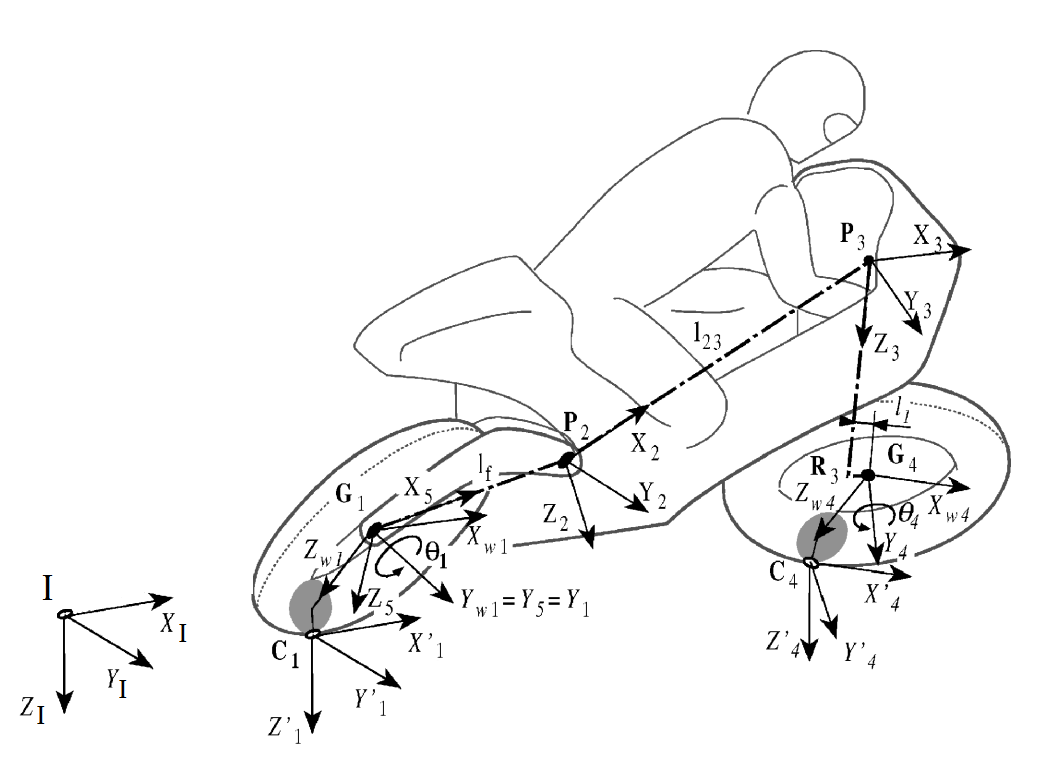
\includegraphics[width=0.85\textwidth]{abbildungen/05_Motorrad.png}
\caption{Motorrad als Mehrk\"orpersystem mit nat\"urlichen Koordinaten \cite[S. 10]{Cossalter2002}}
\label{fig:modell_motorrad}
\end{center}
\end{figure}
Das System wird mit Hilfe von zehn Koordinatensystemen beschrieben. Die Koordinatensysteme werden im Folgenden mit Hilfe ihrer zugeh\"origen homogenen Transformationsmatrizen identifiziert. Die Transformationsmatrizen $\matr{T}_{i}, i=1,\dots,10$ beinhalten jeweils eine Rotationsmatrix $\matr{R}_{i}$ und einen Ortsvektor $\vect{q}_{i}$ entsprechend \eqnref{gl:kos_transfHomog_homKoord_transfoKompl}, mit Hilfe derer ein \"Ubergang zum Inertialsystem $\KOS{I}$ m\"oglich ist. Die Komponenten von $\matr{R}_{i}$ und $\vect{q}_{i}$ sind die generalisierten Koordinaten des Systems. F\"ur zehn Koordinatensysteme werden daher, wie in Abschnitt \ref{sec:kos_natKoord} dargelegt wurde, \begin{align*}
12\cdot 10 &= 120
\end{align*} generalisierte Koordinaten eingef\"uhrt. Werden die Koordinatensysteme entsprechend dem Ansatz der nat\"urlichen Koordinaten geschickt zueinander ausgerichtet, so sinkt die Anzahl der ben\"otigten Einheitsvektoren drastisch und die Anzahl an ben\"otigten generalisierten Koordinaten wird stark reduziert. Die Systembeschreibung wird dadurch einfacher und der Rechenaufwand geringer. Auf einige dieser \"Uberlegungen wird im Folgenden Eingegangen. Die Bezeichnung einzelner Elemente weicht dabei von der Darstellung in \cite{Cossalter2002} ab, weil diese so einfacherer der Darstellung in \figureref{fig:modell_motorrad} zuzuordnen sind.  \hfill \newline
Das Inertialsystem wird durch die Einheitsvektoren \begin{align*}
\vect{c}_{x,I}&=\transp{\left(1,0,0 \right)} 
&\vect{c}_{y,I}&=\transp{\left(0,1,0 \right)}
&\vect{c}_{z,I}&=\transp{\left(0,0,1 \right)}
\end{align*} aufgespannt und durch den Ortsvektor ${\vect{O}=\transp{\left(0,0,0 \right)}}$ im Raum fixiert. Die Vektoren $\vect{c}_{x,I}$ und $\vect{c}_{y,I}$ bilden die Ebene, auf welcher sich das Motorrad bewegen kann. Die Einheitsvektoren der Koordinatensysteme werden so festgelegt, dass $\vect{u}_{i}$ in x-Richtung, $\vect{w}_{i}$ in y-Richtung und $\vect{v}_{i}$ in z-Richtung bez\"uglich $\KOS{I}$ positive Werte annehmen. \hfill \newline
Das Hinterrad wird durch drei Koordinatensysteme beschrieben. Zwei der Koordinatensysteme haben ihren Ursprung im Radmittelpunkt, das Dritte bewegt sich mit dem Kontaktpunkt zwischen Hinterreifen und Stra\ss{}e mit und wird durch $\matr{T}'_{1}$ identifiziert. Da dieser Kontaktpunkt in der Ebene, welche von $\vect{c}_{x,I}$ und $\vect{c}_{y,I}$ aufgespannt wird, liegen muss, ist die z-Komponente von $\vect{w}'_{1}$ konstant null. Der Vektor $\vect{v}'_{1}$ liegt des weiteren parallel zu $\vect{c}_{z,I}$ und ben\"otigt daher gar keine generalisierten Koordinaten.  Das Koordinatensystem $\matr{T}_{w1}$ ist so ausgerichtet, dass die x-Achse immer in Fahrtrichtung zeigt. Der Einheitsvektor $\vect{u}_{w1}$ liegt parallel zur Fahrbahn und ben\"otigt daher keine variable z-Komponente. Die x-Achsen von $\matr{T}'_{1}$ und $\matr{T}_{w1}$ werden au\ss{}erdem als parallel definiert, wodurch drei weitere generalisierte Koordinaten obsolet werden. Da alle Koordinatensysteme normierte Rechtssysteme sein sollen, stehen die Vektoren $\vect{u}'_{1}, \vect{w}'_{1}$ senkrecht aufeinander. Das System $\matr{T}'_{1}$ liegt weiterhin in einer konstanten Ebene, wodurch f\"ur die Definition von $\vect{u}'_{1}, \vect{w}'_{1}$ bereits zwei generalisierte Koordinaten ausreichen. $\matr{T}_{1}$ ist fest mit dem Hinterrad verankert und geht aus $\matr{T}_{w1}$ direkt durch Drehung um die $Y_{w1}$ Achse hervor. Diese Drehung ben\"otigt nur eine generalisierte Koordinate. Da beide Systeme den gleichen Ursprung haben, entfallen weitere drei generalisierte Koordinaten. Insgesamt stellt man fest, dass sich diese drei Koordinatensysteme durch deren geschickte Definition mit Hilfe von 15 anstelle von $12\cdot 3 = 36$ generalisierten Koordinaten $\vect{q}$ beschreiben lassen. \begin{align*}
\intertext{F\"ur $\matr{T}_{w1}$ gilt}
\vect{u}_{w1}&=\transp{\left(u_{w1,x}, u_{w1,y},0,0 \right)} 
\\
\vect{w}_{w1}&=\transp{\left(w_{w1,x}, w_{w1,y}, w_{w1,z}, 0\right)}
\\
\vect{v}_{w1}&=\transp{\left(v_{w1,x}, v_{w1,y}, v_{w1,z}, 0\right)}
\\
\vect{q}_{w1}&=\transp{\left(q_{w1,x}, q_{w1,y}, q_{w1,z}, 1\right)}.
\intertext{F\"ur $\matr{T}'_{1}$ gilt}
\vect{u}'_{1}&=\vect{u}_{w1}
\\
\vect{w}'_{1}&=\transp{\left(-u_{w1,y}, u_{w1,x}, 0, 0\right)}
\\
\vect{v}'_{1}&=\transp{\left(0, 0, 1, 0\right)}
\\
\vect{q}'_{1}&=\transp{\left(q'_{1,x}, q'_{1,y}, q'_{1,z}, 1\right)}.
\intertext{F\"ur $\matr{T}_{1}$ gilt}
\matr{T}_{1}&= \inv{\matr{T}_{rot,w1}}\matr{T}_{w1} ,
\intertext{wobei die Rotation um die Achse $Y_{w1}$ mit}
\matr{T}_{rot,w1}&=\begin{pmatrix}
\cos \left( \theta_{1}
 \right) &0&\sin \left( \theta_{1}  \right) &0\\
0&1&0&0\\ -\sin \left( \theta_{
1}   \right) &0&\cos \left( \theta_{1}  \right) &0\\ 
 0&0&0&1\end{pmatrix} 
\intertext{erfolgt.}
\intertext{F\"ur den Vektor der generalisierten Koordinaten ergibt sich damit}
\vect{q}= &\left(u_{w1,x}, u_{w1,y},w_{w1,x}, w_{w1,y}, w_{w1,z}, v_{w1,x}, v_{w1,y}, v_{w1,z},\right. \\
 & \left. q_{w1,x}, q_{w1,y}, q_{w1,z}, q'_{1,x}, q'_{1,y}, q'_{1,z}, \theta_{1}  \right)^{T}
\end{align*}
Diese \"Uberlegungen gelten f\"ur das Vorderrad analog, wobei sich das Rad nat\"urlich mit der Lenkachse mit dreht. Die Richtungsvektoren $\vect{w}_{3}$ und $\vect{w}_{w4}$ sind daher gleich.\hfill \newline
Die \"ubrigen vier Koordinatensysteme beschreiben die Lage der Hinterradschwinge, die Lenkerposition und die Lage der unged\"ampften Vorderradmassen. Die Hinterradschwinge wird mit Hilfe von $\matr{T}_{5}$ und $\matr{T}_{2}$ beschrieben. $\matr{T}_{5}$ hat seinen Ursprung an der gleichen Stelle wie $\matr{T}_{w1}$. Die x-Achse zeigt jedoch nicht gerade nach vorn, sondern auf das Gelenk, in welchem die Hinterradschwinge mit dem Motorradrahmen verbunden ist. Die Y-Achse von $\matr{T}_{5}$ ist identisch mit der von $\matr{T}_{w1}$. F\"ur die Beschreibung von $\matr{T}_{5}$ werden daher sechs neue generalisierte Koordinaten notwendig. $\matr{T}_{2}$ hat den Ursprung in der Rahmenaufh\"angung der Hinterradschwinge und eine y-Achse, welche zu der von $\matr{T}_{w1}$ parallel ist. Die Richtungsvektoren dieser Achsen sind demnach identisch. Die x-Achse von $\matr{T}_{2}$ ist so ausgerichtet, dass sie senkrecht auf der Lenkachse steht. Die zur Beschreibung dieser zwei Systeme notwendigen Vektoren lauten also \begin{align*}
\vect{u}_{2}&=\transp{\left(u_{2,x}, u_{2,y},u_{2,z},0 \right)} 
\\
\vect{w}_{2}&=\vect{w}_{w1}
\\
\vect{v}_{2}&=\transp{\left(v_{2,x}, v_{2,y}, v_{2,z}, 0\right)}
\\
\vect{q}_{2}&=\transp{\left(q_{2,x}, q_{2,y}, q_{2,z}, 1\right)}
\intertext{f\"ur $\matr{T}_{2}$ und}
\vect{u}_{5}&=\transp{\left(u_{5,x}, u_{5,y}, u_{5,z}, 0\right)}
\\
\vect{w}_{5}&=\vect{w}_{w1}
\\
\vect{v}_{5}&=\transp{\left(v_{5,x}, v_{5,y}, v_{5,z}, 0\right)}
\\
\vect{q}_{5}&=\vect{q}_{w1}
\intertext{f\"ur $\matr{T}_{5}$.}
\end{align*} Das System $\matr{T}_{3}$ wird so ausgerichtet, dass die z-Achse entlang der Lenkachse verl\"auft. Der Ursprung liegt im Schnittpunkt der Lenkachse mit der auf der Lenkachse senkrecht stehenden Ebene, welche den Ursprung von $\matr{T}_{2}$ als Element hat. Die Elemente von $\matr{T}_{3}$ lauten damit \begin{align*}
\vect{u}_{3}&=\transp{\left(u_{3,x}, u_{3,y}, u_{3,z}, 0\right)}
\\
\vect{w}_{3}&=\transp{\left(w_{3,x}, w_{3,y}, w_{3,z}, 0\right)}
\\
\vect{v}_{3}&=\vect{v}_{2}
\\
\vect{q}_{3}&=\transp{\left(q_{3,x}, q_{3,y}, q_{3,z}, 1\right)}.
\end{align*} 
Das letzte Koordinatensystem umfasst die unged\"ampften Massen am Vorderrad. Es ben\"otigt keine neuen generalisierten Koordinaten, da es sich mit Ausnahme der Rotation mit dem Vorderrad mitbewegt. \hfill \newline
Insgesamt ergeben sich durch die so definierten Koordinatensysteme also $51$ generalisierte Koordinaten, welche sich aus $15$ generalisierten Koordinaten f\"ur das Hinterrad, $15$ f\"ur die Schwinge, $9$ f\"ur den Lenker und $12$ f\"ur das Vorderrad zusammen setzen. Die vorl\"aufig berechnete Anzahl von 120 Koordinaten konnte demnach durch geeignete Festlegung der Koordinatensysteme zueinander um mehr als die H\"alfte reduziert werden. \hfill \newline

Die Anzahl generalisierter Koordinaten ist immer noch hoch. In Folge der Modellierung mit nat\"urlichen Koordinaten lassen sich aber im n\"achsten Schritt die Zwangsbedingungen auf sehr einfache Art formulieren. Wie im Abschnitt \ref{sec:kos_natKoord} dargelegt wurde, m\"ussen alle Vektoren $\vect{u}_{i}, \vect{w}_{i}, \vect{v}_{i}$ Einheitsl\"ange haben und senkrecht aufeinander stehen. Diese Bedingungen lassen sich auf triviale Weise mit dem Skalarprodukt formulieren. Stellt man diese Bedingungen f\"ur alle eingef\"uhrten Richtungsvektoren auf, so ergeben sich 26 Zwangsbedingungen. Mit Hilfe weiterer Gleichungen kann die Geometrie des Motorrads beschrieben werden.\hfill \newline
Beispielhaft sei die konstante L\"ange der Hinterradschwinge betrachtet. Durch die geschickte Wahl der Koordinatenurspr\"unge von $\matr{T}_{w1}$ und $\matr{T}_{2}$ ist die Gleichung sehr einfach aufzustellen. Sei die Schwingenl\"ange durch den Parameter $l_{schw}$ gegeben. Die geforderte konstante L\"ange l\"asst sich dann mit dem Skalarprodukt als \begin{align*}
\skalar{\vect{q}_{2}-\vect{q}_{w1}}{\vect{q}_{2}-\vect{q}_{w1}} - l_{schw}^{2}&=0
\end{align*} formulieren. Dabei ist darauf zu achten, dass die Zwangsbedingung der Form $\phi\of{\vect{q}}=0$ entspricht. Auf \"ahnliche Weise lassen sich sieben weitere geometrische Beziehungen als Zwangsbedingungen formulieren. Dabei sind alle Gleichungen frei von trigonometrischen Funktionen. In Folge dessen l\"asst sich die Jacobimatrix der Zwangsbedingungen $\Phi_{\vect{q}}\of{\vect{q}}$ einfach berechnen. \hfill \newline
Die generalisierten Koordinaten k\"onnten mit Hilfe der Zwangsbedingungen auf einen Satz Minimalkoordinaten reduziert werden. Dieser Ansatz ist aber nicht zweckm\"a\ss{}ig, da der Rechenaufwand f\"ur die algebraische Umformung sehr hoch ist und die erhaltenen Ausdr\"ucke f\"ur die Minimalkoordinaten sehr komplex w\"aren. Daher verwendet man zur L\"osung des Systems den Ansatz von Langrange \mbox{2. Art}, wie er in \eqnref{gl:mech_lagrange2ArtDefCossalter} angegeben ist. \hfill \newline

Der zur L\"osung von \eqnref{gl:mech_lagrange2ArtDefCossalter} ben\"otigte Ausdruck f\"ur die kinetische Energie wurde bereits in Abschnitt \ref{ssec:mech_lag2_kinEn} ausf\"uhrlich hergeleitet. Mit Hilfe der generalisierten Koordinaten, den Schwerpunktkoordinaten und den Elementen des Tr\"agheitstensors kann die Gleichung f\"ur die kinetische Energie nach \eqnref{gl:mech_lag2_kinEn_kinEnHomogAllg} direkt aufgestellt werden. Dabei ist lediglich darauf zu achten, dass nur die Systeme $\matr{T}_{w1}, \matr{T}_{2}, \matr{T}_{3}, \matr{T}_{w4}, \matr{T}_{5}$ und $\matr{T}_{6}$ in diese Gleichung eingehen. Die \"ubrigen vier Koordinatensysteme werden ausschlie\ss{}lich zur Beschreibung der Reifenbewegung und der Reifenkr\"afte ben\"otigt. \hfill \newline

Die Formulierung der virtuellen Arbeit und die Umformung zu generalisierten Kr\"aften ist keine triviale Aufgabe. Als Beispiel der Anwendung der in Abschnitt \ref{ssec:mech_lag2_virtArbeit} hergeleiteten Gleichungen sollen die virtuelle Arbeit der Gravitation und der am Hinterrad wirkenden Reifenkr\"afte erl\"autert werden.  \cite[S.14 f.]{Cossalter2002}\hfill \newline
Die Gravitationskraft l\"asst sich mit Hilfe der Erdbeschleunigung $g$ und der Masse eines K\"orpers bestimmen. Notiert man die Erdbeschleunigung unter Beachtung ihrer Wirkrichtung als homogenen Vektor mit $\vect{g}=\transp{\left(0,0,g,1 \right)}$ und multipliziert diesen mit der K\"orpermasse und der virtuellen Verschiebung des K\"orperschwerpunkts, so erh\"alt man die virtuelle Arbeit der Gravitationskraft. Es ergibt sich f\"ur einen K\"orper $i$ \begin{align*}
\delta W_{g,i}&= m_{i} \skalar{\vect{g}}{\delta\of{\tensor*[^K_I]{\matr{T}}{_i}\vect{\tensor*[_K]{S}{_i}}}},
\end{align*} wobei mit $\vect{\tensor*[_K]{S}{_i}}$ der konstante Schwerpunkt des K\"orpers in Relation zu seinem k\"orperfesten Koordinatensystem gegeben ist. Wendet man den Operator der virtuellen Verschiebung auf alle Elemente von $\tensor*[^K_I]{\matr{T}}{}$ entsprechend \eqnref{gl:mathGrundl_vektorraeume_matr_diff} an und beachtet die Umformungsregeln aus \eqnref{gl:mech_lag2_virtArbeit_genVersch}, so folgt \begin{align*}
\delta\of{\tensor*[^K_I]{\matr{T}}{_i}\vect{\tensor*[_K]{S}{_i}}}&= \delta 
\begin{pmatrix}
  \tensor*[_I]{u}{_{i,x}}& \tensor*[_I]{w}{_{i,x}}& \tensor*[_I]{v}{_{i,x}} & \tensor*[_I]{q}{_{i,x}} \\ 
  \tensor*[_I]{u}{_{i,y}}& \tensor*[_I]{w}{_{i,y}}& \tensor*[_I]{v}{_{i,y}} & \tensor*[_I]{q}{_{i,y}} \\ 
  \tensor*[_I]{u}{_{i,z}}& \tensor*[_I]{w}{_{i,z}}& \tensor*[_I]{v}{_{i,z}} & \tensor*[_I]{q}{_{i,z}} \\
  0 & 0 & 0 & 1
  \end{pmatrix} \begin{bmatrix}
  \tensor*[_K]{S}{_{i,x}} \\
  \tensor*[_K]{S}{_{i,y}} \\
  \tensor*[_K]{S}{_{i,z}} \\
  1
  \end{bmatrix} \\
  &= \delta \begin{bmatrix}  \tensor*[_I]{u}{_{i,x}}\, \tensor*[_K]{S}{_{i,x}}+ \tensor*[_I]{w}{_{i,x}}\, \tensor*[_K]{S}{_{i,y}}+ \tensor*[_I]{v}{_{i,x}}\, \tensor*[_K]{S}{_{i,z}}+q_{i,x} \\ 
 \tensor*[_I]{u}{_{i,y}}\, \tensor*[_K]{S}{_{i,x}}+ \tensor*[_I]{w}{_{i,y}}\, \tensor*[_K]{S}{_{i,y}}+ \tensor*[_I]{v}{_{i,y}}\, \tensor*[_K]{S}{_{i,z}}+q_{i,y}\\ 
 \tensor*[_I]{u}{_{i,z}}\, \tensor*[_K]{S}{_{i,x}}+ \tensor*[_I]{w}{_{i,z}}\, \tensor*[_K]{S}{_{i,y}}+ \tensor*[_I]{v}{_{i,z}}\, \tensor*[_K]{S}{_{i,z}}+q_{i,z}\\
1 \end{bmatrix} \\
&= \frac{\d}{\d \vect{q}} \begin{bmatrix}  \tensor*[_I]{u}{_{i,x}}\, \tensor*[_K]{S}{_{i,x}}+ \tensor*[_I]{w}{_{i,x}}\, \tensor*[_K]{S}{_{i,y}}+ \tensor*[_I]{v}{_{i,x}}\, \tensor*[_K]{S}{_{i,z}}+q_{i,x} \\ 
 \tensor*[_I]{u}{_{i,y}}\, \tensor*[_K]{S}{_{i,x}}+ \tensor*[_I]{w}{_{i,y}}\, \tensor*[_K]{S}{_{i,y}}+ \tensor*[_I]{v}{_{i,y}}\, \tensor*[_K]{S}{_{i,z}}+q_{i,y}\\ 
 \tensor*[_I]{u}{_{i,z}}\, \tensor*[_K]{S}{_{i,x}}+ \tensor*[_I]{w}{_{i,z}}\, \tensor*[_K]{S}{_{i,y}}+ \tensor*[_I]{v}{_{i,z}}\, \tensor*[_K]{S}{_{i,z}}+q_{i,z}\\
1 \end{bmatrix} \delta \vect{q}
\end{align*} 
f\"ur die virtuelle Verschiebung des Schwerpunkts. Die virtuelle Arbeit ergibt sich damit durch geeignete Umformung zu \begin{align*}
\delta W_{g,i}&= m_{i} \skalar{\vect{g}}{\delta\of{\tensor*[^K_I]{\matr{T}}{_i}\vect{\tensor*[_K]{S}{_i}}}} \\
&= m_{i} \skalar{\delta\of{\tensor*[^K_I]{\matr{T}}{_i}\vect{\tensor*[_K]{S}{_i}}}}{\vect{g}} 
\\
&= m_{i} \transp{\left( \delta\of{\tensor*[^K_I]{\matr{T}}{_i}\vect{\tensor*[_K]{S}{_i}}} \right) }\vect{g}.
\end{align*} In ausf\"uhrlicher Notation f\"uhrt dies auf
\begin{align*}
\delta W_{g,i}&= m_{i} \left( \frac{\d}{\d \vect{q}} \begin{bmatrix}  \tensor*[_I]{u}{_{i,x}}\, \tensor*[_K]{S}{_{i,x}}+ \tensor*[_I]{w}{_{i,x}}\, \tensor*[_K]{S}{_{i,y}}+ \tensor*[_I]{v}{_{i,x}}\, \tensor*[_K]{S}{_{i,z}}+q_{i,x} \\ 
 \tensor*[_I]{u}{_{i,y}}\, \tensor*[_K]{S}{_{i,x}}+ \tensor*[_I]{w}{_{i,y}}\, \tensor*[_K]{S}{_{i,y}}+ \tensor*[_I]{v}{_{i,y}}\, \tensor*[_K]{S}{_{i,z}}+q_{i,y}\\ 
 \tensor*[_I]{u}{_{i,z}}\, \tensor*[_K]{S}{_{i,x}}+ \tensor*[_I]{w}{_{i,z}}\, \tensor*[_K]{S}{_{i,y}}+ \tensor*[_I]{v}{_{i,z}}\, \tensor*[_K]{S}{_{i,z}}+q_{i,z}\\
1 \end{bmatrix} \delta \vect{q} \right)^{T} \vect{g} 
\\
&= \transp{\delta \vect{q}} \com{m_{i} \left( \frac{\d}{\d \vect{q}} \begin{bmatrix}  \tensor*[_I]{u}{_{i,x}}\, \tensor*[_K]{S}{_{i,x}}+ \tensor*[_I]{w}{_{i,x}}\, \tensor*[_K]{S}{_{i,y}}+ \tensor*[_I]{v}{_{i,x}}\, \tensor*[_K]{S}{_{i,z}}+q_{i,x} \\ 
 \tensor*[_I]{u}{_{i,y}}\, \tensor*[_K]{S}{_{i,x}}+ \tensor*[_I]{w}{_{i,y}}\, \tensor*[_K]{S}{_{i,y}}+ \tensor*[_I]{v}{_{i,y}}\, \tensor*[_K]{S}{_{i,z}}+q_{i,y}\\ 
 \tensor*[_I]{u}{_{i,z}}\, \tensor*[_K]{S}{_{i,x}}+ \tensor*[_I]{w}{_{i,z}}\, \tensor*[_K]{S}{_{i,y}}+ \tensor*[_I]{v}{_{i,z}}\, \tensor*[_K]{S}{_{i,z}}+q_{i,z}\\
1 \end{bmatrix} \right)^{T} \begin{bmatrix}
0 \\ 0 \\ g \\ 1
\end{bmatrix}}{$\matr{Q}_{g,i}$}
\end{align*} und man erh\"alt einen Ausdruck f\"ur die generalisierte Kraft, welche durch die Gravitation entsteht. Der Term $\matr{Q}_{g,i}$ hat die in \eqnref{gl:mech_lag2_virtArbeit_genKraft} und \eqnref{gl:virtWgenF} geforderte Form und ist daher zur L\"osung von \eqnref{gl:mech_lagrange2ArtDefCossalter} geeignet. 

\begin{figure}[h!tb]
\begin{center}
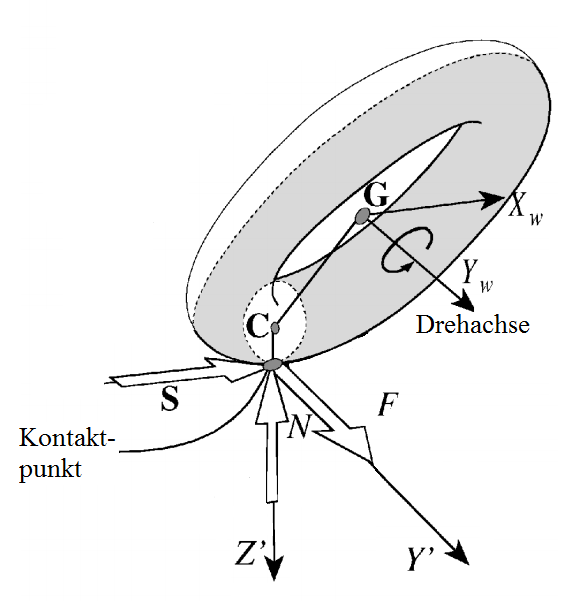
\includegraphics[width=0.5\textwidth]{abbildungen/05_reifenkraefte.png}
\caption{Reifenkr\"afte im Kontaktpunkt von Stra\ss{}e und Reifen \cite[S. 6]{Cossalter2002}}
\label{fig:modell_reifenF}
\end{center}
\end{figure}

Der Kraftvektor der Reifenkr\"afte soll im Kontaktpunkt zwischen Hinterrad und Stra\ss{}e angreifen, wie es in \figureref{fig:modell_reifenF} abgebildet wird. Die definierten Kr\"afte  sind dann mit Hilfe von $\matr{T}'_{1}$ in das Inertialsystem transformierbar und es gilt \begin{align*}
\vect{\tensor*[_I]{F}{_{T1}}}&=\matr{T}_{1}' \vect{\tensor*[_K]{F}{_{T1}}}.
\end{align*} Sind die Reifenkr\"afte im Inertialsystem bekannt, so muss deren Einfluss auf die virtuelle Arbeit durch eine virtuelle Verschiebung und eine virtuelle Rotation modelliert werden. F\"ur den ersten Term ist die Verschiebung des Reifenmittelpunktes $\vect{\tensor*[_I]{S}{_{w1}}}$ von Interesse. Es gilt \begin{align*}
\delta W_{T1,S}&= \vect{\tensor*[_I]{F}{_{T1}}} \delta \vect{\tensor*[_I]{S}{_{w1}}}.
\end{align*} Da der Reifenmittelpunkt gleich dem Ursprung von $\matr{T}_{w1}$ ist, vereinfacht sich diese Gleichung zu \begin{align*}
\delta W_{T1,S}&= \vect{\tensor*[_I]{F}{_{T1}}} \delta \vect{q}_{w1}.
\end{align*} F\"ur den Term der virtuellen Arbeit, welcher durch virtuelle Rotation entsteht, wird der Vektor $\vect{a}_{T1}$ ben\"otigt, welcher den Schwerpunkt des Hinterrades mit dem Kraftangriffspunkt der Reifenkr\"afte verbindet. Da dieser Vektor offensichtlich die Urspr\"unge der Systeme $\matr{T}_{w1}$ und $\matr{T}_{1}'$ verbindet, lautet er\begin{align*}
\vect{a}_{T1}&=\vect{q}'_{1} - \vect{q}_{w1}.
\end{align*} Die virtuelle Arbeit lautet dann \begin{align*}
\delta W_{T1,rot}&= \skalar{\vect{a}_{T1} \times \vect{\tensor*[_I]{F}{_{T1}}}}{\matr{T}_{1} \delta \vect{\tensor*[_{T1}]{\phi}{}}\of{\matr{T}_{1}}},
\end{align*} wobei der Term $\delta \vect{\tensor*[_{T1}]{\phi}{}}\of{\matr{T}_{1}}$ der lokalen virtuellen Rotation von $\matr{T}_{1}$ entspricht, wie er allgemein in \eqnref{gl:mech_lag2_virtArbeit_virtRotMatr} hergeleitet wurde. Die gesamte virtuelle Arbeit der Reifenkr\"afte des Hinterrades lautet damit \begin{align*}
\delta W_{W1} = \delta W_{T1,S} + \delta W_{T1,rot} &= \vect{\tensor*[_I]{F}{_{T1}}} \delta \vect{q}_{w1} \skalar{\vect{a}_{T1} \times \vect{\tensor*[_I]{F}{_{T1}}}}{\matr{T}_{1} \delta \vect{\tensor*[_{T1}]{\phi}{}}\of{\matr{T}_{1}}}
\end{align*} Mit den bereits angewandten Umformungsschritten l\"asst sich auch diese Gleichung in eine generalisierte Arbeit und die virtuelle Verschiebung der generalisierten Koordinaten zerlegen. \hfill \newline
Die weiteren Gleichungen, welche notwendig sind, um die gesamte virtuelle Arbeit zu berechnen, sind in \cite[S.14 f.]{Cossalter2002} angegeben. \hfill \newline

Die genaue Modellierung der Reifen ist ein besonderes Merkmal der Arbeit \cite{Cossalter2002}. Es wird das Reifenmodell, welches in \cite{Lot2004} ver\"offentlicht wurde, verwendet. Es zeichnet sich dadurch aus, dass der genaue Kontaktpunkt zwischen Reifen und Stra\ss{}e betrachtet wird. Dies wird m\"oglich, indem der Reifen als verformbar angenommen wird. In Folge dieser Modellierung sind die Kennwerte, welche zur Charakterisierung des Reifenverhaltens notwendig sind, von geringer Anzahl und mit vergleichsweise wenig Aufwand messtechnisch zu erfassen.   
%\chapter{Implementierung}\label{ch:implement}

\section{Notwendige Suchbefehle zum Ersetzen der Differentiation}
Suche nach: \begin{lstlisting}
diff\(diff\(([a-z]+__\d+\(t\),) t\), t\)
\end{lstlisting} 

ersetzen durch: 
\begin{lstlisting} 
diff\($1 t, 2\)
\end{lstlisting} 

Ergebnis entspricht der Matlab Vorgabe fuer mehrfache Ableitung: 
\begin{lstlisting}
diff(expr, var, int)
\end{lstlisting}

Maple verwendet f\"ur die Signum-Funktion den Betrag in der Form
\begin{lstlisting}
\abs(1,expr)
\end{lstlisting}
In Matlab muss dieser Ausdruck also wie folgt ersetzt werden:
\begin{lstlisting}
\sign(expr)
\end{lstlisting}

\section{Stabilisierung nach Baumgarte}
Untersuchungen zu der Wahl der Parameter finden sich unter anderem in:
, \cite{Flores2011}-> gute D\"ampfung f\"ur gleiche Parameter,\cite{Neto2003}$\alpha, \beta$ h\"aufig gleich 5 gew\"ahlt.

\section{\"Ubersichtswerke zur L\"osung von DAEs}
\cite{Haug1991}, \cite{ErnstHairer2010}

\section{Alternative Stabilisierungsverfahren}
\cite{Park1988},\cite{Cline2003}

\section{Fortran}
Notwendige Schritte:
\begin{enumerate}
\item fortran-compiler installieren (z. B. gfortran, welcher in cygwin64 enthalten ist)
\item die Path-Variable von Windoof updaten
\item Windows-Konsole \"offnen
\item im Make-File sicherstellen, dass der compiler \glqq gfortran\grqq ausgew\"ahlt ist
\item Make-File starten: \$make -f <makefileName>
\end{enumerate}
%
% Anhang (Bibliographie darf im deutschen nicht in den Anhang!)
%\bibliography{bib/quellen}

\nocite{*}%alle Elemente im Literaturverzeichnis werden aufgelistet, auch die nicht-zitierten
\printbibliography[title={Literaturverzeichnis}]
\pagenumbering{Roman} %neue Seitenzahlen
\stepcounter{chapter}
\addcontentsline{toc}{chapter}{\protect\numberline{\thechapter}{Literaturverzeichnis}}
\cleardoublepage
%
%% Anhang
%\backmatter
%\appendix
%\chapter{Anhang mit Sachen}
\label{cha:anhang_uebungen}

%
%\IfDefined{printindex}{\printindex}
%\IfDefined{printnomenclature}{\printnomenclature}
%\cleardoublepage
%\leerseite{}
%\cleardoublepage


\end{document}

